\documentclass[twoside]{book}

% Packages required by doxygen
\usepackage{fixltx2e}
\usepackage{calc}
\usepackage{doxygen}
\usepackage[export]{adjustbox} % also loads graphicx
\usepackage{graphicx}
\usepackage[utf8]{inputenc}
\usepackage{makeidx}
\usepackage{multicol}
\usepackage{multirow}
\PassOptionsToPackage{warn}{textcomp}
\usepackage{textcomp}
\usepackage[nointegrals]{wasysym}
\usepackage[table]{xcolor}

% Font selection
\usepackage[T1]{fontenc}
\usepackage[scaled=.90]{helvet}
\usepackage{courier}
\usepackage{amssymb}
\usepackage{sectsty}
\renewcommand{\familydefault}{\sfdefault}
\allsectionsfont{%
  \fontseries{bc}\selectfont%
  \color{darkgray}%
}
\renewcommand{\DoxyLabelFont}{%
  \fontseries{bc}\selectfont%
  \color{darkgray}%
}
\newcommand{\+}{\discretionary{\mbox{\scriptsize$\hookleftarrow$}}{}{}}

% Page & text layout
\usepackage{geometry}
\geometry{%
  a4paper,%
  top=2.5cm,%
  bottom=2.5cm,%
  left=2.5cm,%
  right=2.5cm%
}
\tolerance=750
\hfuzz=15pt
\hbadness=750
\setlength{\emergencystretch}{15pt}
\setlength{\parindent}{0cm}
\setlength{\parskip}{3ex plus 2ex minus 2ex}
\makeatletter
\renewcommand{\paragraph}{%
  \@startsection{paragraph}{4}{0ex}{-1.0ex}{1.0ex}{%
    \normalfont\normalsize\bfseries\SS@parafont%
  }%
}
\renewcommand{\subparagraph}{%
  \@startsection{subparagraph}{5}{0ex}{-1.0ex}{1.0ex}{%
    \normalfont\normalsize\bfseries\SS@subparafont%
  }%
}
\makeatother

% Headers & footers
\usepackage{fancyhdr}
\pagestyle{fancyplain}
\fancyhead[LE]{\fancyplain{}{\bfseries\thepage}}
\fancyhead[CE]{\fancyplain{}{}}
\fancyhead[RE]{\fancyplain{}{\bfseries\leftmark}}
\fancyhead[LO]{\fancyplain{}{\bfseries\rightmark}}
\fancyhead[CO]{\fancyplain{}{}}
\fancyhead[RO]{\fancyplain{}{\bfseries\thepage}}
\fancyfoot[LE]{\fancyplain{}{}}
\fancyfoot[CE]{\fancyplain{}{}}
\fancyfoot[RE]{\fancyplain{}{\bfseries\scriptsize Generated by Doxygen }}
\fancyfoot[LO]{\fancyplain{}{\bfseries\scriptsize Generated by Doxygen }}
\fancyfoot[CO]{\fancyplain{}{}}
\fancyfoot[RO]{\fancyplain{}{}}
\renewcommand{\footrulewidth}{0.4pt}
\renewcommand{\chaptermark}[1]{%
  \markboth{#1}{}%
}
\renewcommand{\sectionmark}[1]{%
  \markright{\thesection\ #1}%
}

% Indices & bibliography
\usepackage{natbib}
\usepackage[titles]{tocloft}
\setcounter{tocdepth}{3}
\setcounter{secnumdepth}{5}
\makeindex

% Hyperlinks (required, but should be loaded last)
\usepackage{ifpdf}
\ifpdf
  \usepackage[pdftex,pagebackref=true]{hyperref}
\else
  \usepackage[ps2pdf,pagebackref=true]{hyperref}
\fi
\hypersetup{%
  colorlinks=true,%
  linkcolor=blue,%
  citecolor=blue,%
  unicode%
}

% Custom commands
\newcommand{\clearemptydoublepage}{%
  \newpage{\pagestyle{empty}\cleardoublepage}%
}

\usepackage{caption}
\captionsetup{labelsep=space,justification=centering,font={bf},singlelinecheck=off,skip=4pt,position=top}

%===== C O N T E N T S =====

\begin{document}

% Titlepage & ToC
\hypersetup{pageanchor=false,
             bookmarksnumbered=true,
             pdfencoding=unicode
            }
\pagenumbering{alph}
\begin{titlepage}
\vspace*{7cm}
\begin{center}%
{\Large Drum\+Pi }\\
\vspace*{1cm}
{\large Generated by Doxygen 1.8.13}\\
\end{center}
\end{titlepage}
\clearemptydoublepage
\pagenumbering{roman}
\tableofcontents
\clearemptydoublepage
\pagenumbering{arabic}
\hypersetup{pageanchor=true}

%--- Begin generated contents ---
\chapter{Drum\+Pi}
\label{index}\hypertarget{index}{}A drum machine made for the Raspberry Pi. \begin{DoxyVersion}{Version}
1.\+0 
\end{DoxyVersion}
\begin{DoxyAuthor}{Authors}
Stuart Ball \href{mailto:2260112B@student.gla.ac.uk}{\tt 2260112\+B@student.\+gla.\+ac.\+uk} 

Murdo Graham \href{mailto:2261517G@student.gla.ac.uk}{\tt 2261517\+G@student.\+gla.\+ac.\+uk} 

Finn Quicke \href{mailto:2256694Q@student.gla.ac.uk}{\tt 2256694\+Q@student.\+gla.\+ac.\+uk} 
\end{DoxyAuthor}
\begin{DoxyDate}{Date}
April 2021 
\end{DoxyDate}

\chapter{Namespace Index}
\doxysection{Namespace List}
Here is a list of all documented namespaces with brief descriptions\+:\begin{DoxyCompactList}
\item\contentsline{section}{\mbox{\hyperlink{namespacedrumpi}{drumpi}} }{\pageref{namespacedrumpi}}{}
\item\contentsline{section}{\mbox{\hyperlink{namespacedrumpi_1_1audio}{drumpi\+::audio}} }{\pageref{namespacedrumpi_1_1audio}}{}
\item\contentsline{section}{\mbox{\hyperlink{namespacedrumpi_1_1clock}{drumpi\+::clock}} }{\pageref{namespacedrumpi_1_1clock}}{}
\end{DoxyCompactList}

\chapter{Hierarchical Index}
\doxysection{Class Hierarchy}
This inheritance list is sorted roughly, but not completely, alphabetically\+:\begin{DoxyCompactList}
\item \contentsline{section}{drumpi\+::\+\_\+\+Sequence\+Step}{\pageref{classdrumpi_1_1__SequenceStep}}{}
\item \contentsline{section}{drumpi\+::Application\+Callback}{\pageref{classdrumpi_1_1ApplicationCallback}}{}
\begin{DoxyCompactList}
\item \contentsline{section}{drumpi\+::Application}{\pageref{classdrumpi_1_1Application}}{}
\end{DoxyCompactList}
\item \contentsline{section}{drumpi\+::audio\+::Audio\+Callback}{\pageref{classdrumpi_1_1audio_1_1AudioCallback}}{}
\begin{DoxyCompactList}
\item \contentsline{section}{drumpi\+::audio\+::Playback\+Engine}{\pageref{classdrumpi_1_1audio_1_1PlaybackEngine}}{}
\end{DoxyCompactList}
\item \contentsline{section}{drumpi\+::audio\+::Audio\+Library}{\pageref{classdrumpi_1_1audio_1_1AudioLibrary}}{}
\item Cpp\+Thread\begin{DoxyCompactList}
\item \contentsline{section}{drumpi\+::Keyboard\+Thread}{\pageref{classdrumpi_1_1KeyboardThread}}{}
\end{DoxyCompactList}
\item Cpp\+Timer\begin{DoxyCompactList}
\item \contentsline{section}{drumpi\+::clock\+::Clock}{\pageref{classdrumpi_1_1clock_1_1Clock}}{}
\begin{DoxyCompactList}
\item \contentsline{section}{drumpi\+::clock\+::Metronome}{\pageref{classdrumpi_1_1clock_1_1Metronome}}{}
\begin{DoxyCompactList}
\item \contentsline{section}{drumpi\+::Sequencer\+Clock}{\pageref{classdrumpi_1_1SequencerClock}}{}
\end{DoxyCompactList}
\item \contentsline{section}{drumpi\+::Display\+Clock}{\pageref{classdrumpi_1_1DisplayClock}}{}
\end{DoxyCompactList}
\item \contentsline{section}{drumpi\+::clock\+::Timer}{\pageref{classdrumpi_1_1clock_1_1Timer}}{}
\begin{DoxyCompactList}
\item \contentsline{section}{drumpi\+::Display\+Delay}{\pageref{classdrumpi_1_1DisplayDelay}}{}
\end{DoxyCompactList}
\end{DoxyCompactList}
\item \contentsline{section}{drumpi\+::audio\+::Jack\+Client}{\pageref{classdrumpi_1_1audio_1_1JackClient}}{}
\item \contentsline{section}{drumpi\+::Keyboard\+Input}{\pageref{classdrumpi_1_1KeyboardInput}}{}
\item \contentsline{section}{drumpi\+::Max7219}{\pageref{classdrumpi_1_1Max7219}}{}
\begin{DoxyCompactList}
\item \contentsline{section}{drumpi\+::Display}{\pageref{classdrumpi_1_1Display}}{}
\end{DoxyCompactList}
\item \contentsline{section}{drumpi\+::audio\+::Sample\+Source}{\pageref{classdrumpi_1_1audio_1_1SampleSource}}{}
\begin{DoxyCompactList}
\item \contentsline{section}{drumpi\+::audio\+::Sample\+Source\+File}{\pageref{classdrumpi_1_1audio_1_1SampleSourceFile}}{}
\begin{DoxyCompactList}
\item \contentsline{section}{drumpi\+::audio\+::Audio\+Clip}{\pageref{classdrumpi_1_1audio_1_1AudioClip}}{}
\end{DoxyCompactList}
\end{DoxyCompactList}
\item \contentsline{section}{drumpi\+::Sequencer}{\pageref{classdrumpi_1_1Sequencer}}{}
\item \contentsline{section}{drumpi\+::State}{\pageref{classdrumpi_1_1State}}{}
\begin{DoxyCompactList}
\item \contentsline{section}{drumpi\+::Performance\+Mode}{\pageref{classdrumpi_1_1PerformanceMode}}{}
\item \contentsline{section}{drumpi\+::Sequencer\+Mode}{\pageref{classdrumpi_1_1SequencerMode}}{}
\item \contentsline{section}{drumpi\+::Set\+Drum\+Bank\+Mode}{\pageref{classdrumpi_1_1SetDrumBankMode}}{}
\item \contentsline{section}{drumpi\+::Set\+Drum\+Volume\+Mode}{\pageref{classdrumpi_1_1SetDrumVolumeMode}}{}
\item \contentsline{section}{drumpi\+::Set\+Master\+Volume\+Mode}{\pageref{classdrumpi_1_1SetMasterVolumeMode}}{}
\item \contentsline{section}{drumpi\+::Set\+Tempo\+Mode}{\pageref{classdrumpi_1_1SetTempoMode}}{}
\end{DoxyCompactList}
\end{DoxyCompactList}

\chapter{Class Index}
\section{Class List}
Here are the classes, structs, unions and interfaces with brief descriptions\+:\begin{DoxyCompactList}
\item\contentsline{section}{\hyperlink{classdrumpi_1_1__SequenceStep}{drumpi\+::\+\_\+\+Sequence\+Step} }{\pageref{classdrumpi_1_1__SequenceStep}}{}
\item\contentsline{section}{\hyperlink{classdrumpi_1_1Application}{drumpi\+::\+Application} \\*Main application }{\pageref{classdrumpi_1_1Application}}{}
\item\contentsline{section}{\hyperlink{classdrumpi_1_1ApplicationCallback}{drumpi\+::\+Application\+Callback} }{\pageref{classdrumpi_1_1ApplicationCallback}}{}
\item\contentsline{section}{\hyperlink{classdrumpi_1_1audio_1_1AudioCallback}{drumpi\+::audio\+::\+Audio\+Callback} }{\pageref{classdrumpi_1_1audio_1_1AudioCallback}}{}
\item\contentsline{section}{\hyperlink{classdrumpi_1_1audio_1_1AudioClip}{drumpi\+::audio\+::\+Audio\+Clip} }{\pageref{classdrumpi_1_1audio_1_1AudioClip}}{}
\item\contentsline{section}{\hyperlink{classdrumpi_1_1audio_1_1AudioLibrary}{drumpi\+::audio\+::\+Audio\+Library} }{\pageref{classdrumpi_1_1audio_1_1AudioLibrary}}{}
\item\contentsline{section}{\hyperlink{classdrumpi_1_1clock_1_1Clock}{drumpi\+::clock\+::\+Clock} }{\pageref{classdrumpi_1_1clock_1_1Clock}}{}
\item\contentsline{section}{\hyperlink{classdrumpi_1_1Display}{drumpi\+::\+Display} }{\pageref{classdrumpi_1_1Display}}{}
\item\contentsline{section}{\hyperlink{classdrumpi_1_1DisplayClock}{drumpi\+::\+Display\+Clock} }{\pageref{classdrumpi_1_1DisplayClock}}{}
\item\contentsline{section}{\hyperlink{classdrumpi_1_1DisplayDelay}{drumpi\+::\+Display\+Delay} }{\pageref{classdrumpi_1_1DisplayDelay}}{}
\item\contentsline{section}{\hyperlink{classdrumpi_1_1audio_1_1JackClient}{drumpi\+::audio\+::\+Jack\+Client} }{\pageref{classdrumpi_1_1audio_1_1JackClient}}{}
\item\contentsline{section}{\hyperlink{classdrumpi_1_1KeyboardInput}{drumpi\+::\+Keyboard\+Input} }{\pageref{classdrumpi_1_1KeyboardInput}}{}
\item\contentsline{section}{\hyperlink{classdrumpi_1_1KeyboardThread}{drumpi\+::\+Keyboard\+Thread} }{\pageref{classdrumpi_1_1KeyboardThread}}{}
\item\contentsline{section}{\hyperlink{classdrumpi_1_1Max7219}{drumpi\+::\+Max7219} }{\pageref{classdrumpi_1_1Max7219}}{}
\item\contentsline{section}{\hyperlink{classdrumpi_1_1clock_1_1Metronome}{drumpi\+::clock\+::\+Metronome} }{\pageref{classdrumpi_1_1clock_1_1Metronome}}{}
\item\contentsline{section}{\hyperlink{classdrumpi_1_1PerformanceMode}{drumpi\+::\+Performance\+Mode} }{\pageref{classdrumpi_1_1PerformanceMode}}{}
\item\contentsline{section}{\hyperlink{classdrumpi_1_1audio_1_1PlaybackEngine}{drumpi\+::audio\+::\+Playback\+Engine} }{\pageref{classdrumpi_1_1audio_1_1PlaybackEngine}}{}
\item\contentsline{section}{\hyperlink{classdrumpi_1_1audio_1_1SampleSource}{drumpi\+::audio\+::\+Sample\+Source} }{\pageref{classdrumpi_1_1audio_1_1SampleSource}}{}
\item\contentsline{section}{\hyperlink{classdrumpi_1_1audio_1_1SampleSourceFile}{drumpi\+::audio\+::\+Sample\+Source\+File} }{\pageref{classdrumpi_1_1audio_1_1SampleSourceFile}}{}
\item\contentsline{section}{\hyperlink{classdrumpi_1_1Sequencer}{drumpi\+::\+Sequencer} }{\pageref{classdrumpi_1_1Sequencer}}{}
\item\contentsline{section}{\hyperlink{classdrumpi_1_1SequencerClock}{drumpi\+::\+Sequencer\+Clock} }{\pageref{classdrumpi_1_1SequencerClock}}{}
\item\contentsline{section}{\hyperlink{classdrumpi_1_1SequencerMode}{drumpi\+::\+Sequencer\+Mode} }{\pageref{classdrumpi_1_1SequencerMode}}{}
\item\contentsline{section}{\hyperlink{classdrumpi_1_1SetDrumBankMode}{drumpi\+::\+Set\+Drum\+Bank\+Mode} }{\pageref{classdrumpi_1_1SetDrumBankMode}}{}
\item\contentsline{section}{\hyperlink{classdrumpi_1_1SetDrumVolumeMode}{drumpi\+::\+Set\+Drum\+Volume\+Mode} }{\pageref{classdrumpi_1_1SetDrumVolumeMode}}{}
\item\contentsline{section}{\hyperlink{classdrumpi_1_1SetMasterVolumeMode}{drumpi\+::\+Set\+Master\+Volume\+Mode} }{\pageref{classdrumpi_1_1SetMasterVolumeMode}}{}
\item\contentsline{section}{\hyperlink{classdrumpi_1_1SetTempoMode}{drumpi\+::\+Set\+Tempo\+Mode} }{\pageref{classdrumpi_1_1SetTempoMode}}{}
\item\contentsline{section}{\hyperlink{classdrumpi_1_1State}{drumpi\+::\+State} }{\pageref{classdrumpi_1_1State}}{}
\item\contentsline{section}{\hyperlink{classdrumpi_1_1clock_1_1Timer}{drumpi\+::clock\+::\+Timer} }{\pageref{classdrumpi_1_1clock_1_1Timer}}{}
\end{DoxyCompactList}

\chapter{Namespace Documentation}
\hypertarget{namespacedrumpi}{}\doxysection{drumpi Namespace Reference}
\label{namespacedrumpi}\index{drumpi@{drumpi}}
\doxysubsection*{Namespaces}
\begin{DoxyCompactItemize}
\item 
 \mbox{\hyperlink{namespacedrumpi_1_1audio}{audio}}
\item 
 \mbox{\hyperlink{namespacedrumpi_1_1clock}{clock}}
\end{DoxyCompactItemize}
\doxysubsection*{Classes}
\begin{DoxyCompactItemize}
\item 
class \mbox{\hyperlink{classdrumpi_1_1__SequenceStep}{\+\_\+\+Sequence\+Step}}
\item 
class \mbox{\hyperlink{classdrumpi_1_1Application}{Application}}
\begin{DoxyCompactList}\small\item\em Main application. \end{DoxyCompactList}\item 
class \mbox{\hyperlink{classdrumpi_1_1ApplicationCallback}{Application\+Callback}}
\item 
class \mbox{\hyperlink{classdrumpi_1_1Display}{Display}}
\item 
class \mbox{\hyperlink{classdrumpi_1_1DisplayClock}{Display\+Clock}}
\item 
class \mbox{\hyperlink{classdrumpi_1_1DisplayDelay}{Display\+Delay}}
\item 
class \mbox{\hyperlink{classdrumpi_1_1KeyboardInput}{Keyboard\+Input}}
\item 
class \mbox{\hyperlink{classdrumpi_1_1KeyboardThread}{Keyboard\+Thread}}
\item 
class \mbox{\hyperlink{classdrumpi_1_1Max7219}{Max7219}}
\item 
class \mbox{\hyperlink{classdrumpi_1_1PerformanceMode}{Performance\+Mode}}
\item 
class \mbox{\hyperlink{classdrumpi_1_1Sequencer}{Sequencer}}
\item 
class \mbox{\hyperlink{classdrumpi_1_1SequencerClock}{Sequencer\+Clock}}
\item 
class \mbox{\hyperlink{classdrumpi_1_1SequencerMode}{Sequencer\+Mode}}
\item 
class \mbox{\hyperlink{classdrumpi_1_1SetDrumBankMode}{Set\+Drum\+Bank\+Mode}}
\item 
class \mbox{\hyperlink{classdrumpi_1_1SetDrumVolumeMode}{Set\+Drum\+Volume\+Mode}}
\item 
class \mbox{\hyperlink{classdrumpi_1_1SetMasterVolumeMode}{Set\+Master\+Volume\+Mode}}
\item 
class \mbox{\hyperlink{classdrumpi_1_1SetTempoMode}{Set\+Tempo\+Mode}}
\item 
class \mbox{\hyperlink{classdrumpi_1_1State}{State}}
\end{DoxyCompactItemize}
\doxysubsection*{Typedefs}
\begin{DoxyCompactItemize}
\item 
typedef enum \mbox{\hyperlink{namespacedrumpi_ae52c777732de9715bae5bf0dfb40c650}{drumpi\+::\+\_\+\+Drum\+I\+Ds}} \mbox{\hyperlink{namespacedrumpi_ad560bde7b693769d2c5882437af094bf}{drum\+I\+D\+\_\+t}}
\item 
typedef enum \mbox{\hyperlink{namespacedrumpi_a3b4ebb11c78873766e337e65d6597286}{drumpi\+::\+\_\+\+State\+Labels}} \mbox{\hyperlink{namespacedrumpi_ae7f2b32a0392a4c469ce4dc84a64e845}{state\+Label\+\_\+t}}
\end{DoxyCompactItemize}
\doxysubsection*{Enumerations}
\begin{DoxyCompactItemize}
\item 
enum \mbox{\hyperlink{namespacedrumpi_ae52c777732de9715bae5bf0dfb40c650}{\+\_\+\+Drum\+I\+Ds}} \{ \newline
{\bfseries D\+R\+U\+M\+\_\+1} = 0, 
{\bfseries D\+R\+U\+M\+\_\+2}, 
{\bfseries D\+R\+U\+M\+\_\+3}, 
{\bfseries D\+R\+U\+M\+\_\+4}, 
\newline
{\bfseries D\+R\+U\+M\+\_\+5}, 
{\bfseries D\+R\+U\+M\+\_\+6}, 
{\bfseries D\+R\+U\+M\+\_\+7}, 
{\bfseries D\+R\+U\+M\+\_\+8}, 
\newline
{\bfseries \+\_\+\+N\+U\+M\+\_\+\+D\+R\+U\+MS}
 \}
\item 
enum \mbox{\hyperlink{namespacedrumpi_a3b4ebb11c78873766e337e65d6597286}{\+\_\+\+State\+Labels}} \{ \newline
{\bfseries P\+E\+R\+F\+O\+R\+M\+A\+N\+C\+E\+\_\+\+M\+O\+DE}, 
{\bfseries S\+E\+Q\+U\+E\+N\+C\+E\+R\+\_\+\+M\+O\+DE}, 
{\bfseries S\+E\+T\+\_\+\+M\+A\+S\+T\+E\+R\+\_\+\+V\+O\+L\+U\+M\+E\+\_\+\+M\+O\+DE}, 
{\bfseries S\+E\+T\+\_\+\+D\+R\+U\+M\+\_\+\+V\+O\+L\+U\+M\+E\+\_\+\+M\+O\+DE}, 
\newline
{\bfseries S\+E\+T\+\_\+\+T\+E\+M\+P\+O\+\_\+\+M\+O\+DE}, 
{\bfseries S\+E\+T\+\_\+\+D\+R\+U\+M\+\_\+\+B\+A\+N\+K\+\_\+\+M\+O\+DE}
 \}
\end{DoxyCompactItemize}


\doxysubsection{Detailed Description}
Use this file to define types, constants etc that are needed in the program. DO N\+OT instantiate any objects, variables etc here. 

\doxysubsection{Typedef Documentation}
\mbox{\Hypertarget{namespacedrumpi_ad560bde7b693769d2c5882437af094bf}\label{namespacedrumpi_ad560bde7b693769d2c5882437af094bf}} 
\index{drumpi@{drumpi}!drumID\_t@{drumID\_t}}
\index{drumID\_t@{drumID\_t}!drumpi@{drumpi}}
\doxysubsubsection{\texorpdfstring{drumID\_t}{drumID\_t}}
{\footnotesize\ttfamily typedef enum \mbox{\hyperlink{namespacedrumpi_ae52c777732de9715bae5bf0dfb40c650}{drumpi\+::\+\_\+\+Drum\+I\+Ds}} \mbox{\hyperlink{namespacedrumpi_ad560bde7b693769d2c5882437af094bf}{drumpi\+::drum\+I\+D\+\_\+t}}}

ID numbers for each of the Drum\+Pi\textquotesingle{}s drums. \mbox{\Hypertarget{namespacedrumpi_ae7f2b32a0392a4c469ce4dc84a64e845}\label{namespacedrumpi_ae7f2b32a0392a4c469ce4dc84a64e845}} 
\index{drumpi@{drumpi}!stateLabel\_t@{stateLabel\_t}}
\index{stateLabel\_t@{stateLabel\_t}!drumpi@{drumpi}}
\doxysubsubsection{\texorpdfstring{stateLabel\_t}{stateLabel\_t}}
{\footnotesize\ttfamily typedef enum \mbox{\hyperlink{namespacedrumpi_a3b4ebb11c78873766e337e65d6597286}{drumpi\+::\+\_\+\+State\+Labels}} \mbox{\hyperlink{namespacedrumpi_ae7f2b32a0392a4c469ce4dc84a64e845}{drumpi\+::state\+Label\+\_\+t}}}

ID labels for the Drum\+Pi\textquotesingle{}s operational modes. 

\doxysubsection{Enumeration Type Documentation}
\mbox{\Hypertarget{namespacedrumpi_ae52c777732de9715bae5bf0dfb40c650}\label{namespacedrumpi_ae52c777732de9715bae5bf0dfb40c650}} 
\index{drumpi@{drumpi}!\_DrumIDs@{\_DrumIDs}}
\index{\_DrumIDs@{\_DrumIDs}!drumpi@{drumpi}}
\doxysubsubsection{\texorpdfstring{\_DrumIDs}{\_DrumIDs}}
{\footnotesize\ttfamily enum \mbox{\hyperlink{namespacedrumpi_ae52c777732de9715bae5bf0dfb40c650}{drumpi\+::\+\_\+\+Drum\+I\+Ds}}}

ID numbers for each of the Drum\+Pi\textquotesingle{}s drums. \mbox{\Hypertarget{namespacedrumpi_a3b4ebb11c78873766e337e65d6597286}\label{namespacedrumpi_a3b4ebb11c78873766e337e65d6597286}} 
\index{drumpi@{drumpi}!\_StateLabels@{\_StateLabels}}
\index{\_StateLabels@{\_StateLabels}!drumpi@{drumpi}}
\doxysubsubsection{\texorpdfstring{\_StateLabels}{\_StateLabels}}
{\footnotesize\ttfamily enum \mbox{\hyperlink{namespacedrumpi_a3b4ebb11c78873766e337e65d6597286}{drumpi\+::\+\_\+\+State\+Labels}}}

ID labels for the Drum\+Pi\textquotesingle{}s operational modes. 
\hypertarget{namespacedrumpi_1_1audio}{}\doxysection{drumpi\+::audio Namespace Reference}
\label{namespacedrumpi_1_1audio}\index{drumpi::audio@{drumpi::audio}}
\doxysubsection*{Classes}
\begin{DoxyCompactItemize}
\item 
class \mbox{\hyperlink{classdrumpi_1_1audio_1_1AudioCallback}{Audio\+Callback}}
\item 
class \mbox{\hyperlink{classdrumpi_1_1audio_1_1AudioClip}{Audio\+Clip}}
\item 
class \mbox{\hyperlink{classdrumpi_1_1audio_1_1AudioLibrary}{Audio\+Library}}
\item 
class \mbox{\hyperlink{classdrumpi_1_1audio_1_1JackClient}{Jack\+Client}}
\item 
class \mbox{\hyperlink{classdrumpi_1_1audio_1_1PlaybackEngine}{Playback\+Engine}}
\item 
class \mbox{\hyperlink{classdrumpi_1_1audio_1_1SampleSource}{Sample\+Source}}
\item 
class \mbox{\hyperlink{classdrumpi_1_1audio_1_1SampleSourceFile}{Sample\+Source\+File}}
\end{DoxyCompactItemize}
\doxysubsection*{Typedefs}
\begin{DoxyCompactItemize}
\item 
typedef jack\+\_\+default\+\_\+audio\+\_\+sample\+\_\+t \mbox{\hyperlink{namespacedrumpi_1_1audio_aca0bdc9164f87b72057e284442abab6e}{sample\+\_\+t}}
\item 
typedef enum \mbox{\hyperlink{namespacedrumpi_1_1audio_a64dba7645afe63b0d4a44ef3daa16a8b}{drumpi\+::audio\+::\+\_\+\+Sample\+Source\+Types}} \mbox{\hyperlink{namespacedrumpi_1_1audio_a5a9629c737cfd95f4a804b4ab9c5b8de}{sample\+Source\+Type\+\_\+t}}
\item 
typedef enum \mbox{\hyperlink{namespacedrumpi_1_1audio_a015d8de4ce400e4c660b0a0173c98234}{drumpi\+::audio\+::\+\_\+\+Sample\+Source\+Status}} \mbox{\hyperlink{namespacedrumpi_1_1audio_a03ac23fe986c3982bba0e72007d892f4}{sample\+Source\+Status\+\_\+t}}
\item 
typedef enum \mbox{\hyperlink{namespacedrumpi_1_1audio_af36111ce9632c39e5acb2c811f228e2f}{drumpi\+::audio\+::\+\_\+\+Audio\+Error}} \mbox{\hyperlink{namespacedrumpi_1_1audio_a63a65dfe49502f198a5a4ff3365ec438}{audio\+Error\+\_\+t}}
\end{DoxyCompactItemize}
\doxysubsection*{Enumerations}
\begin{DoxyCompactItemize}
\item 
enum \mbox{\hyperlink{namespacedrumpi_1_1audio_a64dba7645afe63b0d4a44ef3daa16a8b}{\+\_\+\+Sample\+Source\+Types}} \{ \mbox{\hyperlink{namespacedrumpi_1_1audio_a64dba7645afe63b0d4a44ef3daa16a8ba19f8e2682491ac90a5376c80de3e1982}{S\+O\+U\+R\+C\+E\+\_\+\+G\+E\+N\+E\+R\+A\+L\+I\+S\+ED}}, 
\mbox{\hyperlink{namespacedrumpi_1_1audio_a64dba7645afe63b0d4a44ef3daa16a8ba32aeb961cf2e0cda1dcafb160b1fa3d3}{S\+O\+U\+R\+C\+E\+\_\+\+P\+R\+E\+G\+E\+N\+E\+R\+A\+T\+ED}}, 
{\bfseries \+\_\+\+N\+U\+M\+\_\+\+S\+O\+U\+R\+C\+E\+\_\+\+T\+Y\+P\+ES}
 \}
\item 
enum \mbox{\hyperlink{namespacedrumpi_1_1audio_a015d8de4ce400e4c660b0a0173c98234}{\+\_\+\+Sample\+Source\+Status}} \{ \newline
\mbox{\hyperlink{namespacedrumpi_1_1audio_a015d8de4ce400e4c660b0a0173c98234afba79f37a6b96c000fbf900bb6ec4b07}{S\+O\+U\+R\+C\+E\+\_\+\+L\+O\+A\+D\+I\+NG}}, 
\mbox{\hyperlink{namespacedrumpi_1_1audio_a015d8de4ce400e4c660b0a0173c98234a2843f38afcbe2fa60e4aec5474dcc153}{S\+O\+U\+R\+C\+E\+\_\+\+R\+E\+A\+DY}}, 
\mbox{\hyperlink{namespacedrumpi_1_1audio_a015d8de4ce400e4c660b0a0173c98234aaa77dc6c2cf267451bf9dddcf8f8b1b7}{S\+O\+U\+R\+C\+E\+\_\+\+A\+C\+T\+I\+VE}}, 
\mbox{\hyperlink{namespacedrumpi_1_1audio_a015d8de4ce400e4c660b0a0173c98234a0fcf93ea5a3798d2b83cb6989b4fa4c6}{S\+O\+U\+R\+C\+E\+\_\+\+F\+I\+N\+I\+S\+H\+ED}}, 
\newline
\mbox{\hyperlink{namespacedrumpi_1_1audio_a015d8de4ce400e4c660b0a0173c98234aeacbd27860b2e11673f2d34dfe008bfd}{S\+O\+U\+R\+C\+E\+\_\+\+E\+R\+R\+OR}}
 \}
\item 
enum \mbox{\hyperlink{namespacedrumpi_1_1audio_af36111ce9632c39e5acb2c811f228e2f}{\+\_\+\+Audio\+Error}} \{ \newline
\mbox{\hyperlink{namespacedrumpi_1_1audio_af36111ce9632c39e5acb2c811f228e2fa862613743b5354dc75cfa084840a7c0c}{N\+O\+\_\+\+E\+R\+R\+OR}} = 0, 
\mbox{\hyperlink{namespacedrumpi_1_1audio_af36111ce9632c39e5acb2c811f228e2fa5358603a025a4c233b88825bd39d1244}{C\+L\+I\+E\+N\+T\+\_\+\+O\+P\+E\+N\+\_\+\+F\+A\+I\+L\+ED}}, 
\mbox{\hyperlink{namespacedrumpi_1_1audio_af36111ce9632c39e5acb2c811f228e2fa2a9bf541c04690c894bcbf7fe6e2b105}{C\+L\+I\+E\+N\+T\+\_\+\+A\+C\+T\+I\+V\+A\+T\+E\+\_\+\+F\+A\+I\+L\+ED}}, 
\mbox{\hyperlink{namespacedrumpi_1_1audio_af36111ce9632c39e5acb2c811f228e2fac0a8641bb8a0e20d1519995579bde68f}{S\+E\+R\+V\+E\+R\+\_\+\+C\+O\+N\+N\+E\+C\+T\+\_\+\+F\+A\+I\+L\+ED}}, 
\newline
\mbox{\hyperlink{namespacedrumpi_1_1audio_af36111ce9632c39e5acb2c811f228e2fa4d00d14583b30f88c890a22754f0d42b}{N\+O\+\_\+\+P\+O\+R\+T\+S\+\_\+\+A\+V\+A\+I\+L\+A\+B\+LE}}, 
\mbox{\hyperlink{namespacedrumpi_1_1audio_af36111ce9632c39e5acb2c811f228e2fa7948a95fdb3b37ab61a3a08d997faa1c}{N\+O\+\_\+\+P\+H\+Y\+S\+I\+C\+A\+L\+\_\+\+P\+O\+R\+TS}}, 
\mbox{\hyperlink{namespacedrumpi_1_1audio_af36111ce9632c39e5acb2c811f228e2fa6a165910fffae742e18607e973d6d9f9}{P\+O\+R\+T\+\_\+\+C\+O\+N\+N\+E\+C\+T\+\_\+\+F\+A\+I\+L\+ED}}, 
\mbox{\hyperlink{namespacedrumpi_1_1audio_af36111ce9632c39e5acb2c811f228e2fa6a3f96b4c397d009a5379e7308eba213}{C\+L\+I\+E\+N\+T\+\_\+\+D\+E\+A\+C\+T\+I\+V\+A\+T\+E\+\_\+\+E\+R\+R\+OR}}, 
\newline
\mbox{\hyperlink{namespacedrumpi_1_1audio_af36111ce9632c39e5acb2c811f228e2fa7e719a21972684efdb06dd52342b82c3}{C\+L\+I\+E\+N\+T\+\_\+\+C\+L\+O\+S\+E\+\_\+\+E\+R\+R\+OR}}
 \}
\end{DoxyCompactItemize}


\doxysubsection{Detailed Description}
The namespace for audio system related items. 

\doxysubsection{Typedef Documentation}
\mbox{\Hypertarget{namespacedrumpi_1_1audio_a63a65dfe49502f198a5a4ff3365ec438}\label{namespacedrumpi_1_1audio_a63a65dfe49502f198a5a4ff3365ec438}} 
\index{drumpi::audio@{drumpi::audio}!audioError\_t@{audioError\_t}}
\index{audioError\_t@{audioError\_t}!drumpi::audio@{drumpi::audio}}
\doxysubsubsection{\texorpdfstring{audioError\_t}{audioError\_t}}
{\footnotesize\ttfamily typedef enum \mbox{\hyperlink{namespacedrumpi_1_1audio_af36111ce9632c39e5acb2c811f228e2f}{drumpi\+::audio\+::\+\_\+\+Audio\+Error}} \mbox{\hyperlink{namespacedrumpi_1_1audio_a63a65dfe49502f198a5a4ff3365ec438}{drumpi\+::audio\+::audio\+Error\+\_\+t}}}

Error codes for the audio engine system. \mbox{\Hypertarget{namespacedrumpi_1_1audio_aca0bdc9164f87b72057e284442abab6e}\label{namespacedrumpi_1_1audio_aca0bdc9164f87b72057e284442abab6e}} 
\index{drumpi::audio@{drumpi::audio}!sample\_t@{sample\_t}}
\index{sample\_t@{sample\_t}!drumpi::audio@{drumpi::audio}}
\doxysubsubsection{\texorpdfstring{sample\_t}{sample\_t}}
{\footnotesize\ttfamily typedef jack\+\_\+default\+\_\+audio\+\_\+sample\+\_\+t \mbox{\hyperlink{namespacedrumpi_1_1audio_aca0bdc9164f87b72057e284442abab6e}{drumpi\+::audio\+::sample\+\_\+t}}}

Sample data format used by Jack ({\ttfamily float}). \mbox{\Hypertarget{namespacedrumpi_1_1audio_a03ac23fe986c3982bba0e72007d892f4}\label{namespacedrumpi_1_1audio_a03ac23fe986c3982bba0e72007d892f4}} 
\index{drumpi::audio@{drumpi::audio}!sampleSourceStatus\_t@{sampleSourceStatus\_t}}
\index{sampleSourceStatus\_t@{sampleSourceStatus\_t}!drumpi::audio@{drumpi::audio}}
\doxysubsubsection{\texorpdfstring{sampleSourceStatus\_t}{sampleSourceStatus\_t}}
{\footnotesize\ttfamily typedef enum \mbox{\hyperlink{namespacedrumpi_1_1audio_a015d8de4ce400e4c660b0a0173c98234}{drumpi\+::audio\+::\+\_\+\+Sample\+Source\+Status}} \mbox{\hyperlink{namespacedrumpi_1_1audio_a03ac23fe986c3982bba0e72007d892f4}{drumpi\+::audio\+::sample\+Source\+Status\+\_\+t}}}

Defines the status of a \mbox{\hyperlink{classdrumpi_1_1audio_1_1SampleSource}{Sample\+Source}} object. \mbox{\Hypertarget{namespacedrumpi_1_1audio_a5a9629c737cfd95f4a804b4ab9c5b8de}\label{namespacedrumpi_1_1audio_a5a9629c737cfd95f4a804b4ab9c5b8de}} 
\index{drumpi::audio@{drumpi::audio}!sampleSourceType\_t@{sampleSourceType\_t}}
\index{sampleSourceType\_t@{sampleSourceType\_t}!drumpi::audio@{drumpi::audio}}
\doxysubsubsection{\texorpdfstring{sampleSourceType\_t}{sampleSourceType\_t}}
{\footnotesize\ttfamily typedef enum \mbox{\hyperlink{namespacedrumpi_1_1audio_a64dba7645afe63b0d4a44ef3daa16a8b}{drumpi\+::audio\+::\+\_\+\+Sample\+Source\+Types}} \mbox{\hyperlink{namespacedrumpi_1_1audio_a5a9629c737cfd95f4a804b4ab9c5b8de}{drumpi\+::audio\+::sample\+Source\+Type\+\_\+t}}}

Identifies a type of sample source. 

\doxysubsection{Enumeration Type Documentation}
\mbox{\Hypertarget{namespacedrumpi_1_1audio_af36111ce9632c39e5acb2c811f228e2f}\label{namespacedrumpi_1_1audio_af36111ce9632c39e5acb2c811f228e2f}} 
\index{drumpi::audio@{drumpi::audio}!\_AudioError@{\_AudioError}}
\index{\_AudioError@{\_AudioError}!drumpi::audio@{drumpi::audio}}
\doxysubsubsection{\texorpdfstring{\_AudioError}{\_AudioError}}
{\footnotesize\ttfamily enum \mbox{\hyperlink{namespacedrumpi_1_1audio_af36111ce9632c39e5acb2c811f228e2f}{drumpi\+::audio\+::\+\_\+\+Audio\+Error}}}

Error codes for the audio engine system. \begin{DoxyEnumFields}{Enumerator}
\raisebox{\heightof{T}}[0pt][0pt]{\index{NO\_ERROR@{NO\_ERROR}!drumpi::audio@{drumpi::audio}}\index{drumpi::audio@{drumpi::audio}!NO\_ERROR@{NO\_ERROR}}}\mbox{\Hypertarget{namespacedrumpi_1_1audio_af36111ce9632c39e5acb2c811f228e2fa862613743b5354dc75cfa084840a7c0c}\label{namespacedrumpi_1_1audio_af36111ce9632c39e5acb2c811f228e2fa862613743b5354dc75cfa084840a7c0c}} 
N\+O\+\_\+\+E\+R\+R\+OR&No error. \\
\hline

\raisebox{\heightof{T}}[0pt][0pt]{\index{CLIENT\_OPEN\_FAILED@{CLIENT\_OPEN\_FAILED}!drumpi::audio@{drumpi::audio}}\index{drumpi::audio@{drumpi::audio}!CLIENT\_OPEN\_FAILED@{CLIENT\_OPEN\_FAILED}}}\mbox{\Hypertarget{namespacedrumpi_1_1audio_af36111ce9632c39e5acb2c811f228e2fa5358603a025a4c233b88825bd39d1244}\label{namespacedrumpi_1_1audio_af36111ce9632c39e5acb2c811f228e2fa5358603a025a4c233b88825bd39d1244}} 
C\+L\+I\+E\+N\+T\+\_\+\+O\+P\+E\+N\+\_\+\+F\+A\+I\+L\+ED&The Jack client could not be opened. \\
\hline

\raisebox{\heightof{T}}[0pt][0pt]{\index{CLIENT\_ACTIVATE\_FAILED@{CLIENT\_ACTIVATE\_FAILED}!drumpi::audio@{drumpi::audio}}\index{drumpi::audio@{drumpi::audio}!CLIENT\_ACTIVATE\_FAILED@{CLIENT\_ACTIVATE\_FAILED}}}\mbox{\Hypertarget{namespacedrumpi_1_1audio_af36111ce9632c39e5acb2c811f228e2fa2a9bf541c04690c894bcbf7fe6e2b105}\label{namespacedrumpi_1_1audio_af36111ce9632c39e5acb2c811f228e2fa2a9bf541c04690c894bcbf7fe6e2b105}} 
C\+L\+I\+E\+N\+T\+\_\+\+A\+C\+T\+I\+V\+A\+T\+E\+\_\+\+F\+A\+I\+L\+ED&The Jack client could not be activated. \\
\hline

\raisebox{\heightof{T}}[0pt][0pt]{\index{SERVER\_CONNECT\_FAILED@{SERVER\_CONNECT\_FAILED}!drumpi::audio@{drumpi::audio}}\index{drumpi::audio@{drumpi::audio}!SERVER\_CONNECT\_FAILED@{SERVER\_CONNECT\_FAILED}}}\mbox{\Hypertarget{namespacedrumpi_1_1audio_af36111ce9632c39e5acb2c811f228e2fac0a8641bb8a0e20d1519995579bde68f}\label{namespacedrumpi_1_1audio_af36111ce9632c39e5acb2c811f228e2fac0a8641bb8a0e20d1519995579bde68f}} 
S\+E\+R\+V\+E\+R\+\_\+\+C\+O\+N\+N\+E\+C\+T\+\_\+\+F\+A\+I\+L\+ED&The Jack client could not connect to a server. \\
\hline

\raisebox{\heightof{T}}[0pt][0pt]{\index{NO\_PORTS\_AVAILABLE@{NO\_PORTS\_AVAILABLE}!drumpi::audio@{drumpi::audio}}\index{drumpi::audio@{drumpi::audio}!NO\_PORTS\_AVAILABLE@{NO\_PORTS\_AVAILABLE}}}\mbox{\Hypertarget{namespacedrumpi_1_1audio_af36111ce9632c39e5acb2c811f228e2fa4d00d14583b30f88c890a22754f0d42b}\label{namespacedrumpi_1_1audio_af36111ce9632c39e5acb2c811f228e2fa4d00d14583b30f88c890a22754f0d42b}} 
N\+O\+\_\+\+P\+O\+R\+T\+S\+\_\+\+A\+V\+A\+I\+L\+A\+B\+LE&No ports were available to the Jack client. \\
\hline

\raisebox{\heightof{T}}[0pt][0pt]{\index{NO\_PHYSICAL\_PORTS@{NO\_PHYSICAL\_PORTS}!drumpi::audio@{drumpi::audio}}\index{drumpi::audio@{drumpi::audio}!NO\_PHYSICAL\_PORTS@{NO\_PHYSICAL\_PORTS}}}\mbox{\Hypertarget{namespacedrumpi_1_1audio_af36111ce9632c39e5acb2c811f228e2fa7948a95fdb3b37ab61a3a08d997faa1c}\label{namespacedrumpi_1_1audio_af36111ce9632c39e5acb2c811f228e2fa7948a95fdb3b37ab61a3a08d997faa1c}} 
N\+O\+\_\+\+P\+H\+Y\+S\+I\+C\+A\+L\+\_\+\+P\+O\+R\+TS&There are no physical ports connected to the device. \\
\hline

\raisebox{\heightof{T}}[0pt][0pt]{\index{PORT\_CONNECT\_FAILED@{PORT\_CONNECT\_FAILED}!drumpi::audio@{drumpi::audio}}\index{drumpi::audio@{drumpi::audio}!PORT\_CONNECT\_FAILED@{PORT\_CONNECT\_FAILED}}}\mbox{\Hypertarget{namespacedrumpi_1_1audio_af36111ce9632c39e5acb2c811f228e2fa6a165910fffae742e18607e973d6d9f9}\label{namespacedrumpi_1_1audio_af36111ce9632c39e5acb2c811f228e2fa6a165910fffae742e18607e973d6d9f9}} 
P\+O\+R\+T\+\_\+\+C\+O\+N\+N\+E\+C\+T\+\_\+\+F\+A\+I\+L\+ED&Could not connect to a port. \\
\hline

\raisebox{\heightof{T}}[0pt][0pt]{\index{CLIENT\_DEACTIVATE\_ERROR@{CLIENT\_DEACTIVATE\_ERROR}!drumpi::audio@{drumpi::audio}}\index{drumpi::audio@{drumpi::audio}!CLIENT\_DEACTIVATE\_ERROR@{CLIENT\_DEACTIVATE\_ERROR}}}\mbox{\Hypertarget{namespacedrumpi_1_1audio_af36111ce9632c39e5acb2c811f228e2fa6a3f96b4c397d009a5379e7308eba213}\label{namespacedrumpi_1_1audio_af36111ce9632c39e5acb2c811f228e2fa6a3f96b4c397d009a5379e7308eba213}} 
C\+L\+I\+E\+N\+T\+\_\+\+D\+E\+A\+C\+T\+I\+V\+A\+T\+E\+\_\+\+E\+R\+R\+OR&The Jack client could not be deactivated. \\
\hline

\raisebox{\heightof{T}}[0pt][0pt]{\index{CLIENT\_CLOSE\_ERROR@{CLIENT\_CLOSE\_ERROR}!drumpi::audio@{drumpi::audio}}\index{drumpi::audio@{drumpi::audio}!CLIENT\_CLOSE\_ERROR@{CLIENT\_CLOSE\_ERROR}}}\mbox{\Hypertarget{namespacedrumpi_1_1audio_af36111ce9632c39e5acb2c811f228e2fa7e719a21972684efdb06dd52342b82c3}\label{namespacedrumpi_1_1audio_af36111ce9632c39e5acb2c811f228e2fa7e719a21972684efdb06dd52342b82c3}} 
C\+L\+I\+E\+N\+T\+\_\+\+C\+L\+O\+S\+E\+\_\+\+E\+R\+R\+OR&The Jack client could not be closed. \\
\hline

\end{DoxyEnumFields}
\mbox{\Hypertarget{namespacedrumpi_1_1audio_a015d8de4ce400e4c660b0a0173c98234}\label{namespacedrumpi_1_1audio_a015d8de4ce400e4c660b0a0173c98234}} 
\index{drumpi::audio@{drumpi::audio}!\_SampleSourceStatus@{\_SampleSourceStatus}}
\index{\_SampleSourceStatus@{\_SampleSourceStatus}!drumpi::audio@{drumpi::audio}}
\doxysubsubsection{\texorpdfstring{\_SampleSourceStatus}{\_SampleSourceStatus}}
{\footnotesize\ttfamily enum \mbox{\hyperlink{namespacedrumpi_1_1audio_a015d8de4ce400e4c660b0a0173c98234}{drumpi\+::audio\+::\+\_\+\+Sample\+Source\+Status}}}

Defines the status of a \mbox{\hyperlink{classdrumpi_1_1audio_1_1SampleSource}{Sample\+Source}} object. \begin{DoxyEnumFields}{Enumerator}
\raisebox{\heightof{T}}[0pt][0pt]{\index{SOURCE\_LOADING@{SOURCE\_LOADING}!drumpi::audio@{drumpi::audio}}\index{drumpi::audio@{drumpi::audio}!SOURCE\_LOADING@{SOURCE\_LOADING}}}\mbox{\Hypertarget{namespacedrumpi_1_1audio_a015d8de4ce400e4c660b0a0173c98234afba79f37a6b96c000fbf900bb6ec4b07}\label{namespacedrumpi_1_1audio_a015d8de4ce400e4c660b0a0173c98234afba79f37a6b96c000fbf900bb6ec4b07}} 
S\+O\+U\+R\+C\+E\+\_\+\+L\+O\+A\+D\+I\+NG&The source is loading. \\
\hline

\raisebox{\heightof{T}}[0pt][0pt]{\index{SOURCE\_READY@{SOURCE\_READY}!drumpi::audio@{drumpi::audio}}\index{drumpi::audio@{drumpi::audio}!SOURCE\_READY@{SOURCE\_READY}}}\mbox{\Hypertarget{namespacedrumpi_1_1audio_a015d8de4ce400e4c660b0a0173c98234a2843f38afcbe2fa60e4aec5474dcc153}\label{namespacedrumpi_1_1audio_a015d8de4ce400e4c660b0a0173c98234a2843f38afcbe2fa60e4aec5474dcc153}} 
S\+O\+U\+R\+C\+E\+\_\+\+R\+E\+A\+DY&The source is idle and/or ready for output. \\
\hline

\raisebox{\heightof{T}}[0pt][0pt]{\index{SOURCE\_ACTIVE@{SOURCE\_ACTIVE}!drumpi::audio@{drumpi::audio}}\index{drumpi::audio@{drumpi::audio}!SOURCE\_ACTIVE@{SOURCE\_ACTIVE}}}\mbox{\Hypertarget{namespacedrumpi_1_1audio_a015d8de4ce400e4c660b0a0173c98234aaa77dc6c2cf267451bf9dddcf8f8b1b7}\label{namespacedrumpi_1_1audio_a015d8de4ce400e4c660b0a0173c98234aaa77dc6c2cf267451bf9dddcf8f8b1b7}} 
S\+O\+U\+R\+C\+E\+\_\+\+A\+C\+T\+I\+VE&The source is being output or otherwise active. \\
\hline

\raisebox{\heightof{T}}[0pt][0pt]{\index{SOURCE\_FINISHED@{SOURCE\_FINISHED}!drumpi::audio@{drumpi::audio}}\index{drumpi::audio@{drumpi::audio}!SOURCE\_FINISHED@{SOURCE\_FINISHED}}}\mbox{\Hypertarget{namespacedrumpi_1_1audio_a015d8de4ce400e4c660b0a0173c98234a0fcf93ea5a3798d2b83cb6989b4fa4c6}\label{namespacedrumpi_1_1audio_a015d8de4ce400e4c660b0a0173c98234a0fcf93ea5a3798d2b83cb6989b4fa4c6}} 
S\+O\+U\+R\+C\+E\+\_\+\+F\+I\+N\+I\+S\+H\+ED&The source has completed its output. \\
\hline

\raisebox{\heightof{T}}[0pt][0pt]{\index{SOURCE\_ERROR@{SOURCE\_ERROR}!drumpi::audio@{drumpi::audio}}\index{drumpi::audio@{drumpi::audio}!SOURCE\_ERROR@{SOURCE\_ERROR}}}\mbox{\Hypertarget{namespacedrumpi_1_1audio_a015d8de4ce400e4c660b0a0173c98234aeacbd27860b2e11673f2d34dfe008bfd}\label{namespacedrumpi_1_1audio_a015d8de4ce400e4c660b0a0173c98234aeacbd27860b2e11673f2d34dfe008bfd}} 
S\+O\+U\+R\+C\+E\+\_\+\+E\+R\+R\+OR&There was an error with the source. \\
\hline

\end{DoxyEnumFields}
\mbox{\Hypertarget{namespacedrumpi_1_1audio_a64dba7645afe63b0d4a44ef3daa16a8b}\label{namespacedrumpi_1_1audio_a64dba7645afe63b0d4a44ef3daa16a8b}} 
\index{drumpi::audio@{drumpi::audio}!\_SampleSourceTypes@{\_SampleSourceTypes}}
\index{\_SampleSourceTypes@{\_SampleSourceTypes}!drumpi::audio@{drumpi::audio}}
\doxysubsubsection{\texorpdfstring{\_SampleSourceTypes}{\_SampleSourceTypes}}
{\footnotesize\ttfamily enum \mbox{\hyperlink{namespacedrumpi_1_1audio_a64dba7645afe63b0d4a44ef3daa16a8b}{drumpi\+::audio\+::\+\_\+\+Sample\+Source\+Types}}}

Identifies a type of sample source. \begin{DoxyEnumFields}{Enumerator}
\raisebox{\heightof{T}}[0pt][0pt]{\index{SOURCE\_GENERALISED@{SOURCE\_GENERALISED}!drumpi::audio@{drumpi::audio}}\index{drumpi::audio@{drumpi::audio}!SOURCE\_GENERALISED@{SOURCE\_GENERALISED}}}\mbox{\Hypertarget{namespacedrumpi_1_1audio_a64dba7645afe63b0d4a44ef3daa16a8ba19f8e2682491ac90a5376c80de3e1982}\label{namespacedrumpi_1_1audio_a64dba7645afe63b0d4a44ef3daa16a8ba19f8e2682491ac90a5376c80de3e1982}} 
S\+O\+U\+R\+C\+E\+\_\+\+G\+E\+N\+E\+R\+A\+L\+I\+S\+ED&An abstract source, undefined. \\
\hline

\raisebox{\heightof{T}}[0pt][0pt]{\index{SOURCE\_PREGENERATED@{SOURCE\_PREGENERATED}!drumpi::audio@{drumpi::audio}}\index{drumpi::audio@{drumpi::audio}!SOURCE\_PREGENERATED@{SOURCE\_PREGENERATED}}}\mbox{\Hypertarget{namespacedrumpi_1_1audio_a64dba7645afe63b0d4a44ef3daa16a8ba32aeb961cf2e0cda1dcafb160b1fa3d3}\label{namespacedrumpi_1_1audio_a64dba7645afe63b0d4a44ef3daa16a8ba32aeb961cf2e0cda1dcafb160b1fa3d3}} 
S\+O\+U\+R\+C\+E\+\_\+\+P\+R\+E\+G\+E\+N\+E\+R\+A\+T\+ED&A pregenerated wave file. \\
\hline

\end{DoxyEnumFields}

\hypertarget{namespacedrumpi_1_1clock}{}\section{drumpi\+:\+:clock Namespace Reference}
\label{namespacedrumpi_1_1clock}\index{drumpi\+::clock@{drumpi\+::clock}}
\subsection*{Classes}
\begin{DoxyCompactItemize}
\item 
class \hyperlink{classdrumpi_1_1clock_1_1Clock}{Clock}
\item 
class \hyperlink{classdrumpi_1_1clock_1_1Metronome}{Metronome}
\item 
class \hyperlink{classdrumpi_1_1clock_1_1Timer}{Timer}
\end{DoxyCompactItemize}
\subsection*{Functions}
\begin{DoxyCompactItemize}
\item 
int \hyperlink{namespacedrumpi_1_1clock_a69d2d1a2c8c6468db85767dd082f2ee0}{bpm\+To\+Ms} (int bpm)
\end{DoxyCompactItemize}


\subsection{Detailed Description}
The namespace for timing related items. 

\subsection{Function Documentation}
\mbox{\Hypertarget{namespacedrumpi_1_1clock_a69d2d1a2c8c6468db85767dd082f2ee0}\label{namespacedrumpi_1_1clock_a69d2d1a2c8c6468db85767dd082f2ee0}} 
\index{drumpi\+::clock@{drumpi\+::clock}!bpm\+To\+Ms@{bpm\+To\+Ms}}
\index{bpm\+To\+Ms@{bpm\+To\+Ms}!drumpi\+::clock@{drumpi\+::clock}}
\subsubsection{\texorpdfstring{bpm\+To\+Ms()}{bpmToMs()}}
{\footnotesize\ttfamily int drumpi\+::clock\+::bpm\+To\+Ms (\begin{DoxyParamCaption}\item[{int}]{bpm }\end{DoxyParamCaption})\hspace{0.3cm}{\ttfamily [inline]}}

Converts B\+PM to ms. 
\begin{DoxyParams}{Parameters}
{\em bpm} & B\+PM value to convert to ms. \\
\hline
\end{DoxyParams}
\begin{DoxyReturn}{Returns}
period of B\+PM in ms. 
\end{DoxyReturn}

\chapter{Class Documentation}
\hypertarget{classdrumpi_1_1__SequenceStep}{}\doxysection{drumpi\+::\+\_\+\+Sequence\+Step Class Reference}
\label{classdrumpi_1_1__SequenceStep}\index{drumpi::\_SequenceStep@{drumpi::\_SequenceStep}}


{\ttfamily \#include $<$sequencer.\+hpp$>$}

\doxysubsection*{Public Member Functions}
\begin{DoxyCompactItemize}
\item 
\mbox{\hyperlink{classdrumpi_1_1__SequenceStep_a6c8599793a94b7b0cff5c149642084a4}{\+\_\+\+Sequence\+Step}} ()
\item 
void \mbox{\hyperlink{classdrumpi_1_1__SequenceStep_a3a1aedae1dd5ec32012078ed31994b71}{add}} (\mbox{\hyperlink{namespacedrumpi_ad560bde7b693769d2c5882437af094bf}{drum\+I\+D\+\_\+t}} id)
\item 
void \mbox{\hyperlink{classdrumpi_1_1__SequenceStep_aac9f1fb395bcdf5e113858f320aae53c}{remove}} (\mbox{\hyperlink{namespacedrumpi_ad560bde7b693769d2c5882437af094bf}{drum\+I\+D\+\_\+t}} id)
\item 
void \mbox{\hyperlink{classdrumpi_1_1__SequenceStep_ae0f883e4fdb3168b3f62392a8d6fa629}{toggle}} (\mbox{\hyperlink{namespacedrumpi_ad560bde7b693769d2c5882437af094bf}{drum\+I\+D\+\_\+t}} id)
\item 
bool \mbox{\hyperlink{classdrumpi_1_1__SequenceStep_aea69e82bebcb219d2b85421e00841d95}{is\+Active}} (\mbox{\hyperlink{namespacedrumpi_ad560bde7b693769d2c5882437af094bf}{drum\+I\+D\+\_\+t}} id)
\item 
int \mbox{\hyperlink{classdrumpi_1_1__SequenceStep_a1840f94bc8c1fc25c101bfbc0b9d1f9b}{num\+Active}} ()
\item 
std\+::vector$<$ \mbox{\hyperlink{namespacedrumpi_ad560bde7b693769d2c5882437af094bf}{drum\+I\+D\+\_\+t}} $>$ \mbox{\hyperlink{classdrumpi_1_1__SequenceStep_add716bdfeac7423ed9b737cade2751ff}{get\+Active}} ()
\item 
void \mbox{\hyperlink{classdrumpi_1_1__SequenceStep_a19b7857452401f3f4522e9c0cecfdbf5}{clear}} ()
\end{DoxyCompactItemize}
\doxysubsection*{Private Attributes}
\begin{DoxyCompactItemize}
\item 
std\+::array$<$ bool, N\+U\+M\+\_\+\+D\+R\+U\+MS $>$ \mbox{\hyperlink{classdrumpi_1_1__SequenceStep_afa0595e58606f38c3153e748ac1df551}{switches}}
\end{DoxyCompactItemize}


\doxysubsection{Detailed Description}
Step class for a \mbox{\hyperlink{classdrumpi_1_1Sequencer}{Sequencer}} object. 

\doxysubsection{Constructor \& Destructor Documentation}
\mbox{\Hypertarget{classdrumpi_1_1__SequenceStep_a6c8599793a94b7b0cff5c149642084a4}\label{classdrumpi_1_1__SequenceStep_a6c8599793a94b7b0cff5c149642084a4}} 
\index{drumpi::\_SequenceStep@{drumpi::\_SequenceStep}!\_SequenceStep@{\_SequenceStep}}
\index{\_SequenceStep@{\_SequenceStep}!drumpi::\_SequenceStep@{drumpi::\_SequenceStep}}
\doxysubsubsection{\texorpdfstring{\_SequenceStep()}{\_SequenceStep()}}
{\footnotesize\ttfamily \+\_\+\+Sequence\+Step\+::\+\_\+\+Sequence\+Step (\begin{DoxyParamCaption}{ }\end{DoxyParamCaption})}

\mbox{\hyperlink{classdrumpi_1_1__SequenceStep}{\+\_\+\+Sequence\+Step}} constructor. 

\doxysubsection{Member Function Documentation}
\mbox{\Hypertarget{classdrumpi_1_1__SequenceStep_a3a1aedae1dd5ec32012078ed31994b71}\label{classdrumpi_1_1__SequenceStep_a3a1aedae1dd5ec32012078ed31994b71}} 
\index{drumpi::\_SequenceStep@{drumpi::\_SequenceStep}!add@{add}}
\index{add@{add}!drumpi::\_SequenceStep@{drumpi::\_SequenceStep}}
\doxysubsubsection{\texorpdfstring{add()}{add()}}
{\footnotesize\ttfamily void \+\_\+\+Sequence\+Step\+::add (\begin{DoxyParamCaption}\item[{\mbox{\hyperlink{namespacedrumpi_ad560bde7b693769d2c5882437af094bf}{drum\+I\+D\+\_\+t}}}]{id }\end{DoxyParamCaption})}

Adds the drum with the passed \mbox{\hyperlink{namespacedrumpi_ad560bde7b693769d2c5882437af094bf}{drum\+I\+D\+\_\+t}} to the step. 
\begin{DoxyParams}{Parameters}
{\em id} & \mbox{\hyperlink{namespacedrumpi_ad560bde7b693769d2c5882437af094bf}{drum\+I\+D\+\_\+t}} of the drum to be added. \\
\hline
\end{DoxyParams}
\mbox{\Hypertarget{classdrumpi_1_1__SequenceStep_a19b7857452401f3f4522e9c0cecfdbf5}\label{classdrumpi_1_1__SequenceStep_a19b7857452401f3f4522e9c0cecfdbf5}} 
\index{drumpi::\_SequenceStep@{drumpi::\_SequenceStep}!clear@{clear}}
\index{clear@{clear}!drumpi::\_SequenceStep@{drumpi::\_SequenceStep}}
\doxysubsubsection{\texorpdfstring{clear()}{clear()}}
{\footnotesize\ttfamily void \+\_\+\+Sequence\+Step\+::clear (\begin{DoxyParamCaption}{ }\end{DoxyParamCaption})}

Removes all drums from the \mbox{\hyperlink{classdrumpi_1_1__SequenceStep}{\+\_\+\+Sequence\+Step}}. \mbox{\Hypertarget{classdrumpi_1_1__SequenceStep_add716bdfeac7423ed9b737cade2751ff}\label{classdrumpi_1_1__SequenceStep_add716bdfeac7423ed9b737cade2751ff}} 
\index{drumpi::\_SequenceStep@{drumpi::\_SequenceStep}!getActive@{getActive}}
\index{getActive@{getActive}!drumpi::\_SequenceStep@{drumpi::\_SequenceStep}}
\doxysubsubsection{\texorpdfstring{getActive()}{getActive()}}
{\footnotesize\ttfamily std\+::vector$<$ \mbox{\hyperlink{namespacedrumpi_ad560bde7b693769d2c5882437af094bf}{drum\+I\+D\+\_\+t}} $>$ \+\_\+\+Sequence\+Step\+::get\+Active (\begin{DoxyParamCaption}{ }\end{DoxyParamCaption})}

Returns a vector of the active drums\textquotesingle{} \mbox{\hyperlink{namespacedrumpi_ad560bde7b693769d2c5882437af094bf}{drum\+I\+D\+\_\+t}}. \begin{DoxyReturn}{Returns}
a vector containing the \mbox{\hyperlink{namespacedrumpi_ad560bde7b693769d2c5882437af094bf}{drum\+I\+D\+\_\+t}} of the active drums. 
\end{DoxyReturn}
\mbox{\Hypertarget{classdrumpi_1_1__SequenceStep_aea69e82bebcb219d2b85421e00841d95}\label{classdrumpi_1_1__SequenceStep_aea69e82bebcb219d2b85421e00841d95}} 
\index{drumpi::\_SequenceStep@{drumpi::\_SequenceStep}!isActive@{isActive}}
\index{isActive@{isActive}!drumpi::\_SequenceStep@{drumpi::\_SequenceStep}}
\doxysubsubsection{\texorpdfstring{isActive()}{isActive()}}
{\footnotesize\ttfamily bool \+\_\+\+Sequence\+Step\+::is\+Active (\begin{DoxyParamCaption}\item[{\mbox{\hyperlink{namespacedrumpi_ad560bde7b693769d2c5882437af094bf}{drum\+I\+D\+\_\+t}}}]{id }\end{DoxyParamCaption})}

Returns true if the drum with the passed \mbox{\hyperlink{namespacedrumpi_ad560bde7b693769d2c5882437af094bf}{drum\+I\+D\+\_\+t}} is active in the step. 
\begin{DoxyParams}{Parameters}
{\em id} & \mbox{\hyperlink{namespacedrumpi_ad560bde7b693769d2c5882437af094bf}{drum\+I\+D\+\_\+t}} of the drum to be tested. \\
\hline
\end{DoxyParams}
\mbox{\Hypertarget{classdrumpi_1_1__SequenceStep_a1840f94bc8c1fc25c101bfbc0b9d1f9b}\label{classdrumpi_1_1__SequenceStep_a1840f94bc8c1fc25c101bfbc0b9d1f9b}} 
\index{drumpi::\_SequenceStep@{drumpi::\_SequenceStep}!numActive@{numActive}}
\index{numActive@{numActive}!drumpi::\_SequenceStep@{drumpi::\_SequenceStep}}
\doxysubsubsection{\texorpdfstring{numActive()}{numActive()}}
{\footnotesize\ttfamily int \+\_\+\+Sequence\+Step\+::num\+Active (\begin{DoxyParamCaption}{ }\end{DoxyParamCaption})}

Get the number of active drums in the step. \begin{DoxyReturn}{Returns}
the number of active drums. 
\end{DoxyReturn}
\mbox{\Hypertarget{classdrumpi_1_1__SequenceStep_aac9f1fb395bcdf5e113858f320aae53c}\label{classdrumpi_1_1__SequenceStep_aac9f1fb395bcdf5e113858f320aae53c}} 
\index{drumpi::\_SequenceStep@{drumpi::\_SequenceStep}!remove@{remove}}
\index{remove@{remove}!drumpi::\_SequenceStep@{drumpi::\_SequenceStep}}
\doxysubsubsection{\texorpdfstring{remove()}{remove()}}
{\footnotesize\ttfamily void \+\_\+\+Sequence\+Step\+::remove (\begin{DoxyParamCaption}\item[{\mbox{\hyperlink{namespacedrumpi_ad560bde7b693769d2c5882437af094bf}{drum\+I\+D\+\_\+t}}}]{id }\end{DoxyParamCaption})}

Removes the drum with the passed \mbox{\hyperlink{namespacedrumpi_ad560bde7b693769d2c5882437af094bf}{drum\+I\+D\+\_\+t}} from the step. 
\begin{DoxyParams}{Parameters}
{\em id} & \mbox{\hyperlink{namespacedrumpi_ad560bde7b693769d2c5882437af094bf}{drum\+I\+D\+\_\+t}} of the drum to be removed. \\
\hline
\end{DoxyParams}
\mbox{\Hypertarget{classdrumpi_1_1__SequenceStep_ae0f883e4fdb3168b3f62392a8d6fa629}\label{classdrumpi_1_1__SequenceStep_ae0f883e4fdb3168b3f62392a8d6fa629}} 
\index{drumpi::\_SequenceStep@{drumpi::\_SequenceStep}!toggle@{toggle}}
\index{toggle@{toggle}!drumpi::\_SequenceStep@{drumpi::\_SequenceStep}}
\doxysubsubsection{\texorpdfstring{toggle()}{toggle()}}
{\footnotesize\ttfamily void \+\_\+\+Sequence\+Step\+::toggle (\begin{DoxyParamCaption}\item[{\mbox{\hyperlink{namespacedrumpi_ad560bde7b693769d2c5882437af094bf}{drum\+I\+D\+\_\+t}}}]{id }\end{DoxyParamCaption})}

Toggles the drum with the passed \mbox{\hyperlink{namespacedrumpi_ad560bde7b693769d2c5882437af094bf}{drum\+I\+D\+\_\+t}} in the step. 
\begin{DoxyParams}{Parameters}
{\em id} & \mbox{\hyperlink{namespacedrumpi_ad560bde7b693769d2c5882437af094bf}{drum\+I\+D\+\_\+t}} of the drum to be toggled. \\
\hline
\end{DoxyParams}


\doxysubsection{Member Data Documentation}
\mbox{\Hypertarget{classdrumpi_1_1__SequenceStep_afa0595e58606f38c3153e748ac1df551}\label{classdrumpi_1_1__SequenceStep_afa0595e58606f38c3153e748ac1df551}} 
\index{drumpi::\_SequenceStep@{drumpi::\_SequenceStep}!switches@{switches}}
\index{switches@{switches}!drumpi::\_SequenceStep@{drumpi::\_SequenceStep}}
\doxysubsubsection{\texorpdfstring{switches}{switches}}
{\footnotesize\ttfamily std\+::array$<$bool, N\+U\+M\+\_\+\+D\+R\+U\+MS$>$ drumpi\+::\+\_\+\+Sequence\+Step\+::switches\hspace{0.3cm}{\ttfamily [private]}}

Container for drum trigger switches. 

The documentation for this class was generated from the following files\+:\begin{DoxyCompactItemize}
\item 
src/sequencer.\+hpp\item 
src/sequencer.\+cpp\end{DoxyCompactItemize}

\hypertarget{classdrumpi_1_1Application}{}\section{drumpi\+:\+:Application Class Reference}
\label{classdrumpi_1_1Application}\index{drumpi\+::\+Application@{drumpi\+::\+Application}}


Main application.  




{\ttfamily \#include $<$application.\+hpp$>$}



Inheritance diagram for drumpi\+:\+:Application\+:
\nopagebreak
\begin{figure}[H]
\begin{center}
\leavevmode
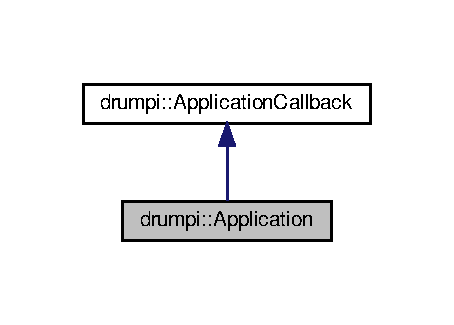
\includegraphics[width=218pt]{classdrumpi_1_1Application__inherit__graph}
\end{center}
\end{figure}


Collaboration diagram for drumpi\+:\+:Application\+:
\nopagebreak
\begin{figure}[H]
\begin{center}
\leavevmode
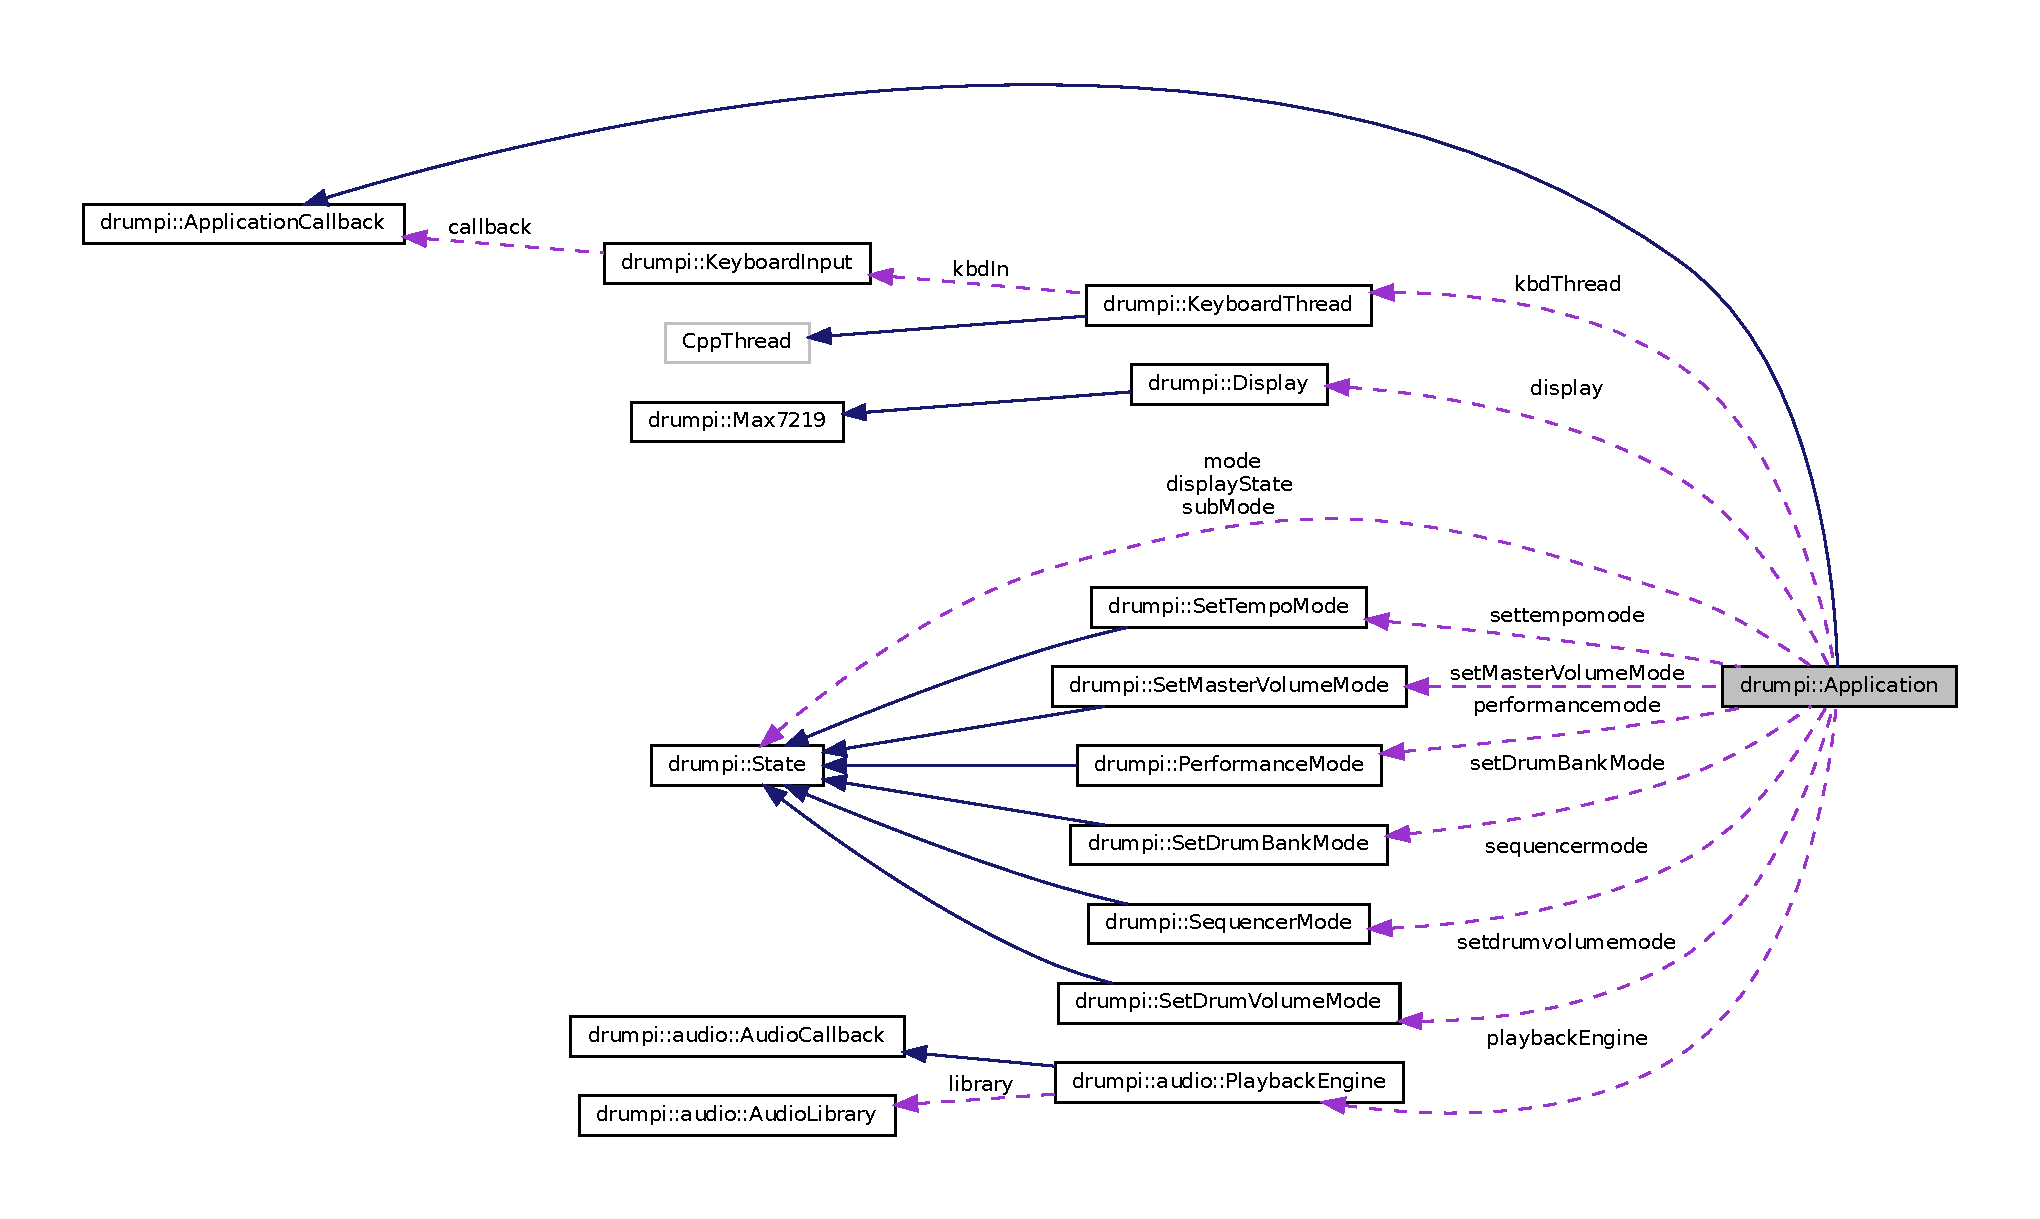
\includegraphics[width=350pt]{classdrumpi_1_1Application__coll__graph}
\end{center}
\end{figure}
\subsection*{Public Member Functions}
\begin{DoxyCompactItemize}
\item 
\hyperlink{classdrumpi_1_1Application_afa8cc05ce6b6092be5ecdfdae44e05f8}{Application} ()
\item 
void \hyperlink{classdrumpi_1_1Application_a31dd3f7f8fba9fc2fd32ceaff6ce36e7}{setup} ()
\begin{DoxyCompactList}\small\item\em Sets up the application. \end{DoxyCompactList}\item 
void \hyperlink{classdrumpi_1_1Application_a68965449404743bf1add056784d6cf81}{run} ()
\begin{DoxyCompactList}\small\item\em Runs the application. \end{DoxyCompactList}\item 
void \hyperlink{classdrumpi_1_1Application_af9f0221f37ccb5e324599554ac5ceadf}{interpret\+Key\+Press} (int key) override
\item 
void \hyperlink{classdrumpi_1_1Application_a39fcfaf7262d03c0c6824edcd552de4f}{set\+State} (\hyperlink{namespacedrumpi_af70ab0854d65f24f7fa353fdc1c46bc9}{state\+Label\+\_\+t} newstate) override
\end{DoxyCompactItemize}
\subsection*{Public Attributes}
\begin{DoxyCompactItemize}
\item 
\hyperlink{classdrumpi_1_1PerformanceMode}{Performance\+Mode} \hyperlink{classdrumpi_1_1Application_aa487db770d15b0fd9058954fdbe6389b}{performancemode}
\item 
\hyperlink{classdrumpi_1_1SequencerMode}{Sequencer\+Mode} \hyperlink{classdrumpi_1_1Application_a0e63d5d44014bd4bed1cdfd10f88bbf3}{sequencermode}
\item 
\hyperlink{classdrumpi_1_1State}{State} $\ast$ \hyperlink{classdrumpi_1_1Application_a12010a4072b841383566235a9ee4c20d}{mode}
\item 
\hyperlink{classdrumpi_1_1SetMasterVolumeMode}{Set\+Master\+Volume\+Mode} \hyperlink{classdrumpi_1_1Application_a9a6dfaebc7929553d6b1b5ed9407be11}{set\+Master\+Volume\+Mode}
\item 
\hyperlink{classdrumpi_1_1SetTempoMode}{Set\+Tempo\+Mode} \hyperlink{classdrumpi_1_1Application_a2316f62710a89af187fe7bec9fcac5e8}{settempomode}
\item 
\hyperlink{classdrumpi_1_1SetDrumVolumeMode}{Set\+Drum\+Volume\+Mode} \hyperlink{classdrumpi_1_1Application_a6993ce12d76456caba93f453da580892}{setdrumvolumemode}
\item 
\hyperlink{classdrumpi_1_1SetDrumBankMode}{Set\+Drum\+Bank\+Mode} \hyperlink{classdrumpi_1_1Application_a92e4162f1a85a267ff7de85ebeb31f8a}{set\+Drum\+Bank\+Mode}
\item 
\hyperlink{classdrumpi_1_1State}{State} $\ast$ \hyperlink{classdrumpi_1_1Application_a8af8346be9bf3ff5b3307336d0a9a406}{sub\+Mode}
\item 
\hyperlink{classdrumpi_1_1State}{State} $\ast$ \hyperlink{classdrumpi_1_1Application_a69da7a09674251d1d54b67c7ea915066}{display\+State}
\item 
\hyperlink{classdrumpi_1_1KeyboardThread}{Keyboard\+Thread} \hyperlink{classdrumpi_1_1Application_aace4b13db8cd738d2f3650fdd792f2e0}{kbd\+Thread}
\item 
std\+::unique\+\_\+ptr$<$ \hyperlink{classdrumpi_1_1audio_1_1JackClient}{audio\+::\+Jack\+Client} $>$ \hyperlink{classdrumpi_1_1Application_a9205c148fcc133669c08e8134dd3b151}{audio\+Engine} = nullptr
\item 
std\+::unique\+\_\+ptr$<$ \hyperlink{classdrumpi_1_1DisplayClock}{Display\+Clock} $>$ \hyperlink{classdrumpi_1_1Application_afaaa7672fa3f338283cf3b2c355272b0}{display\+Clock} = nullptr
\item 
std\+::unique\+\_\+ptr$<$ \hyperlink{classdrumpi_1_1DisplayDelay}{Display\+Delay} $>$ \hyperlink{classdrumpi_1_1Application_a86917e6bfed1be47bde5ea4929670d4b}{display\+Delay} = nullptr
\item 
\hyperlink{classdrumpi_1_1audio_1_1PlaybackEngine}{audio\+::\+Playback\+Engine} \hyperlink{classdrumpi_1_1Application_a813412b90daccbf979d7659224e0abee}{playback\+Engine}
\item 
\hyperlink{classdrumpi_1_1Display}{Display} \hyperlink{classdrumpi_1_1Application_ad318b1bdecc292bbbf3a91cf832dd97a}{display}
\item 
std\+::shared\+\_\+ptr$<$ \hyperlink{classdrumpi_1_1Sequencer}{Sequencer} $>$ \hyperlink{classdrumpi_1_1Application_ad795ecd7508c554e1f50183505ee052d}{seq} = nullptr
\item 
std\+::unique\+\_\+ptr$<$ \hyperlink{classdrumpi_1_1SequencerClock}{Sequencer\+Clock} $>$ \hyperlink{classdrumpi_1_1Application_a62b1dda72ffccc481b62a0c5b2ae9b84}{seq\+Clocker} = nullptr
\end{DoxyCompactItemize}


\subsection{Detailed Description}
Main application. 

This is the main application for the Drum\+Pi program. Its \hyperlink{classdrumpi_1_1Application_a31dd3f7f8fba9fc2fd32ceaff6ce36e7}{setup} and \hyperlink{classdrumpi_1_1Application_a68965449404743bf1add056784d6cf81}{run} methods are called when the application is started. 

\subsection{Constructor \& Destructor Documentation}
\mbox{\Hypertarget{classdrumpi_1_1Application_afa8cc05ce6b6092be5ecdfdae44e05f8}\label{classdrumpi_1_1Application_afa8cc05ce6b6092be5ecdfdae44e05f8}} 
\index{drumpi\+::\+Application@{drumpi\+::\+Application}!Application@{Application}}
\index{Application@{Application}!drumpi\+::\+Application@{drumpi\+::\+Application}}
\subsubsection{\texorpdfstring{Application()}{Application()}}
{\footnotesize\ttfamily Application\+::\+Application (\begin{DoxyParamCaption}{ }\end{DoxyParamCaption})}

Constructor 

\subsection{Member Function Documentation}
\mbox{\Hypertarget{classdrumpi_1_1Application_af9f0221f37ccb5e324599554ac5ceadf}\label{classdrumpi_1_1Application_af9f0221f37ccb5e324599554ac5ceadf}} 
\index{drumpi\+::\+Application@{drumpi\+::\+Application}!interpret\+Key\+Press@{interpret\+Key\+Press}}
\index{interpret\+Key\+Press@{interpret\+Key\+Press}!drumpi\+::\+Application@{drumpi\+::\+Application}}
\subsubsection{\texorpdfstring{interpret\+Key\+Press()}{interpretKeyPress()}}
{\footnotesize\ttfamily void Application\+::interpret\+Key\+Press (\begin{DoxyParamCaption}\item[{int}]{key }\end{DoxyParamCaption})\hspace{0.3cm}{\ttfamily [override]}, {\ttfamily [virtual]}}

This method is called by \hyperlink{classdrumpi_1_1KeyboardInput}{Keyboard\+Input} when a keyboard event occurs.


\begin{DoxyParams}{Parameters}
{\em key} & The keypress detected. \\
\hline
\end{DoxyParams}


Implements \hyperlink{classdrumpi_1_1ApplicationCallback_ab3f7606af20b435e8d2db240155c02d1}{drumpi\+::\+Application\+Callback}.

\mbox{\Hypertarget{classdrumpi_1_1Application_a68965449404743bf1add056784d6cf81}\label{classdrumpi_1_1Application_a68965449404743bf1add056784d6cf81}} 
\index{drumpi\+::\+Application@{drumpi\+::\+Application}!run@{run}}
\index{run@{run}!drumpi\+::\+Application@{drumpi\+::\+Application}}
\subsubsection{\texorpdfstring{run()}{run()}}
{\footnotesize\ttfamily void Application\+::run (\begin{DoxyParamCaption}{ }\end{DoxyParamCaption})}



Runs the application. 

This method is called on startup after setup has been performed, starting the audio engine, the display refresh clock, and creating the keyboard thread. \mbox{\Hypertarget{classdrumpi_1_1Application_a39fcfaf7262d03c0c6824edcd552de4f}\label{classdrumpi_1_1Application_a39fcfaf7262d03c0c6824edcd552de4f}} 
\index{drumpi\+::\+Application@{drumpi\+::\+Application}!set\+State@{set\+State}}
\index{set\+State@{set\+State}!drumpi\+::\+Application@{drumpi\+::\+Application}}
\subsubsection{\texorpdfstring{set\+State()}{setState()}}
{\footnotesize\ttfamily void Application\+::set\+State (\begin{DoxyParamCaption}\item[{\hyperlink{namespacedrumpi_af70ab0854d65f24f7fa353fdc1c46bc9}{state\+Label\+\_\+t}}]{newstate }\end{DoxyParamCaption})\hspace{0.3cm}{\ttfamily [override]}, {\ttfamily [virtual]}}

Changes the current state. 

Implements \hyperlink{classdrumpi_1_1ApplicationCallback_a009f5eb3ef1d4d3ee339ba3d1c6c52cf}{drumpi\+::\+Application\+Callback}.

\mbox{\Hypertarget{classdrumpi_1_1Application_a31dd3f7f8fba9fc2fd32ceaff6ce36e7}\label{classdrumpi_1_1Application_a31dd3f7f8fba9fc2fd32ceaff6ce36e7}} 
\index{drumpi\+::\+Application@{drumpi\+::\+Application}!setup@{setup}}
\index{setup@{setup}!drumpi\+::\+Application@{drumpi\+::\+Application}}
\subsubsection{\texorpdfstring{setup()}{setup()}}
{\footnotesize\ttfamily void Application\+::setup (\begin{DoxyParamCaption}{ }\end{DoxyParamCaption})}



Sets up the application. 

This method is called on startup to perform various set up tasks, including connecting the \hyperlink{classdrumpi_1_1Application}{Application} to the \hyperlink{classdrumpi_1_1KeyboardInput}{Keyboard\+Input} as a callback, resetting the sequencer and display, and loading the drum sample bank. 

\subsection{Member Data Documentation}
\mbox{\Hypertarget{classdrumpi_1_1Application_a9205c148fcc133669c08e8134dd3b151}\label{classdrumpi_1_1Application_a9205c148fcc133669c08e8134dd3b151}} 
\index{drumpi\+::\+Application@{drumpi\+::\+Application}!audio\+Engine@{audio\+Engine}}
\index{audio\+Engine@{audio\+Engine}!drumpi\+::\+Application@{drumpi\+::\+Application}}
\subsubsection{\texorpdfstring{audio\+Engine}{audioEngine}}
{\footnotesize\ttfamily std\+::unique\+\_\+ptr$<$\hyperlink{classdrumpi_1_1audio_1_1JackClient}{audio\+::\+Jack\+Client}$>$ drumpi\+::\+Application\+::audio\+Engine = nullptr}

Audio\+Engine object. \mbox{\Hypertarget{classdrumpi_1_1Application_ad318b1bdecc292bbbf3a91cf832dd97a}\label{classdrumpi_1_1Application_ad318b1bdecc292bbbf3a91cf832dd97a}} 
\index{drumpi\+::\+Application@{drumpi\+::\+Application}!display@{display}}
\index{display@{display}!drumpi\+::\+Application@{drumpi\+::\+Application}}
\subsubsection{\texorpdfstring{display}{display}}
{\footnotesize\ttfamily \hyperlink{classdrumpi_1_1Display}{Display} drumpi\+::\+Application\+::display}

\hyperlink{classdrumpi_1_1Display}{Display} object. \mbox{\Hypertarget{classdrumpi_1_1Application_afaaa7672fa3f338283cf3b2c355272b0}\label{classdrumpi_1_1Application_afaaa7672fa3f338283cf3b2c355272b0}} 
\index{drumpi\+::\+Application@{drumpi\+::\+Application}!display\+Clock@{display\+Clock}}
\index{display\+Clock@{display\+Clock}!drumpi\+::\+Application@{drumpi\+::\+Application}}
\subsubsection{\texorpdfstring{display\+Clock}{displayClock}}
{\footnotesize\ttfamily std\+::unique\+\_\+ptr$<$\hyperlink{classdrumpi_1_1DisplayClock}{Display\+Clock}$>$ drumpi\+::\+Application\+::display\+Clock = nullptr}

\hyperlink{classdrumpi_1_1DisplayClock}{Display\+Clock} object. \mbox{\Hypertarget{classdrumpi_1_1Application_a86917e6bfed1be47bde5ea4929670d4b}\label{classdrumpi_1_1Application_a86917e6bfed1be47bde5ea4929670d4b}} 
\index{drumpi\+::\+Application@{drumpi\+::\+Application}!display\+Delay@{display\+Delay}}
\index{display\+Delay@{display\+Delay}!drumpi\+::\+Application@{drumpi\+::\+Application}}
\subsubsection{\texorpdfstring{display\+Delay}{displayDelay}}
{\footnotesize\ttfamily std\+::unique\+\_\+ptr$<$\hyperlink{classdrumpi_1_1DisplayDelay}{Display\+Delay}$>$ drumpi\+::\+Application\+::display\+Delay = nullptr}

Display\+Timer object. \mbox{\Hypertarget{classdrumpi_1_1Application_a69da7a09674251d1d54b67c7ea915066}\label{classdrumpi_1_1Application_a69da7a09674251d1d54b67c7ea915066}} 
\index{drumpi\+::\+Application@{drumpi\+::\+Application}!display\+State@{display\+State}}
\index{display\+State@{display\+State}!drumpi\+::\+Application@{drumpi\+::\+Application}}
\subsubsection{\texorpdfstring{display\+State}{displayState}}
{\footnotesize\ttfamily \hyperlink{classdrumpi_1_1State}{State}$\ast$ drumpi\+::\+Application\+::display\+State}

Pointer to the state to be displayed. \mbox{\Hypertarget{classdrumpi_1_1Application_aace4b13db8cd738d2f3650fdd792f2e0}\label{classdrumpi_1_1Application_aace4b13db8cd738d2f3650fdd792f2e0}} 
\index{drumpi\+::\+Application@{drumpi\+::\+Application}!kbd\+Thread@{kbd\+Thread}}
\index{kbd\+Thread@{kbd\+Thread}!drumpi\+::\+Application@{drumpi\+::\+Application}}
\subsubsection{\texorpdfstring{kbd\+Thread}{kbdThread}}
{\footnotesize\ttfamily \hyperlink{classdrumpi_1_1KeyboardThread}{Keyboard\+Thread} drumpi\+::\+Application\+::kbd\+Thread}

Instance of \hyperlink{classdrumpi_1_1KeyboardThread}{Keyboard\+Thread} class. \mbox{\Hypertarget{classdrumpi_1_1Application_a12010a4072b841383566235a9ee4c20d}\label{classdrumpi_1_1Application_a12010a4072b841383566235a9ee4c20d}} 
\index{drumpi\+::\+Application@{drumpi\+::\+Application}!mode@{mode}}
\index{mode@{mode}!drumpi\+::\+Application@{drumpi\+::\+Application}}
\subsubsection{\texorpdfstring{mode}{mode}}
{\footnotesize\ttfamily \hyperlink{classdrumpi_1_1State}{State}$\ast$ drumpi\+::\+Application\+::mode}

Pointer to the current mode instance. \mbox{\Hypertarget{classdrumpi_1_1Application_aa487db770d15b0fd9058954fdbe6389b}\label{classdrumpi_1_1Application_aa487db770d15b0fd9058954fdbe6389b}} 
\index{drumpi\+::\+Application@{drumpi\+::\+Application}!performancemode@{performancemode}}
\index{performancemode@{performancemode}!drumpi\+::\+Application@{drumpi\+::\+Application}}
\subsubsection{\texorpdfstring{performancemode}{performancemode}}
{\footnotesize\ttfamily \hyperlink{classdrumpi_1_1PerformanceMode}{Performance\+Mode} drumpi\+::\+Application\+::performancemode}

Instance of \hyperlink{classdrumpi_1_1PerformanceMode}{Performance\+Mode} state. \mbox{\Hypertarget{classdrumpi_1_1Application_a813412b90daccbf979d7659224e0abee}\label{classdrumpi_1_1Application_a813412b90daccbf979d7659224e0abee}} 
\index{drumpi\+::\+Application@{drumpi\+::\+Application}!playback\+Engine@{playback\+Engine}}
\index{playback\+Engine@{playback\+Engine}!drumpi\+::\+Application@{drumpi\+::\+Application}}
\subsubsection{\texorpdfstring{playback\+Engine}{playbackEngine}}
{\footnotesize\ttfamily \hyperlink{classdrumpi_1_1audio_1_1PlaybackEngine}{audio\+::\+Playback\+Engine} drumpi\+::\+Application\+::playback\+Engine}

Playback\+Engine object. \mbox{\Hypertarget{classdrumpi_1_1Application_ad795ecd7508c554e1f50183505ee052d}\label{classdrumpi_1_1Application_ad795ecd7508c554e1f50183505ee052d}} 
\index{drumpi\+::\+Application@{drumpi\+::\+Application}!seq@{seq}}
\index{seq@{seq}!drumpi\+::\+Application@{drumpi\+::\+Application}}
\subsubsection{\texorpdfstring{seq}{seq}}
{\footnotesize\ttfamily std\+::shared\+\_\+ptr$<$\hyperlink{classdrumpi_1_1Sequencer}{Sequencer}$>$ drumpi\+::\+Application\+::seq = nullptr}

\hyperlink{classdrumpi_1_1Sequencer}{Sequencer} object. \mbox{\Hypertarget{classdrumpi_1_1Application_a62b1dda72ffccc481b62a0c5b2ae9b84}\label{classdrumpi_1_1Application_a62b1dda72ffccc481b62a0c5b2ae9b84}} 
\index{drumpi\+::\+Application@{drumpi\+::\+Application}!seq\+Clocker@{seq\+Clocker}}
\index{seq\+Clocker@{seq\+Clocker}!drumpi\+::\+Application@{drumpi\+::\+Application}}
\subsubsection{\texorpdfstring{seq\+Clocker}{seqClocker}}
{\footnotesize\ttfamily std\+::unique\+\_\+ptr$<$\hyperlink{classdrumpi_1_1SequencerClock}{Sequencer\+Clock}$>$ drumpi\+::\+Application\+::seq\+Clocker = nullptr}

\hyperlink{classdrumpi_1_1SequencerClock}{Sequencer\+Clock} object used to clock the \hyperlink{classdrumpi_1_1Sequencer}{Sequencer}. \mbox{\Hypertarget{classdrumpi_1_1Application_a0e63d5d44014bd4bed1cdfd10f88bbf3}\label{classdrumpi_1_1Application_a0e63d5d44014bd4bed1cdfd10f88bbf3}} 
\index{drumpi\+::\+Application@{drumpi\+::\+Application}!sequencermode@{sequencermode}}
\index{sequencermode@{sequencermode}!drumpi\+::\+Application@{drumpi\+::\+Application}}
\subsubsection{\texorpdfstring{sequencermode}{sequencermode}}
{\footnotesize\ttfamily \hyperlink{classdrumpi_1_1SequencerMode}{Sequencer\+Mode} drumpi\+::\+Application\+::sequencermode}

Instance of \hyperlink{classdrumpi_1_1SequencerMode}{Sequencer\+Mode} state. \mbox{\Hypertarget{classdrumpi_1_1Application_a92e4162f1a85a267ff7de85ebeb31f8a}\label{classdrumpi_1_1Application_a92e4162f1a85a267ff7de85ebeb31f8a}} 
\index{drumpi\+::\+Application@{drumpi\+::\+Application}!set\+Drum\+Bank\+Mode@{set\+Drum\+Bank\+Mode}}
\index{set\+Drum\+Bank\+Mode@{set\+Drum\+Bank\+Mode}!drumpi\+::\+Application@{drumpi\+::\+Application}}
\subsubsection{\texorpdfstring{set\+Drum\+Bank\+Mode}{setDrumBankMode}}
{\footnotesize\ttfamily \hyperlink{classdrumpi_1_1SetDrumBankMode}{Set\+Drum\+Bank\+Mode} drumpi\+::\+Application\+::set\+Drum\+Bank\+Mode}

Instance of \hyperlink{classdrumpi_1_1SetDrumBankMode}{Set\+Drum\+Bank\+Mode} state. \mbox{\Hypertarget{classdrumpi_1_1Application_a6993ce12d76456caba93f453da580892}\label{classdrumpi_1_1Application_a6993ce12d76456caba93f453da580892}} 
\index{drumpi\+::\+Application@{drumpi\+::\+Application}!setdrumvolumemode@{setdrumvolumemode}}
\index{setdrumvolumemode@{setdrumvolumemode}!drumpi\+::\+Application@{drumpi\+::\+Application}}
\subsubsection{\texorpdfstring{setdrumvolumemode}{setdrumvolumemode}}
{\footnotesize\ttfamily \hyperlink{classdrumpi_1_1SetDrumVolumeMode}{Set\+Drum\+Volume\+Mode} drumpi\+::\+Application\+::setdrumvolumemode}

Instance of \hyperlink{classdrumpi_1_1SetDrumVolumeMode}{Set\+Drum\+Volume\+Mode} state. \mbox{\Hypertarget{classdrumpi_1_1Application_a9a6dfaebc7929553d6b1b5ed9407be11}\label{classdrumpi_1_1Application_a9a6dfaebc7929553d6b1b5ed9407be11}} 
\index{drumpi\+::\+Application@{drumpi\+::\+Application}!set\+Master\+Volume\+Mode@{set\+Master\+Volume\+Mode}}
\index{set\+Master\+Volume\+Mode@{set\+Master\+Volume\+Mode}!drumpi\+::\+Application@{drumpi\+::\+Application}}
\subsubsection{\texorpdfstring{set\+Master\+Volume\+Mode}{setMasterVolumeMode}}
{\footnotesize\ttfamily \hyperlink{classdrumpi_1_1SetMasterVolumeMode}{Set\+Master\+Volume\+Mode} drumpi\+::\+Application\+::set\+Master\+Volume\+Mode}

Instance of \hyperlink{classdrumpi_1_1SetMasterVolumeMode}{Set\+Master\+Volume\+Mode} state. \mbox{\Hypertarget{classdrumpi_1_1Application_a2316f62710a89af187fe7bec9fcac5e8}\label{classdrumpi_1_1Application_a2316f62710a89af187fe7bec9fcac5e8}} 
\index{drumpi\+::\+Application@{drumpi\+::\+Application}!settempomode@{settempomode}}
\index{settempomode@{settempomode}!drumpi\+::\+Application@{drumpi\+::\+Application}}
\subsubsection{\texorpdfstring{settempomode}{settempomode}}
{\footnotesize\ttfamily \hyperlink{classdrumpi_1_1SetTempoMode}{Set\+Tempo\+Mode} drumpi\+::\+Application\+::settempomode}

Instance of \hyperlink{classdrumpi_1_1SetTempoMode}{Set\+Tempo\+Mode} state. \mbox{\Hypertarget{classdrumpi_1_1Application_a8af8346be9bf3ff5b3307336d0a9a406}\label{classdrumpi_1_1Application_a8af8346be9bf3ff5b3307336d0a9a406}} 
\index{drumpi\+::\+Application@{drumpi\+::\+Application}!sub\+Mode@{sub\+Mode}}
\index{sub\+Mode@{sub\+Mode}!drumpi\+::\+Application@{drumpi\+::\+Application}}
\subsubsection{\texorpdfstring{sub\+Mode}{subMode}}
{\footnotesize\ttfamily \hyperlink{classdrumpi_1_1State}{State}$\ast$ drumpi\+::\+Application\+::sub\+Mode}

Pointer to the current sub-\/mode instance. 

The documentation for this class was generated from the following files\+:\begin{DoxyCompactItemize}
\item 
src/application.\+hpp\item 
src/application.\+cpp\end{DoxyCompactItemize}

\hypertarget{classdrumpi_1_1ApplicationCallback}{}\doxysection{drumpi\+::Application\+Callback Class Reference}
\label{classdrumpi_1_1ApplicationCallback}\index{drumpi::ApplicationCallback@{drumpi::ApplicationCallback}}


{\ttfamily \#include $<$applicationcallback.\+hpp$>$}



Inheritance diagram for drumpi\+::Application\+Callback\+:
\nopagebreak
\begin{figure}[H]
\begin{center}
\leavevmode
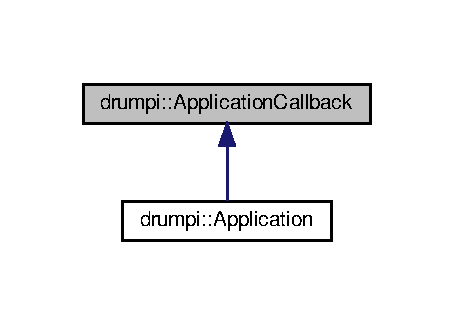
\includegraphics[width=234pt]{classdrumpi_1_1ApplicationCallback__inherit__graph}
\end{center}
\end{figure}
\doxysubsection*{Public Member Functions}
\begin{DoxyCompactItemize}
\item 
virtual void \mbox{\hyperlink{classdrumpi_1_1ApplicationCallback_ab3f7606af20b435e8d2db240155c02d1}{interpret\+Key\+Press}} (int key)=0
\item 
virtual void \mbox{\hyperlink{classdrumpi_1_1ApplicationCallback_a009f5eb3ef1d4d3ee339ba3d1c6c52cf}{set\+State}} (\mbox{\hyperlink{namespacedrumpi_ae7f2b32a0392a4c469ce4dc84a64e845}{state\+Label\+\_\+t}} newstate)=0
\end{DoxyCompactItemize}
\doxysubsection*{Public Attributes}
\begin{DoxyCompactItemize}
\item 
bool \mbox{\hyperlink{classdrumpi_1_1ApplicationCallback_a2de8dc466288bf85770cf58422eecc1c}{running}}
\end{DoxyCompactItemize}


\doxysubsection{Detailed Description}
Abstract application callback class. 

\doxysubsection{Member Function Documentation}
\mbox{\Hypertarget{classdrumpi_1_1ApplicationCallback_ab3f7606af20b435e8d2db240155c02d1}\label{classdrumpi_1_1ApplicationCallback_ab3f7606af20b435e8d2db240155c02d1}} 
\index{drumpi::ApplicationCallback@{drumpi::ApplicationCallback}!interpretKeyPress@{interpretKeyPress}}
\index{interpretKeyPress@{interpretKeyPress}!drumpi::ApplicationCallback@{drumpi::ApplicationCallback}}
\doxysubsubsection{\texorpdfstring{interpretKeyPress()}{interpretKeyPress()}}
{\footnotesize\ttfamily virtual void drumpi\+::\+Application\+Callback\+::interpret\+Key\+Press (\begin{DoxyParamCaption}\item[{int}]{key }\end{DoxyParamCaption})\hspace{0.3cm}{\ttfamily [pure virtual]}}

Virtual function to be overridden by derived class. 

Implemented in \mbox{\hyperlink{classdrumpi_1_1Application_af9f0221f37ccb5e324599554ac5ceadf}{drumpi\+::\+Application}}.

\mbox{\Hypertarget{classdrumpi_1_1ApplicationCallback_a009f5eb3ef1d4d3ee339ba3d1c6c52cf}\label{classdrumpi_1_1ApplicationCallback_a009f5eb3ef1d4d3ee339ba3d1c6c52cf}} 
\index{drumpi::ApplicationCallback@{drumpi::ApplicationCallback}!setState@{setState}}
\index{setState@{setState}!drumpi::ApplicationCallback@{drumpi::ApplicationCallback}}
\doxysubsubsection{\texorpdfstring{setState()}{setState()}}
{\footnotesize\ttfamily virtual void drumpi\+::\+Application\+Callback\+::set\+State (\begin{DoxyParamCaption}\item[{\mbox{\hyperlink{namespacedrumpi_ae7f2b32a0392a4c469ce4dc84a64e845}{state\+Label\+\_\+t}}}]{newstate }\end{DoxyParamCaption})\hspace{0.3cm}{\ttfamily [pure virtual]}}

Virtual function to be overridden by derived class. 

Implemented in \mbox{\hyperlink{classdrumpi_1_1Application_a39fcfaf7262d03c0c6824edcd552de4f}{drumpi\+::\+Application}}.



\doxysubsection{Member Data Documentation}
\mbox{\Hypertarget{classdrumpi_1_1ApplicationCallback_a2de8dc466288bf85770cf58422eecc1c}\label{classdrumpi_1_1ApplicationCallback_a2de8dc466288bf85770cf58422eecc1c}} 
\index{drumpi::ApplicationCallback@{drumpi::ApplicationCallback}!running@{running}}
\index{running@{running}!drumpi::ApplicationCallback@{drumpi::ApplicationCallback}}
\doxysubsubsection{\texorpdfstring{running}{running}}
{\footnotesize\ttfamily bool drumpi\+::\+Application\+Callback\+::running}

Running flag for the application. 

The documentation for this class was generated from the following file\+:\begin{DoxyCompactItemize}
\item 
src/applicationcallback.\+hpp\end{DoxyCompactItemize}

\hypertarget{classdrumpi_1_1audio_1_1AudioCallback}{}\doxysection{drumpi\+::audio\+::Audio\+Callback Class Reference}
\label{classdrumpi_1_1audio_1_1AudioCallback}\index{drumpi::audio::AudioCallback@{drumpi::audio::AudioCallback}}


{\ttfamily \#include $<$audio.\+hpp$>$}



Inheritance diagram for drumpi\+::audio\+::Audio\+Callback\+:\nopagebreak
\begin{figure}[H]
\begin{center}
\leavevmode
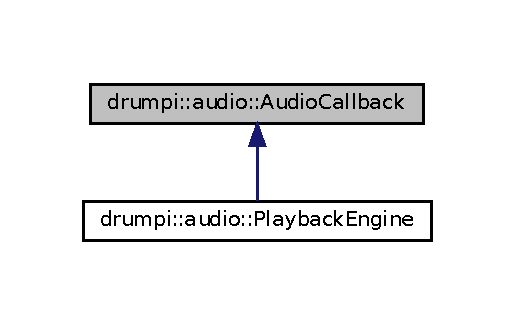
\includegraphics[width=247pt]{classdrumpi_1_1audio_1_1AudioCallback__inherit__graph}
\end{center}
\end{figure}
\doxysubsection*{Public Member Functions}
\begin{DoxyCompactItemize}
\item 
virtual std\+::vector$<$ \mbox{\hyperlink{namespacedrumpi_1_1audio_aca0bdc9164f87b72057e284442abab6e}{sample\+\_\+t}} $>$ \mbox{\hyperlink{classdrumpi_1_1audio_1_1AudioCallback_a9f53a830e6fd3d8eecf6f6ebb27314cd}{get\+Samples}} (int n\+Samples)=0
\end{DoxyCompactItemize}


\doxysubsection{Detailed Description}
Abstract sample retieval callback class. 

\doxysubsection{Member Function Documentation}
\mbox{\Hypertarget{classdrumpi_1_1audio_1_1AudioCallback_a9f53a830e6fd3d8eecf6f6ebb27314cd}\label{classdrumpi_1_1audio_1_1AudioCallback_a9f53a830e6fd3d8eecf6f6ebb27314cd}} 
\index{drumpi::audio::AudioCallback@{drumpi::audio::AudioCallback}!getSamples@{getSamples}}
\index{getSamples@{getSamples}!drumpi::audio::AudioCallback@{drumpi::audio::AudioCallback}}
\doxysubsubsection{\texorpdfstring{getSamples()}{getSamples()}}
{\footnotesize\ttfamily virtual std\+::vector$<$\mbox{\hyperlink{namespacedrumpi_1_1audio_aca0bdc9164f87b72057e284442abab6e}{sample\+\_\+t}}$>$ drumpi\+::audio\+::\+Audio\+Callback\+::get\+Samples (\begin{DoxyParamCaption}\item[{int}]{n\+Samples }\end{DoxyParamCaption})\hspace{0.3cm}{\ttfamily [pure virtual]}}

Called by a \mbox{\hyperlink{classdrumpi_1_1audio_1_1JackClient}{Jack\+Client}} object when samples are requested by Jack. 
\begin{DoxyParams}{Parameters}
{\em n\+Samples} & the number of samples requested. \\
\hline
\end{DoxyParams}
\begin{DoxyReturn}{Returns}
a vector of samples, of type \mbox{\hyperlink{namespacedrumpi_1_1audio_aca0bdc9164f87b72057e284442abab6e}{sample\+\_\+t}} ({\ttfamily float}) 
\end{DoxyReturn}


Implemented in \mbox{\hyperlink{classdrumpi_1_1audio_1_1PlaybackEngine_a16f4d8c36323b3b580475cd5fc4421c2}{drumpi\+::audio\+::\+Playback\+Engine}}.



The documentation for this class was generated from the following file\+:\begin{DoxyCompactItemize}
\item 
src/audio.\+hpp\end{DoxyCompactItemize}

\hypertarget{classdrumpi_1_1audio_1_1AudioClip}{}\doxysection{drumpi\+::audio\+::Audio\+Clip Class Reference}
\label{classdrumpi_1_1audio_1_1AudioClip}\index{drumpi::audio::AudioClip@{drumpi::audio::AudioClip}}


{\ttfamily \#include $<$sample\+Source.\+hpp$>$}



Inheritance diagram for drumpi\+::audio\+::Audio\+Clip\+:\nopagebreak
\begin{figure}[H]
\begin{center}
\leavevmode
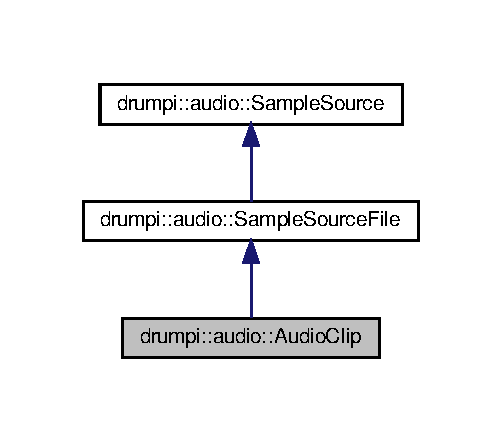
\includegraphics[width=257pt]{classdrumpi_1_1audio_1_1AudioClip__inherit__graph}
\end{center}
\end{figure}


Collaboration diagram for drumpi\+::audio\+::Audio\+Clip\+:\nopagebreak
\begin{figure}[H]
\begin{center}
\leavevmode
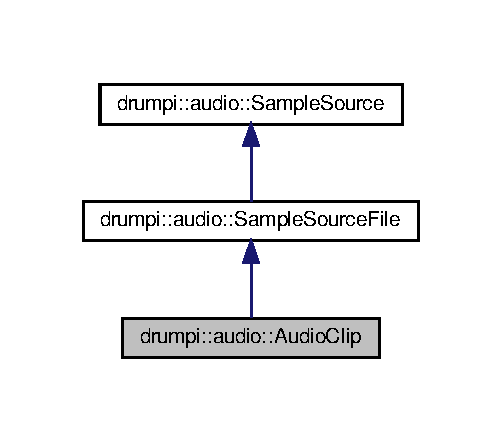
\includegraphics[width=257pt]{classdrumpi_1_1audio_1_1AudioClip__coll__graph}
\end{center}
\end{figure}
\doxysubsection*{Public Member Functions}
\begin{DoxyCompactItemize}
\item 
\mbox{\hyperlink{classdrumpi_1_1audio_1_1AudioClip_aec77804b78d89a21cb789b80a013c4fc}{Audio\+Clip}} (std\+::string \mbox{\hyperlink{classdrumpi_1_1audio_1_1SampleSourceFile_a0d6461310f720bf9a25e7c274f57053b}{filepath}})
\item 
std\+::vector$<$ \mbox{\hyperlink{namespacedrumpi_1_1audio_aca0bdc9164f87b72057e284442abab6e}{sample\+\_\+t}} $>$ \mbox{\hyperlink{classdrumpi_1_1audio_1_1AudioClip_aad8e2b4282047c0fb884d4f93210c83b}{get\+Samples}} (int n\+Samples) override
\item 
void \mbox{\hyperlink{classdrumpi_1_1audio_1_1AudioClip_ac870bf37050afae302754c4e4671d779}{reset}} () override
\item 
void \mbox{\hyperlink{classdrumpi_1_1audio_1_1AudioClip_aeed08721b08d9443a769a99e717f5743}{update\+Status}} () override
\item 
void \mbox{\hyperlink{classdrumpi_1_1audio_1_1AudioClip_a9696d29532e37f6ea04c6353f0e3748b}{hard\+Reset}} ()
\end{DoxyCompactItemize}
\doxysubsection*{Private Member Functions}
\begin{DoxyCompactItemize}
\item 
void \mbox{\hyperlink{classdrumpi_1_1audio_1_1AudioClip_af00b5d353bec63b6bbbbe58509b95fe3}{load\+File}} (std\+::string \mbox{\hyperlink{classdrumpi_1_1audio_1_1SampleSourceFile_a0d6461310f720bf9a25e7c274f57053b}{filepath}}) override
\item 
int \mbox{\hyperlink{classdrumpi_1_1audio_1_1AudioClip_a04519734485d53672fe56ddac590b428}{samples\+Remaining}} ()
\end{DoxyCompactItemize}
\doxysubsection*{Private Attributes}
\begin{DoxyCompactItemize}
\item 
std\+::vector$<$ \mbox{\hyperlink{namespacedrumpi_1_1audio_aca0bdc9164f87b72057e284442abab6e}{sample\+\_\+t}} $>$ \mbox{\hyperlink{classdrumpi_1_1audio_1_1AudioClip_a3d99c707ac474917167a9936e09e620a}{clip}}
\item 
int \mbox{\hyperlink{classdrumpi_1_1audio_1_1AudioClip_a5ee7a6ff9e98c5c3f72ec72405d96e58}{num\+Samples}}
\item 
int \mbox{\hyperlink{classdrumpi_1_1audio_1_1AudioClip_ad901741b22d0efe60079054cb572f6f5}{playhead}}
\end{DoxyCompactItemize}
\doxysubsection*{Additional Inherited Members}


\doxysubsection{Detailed Description}
Handler class for pre-\/generated drum samples. 

\doxysubsection{Constructor \& Destructor Documentation}
\mbox{\Hypertarget{classdrumpi_1_1audio_1_1AudioClip_aec77804b78d89a21cb789b80a013c4fc}\label{classdrumpi_1_1audio_1_1AudioClip_aec77804b78d89a21cb789b80a013c4fc}} 
\index{drumpi::audio::AudioClip@{drumpi::audio::AudioClip}!AudioClip@{AudioClip}}
\index{AudioClip@{AudioClip}!drumpi::audio::AudioClip@{drumpi::audio::AudioClip}}
\doxysubsubsection{\texorpdfstring{AudioClip()}{AudioClip()}}
{\footnotesize\ttfamily Audio\+Clip\+::\+Audio\+Clip (\begin{DoxyParamCaption}\item[{std\+::string}]{filepath }\end{DoxyParamCaption})}

Class constructor. 
\begin{DoxyParams}{Parameters}
{\em filepath} & the absolute file path of an audio file. \\
\hline
\end{DoxyParams}


\doxysubsection{Member Function Documentation}
\mbox{\Hypertarget{classdrumpi_1_1audio_1_1AudioClip_aad8e2b4282047c0fb884d4f93210c83b}\label{classdrumpi_1_1audio_1_1AudioClip_aad8e2b4282047c0fb884d4f93210c83b}} 
\index{drumpi::audio::AudioClip@{drumpi::audio::AudioClip}!getSamples@{getSamples}}
\index{getSamples@{getSamples}!drumpi::audio::AudioClip@{drumpi::audio::AudioClip}}
\doxysubsubsection{\texorpdfstring{getSamples()}{getSamples()}}
{\footnotesize\ttfamily std\+::vector$<$ \mbox{\hyperlink{namespacedrumpi_1_1audio_aca0bdc9164f87b72057e284442abab6e}{sample\+\_\+t}} $>$ Audio\+Clip\+::get\+Samples (\begin{DoxyParamCaption}\item[{int}]{n\+Samples }\end{DoxyParamCaption})\hspace{0.3cm}{\ttfamily [override]}, {\ttfamily [virtual]}}

Returns a buffer of samples. 
\begin{DoxyParams}{Parameters}
{\em n\+Samples} & number of samples to be returned. \\
\hline
\end{DoxyParams}
\begin{DoxyReturn}{Returns}
a sample buffer of length n\+Samples. 
\end{DoxyReturn}


Implements \mbox{\hyperlink{classdrumpi_1_1audio_1_1SampleSource_ab3f12884325b818ebe088dec5daa15cd}{drumpi\+::audio\+::\+Sample\+Source}}.

\mbox{\Hypertarget{classdrumpi_1_1audio_1_1AudioClip_a9696d29532e37f6ea04c6353f0e3748b}\label{classdrumpi_1_1audio_1_1AudioClip_a9696d29532e37f6ea04c6353f0e3748b}} 
\index{drumpi::audio::AudioClip@{drumpi::audio::AudioClip}!hardReset@{hardReset}}
\index{hardReset@{hardReset}!drumpi::audio::AudioClip@{drumpi::audio::AudioClip}}
\doxysubsubsection{\texorpdfstring{hardReset()}{hardReset()}}
{\footnotesize\ttfamily void Audio\+Clip\+::hard\+Reset (\begin{DoxyParamCaption}{ }\end{DoxyParamCaption})}

Like \mbox{\hyperlink{classdrumpi_1_1audio_1_1AudioClip_ac870bf37050afae302754c4e4671d779}{reset}} but the clip is completely re-\/loaded. Not recommended for real-\/time use, but may be useful to recover from errors. \mbox{\Hypertarget{classdrumpi_1_1audio_1_1AudioClip_af00b5d353bec63b6bbbbe58509b95fe3}\label{classdrumpi_1_1audio_1_1AudioClip_af00b5d353bec63b6bbbbe58509b95fe3}} 
\index{drumpi::audio::AudioClip@{drumpi::audio::AudioClip}!loadFile@{loadFile}}
\index{loadFile@{loadFile}!drumpi::audio::AudioClip@{drumpi::audio::AudioClip}}
\doxysubsubsection{\texorpdfstring{loadFile()}{loadFile()}}
{\footnotesize\ttfamily void Audio\+Clip\+::load\+File (\begin{DoxyParamCaption}\item[{std\+::string}]{filepath }\end{DoxyParamCaption})\hspace{0.3cm}{\ttfamily [override]}, {\ttfamily [private]}, {\ttfamily [virtual]}}

Loads the specified file. 
\begin{DoxyParams}{Parameters}
{\em filepath} & file path of the file to load. \\
\hline
\end{DoxyParams}


Implements \mbox{\hyperlink{classdrumpi_1_1audio_1_1SampleSourceFile_a3a919325368cd163435f5ea6ad9fd4ec}{drumpi\+::audio\+::\+Sample\+Source\+File}}.

\mbox{\Hypertarget{classdrumpi_1_1audio_1_1AudioClip_ac870bf37050afae302754c4e4671d779}\label{classdrumpi_1_1audio_1_1AudioClip_ac870bf37050afae302754c4e4671d779}} 
\index{drumpi::audio::AudioClip@{drumpi::audio::AudioClip}!reset@{reset}}
\index{reset@{reset}!drumpi::audio::AudioClip@{drumpi::audio::AudioClip}}
\doxysubsubsection{\texorpdfstring{reset()}{reset()}}
{\footnotesize\ttfamily void Audio\+Clip\+::reset (\begin{DoxyParamCaption}{ }\end{DoxyParamCaption})\hspace{0.3cm}{\ttfamily [override]}, {\ttfamily [virtual]}}

Halts playback and returns playhead to start of clip. 

Implements \mbox{\hyperlink{classdrumpi_1_1audio_1_1SampleSource_aa7b214c99ee55ceac758fdef44b0cd6d}{drumpi\+::audio\+::\+Sample\+Source}}.

\mbox{\Hypertarget{classdrumpi_1_1audio_1_1AudioClip_a04519734485d53672fe56ddac590b428}\label{classdrumpi_1_1audio_1_1AudioClip_a04519734485d53672fe56ddac590b428}} 
\index{drumpi::audio::AudioClip@{drumpi::audio::AudioClip}!samplesRemaining@{samplesRemaining}}
\index{samplesRemaining@{samplesRemaining}!drumpi::audio::AudioClip@{drumpi::audio::AudioClip}}
\doxysubsubsection{\texorpdfstring{samplesRemaining()}{samplesRemaining()}}
{\footnotesize\ttfamily int Audio\+Clip\+::samples\+Remaining (\begin{DoxyParamCaption}{ }\end{DoxyParamCaption})\hspace{0.3cm}{\ttfamily [private]}}

Calculates the number of samples remaining for output. \mbox{\Hypertarget{classdrumpi_1_1audio_1_1AudioClip_aeed08721b08d9443a769a99e717f5743}\label{classdrumpi_1_1audio_1_1AudioClip_aeed08721b08d9443a769a99e717f5743}} 
\index{drumpi::audio::AudioClip@{drumpi::audio::AudioClip}!updateStatus@{updateStatus}}
\index{updateStatus@{updateStatus}!drumpi::audio::AudioClip@{drumpi::audio::AudioClip}}
\doxysubsubsection{\texorpdfstring{updateStatus()}{updateStatus()}}
{\footnotesize\ttfamily void Audio\+Clip\+::update\+Status (\begin{DoxyParamCaption}{ }\end{DoxyParamCaption})\hspace{0.3cm}{\ttfamily [override]}, {\ttfamily [virtual]}}

Updates the status of the source. 

Implements \mbox{\hyperlink{classdrumpi_1_1audio_1_1SampleSource_aff9beb7031bc5af424dccc525be5e9d3}{drumpi\+::audio\+::\+Sample\+Source}}.



\doxysubsection{Member Data Documentation}
\mbox{\Hypertarget{classdrumpi_1_1audio_1_1AudioClip_a3d99c707ac474917167a9936e09e620a}\label{classdrumpi_1_1audio_1_1AudioClip_a3d99c707ac474917167a9936e09e620a}} 
\index{drumpi::audio::AudioClip@{drumpi::audio::AudioClip}!clip@{clip}}
\index{clip@{clip}!drumpi::audio::AudioClip@{drumpi::audio::AudioClip}}
\doxysubsubsection{\texorpdfstring{clip}{clip}}
{\footnotesize\ttfamily std\+::vector$<$\mbox{\hyperlink{namespacedrumpi_1_1audio_aca0bdc9164f87b72057e284442abab6e}{sample\+\_\+t}}$>$ drumpi\+::audio\+::\+Audio\+Clip\+::clip\hspace{0.3cm}{\ttfamily [private]}}

Container for the audio clip. \mbox{\Hypertarget{classdrumpi_1_1audio_1_1AudioClip_a5ee7a6ff9e98c5c3f72ec72405d96e58}\label{classdrumpi_1_1audio_1_1AudioClip_a5ee7a6ff9e98c5c3f72ec72405d96e58}} 
\index{drumpi::audio::AudioClip@{drumpi::audio::AudioClip}!numSamples@{numSamples}}
\index{numSamples@{numSamples}!drumpi::audio::AudioClip@{drumpi::audio::AudioClip}}
\doxysubsubsection{\texorpdfstring{numSamples}{numSamples}}
{\footnotesize\ttfamily int drumpi\+::audio\+::\+Audio\+Clip\+::num\+Samples\hspace{0.3cm}{\ttfamily [private]}}

Number of samples in the audio clip. \mbox{\Hypertarget{classdrumpi_1_1audio_1_1AudioClip_ad901741b22d0efe60079054cb572f6f5}\label{classdrumpi_1_1audio_1_1AudioClip_ad901741b22d0efe60079054cb572f6f5}} 
\index{drumpi::audio::AudioClip@{drumpi::audio::AudioClip}!playhead@{playhead}}
\index{playhead@{playhead}!drumpi::audio::AudioClip@{drumpi::audio::AudioClip}}
\doxysubsubsection{\texorpdfstring{playhead}{playhead}}
{\footnotesize\ttfamily int drumpi\+::audio\+::\+Audio\+Clip\+::playhead\hspace{0.3cm}{\ttfamily [private]}}

The number of samples of playback elapsed. 

The documentation for this class was generated from the following files\+:\begin{DoxyCompactItemize}
\item 
src/sample\+Source.\+hpp\item 
src/sample\+Source.\+cpp\end{DoxyCompactItemize}

\hypertarget{classdrumpi_1_1audio_1_1AudioLibrary}{}\section{drumpi\+:\+:audio\+:\+:Audio\+Library Class Reference}
\label{classdrumpi_1_1audio_1_1AudioLibrary}\index{drumpi\+::audio\+::\+Audio\+Library@{drumpi\+::audio\+::\+Audio\+Library}}


{\ttfamily \#include $<$audio\+Library.\+hpp$>$}

\subsection*{Public Member Functions}
\begin{DoxyCompactItemize}
\item 
\hyperlink{classdrumpi_1_1audio_1_1AudioLibrary_a5cb11b64bbaaaa6ce88802b9bc755124}{Audio\+Library} ()
\item 
std\+::string \hyperlink{classdrumpi_1_1audio_1_1AudioLibrary_aee472542d978644160d578e0f9d51ded}{get\+Filepath} (\hyperlink{namespacedrumpi_a3897274035c1b939a604438abe648b1b}{drum\+I\+D\+\_\+t} drum, int bank, \hyperlink{namespacedrumpi_1_1audio_a997f55e8a5b5348cf74dbedb7abe8a59}{sample\+Source\+Type\+\_\+t} type)
\end{DoxyCompactItemize}
\subsection*{Private Attributes}
\begin{DoxyCompactItemize}
\item 
std\+::string \hyperlink{classdrumpi_1_1audio_1_1AudioLibrary_a442d0c17fa82121464f3b2108880f4d1}{audio\+Dir}
\item 
std\+::string \hyperlink{classdrumpi_1_1audio_1_1AudioLibrary_a2f61269a92b8961afe13a994290e273e}{bank\+Dir\+Pre}
\item 
std\+::string \hyperlink{classdrumpi_1_1audio_1_1AudioLibrary_a5ca1e85586737e053ff1278868b94878}{drum\+Name\+Pre}
\item 
std\+::array$<$ std\+::string, N\+U\+M\+\_\+\+S\+O\+U\+R\+C\+E\+\_\+\+T\+Y\+P\+ES $>$ \hyperlink{classdrumpi_1_1audio_1_1AudioLibrary_a064522c821b6ec210166aa44c3003777}{extensions}
\end{DoxyCompactItemize}


\subsection{Detailed Description}
Class for storing and retrieving filepaths of audio sources. 

\subsection{Constructor \& Destructor Documentation}
\mbox{\Hypertarget{classdrumpi_1_1audio_1_1AudioLibrary_a5cb11b64bbaaaa6ce88802b9bc755124}\label{classdrumpi_1_1audio_1_1AudioLibrary_a5cb11b64bbaaaa6ce88802b9bc755124}} 
\index{drumpi\+::audio\+::\+Audio\+Library@{drumpi\+::audio\+::\+Audio\+Library}!Audio\+Library@{Audio\+Library}}
\index{Audio\+Library@{Audio\+Library}!drumpi\+::audio\+::\+Audio\+Library@{drumpi\+::audio\+::\+Audio\+Library}}
\subsubsection{\texorpdfstring{Audio\+Library()}{AudioLibrary()}}
{\footnotesize\ttfamily Audio\+Library\+::\+Audio\+Library (\begin{DoxyParamCaption}{ }\end{DoxyParamCaption})}

Constructor. Initialises members to correct values. 

\subsection{Member Function Documentation}
\mbox{\Hypertarget{classdrumpi_1_1audio_1_1AudioLibrary_aee472542d978644160d578e0f9d51ded}\label{classdrumpi_1_1audio_1_1AudioLibrary_aee472542d978644160d578e0f9d51ded}} 
\index{drumpi\+::audio\+::\+Audio\+Library@{drumpi\+::audio\+::\+Audio\+Library}!get\+Filepath@{get\+Filepath}}
\index{get\+Filepath@{get\+Filepath}!drumpi\+::audio\+::\+Audio\+Library@{drumpi\+::audio\+::\+Audio\+Library}}
\subsubsection{\texorpdfstring{get\+Filepath()}{getFilepath()}}
{\footnotesize\ttfamily std\+::string Audio\+Library\+::get\+Filepath (\begin{DoxyParamCaption}\item[{\hyperlink{namespacedrumpi_a3897274035c1b939a604438abe648b1b}{drum\+I\+D\+\_\+t}}]{drum,  }\item[{int}]{bank,  }\item[{\hyperlink{namespacedrumpi_1_1audio_a997f55e8a5b5348cf74dbedb7abe8a59}{sample\+Source\+Type\+\_\+t}}]{type }\end{DoxyParamCaption})}

Returns the absolute filepath for the given drum and type. 
\begin{DoxyParams}{Parameters}
{\em drum} & \hyperlink{namespacedrumpi_a3897274035c1b939a604438abe648b1b}{drum\+I\+D\+\_\+t} of the drum to inspect the filepath of. \\
\hline
{\em bank} & ID of the bank of drums to load from. \\
\hline
{\em type} & \hyperlink{namespacedrumpi_1_1audio_a997f55e8a5b5348cf74dbedb7abe8a59}{sample\+Source\+Type\+\_\+t} of source to inspect the filepath of. \\
\hline
\end{DoxyParams}
\begin{DoxyReturn}{Returns}
absolute filepath of the relevant file. 
\end{DoxyReturn}


\subsection{Member Data Documentation}
\mbox{\Hypertarget{classdrumpi_1_1audio_1_1AudioLibrary_a442d0c17fa82121464f3b2108880f4d1}\label{classdrumpi_1_1audio_1_1AudioLibrary_a442d0c17fa82121464f3b2108880f4d1}} 
\index{drumpi\+::audio\+::\+Audio\+Library@{drumpi\+::audio\+::\+Audio\+Library}!audio\+Dir@{audio\+Dir}}
\index{audio\+Dir@{audio\+Dir}!drumpi\+::audio\+::\+Audio\+Library@{drumpi\+::audio\+::\+Audio\+Library}}
\subsubsection{\texorpdfstring{audio\+Dir}{audioDir}}
{\footnotesize\ttfamily std\+::string drumpi\+::audio\+::\+Audio\+Library\+::audio\+Dir\hspace{0.3cm}{\ttfamily [private]}}

Name of the audio directory. \mbox{\Hypertarget{classdrumpi_1_1audio_1_1AudioLibrary_a2f61269a92b8961afe13a994290e273e}\label{classdrumpi_1_1audio_1_1AudioLibrary_a2f61269a92b8961afe13a994290e273e}} 
\index{drumpi\+::audio\+::\+Audio\+Library@{drumpi\+::audio\+::\+Audio\+Library}!bank\+Dir\+Pre@{bank\+Dir\+Pre}}
\index{bank\+Dir\+Pre@{bank\+Dir\+Pre}!drumpi\+::audio\+::\+Audio\+Library@{drumpi\+::audio\+::\+Audio\+Library}}
\subsubsection{\texorpdfstring{bank\+Dir\+Pre}{bankDirPre}}
{\footnotesize\ttfamily std\+::string drumpi\+::audio\+::\+Audio\+Library\+::bank\+Dir\+Pre\hspace{0.3cm}{\ttfamily [private]}}

Prefix for the bank directory names. \mbox{\Hypertarget{classdrumpi_1_1audio_1_1AudioLibrary_a5ca1e85586737e053ff1278868b94878}\label{classdrumpi_1_1audio_1_1AudioLibrary_a5ca1e85586737e053ff1278868b94878}} 
\index{drumpi\+::audio\+::\+Audio\+Library@{drumpi\+::audio\+::\+Audio\+Library}!drum\+Name\+Pre@{drum\+Name\+Pre}}
\index{drum\+Name\+Pre@{drum\+Name\+Pre}!drumpi\+::audio\+::\+Audio\+Library@{drumpi\+::audio\+::\+Audio\+Library}}
\subsubsection{\texorpdfstring{drum\+Name\+Pre}{drumNamePre}}
{\footnotesize\ttfamily std\+::string drumpi\+::audio\+::\+Audio\+Library\+::drum\+Name\+Pre\hspace{0.3cm}{\ttfamily [private]}}

Prefix for the files\textquotesingle{} names. \mbox{\Hypertarget{classdrumpi_1_1audio_1_1AudioLibrary_a064522c821b6ec210166aa44c3003777}\label{classdrumpi_1_1audio_1_1AudioLibrary_a064522c821b6ec210166aa44c3003777}} 
\index{drumpi\+::audio\+::\+Audio\+Library@{drumpi\+::audio\+::\+Audio\+Library}!extensions@{extensions}}
\index{extensions@{extensions}!drumpi\+::audio\+::\+Audio\+Library@{drumpi\+::audio\+::\+Audio\+Library}}
\subsubsection{\texorpdfstring{extensions}{extensions}}
{\footnotesize\ttfamily std\+::array$<$std\+::string, N\+U\+M\+\_\+\+S\+O\+U\+R\+C\+E\+\_\+\+T\+Y\+P\+ES$>$ drumpi\+::audio\+::\+Audio\+Library\+::extensions\hspace{0.3cm}{\ttfamily [private]}}

Extensions for the types of audio sources. 

The documentation for this class was generated from the following files\+:\begin{DoxyCompactItemize}
\item 
src/audio\+Library.\+hpp\item 
src/audio\+Library.\+cpp\end{DoxyCompactItemize}

\hypertarget{classdrumpi_1_1clock_1_1Clock}{}\section{drumpi\+:\+:clock\+:\+:Clock Class Reference}
\label{classdrumpi_1_1clock_1_1Clock}\index{drumpi\+::clock\+::\+Clock@{drumpi\+::clock\+::\+Clock}}


{\ttfamily \#include $<$clock.\+hpp$>$}



Inheritance diagram for drumpi\+:\+:clock\+:\+:Clock\+:
\nopagebreak
\begin{figure}[H]
\begin{center}
\leavevmode
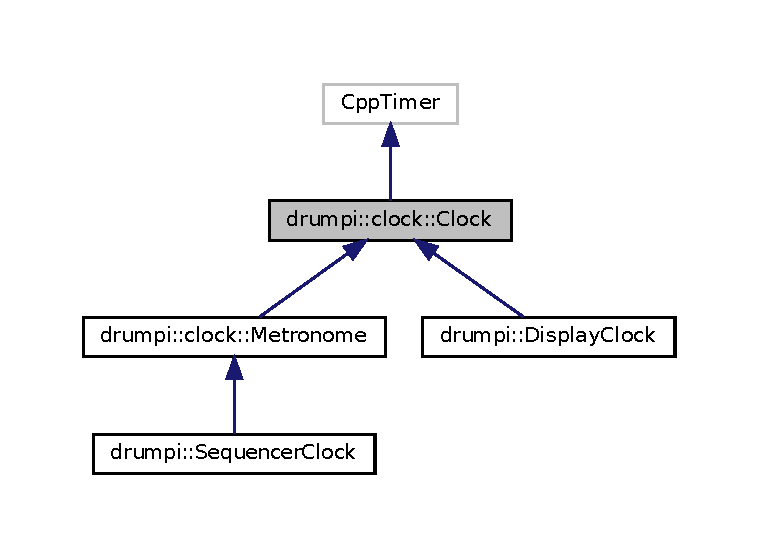
\includegraphics[width=338pt]{classdrumpi_1_1clock_1_1Clock__inherit__graph}
\end{center}
\end{figure}


Collaboration diagram for drumpi\+:\+:clock\+:\+:Clock\+:
\nopagebreak
\begin{figure}[H]
\begin{center}
\leavevmode
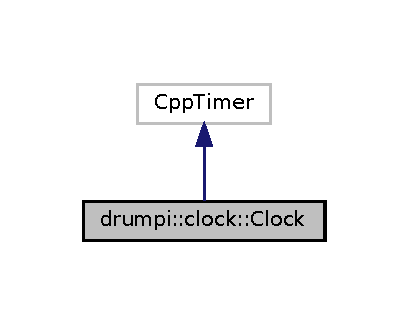
\includegraphics[width=187pt]{classdrumpi_1_1clock_1_1Clock__coll__graph}
\end{center}
\end{figure}
\subsection*{Public Member Functions}
\begin{DoxyCompactItemize}
\item 
\hyperlink{classdrumpi_1_1clock_1_1Clock_adbc370eb6b5f8d01645cf440188160a8}{Clock} ()
\item 
\hyperlink{classdrumpi_1_1clock_1_1Clock_afc976ce68fa85e15cc06f9ed47bddb7c}{$\sim$\+Clock} ()
\item 
void \hyperlink{classdrumpi_1_1clock_1_1Clock_aa9727786f11c753730901fee28cde1ea}{set\+Rate} (int ms)
\item 
int \hyperlink{classdrumpi_1_1clock_1_1Clock_a329b705dad4e8949df7dde09d74b096f}{get\+Rate} ()
\item 
void \hyperlink{classdrumpi_1_1clock_1_1Clock_a8a050959dcff11c85d695989e9099a8c}{start} ()
\item 
void \hyperlink{classdrumpi_1_1clock_1_1Clock_a0b77c3e7f33eb7ae0f018e469d96a250}{stop} ()
\item 
bool \hyperlink{classdrumpi_1_1clock_1_1Clock_a7ea74e7a255c6b426b238982a9e0f349}{is\+Active} ()
\item 
virtual void \hyperlink{classdrumpi_1_1clock_1_1Clock_ade9259c06e6b90bbd92e155a2506d3a1}{tick} ()=0
\end{DoxyCompactItemize}
\subsection*{Protected Attributes}
\begin{DoxyCompactItemize}
\item 
bool \hyperlink{classdrumpi_1_1clock_1_1Clock_a2aa2272f59486b414cedf1345bcf8ea1}{rate\+Change\+Flag}
\end{DoxyCompactItemize}
\subsection*{Private Member Functions}
\begin{DoxyCompactItemize}
\item 
void \hyperlink{classdrumpi_1_1clock_1_1Clock_a2ff18f1fc7761649a9183676b57d543f}{timer\+Event} () override
\end{DoxyCompactItemize}
\subsection*{Private Attributes}
\begin{DoxyCompactItemize}
\item 
int \hyperlink{classdrumpi_1_1clock_1_1Clock_a1ee7e7ba3f9f481c1b9cc9dd72d0e5a9}{rate}
\item 
bool \hyperlink{classdrumpi_1_1clock_1_1Clock_a4ffd1ce8a9bbc4b2fd082f345d81376b}{active}
\end{DoxyCompactItemize}


\subsection{Detailed Description}
Trigger repeated actions. To use, create a class that inherits from this and override the \hyperlink{classdrumpi_1_1clock_1_1Clock_ade9259c06e6b90bbd92e155a2506d3a1}{tick} method to set the functionality. 

\subsection{Constructor \& Destructor Documentation}
\mbox{\Hypertarget{classdrumpi_1_1clock_1_1Clock_adbc370eb6b5f8d01645cf440188160a8}\label{classdrumpi_1_1clock_1_1Clock_adbc370eb6b5f8d01645cf440188160a8}} 
\index{drumpi\+::clock\+::\+Clock@{drumpi\+::clock\+::\+Clock}!Clock@{Clock}}
\index{Clock@{Clock}!drumpi\+::clock\+::\+Clock@{drumpi\+::clock\+::\+Clock}}
\subsubsection{\texorpdfstring{Clock()}{Clock()}}
{\footnotesize\ttfamily Clock\+::\+Clock (\begin{DoxyParamCaption}{ }\end{DoxyParamCaption})}

Constructor. \mbox{\Hypertarget{classdrumpi_1_1clock_1_1Clock_afc976ce68fa85e15cc06f9ed47bddb7c}\label{classdrumpi_1_1clock_1_1Clock_afc976ce68fa85e15cc06f9ed47bddb7c}} 
\index{drumpi\+::clock\+::\+Clock@{drumpi\+::clock\+::\+Clock}!````~Clock@{$\sim$\+Clock}}
\index{````~Clock@{$\sim$\+Clock}!drumpi\+::clock\+::\+Clock@{drumpi\+::clock\+::\+Clock}}
\subsubsection{\texorpdfstring{$\sim$\+Clock()}{~Clock()}}
{\footnotesize\ttfamily Clock\+::$\sim$\+Clock (\begin{DoxyParamCaption}{ }\end{DoxyParamCaption})}

Destructor. Deactivates the clock. 

\subsection{Member Function Documentation}
\mbox{\Hypertarget{classdrumpi_1_1clock_1_1Clock_a329b705dad4e8949df7dde09d74b096f}\label{classdrumpi_1_1clock_1_1Clock_a329b705dad4e8949df7dde09d74b096f}} 
\index{drumpi\+::clock\+::\+Clock@{drumpi\+::clock\+::\+Clock}!get\+Rate@{get\+Rate}}
\index{get\+Rate@{get\+Rate}!drumpi\+::clock\+::\+Clock@{drumpi\+::clock\+::\+Clock}}
\subsubsection{\texorpdfstring{get\+Rate()}{getRate()}}
{\footnotesize\ttfamily int Clock\+::get\+Rate (\begin{DoxyParamCaption}{ }\end{DoxyParamCaption})}

Returns the clock rate in ms. \begin{DoxyReturn}{Returns}
clock rate in ms. 
\end{DoxyReturn}
\mbox{\Hypertarget{classdrumpi_1_1clock_1_1Clock_a7ea74e7a255c6b426b238982a9e0f349}\label{classdrumpi_1_1clock_1_1Clock_a7ea74e7a255c6b426b238982a9e0f349}} 
\index{drumpi\+::clock\+::\+Clock@{drumpi\+::clock\+::\+Clock}!is\+Active@{is\+Active}}
\index{is\+Active@{is\+Active}!drumpi\+::clock\+::\+Clock@{drumpi\+::clock\+::\+Clock}}
\subsubsection{\texorpdfstring{is\+Active()}{isActive()}}
{\footnotesize\ttfamily bool Clock\+::is\+Active (\begin{DoxyParamCaption}{ }\end{DoxyParamCaption})}

Checks if the \hyperlink{classdrumpi_1_1clock_1_1Clock}{Clock} is active. \begin{DoxyReturn}{Returns}
{\ttfamily true} if active. 
\end{DoxyReturn}
\mbox{\Hypertarget{classdrumpi_1_1clock_1_1Clock_aa9727786f11c753730901fee28cde1ea}\label{classdrumpi_1_1clock_1_1Clock_aa9727786f11c753730901fee28cde1ea}} 
\index{drumpi\+::clock\+::\+Clock@{drumpi\+::clock\+::\+Clock}!set\+Rate@{set\+Rate}}
\index{set\+Rate@{set\+Rate}!drumpi\+::clock\+::\+Clock@{drumpi\+::clock\+::\+Clock}}
\subsubsection{\texorpdfstring{set\+Rate()}{setRate()}}
{\footnotesize\ttfamily void Clock\+::set\+Rate (\begin{DoxyParamCaption}\item[{int}]{ms }\end{DoxyParamCaption})}

Set the clock rate. The change takes effect on the next \hyperlink{classdrumpi_1_1clock_1_1Clock_ade9259c06e6b90bbd92e155a2506d3a1}{tick}, or can be forced by calling \hyperlink{classdrumpi_1_1clock_1_1Clock_a0b77c3e7f33eb7ae0f018e469d96a250}{stop} and then \hyperlink{classdrumpi_1_1clock_1_1Clock_a8a050959dcff11c85d695989e9099a8c}{start}. 
\begin{DoxyParams}{Parameters}
{\em ms} & desired clocking rate in ms. \\
\hline
\end{DoxyParams}
\mbox{\Hypertarget{classdrumpi_1_1clock_1_1Clock_a8a050959dcff11c85d695989e9099a8c}\label{classdrumpi_1_1clock_1_1Clock_a8a050959dcff11c85d695989e9099a8c}} 
\index{drumpi\+::clock\+::\+Clock@{drumpi\+::clock\+::\+Clock}!start@{start}}
\index{start@{start}!drumpi\+::clock\+::\+Clock@{drumpi\+::clock\+::\+Clock}}
\subsubsection{\texorpdfstring{start()}{start()}}
{\footnotesize\ttfamily void Clock\+::start (\begin{DoxyParamCaption}{ }\end{DoxyParamCaption})}

Start the clock. Default period is 1 second, change with \hyperlink{classdrumpi_1_1clock_1_1Clock_aa9727786f11c753730901fee28cde1ea}{set\+Rate}. \mbox{\Hypertarget{classdrumpi_1_1clock_1_1Clock_a0b77c3e7f33eb7ae0f018e469d96a250}\label{classdrumpi_1_1clock_1_1Clock_a0b77c3e7f33eb7ae0f018e469d96a250}} 
\index{drumpi\+::clock\+::\+Clock@{drumpi\+::clock\+::\+Clock}!stop@{stop}}
\index{stop@{stop}!drumpi\+::clock\+::\+Clock@{drumpi\+::clock\+::\+Clock}}
\subsubsection{\texorpdfstring{stop()}{stop()}}
{\footnotesize\ttfamily void Clock\+::stop (\begin{DoxyParamCaption}{ }\end{DoxyParamCaption})}

Stop the clock. \mbox{\Hypertarget{classdrumpi_1_1clock_1_1Clock_ade9259c06e6b90bbd92e155a2506d3a1}\label{classdrumpi_1_1clock_1_1Clock_ade9259c06e6b90bbd92e155a2506d3a1}} 
\index{drumpi\+::clock\+::\+Clock@{drumpi\+::clock\+::\+Clock}!tick@{tick}}
\index{tick@{tick}!drumpi\+::clock\+::\+Clock@{drumpi\+::clock\+::\+Clock}}
\subsubsection{\texorpdfstring{tick()}{tick()}}
{\footnotesize\ttfamily virtual void drumpi\+::clock\+::\+Clock\+::tick (\begin{DoxyParamCaption}{ }\end{DoxyParamCaption})\hspace{0.3cm}{\ttfamily [pure virtual]}}

Callback method run on each clock pulse. Override to add functionality. 

Implemented in \hyperlink{classdrumpi_1_1SequencerClock_ac75142ddc2ee0dcd3c52d13e44b0d85f}{drumpi\+::\+Sequencer\+Clock}, and \hyperlink{classdrumpi_1_1DisplayClock_ae44b216f4788398ab3d67da7141fa88f}{drumpi\+::\+Display\+Clock}.

\mbox{\Hypertarget{classdrumpi_1_1clock_1_1Clock_a2ff18f1fc7761649a9183676b57d543f}\label{classdrumpi_1_1clock_1_1Clock_a2ff18f1fc7761649a9183676b57d543f}} 
\index{drumpi\+::clock\+::\+Clock@{drumpi\+::clock\+::\+Clock}!timer\+Event@{timer\+Event}}
\index{timer\+Event@{timer\+Event}!drumpi\+::clock\+::\+Clock@{drumpi\+::clock\+::\+Clock}}
\subsubsection{\texorpdfstring{timer\+Event()}{timerEvent()}}
{\footnotesize\ttfamily void Clock\+::timer\+Event (\begin{DoxyParamCaption}{ }\end{DoxyParamCaption})\hspace{0.3cm}{\ttfamily [override]}, {\ttfamily [private]}}

Override event method to call \hyperlink{classdrumpi_1_1clock_1_1Clock_ade9259c06e6b90bbd92e155a2506d3a1}{tick()}. 

\subsection{Member Data Documentation}
\mbox{\Hypertarget{classdrumpi_1_1clock_1_1Clock_a4ffd1ce8a9bbc4b2fd082f345d81376b}\label{classdrumpi_1_1clock_1_1Clock_a4ffd1ce8a9bbc4b2fd082f345d81376b}} 
\index{drumpi\+::clock\+::\+Clock@{drumpi\+::clock\+::\+Clock}!active@{active}}
\index{active@{active}!drumpi\+::clock\+::\+Clock@{drumpi\+::clock\+::\+Clock}}
\subsubsection{\texorpdfstring{active}{active}}
{\footnotesize\ttfamily bool drumpi\+::clock\+::\+Clock\+::active\hspace{0.3cm}{\ttfamily [private]}}

Active flag. \mbox{\Hypertarget{classdrumpi_1_1clock_1_1Clock_a1ee7e7ba3f9f481c1b9cc9dd72d0e5a9}\label{classdrumpi_1_1clock_1_1Clock_a1ee7e7ba3f9f481c1b9cc9dd72d0e5a9}} 
\index{drumpi\+::clock\+::\+Clock@{drumpi\+::clock\+::\+Clock}!rate@{rate}}
\index{rate@{rate}!drumpi\+::clock\+::\+Clock@{drumpi\+::clock\+::\+Clock}}
\subsubsection{\texorpdfstring{rate}{rate}}
{\footnotesize\ttfamily int drumpi\+::clock\+::\+Clock\+::rate\hspace{0.3cm}{\ttfamily [private]}}

\hyperlink{classdrumpi_1_1clock_1_1Clock}{Clock} rate in ms. \mbox{\Hypertarget{classdrumpi_1_1clock_1_1Clock_a2aa2272f59486b414cedf1345bcf8ea1}\label{classdrumpi_1_1clock_1_1Clock_a2aa2272f59486b414cedf1345bcf8ea1}} 
\index{drumpi\+::clock\+::\+Clock@{drumpi\+::clock\+::\+Clock}!rate\+Change\+Flag@{rate\+Change\+Flag}}
\index{rate\+Change\+Flag@{rate\+Change\+Flag}!drumpi\+::clock\+::\+Clock@{drumpi\+::clock\+::\+Clock}}
\subsubsection{\texorpdfstring{rate\+Change\+Flag}{rateChangeFlag}}
{\footnotesize\ttfamily bool drumpi\+::clock\+::\+Clock\+::rate\+Change\+Flag\hspace{0.3cm}{\ttfamily [protected]}}

Flag for the clocking rate being changed. 

The documentation for this class was generated from the following files\+:\begin{DoxyCompactItemize}
\item 
src/clock.\+hpp\item 
src/clock.\+cpp\end{DoxyCompactItemize}

\hypertarget{classdrumpi_1_1Display}{}\section{drumpi\+:\+:Display Class Reference}
\label{classdrumpi_1_1Display}\index{drumpi\+::\+Display@{drumpi\+::\+Display}}


{\ttfamily \#include $<$display.\+hpp$>$}



Inheritance diagram for drumpi\+:\+:Display\+:
\nopagebreak
\begin{figure}[H]
\begin{center}
\leavevmode
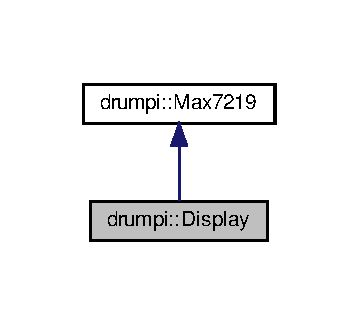
\includegraphics[width=172pt]{classdrumpi_1_1Display__inherit__graph}
\end{center}
\end{figure}


Collaboration diagram for drumpi\+:\+:Display\+:
\nopagebreak
\begin{figure}[H]
\begin{center}
\leavevmode
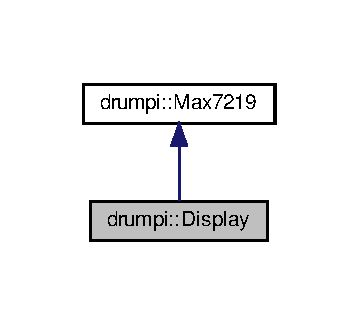
\includegraphics[width=172pt]{classdrumpi_1_1Display__coll__graph}
\end{center}
\end{figure}
\subsection*{Public Member Functions}
\begin{DoxyCompactItemize}
\item 
\mbox{\Hypertarget{classdrumpi_1_1Display_ac2607a6bb236c55547a4223d40d85d1f}\label{classdrumpi_1_1Display_ac2607a6bb236c55547a4223d40d85d1f}} 
\hyperlink{classdrumpi_1_1Display_ac2607a6bb236c55547a4223d40d85d1f}{$\sim$\+Display} ()
\begin{DoxyCompactList}\small\item\em Constructor. \end{DoxyCompactList}\item 
void \hyperlink{classdrumpi_1_1Display_a736439f0512941aed6a870343a6dfcb4}{set\+Val} (unsigned int value, bool redraw)
\begin{DoxyCompactList}\small\item\em Destructor. \end{DoxyCompactList}\item 
void \hyperlink{classdrumpi_1_1Display_a7ddc806af584e6cde78b68400aac9a32}{set\+Drum\+Volume} (unsigned int value, \hyperlink{namespacedrumpi_a3897274035c1b939a604438abe648b1b}{drum\+I\+D\+\_\+t} current\+Drum, bool redraw)
\item 
void \hyperlink{classdrumpi_1_1Display_a2da5a80f0fe89c46142fb612e89a3bbc}{set\+Keymapping} (std\+::vector$<$ unsigned int $>$ \+\_\+key\+Mapping)
\item 
void \hyperlink{classdrumpi_1_1Display_a7b1a1df8eb13768b89c5b48eb2b319eb}{set\+Playback\+Seq} (std\+::vector$<$ bool $>$ active\+Drums, unsigned int step\+Num, bool redraw)
\item 
void \hyperlink{classdrumpi_1_1Display_ae253a08f20fdd1256658c81c64164dbd}{set\+Stop\+Seq} (std\+::vector$<$ bool $>$ active\+Drums, unsigned int page, \hyperlink{namespacedrumpi_a3897274035c1b939a604438abe648b1b}{drum\+I\+D\+\_\+t} current\+Drum, bool redraw)
\item 
void \hyperlink{classdrumpi_1_1Display_a695bf2d6c688b87ad88bc3fbd8fa1fff}{set\+Performance} (std\+::vector$<$ \hyperlink{namespacedrumpi_a3897274035c1b939a604438abe648b1b}{drum\+I\+D\+\_\+t} $>$ active\+Drums, float level, bool redraw)
\item 
int \hyperlink{classdrumpi_1_1Display_a98f1e8a6fe644f75dc086cf23c5687c6}{get\+Keymapping} (int index)
\end{DoxyCompactItemize}
\subsection*{Private Member Functions}
\begin{DoxyCompactItemize}
\item 
void \hyperlink{classdrumpi_1_1Display_acd75af285265d26173f4481a92eb5d8c}{set\+Three\+Digit} (unsigned int value)
\item 
void \hyperlink{classdrumpi_1_1Display_a6430f2a097b1c2d3cd71e7d4ee9e375c}{set\+Two\+Digit} (unsigned int value)
\item 
void \hyperlink{classdrumpi_1_1Display_ade135706a915e866e06ec8c30202ee79}{set\+One\+Digit} (unsigned int value)
\item 
void \hyperlink{classdrumpi_1_1Display_ad80799724d362dcbb260d368bfdc18c3}{set\+Active\+Drums} (std\+::vector$<$ bool $>$ active\+Drums, unsigned int page)
\item 
void \hyperlink{classdrumpi_1_1Display_aed0dfcb7bbf5209a9a1501e2d63fe947}{add\+Level} (float level)
\item 
void \hyperlink{classdrumpi_1_1Display_a8ff778f88ca14acb0232b0afec54b972}{add\+Page} (unsigned int page)
\end{DoxyCompactItemize}
\subsection*{Private Attributes}
\begin{DoxyCompactItemize}
\item 
const std\+::vector$<$ unsigned char $>$ \hyperlink{classdrumpi_1_1Display_a6a545666c68e6fc74c386d47e1b86635}{dec\+Hex\+Vals}
\item 
const unsigned char \hyperlink{classdrumpi_1_1Display_a262abe3f60fd889ec627bf3e08f1468e}{dp\+Addr} = 0x80
\item 
const unsigned char \hyperlink{classdrumpi_1_1Display_a6edbae4cb83ea5fd2e37fb0549abec58}{upper\+Sq\+Addr} = 0x63
\item 
const unsigned char \hyperlink{classdrumpi_1_1Display_a071f2149fd9687d8b3c33fb92fe08fb1}{bottom\+Addr} = 0x8
\item 
std\+::vector$<$ unsigned int $>$ \hyperlink{classdrumpi_1_1Display_ae168cc9f5c514995b51c483b81f6be2b}{key\+Mapping}
\end{DoxyCompactItemize}


\subsection{Detailed Description}
High level Drum\+Pi display driver 

\subsection{Member Function Documentation}
\mbox{\Hypertarget{classdrumpi_1_1Display_aed0dfcb7bbf5209a9a1501e2d63fe947}\label{classdrumpi_1_1Display_aed0dfcb7bbf5209a9a1501e2d63fe947}} 
\index{drumpi\+::\+Display@{drumpi\+::\+Display}!add\+Level@{add\+Level}}
\index{add\+Level@{add\+Level}!drumpi\+::\+Display@{drumpi\+::\+Display}}
\subsubsection{\texorpdfstring{add\+Level()}{addLevel()}}
{\footnotesize\ttfamily void Display\+::add\+Level (\begin{DoxyParamCaption}\item[{float}]{level }\end{DoxyParamCaption})\hspace{0.3cm}{\ttfamily [private]}}

Adds to values in \hyperlink{classdrumpi_1_1Max7219_ab26f32728dd82c00e39b6212436f291e}{digit\+Buffer} to show an audio level.

Not implemented in V1.\+0. 
\begin{DoxyParams}{Parameters}
{\em level} & Audio level to display. \\
\hline
\end{DoxyParams}
\mbox{\Hypertarget{classdrumpi_1_1Display_a8ff778f88ca14acb0232b0afec54b972}\label{classdrumpi_1_1Display_a8ff778f88ca14acb0232b0afec54b972}} 
\index{drumpi\+::\+Display@{drumpi\+::\+Display}!add\+Page@{add\+Page}}
\index{add\+Page@{add\+Page}!drumpi\+::\+Display@{drumpi\+::\+Display}}
\subsubsection{\texorpdfstring{add\+Page()}{addPage()}}
{\footnotesize\ttfamily void Display\+::add\+Page (\begin{DoxyParamCaption}\item[{unsigned int}]{page }\end{DoxyParamCaption})\hspace{0.3cm}{\ttfamily [private]}}

Adds to values in \hyperlink{classdrumpi_1_1Max7219_ab26f32728dd82c00e39b6212436f291e}{digit\+Buffer} to show the current page.


\begin{DoxyParams}{Parameters}
{\em page} & Page to display. \\
\hline
\end{DoxyParams}
\mbox{\Hypertarget{classdrumpi_1_1Display_a98f1e8a6fe644f75dc086cf23c5687c6}\label{classdrumpi_1_1Display_a98f1e8a6fe644f75dc086cf23c5687c6}} 
\index{drumpi\+::\+Display@{drumpi\+::\+Display}!get\+Keymapping@{get\+Keymapping}}
\index{get\+Keymapping@{get\+Keymapping}!drumpi\+::\+Display@{drumpi\+::\+Display}}
\subsubsection{\texorpdfstring{get\+Keymapping()}{getKeymapping()}}
{\footnotesize\ttfamily int Display\+::get\+Keymapping (\begin{DoxyParamCaption}\item[{int}]{index }\end{DoxyParamCaption})}

Returns a key mapping. 
\begin{DoxyParams}{Parameters}
{\em index} & Drum\+Id to query. \\
\hline
\end{DoxyParams}
\mbox{\Hypertarget{classdrumpi_1_1Display_ad80799724d362dcbb260d368bfdc18c3}\label{classdrumpi_1_1Display_ad80799724d362dcbb260d368bfdc18c3}} 
\index{drumpi\+::\+Display@{drumpi\+::\+Display}!set\+Active\+Drums@{set\+Active\+Drums}}
\index{set\+Active\+Drums@{set\+Active\+Drums}!drumpi\+::\+Display@{drumpi\+::\+Display}}
\subsubsection{\texorpdfstring{set\+Active\+Drums()}{setActiveDrums()}}
{\footnotesize\ttfamily void Display\+::set\+Active\+Drums (\begin{DoxyParamCaption}\item[{std\+::vector$<$ bool $>$}]{active\+Drums,  }\item[{unsigned int}]{page }\end{DoxyParamCaption})\hspace{0.3cm}{\ttfamily [private]}}

Sets values in the \hyperlink{classdrumpi_1_1Max7219_ab26f32728dd82c00e39b6212436f291e}{digit\+Buffer} to show active drums for a given sequence and page.


\begin{DoxyParams}{Parameters}
{\em active\+Drums} & Vector of bools representing sequence. \\
\hline
{\em page} & 8 digit page to display. \\
\hline
\end{DoxyParams}
\mbox{\Hypertarget{classdrumpi_1_1Display_a7ddc806af584e6cde78b68400aac9a32}\label{classdrumpi_1_1Display_a7ddc806af584e6cde78b68400aac9a32}} 
\index{drumpi\+::\+Display@{drumpi\+::\+Display}!set\+Drum\+Volume@{set\+Drum\+Volume}}
\index{set\+Drum\+Volume@{set\+Drum\+Volume}!drumpi\+::\+Display@{drumpi\+::\+Display}}
\subsubsection{\texorpdfstring{set\+Drum\+Volume()}{setDrumVolume()}}
{\footnotesize\ttfamily void Display\+::set\+Drum\+Volume (\begin{DoxyParamCaption}\item[{unsigned int}]{value,  }\item[{\hyperlink{namespacedrumpi_a3897274035c1b939a604438abe648b1b}{drum\+I\+D\+\_\+t}}]{current\+Drum,  }\item[{bool}]{redraw }\end{DoxyParamCaption})}

Sets values in \hyperlink{classdrumpi_1_1Max7219_ab26f32728dd82c00e39b6212436f291e}{digit\+Buffer} to display a drum volume and current drum.


\begin{DoxyParams}{Parameters}
{\em value} & Numerical value to display. \\
\hline
{\em current\+Drum} & Current drum to display. \\
\hline
{\em redraw} & If true, updates display. \\
\hline
\end{DoxyParams}
\mbox{\Hypertarget{classdrumpi_1_1Display_a2da5a80f0fe89c46142fb612e89a3bbc}\label{classdrumpi_1_1Display_a2da5a80f0fe89c46142fb612e89a3bbc}} 
\index{drumpi\+::\+Display@{drumpi\+::\+Display}!set\+Keymapping@{set\+Keymapping}}
\index{set\+Keymapping@{set\+Keymapping}!drumpi\+::\+Display@{drumpi\+::\+Display}}
\subsubsection{\texorpdfstring{set\+Keymapping()}{setKeymapping()}}
{\footnotesize\ttfamily void Display\+::set\+Keymapping (\begin{DoxyParamCaption}\item[{std\+::vector$<$ unsigned int $>$}]{\+\_\+key\+Mapping }\end{DoxyParamCaption})}

Sets the mapping of drums to keys. Ensuring that the correct digits are displayed.

Currently unused in v1.\+0.


\begin{DoxyParams}{Parameters}
{\em \+\_\+key\+Mapping} & The given mapping to set. \\
\hline
\end{DoxyParams}
\mbox{\Hypertarget{classdrumpi_1_1Display_ade135706a915e866e06ec8c30202ee79}\label{classdrumpi_1_1Display_ade135706a915e866e06ec8c30202ee79}} 
\index{drumpi\+::\+Display@{drumpi\+::\+Display}!set\+One\+Digit@{set\+One\+Digit}}
\index{set\+One\+Digit@{set\+One\+Digit}!drumpi\+::\+Display@{drumpi\+::\+Display}}
\subsubsection{\texorpdfstring{set\+One\+Digit()}{setOneDigit()}}
{\footnotesize\ttfamily void Display\+::set\+One\+Digit (\begin{DoxyParamCaption}\item[{unsigned int}]{value }\end{DoxyParamCaption})\hspace{0.3cm}{\ttfamily [private]}}

Sets a 1 digit decimal value. 
\begin{DoxyParams}{Parameters}
{\em value} & 1 digit value to set. \\
\hline
\end{DoxyParams}
\mbox{\Hypertarget{classdrumpi_1_1Display_a695bf2d6c688b87ad88bc3fbd8fa1fff}\label{classdrumpi_1_1Display_a695bf2d6c688b87ad88bc3fbd8fa1fff}} 
\index{drumpi\+::\+Display@{drumpi\+::\+Display}!set\+Performance@{set\+Performance}}
\index{set\+Performance@{set\+Performance}!drumpi\+::\+Display@{drumpi\+::\+Display}}
\subsubsection{\texorpdfstring{set\+Performance()}{setPerformance()}}
{\footnotesize\ttfamily void Display\+::set\+Performance (\begin{DoxyParamCaption}\item[{std\+::vector$<$ \hyperlink{namespacedrumpi_a3897274035c1b939a604438abe648b1b}{drum\+I\+D\+\_\+t} $>$}]{active\+Drums,  }\item[{float}]{level,  }\item[{bool}]{redraw }\end{DoxyParamCaption})}

Sets values in \hyperlink{classdrumpi_1_1Max7219_ab26f32728dd82c00e39b6212436f291e}{digit\+Buffer} to show performance display.


\begin{DoxyParams}{Parameters}
{\em active\+Drums} & Vector containing \hyperlink{namespacedrumpi_a3897274035c1b939a604438abe648b1b}{drum\+I\+D\+\_\+t} of all current drums. \\
\hline
{\em level} & Audio level. \\
\hline
{\em redraw} & If true, updates display. \\
\hline
\end{DoxyParams}
\mbox{\Hypertarget{classdrumpi_1_1Display_a7b1a1df8eb13768b89c5b48eb2b319eb}\label{classdrumpi_1_1Display_a7b1a1df8eb13768b89c5b48eb2b319eb}} 
\index{drumpi\+::\+Display@{drumpi\+::\+Display}!set\+Playback\+Seq@{set\+Playback\+Seq}}
\index{set\+Playback\+Seq@{set\+Playback\+Seq}!drumpi\+::\+Display@{drumpi\+::\+Display}}
\subsubsection{\texorpdfstring{set\+Playback\+Seq()}{setPlaybackSeq()}}
{\footnotesize\ttfamily void Display\+::set\+Playback\+Seq (\begin{DoxyParamCaption}\item[{std\+::vector$<$ bool $>$}]{active\+Drums,  }\item[{unsigned int}]{step\+Num,  }\item[{bool}]{redraw }\end{DoxyParamCaption})}

Sets values in \hyperlink{classdrumpi_1_1Max7219_ab26f32728dd82c00e39b6212436f291e}{digit\+Buffer} to show sequence in playback mode.


\begin{DoxyParams}{Parameters}
{\em active\+Drums} & Vector of bools representing sequence. \\
\hline
{\em step\+Num} & Current step in sequence. \\
\hline
{\em redraw} & If true, updates display. \\
\hline
\end{DoxyParams}
\mbox{\Hypertarget{classdrumpi_1_1Display_ae253a08f20fdd1256658c81c64164dbd}\label{classdrumpi_1_1Display_ae253a08f20fdd1256658c81c64164dbd}} 
\index{drumpi\+::\+Display@{drumpi\+::\+Display}!set\+Stop\+Seq@{set\+Stop\+Seq}}
\index{set\+Stop\+Seq@{set\+Stop\+Seq}!drumpi\+::\+Display@{drumpi\+::\+Display}}
\subsubsection{\texorpdfstring{set\+Stop\+Seq()}{setStopSeq()}}
{\footnotesize\ttfamily void Display\+::set\+Stop\+Seq (\begin{DoxyParamCaption}\item[{std\+::vector$<$ bool $>$}]{active\+Drums,  }\item[{unsigned int}]{page,  }\item[{\hyperlink{namespacedrumpi_a3897274035c1b939a604438abe648b1b}{drum\+I\+D\+\_\+t}}]{current\+Drum,  }\item[{bool}]{redraw }\end{DoxyParamCaption})}

Sets values in \hyperlink{classdrumpi_1_1Max7219_ab26f32728dd82c00e39b6212436f291e}{digit\+Buffer} to show sequence in stop mode.


\begin{DoxyParams}{Parameters}
{\em active\+Drums} & Vector of bools representing sequence. \\
\hline
{\em page} & Current page to display. \\
\hline
{\em current\+Drum} & Active drum for editing. \\
\hline
{\em redraw} & If true, updates display. \\
\hline
\end{DoxyParams}
\mbox{\Hypertarget{classdrumpi_1_1Display_acd75af285265d26173f4481a92eb5d8c}\label{classdrumpi_1_1Display_acd75af285265d26173f4481a92eb5d8c}} 
\index{drumpi\+::\+Display@{drumpi\+::\+Display}!set\+Three\+Digit@{set\+Three\+Digit}}
\index{set\+Three\+Digit@{set\+Three\+Digit}!drumpi\+::\+Display@{drumpi\+::\+Display}}
\subsubsection{\texorpdfstring{set\+Three\+Digit()}{setThreeDigit()}}
{\footnotesize\ttfamily void Display\+::set\+Three\+Digit (\begin{DoxyParamCaption}\item[{unsigned int}]{value }\end{DoxyParamCaption})\hspace{0.3cm}{\ttfamily [private]}}

Sets a 3 digit decimal value. 
\begin{DoxyParams}{Parameters}
{\em value} & 3 digit value to set. \\
\hline
\end{DoxyParams}
\mbox{\Hypertarget{classdrumpi_1_1Display_a6430f2a097b1c2d3cd71e7d4ee9e375c}\label{classdrumpi_1_1Display_a6430f2a097b1c2d3cd71e7d4ee9e375c}} 
\index{drumpi\+::\+Display@{drumpi\+::\+Display}!set\+Two\+Digit@{set\+Two\+Digit}}
\index{set\+Two\+Digit@{set\+Two\+Digit}!drumpi\+::\+Display@{drumpi\+::\+Display}}
\subsubsection{\texorpdfstring{set\+Two\+Digit()}{setTwoDigit()}}
{\footnotesize\ttfamily void Display\+::set\+Two\+Digit (\begin{DoxyParamCaption}\item[{unsigned int}]{value }\end{DoxyParamCaption})\hspace{0.3cm}{\ttfamily [private]}}

Sets a 2 digit decimal value. 
\begin{DoxyParams}{Parameters}
{\em value} & 2 digit value to set. \\
\hline
\end{DoxyParams}
\mbox{\Hypertarget{classdrumpi_1_1Display_a736439f0512941aed6a870343a6dfcb4}\label{classdrumpi_1_1Display_a736439f0512941aed6a870343a6dfcb4}} 
\index{drumpi\+::\+Display@{drumpi\+::\+Display}!set\+Val@{set\+Val}}
\index{set\+Val@{set\+Val}!drumpi\+::\+Display@{drumpi\+::\+Display}}
\subsubsection{\texorpdfstring{set\+Val()}{setVal()}}
{\footnotesize\ttfamily void Display\+::set\+Val (\begin{DoxyParamCaption}\item[{unsigned int}]{value,  }\item[{bool}]{redraw }\end{DoxyParamCaption})}



Destructor. 

Sets values in \hyperlink{classdrumpi_1_1Max7219_ab26f32728dd82c00e39b6212436f291e}{digit\+Buffer} to display a number up to 999.


\begin{DoxyParams}{Parameters}
{\em value} & Numerical value to display. \\
\hline
{\em redraw} & If true, updates display. \\
\hline
\end{DoxyParams}


\subsection{Member Data Documentation}
\mbox{\Hypertarget{classdrumpi_1_1Display_a071f2149fd9687d8b3c33fb92fe08fb1}\label{classdrumpi_1_1Display_a071f2149fd9687d8b3c33fb92fe08fb1}} 
\index{drumpi\+::\+Display@{drumpi\+::\+Display}!bottom\+Addr@{bottom\+Addr}}
\index{bottom\+Addr@{bottom\+Addr}!drumpi\+::\+Display@{drumpi\+::\+Display}}
\subsubsection{\texorpdfstring{bottom\+Addr}{bottomAddr}}
{\footnotesize\ttfamily const unsigned char drumpi\+::\+Display\+::bottom\+Addr = 0x8\hspace{0.3cm}{\ttfamily [private]}}

Hex address for bottom underscore segment. \mbox{\Hypertarget{classdrumpi_1_1Display_a6a545666c68e6fc74c386d47e1b86635}\label{classdrumpi_1_1Display_a6a545666c68e6fc74c386d47e1b86635}} 
\index{drumpi\+::\+Display@{drumpi\+::\+Display}!dec\+Hex\+Vals@{dec\+Hex\+Vals}}
\index{dec\+Hex\+Vals@{dec\+Hex\+Vals}!drumpi\+::\+Display@{drumpi\+::\+Display}}
\subsubsection{\texorpdfstring{dec\+Hex\+Vals}{decHexVals}}
{\footnotesize\ttfamily const std\+::vector$<$unsigned char$>$ drumpi\+::\+Display\+::dec\+Hex\+Vals\hspace{0.3cm}{\ttfamily [private]}}

{\bfseries Initial value\+:}
\begin{DoxyCode}
= \{
            0x7E, 
            0x30, 
            0x6D, 
            0x79, 
            0x33, 
            0x5B, 
            0x5F, 
            0x70, 
            0x7F, 
            0x7B, 
        \}
\end{DoxyCode}
Vector to contain corresponding hex values for decimal digit representation.

Prevents the need to toggle Code B decode for every numerical display. \mbox{\Hypertarget{classdrumpi_1_1Display_a262abe3f60fd889ec627bf3e08f1468e}\label{classdrumpi_1_1Display_a262abe3f60fd889ec627bf3e08f1468e}} 
\index{drumpi\+::\+Display@{drumpi\+::\+Display}!dp\+Addr@{dp\+Addr}}
\index{dp\+Addr@{dp\+Addr}!drumpi\+::\+Display@{drumpi\+::\+Display}}
\subsubsection{\texorpdfstring{dp\+Addr}{dpAddr}}
{\footnotesize\ttfamily const unsigned char drumpi\+::\+Display\+::dp\+Addr = 0x80\hspace{0.3cm}{\ttfamily [private]}}

Hex address for decimal place. \mbox{\Hypertarget{classdrumpi_1_1Display_ae168cc9f5c514995b51c483b81f6be2b}\label{classdrumpi_1_1Display_ae168cc9f5c514995b51c483b81f6be2b}} 
\index{drumpi\+::\+Display@{drumpi\+::\+Display}!key\+Mapping@{key\+Mapping}}
\index{key\+Mapping@{key\+Mapping}!drumpi\+::\+Display@{drumpi\+::\+Display}}
\subsubsection{\texorpdfstring{key\+Mapping}{keyMapping}}
{\footnotesize\ttfamily std\+::vector$<$unsigned int$>$ drumpi\+::\+Display\+::key\+Mapping\hspace{0.3cm}{\ttfamily [private]}}

{\bfseries Initial value\+:}
\begin{DoxyCode}
= \{
            0,  
            1,  
            2,  
            3,  
            4,  
            5,  
            6,  
            7,  
        \}
\end{DoxyCode}
Vector to contain key mappings.

key\+Mapping\mbox{[}drum\+ID\mbox{]} = key/digit. \mbox{\Hypertarget{classdrumpi_1_1Display_a6edbae4cb83ea5fd2e37fb0549abec58}\label{classdrumpi_1_1Display_a6edbae4cb83ea5fd2e37fb0549abec58}} 
\index{drumpi\+::\+Display@{drumpi\+::\+Display}!upper\+Sq\+Addr@{upper\+Sq\+Addr}}
\index{upper\+Sq\+Addr@{upper\+Sq\+Addr}!drumpi\+::\+Display@{drumpi\+::\+Display}}
\subsubsection{\texorpdfstring{upper\+Sq\+Addr}{upperSqAddr}}
{\footnotesize\ttfamily const unsigned char drumpi\+::\+Display\+::upper\+Sq\+Addr = 0x63\hspace{0.3cm}{\ttfamily [private]}}

Hex address for upper square. 

The documentation for this class was generated from the following files\+:\begin{DoxyCompactItemize}
\item 
src/display.\+hpp\item 
src/display.\+cpp\end{DoxyCompactItemize}

\hypertarget{classdrumpi_1_1DisplayClock}{}\section{drumpi\+:\+:Display\+Clock Class Reference}
\label{classdrumpi_1_1DisplayClock}\index{drumpi\+::\+Display\+Clock@{drumpi\+::\+Display\+Clock}}


{\ttfamily \#include $<$application.\+hpp$>$}



Inheritance diagram for drumpi\+:\+:Display\+Clock\+:
\nopagebreak
\begin{figure}[H]
\begin{center}
\leavevmode
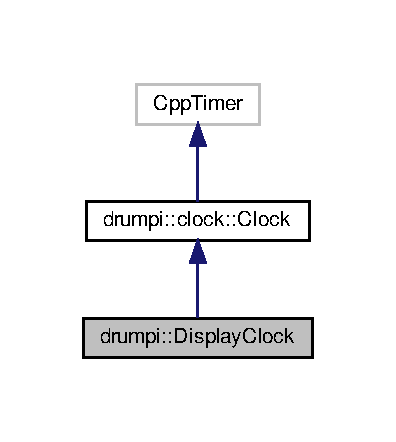
\includegraphics[width=190pt]{classdrumpi_1_1DisplayClock__inherit__graph}
\end{center}
\end{figure}


Collaboration diagram for drumpi\+:\+:Display\+Clock\+:
\nopagebreak
\begin{figure}[H]
\begin{center}
\leavevmode
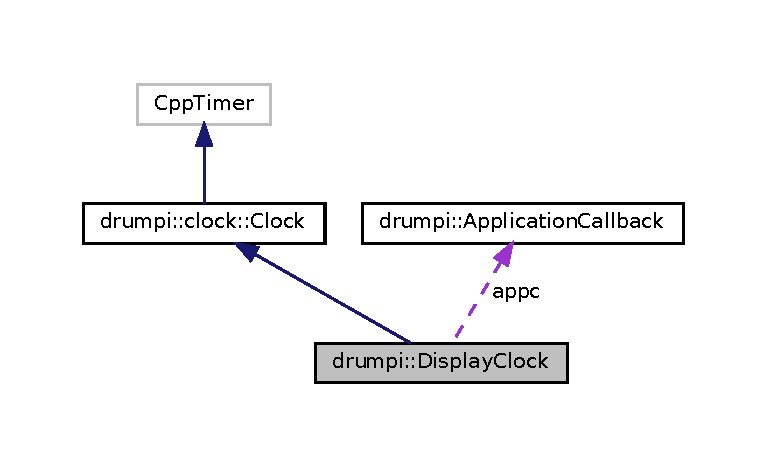
\includegraphics[width=344pt]{classdrumpi_1_1DisplayClock__coll__graph}
\end{center}
\end{figure}
\subsection*{Public Member Functions}
\begin{DoxyCompactItemize}
\item 
\hyperlink{classdrumpi_1_1DisplayClock_a16708f6b73c6253107d1db24cf7396dc}{Display\+Clock} (\hyperlink{classdrumpi_1_1ApplicationCallback}{Application\+Callback} $\ast$a)
\item 
void \hyperlink{classdrumpi_1_1DisplayClock_ae44b216f4788398ab3d67da7141fa88f}{tick} () override
\end{DoxyCompactItemize}
\subsection*{Private Attributes}
\begin{DoxyCompactItemize}
\item 
\hyperlink{classdrumpi_1_1ApplicationCallback}{Application\+Callback} $\ast$ \hyperlink{classdrumpi_1_1DisplayClock_a85d58654905b372a83fa258ab2d5a1b0}{appc} = nullptr
\end{DoxyCompactItemize}
\subsection*{Additional Inherited Members}


\subsection{Detailed Description}
\hyperlink{classdrumpi_1_1clock_1_1Metronome}{clock\+::\+Metronome} derived class to clock a \hyperlink{classdrumpi_1_1Display}{Display}. 

\subsection{Constructor \& Destructor Documentation}
\mbox{\Hypertarget{classdrumpi_1_1DisplayClock_a16708f6b73c6253107d1db24cf7396dc}\label{classdrumpi_1_1DisplayClock_a16708f6b73c6253107d1db24cf7396dc}} 
\index{drumpi\+::\+Display\+Clock@{drumpi\+::\+Display\+Clock}!Display\+Clock@{Display\+Clock}}
\index{Display\+Clock@{Display\+Clock}!drumpi\+::\+Display\+Clock@{drumpi\+::\+Display\+Clock}}
\subsubsection{\texorpdfstring{Display\+Clock()}{DisplayClock()}}
{\footnotesize\ttfamily Display\+Clock\+::\+Display\+Clock (\begin{DoxyParamCaption}\item[{\hyperlink{classdrumpi_1_1ApplicationCallback}{Application\+Callback} $\ast$}]{a }\end{DoxyParamCaption})}

Constructor. Sets the \hyperlink{classdrumpi_1_1Application}{Application} to be clocked. 
\begin{DoxyParams}{Parameters}
{\em a} & \hyperlink{classdrumpi_1_1Application}{Application} object to update. \\
\hline
\end{DoxyParams}


\subsection{Member Function Documentation}
\mbox{\Hypertarget{classdrumpi_1_1DisplayClock_ae44b216f4788398ab3d67da7141fa88f}\label{classdrumpi_1_1DisplayClock_ae44b216f4788398ab3d67da7141fa88f}} 
\index{drumpi\+::\+Display\+Clock@{drumpi\+::\+Display\+Clock}!tick@{tick}}
\index{tick@{tick}!drumpi\+::\+Display\+Clock@{drumpi\+::\+Display\+Clock}}
\subsubsection{\texorpdfstring{tick()}{tick()}}
{\footnotesize\ttfamily void Display\+Clock\+::tick (\begin{DoxyParamCaption}{ }\end{DoxyParamCaption})\hspace{0.3cm}{\ttfamily [override]}, {\ttfamily [virtual]}}

Override the tick method. Clocks the \hyperlink{classdrumpi_1_1Application}{Application}. 

Implements \hyperlink{classdrumpi_1_1clock_1_1Clock_ade9259c06e6b90bbd92e155a2506d3a1}{drumpi\+::clock\+::\+Clock}.



\subsection{Member Data Documentation}
\mbox{\Hypertarget{classdrumpi_1_1DisplayClock_a85d58654905b372a83fa258ab2d5a1b0}\label{classdrumpi_1_1DisplayClock_a85d58654905b372a83fa258ab2d5a1b0}} 
\index{drumpi\+::\+Display\+Clock@{drumpi\+::\+Display\+Clock}!appc@{appc}}
\index{appc@{appc}!drumpi\+::\+Display\+Clock@{drumpi\+::\+Display\+Clock}}
\subsubsection{\texorpdfstring{appc}{appc}}
{\footnotesize\ttfamily \hyperlink{classdrumpi_1_1ApplicationCallback}{Application\+Callback}$\ast$ drumpi\+::\+Display\+Clock\+::appc = nullptr\hspace{0.3cm}{\ttfamily [private]}}

Pointer to the {\ttfamily \hyperlink{classdrumpi_1_1Application}{Application}} object to be clocked. 

The documentation for this class was generated from the following files\+:\begin{DoxyCompactItemize}
\item 
src/application.\+hpp\item 
src/application.\+cpp\end{DoxyCompactItemize}

\hypertarget{classdrumpi_1_1DisplayDelay}{}\doxysection{drumpi\+::Display\+Delay Class Reference}
\label{classdrumpi_1_1DisplayDelay}\index{drumpi::DisplayDelay@{drumpi::DisplayDelay}}


{\ttfamily \#include $<$application.\+hpp$>$}



Inheritance diagram for drumpi\+::Display\+Delay\+:\nopagebreak
\begin{figure}[H]
\begin{center}
\leavevmode
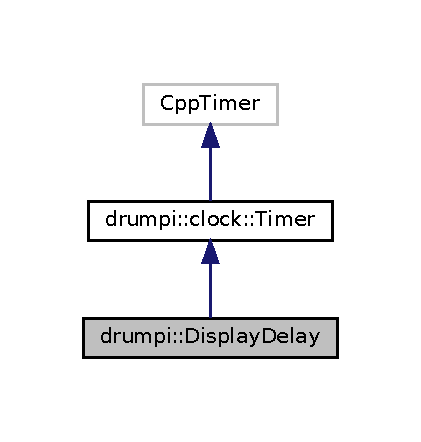
\includegraphics[width=202pt]{classdrumpi_1_1DisplayDelay__inherit__graph}
\end{center}
\end{figure}


Collaboration diagram for drumpi\+::Display\+Delay\+:\nopagebreak
\begin{figure}[H]
\begin{center}
\leavevmode
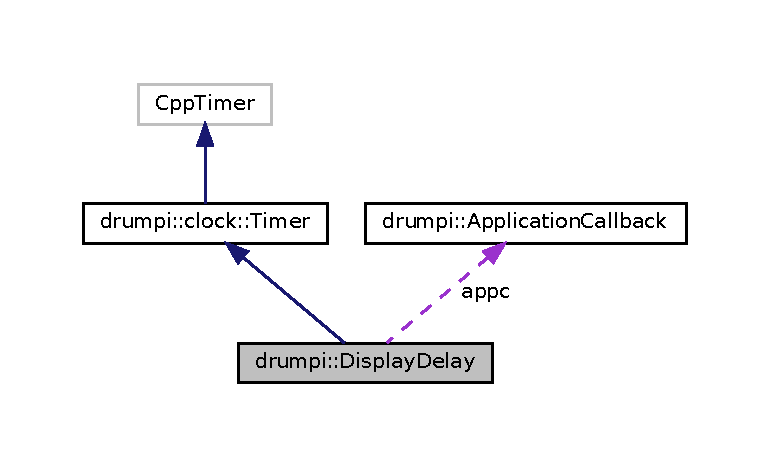
\includegraphics[width=350pt]{classdrumpi_1_1DisplayDelay__coll__graph}
\end{center}
\end{figure}
\doxysubsection*{Public Member Functions}
\begin{DoxyCompactItemize}
\item 
\mbox{\hyperlink{classdrumpi_1_1DisplayDelay_aefc2f9eeecfc90f2b03623104c457ed6}{Display\+Delay}} (\mbox{\hyperlink{classdrumpi_1_1ApplicationCallback}{Application\+Callback}} $\ast$a)
\item 
void \mbox{\hyperlink{classdrumpi_1_1DisplayDelay_a1fb66a57fea2d6700a190c961e556aa4}{trigger}} () override
\end{DoxyCompactItemize}
\doxysubsection*{Private Attributes}
\begin{DoxyCompactItemize}
\item 
\mbox{\hyperlink{classdrumpi_1_1ApplicationCallback}{Application\+Callback}} $\ast$ \mbox{\hyperlink{classdrumpi_1_1DisplayDelay_a1e0ae111b91375c8dd4de7310953728e}{appc}} = nullptr
\end{DoxyCompactItemize}


\doxysubsection{Detailed Description}
\mbox{\hyperlink{classdrumpi_1_1clock_1_1Timer_a5f16e8da27d2a5a5242dead46de05d97}{Timer}} derived class to clock master volume display timeout. 

\doxysubsection{Constructor \& Destructor Documentation}
\mbox{\Hypertarget{classdrumpi_1_1DisplayDelay_aefc2f9eeecfc90f2b03623104c457ed6}\label{classdrumpi_1_1DisplayDelay_aefc2f9eeecfc90f2b03623104c457ed6}} 
\index{drumpi::DisplayDelay@{drumpi::DisplayDelay}!DisplayDelay@{DisplayDelay}}
\index{DisplayDelay@{DisplayDelay}!drumpi::DisplayDelay@{drumpi::DisplayDelay}}
\doxysubsubsection{\texorpdfstring{DisplayDelay()}{DisplayDelay()}}
{\footnotesize\ttfamily Display\+Delay\+::\+Display\+Delay (\begin{DoxyParamCaption}\item[{\mbox{\hyperlink{classdrumpi_1_1ApplicationCallback}{Application\+Callback}} $\ast$}]{a }\end{DoxyParamCaption})}

Constructor. Sets the \mbox{\hyperlink{classdrumpi_1_1Application}{Application}} to be clocked. 
\begin{DoxyParams}{Parameters}
{\em a} & \mbox{\hyperlink{classdrumpi_1_1Application}{Application}} object to be clocked. \\
\hline
\end{DoxyParams}


\doxysubsection{Member Function Documentation}
\mbox{\Hypertarget{classdrumpi_1_1DisplayDelay_a1fb66a57fea2d6700a190c961e556aa4}\label{classdrumpi_1_1DisplayDelay_a1fb66a57fea2d6700a190c961e556aa4}} 
\index{drumpi::DisplayDelay@{drumpi::DisplayDelay}!trigger@{trigger}}
\index{trigger@{trigger}!drumpi::DisplayDelay@{drumpi::DisplayDelay}}
\doxysubsubsection{\texorpdfstring{trigger()}{trigger()}}
{\footnotesize\ttfamily void Display\+Delay\+::trigger (\begin{DoxyParamCaption}{ }\end{DoxyParamCaption})\hspace{0.3cm}{\ttfamily [override]}, {\ttfamily [virtual]}}

Override the tick method. Clocks the \mbox{\hyperlink{classdrumpi_1_1Application}{Application}}. 

Implements \mbox{\hyperlink{classdrumpi_1_1clock_1_1Timer_aeed4c4e653b98280354e0b970f8df68b}{drumpi\+::clock\+::\+Timer}}.



\doxysubsection{Member Data Documentation}
\mbox{\Hypertarget{classdrumpi_1_1DisplayDelay_a1e0ae111b91375c8dd4de7310953728e}\label{classdrumpi_1_1DisplayDelay_a1e0ae111b91375c8dd4de7310953728e}} 
\index{drumpi::DisplayDelay@{drumpi::DisplayDelay}!appc@{appc}}
\index{appc@{appc}!drumpi::DisplayDelay@{drumpi::DisplayDelay}}
\doxysubsubsection{\texorpdfstring{appc}{appc}}
{\footnotesize\ttfamily \mbox{\hyperlink{classdrumpi_1_1ApplicationCallback}{Application\+Callback}}$\ast$ drumpi\+::\+Display\+Delay\+::appc = nullptr\hspace{0.3cm}{\ttfamily [private]}}

Pointer to the {\ttfamily \mbox{\hyperlink{classdrumpi_1_1Application}{Application}}} object to be clocked. 

The documentation for this class was generated from the following files\+:\begin{DoxyCompactItemize}
\item 
src/application.\+hpp\item 
src/application.\+cpp\end{DoxyCompactItemize}

\hypertarget{classdrumpi_1_1audio_1_1JackClient}{}\section{drumpi\+:\+:audio\+:\+:Jack\+Client Class Reference}
\label{classdrumpi_1_1audio_1_1JackClient}\index{drumpi\+::audio\+::\+Jack\+Client@{drumpi\+::audio\+::\+Jack\+Client}}


{\ttfamily \#include $<$audio.\+hpp$>$}



Collaboration diagram for drumpi\+:\+:audio\+:\+:Jack\+Client\+:
\nopagebreak
\begin{figure}[H]
\begin{center}
\leavevmode
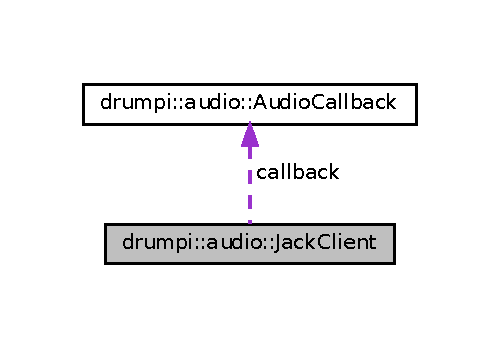
\includegraphics[width=224pt]{classdrumpi_1_1audio_1_1JackClient__coll__graph}
\end{center}
\end{figure}
\subsection*{Public Member Functions}
\begin{DoxyCompactItemize}
\item 
\hyperlink{classdrumpi_1_1audio_1_1JackClient_ab4cf3d533282d89dc9e1be8a64e22676}{Jack\+Client} (std\+::string \hyperlink{classdrumpi_1_1audio_1_1JackClient_a8b43d4d05f5afaeb3104b0b7f325688c}{client\+Name}, int n\+Out\+Ports=\hyperlink{classdrumpi_1_1audio_1_1JackClient_a4041995639d6765bb34dbadf27f7c3ec}{Jack\+Client\+::def\+Num\+Out\+Ports}, int n\+In\+Ports=\hyperlink{classdrumpi_1_1audio_1_1JackClient_abffcd237af5b33cb60bc93f4c0af3efa}{Jack\+Client\+::def\+Num\+In\+Ports})
\item 
\hyperlink{classdrumpi_1_1audio_1_1JackClient_ad9866ad3521128ca3a967aa96922ea97}{$\sim$\+Jack\+Client} ()
\item 
\hyperlink{namespacedrumpi_1_1audio_ac19e3be3b59052606a02605a7ee26f05}{audio\+Error\+\_\+t} \hyperlink{classdrumpi_1_1audio_1_1JackClient_ab76c081f0442dbe7ba23ab4715e11256}{start} (\hyperlink{classdrumpi_1_1audio_1_1AudioCallback}{Audio\+Callback} \&\hyperlink{classdrumpi_1_1audio_1_1JackClient_a607ea3c9f3b94f006db0abbf6382d6ac}{callback})
\item 
\hyperlink{namespacedrumpi_1_1audio_ac19e3be3b59052606a02605a7ee26f05}{audio\+Error\+\_\+t} \hyperlink{classdrumpi_1_1audio_1_1JackClient_aa4e28932809e94d3ee9ec02e19dac26d}{stop} (bool close\+Client=true)
\item 
bool \hyperlink{classdrumpi_1_1audio_1_1JackClient_a3b27776cda219ea706e77e96138b4c4e}{is\+Open} ()
\item 
bool \hyperlink{classdrumpi_1_1audio_1_1JackClient_ab5c76d2572a326d063761b6d8ec4d279}{is\+Running} ()
\end{DoxyCompactItemize}
\subsection*{Static Public Member Functions}
\begin{DoxyCompactItemize}
\item 
static int \hyperlink{classdrumpi_1_1audio_1_1JackClient_a70029f7ae102eba6b9b6a3160141d622}{\+\_\+process} (jack\+\_\+nframes\+\_\+t n\+Frames, void $\ast$arg)
\item 
static void \hyperlink{classdrumpi_1_1audio_1_1JackClient_ab3ec8c68b5c4473cdd3c53dc8f51b7c1}{\+\_\+shutdown} (void $\ast$arg)
\end{DoxyCompactItemize}
\subsection*{Private Member Functions}
\begin{DoxyCompactItemize}
\item 
void \hyperlink{classdrumpi_1_1audio_1_1JackClient_abb2363379d125b17299d49def97c289d}{set\+Num\+Ports} (int n\+Out\+Ports, int n\+In\+Ports)
\end{DoxyCompactItemize}
\subsection*{Private Attributes}
\begin{DoxyCompactItemize}
\item 
\hyperlink{classdrumpi_1_1audio_1_1AudioCallback}{Audio\+Callback} $\ast$ \hyperlink{classdrumpi_1_1audio_1_1JackClient_a607ea3c9f3b94f006db0abbf6382d6ac}{callback}
\item 
jack\+\_\+client\+\_\+t $\ast$ \hyperlink{classdrumpi_1_1audio_1_1JackClient_a7c7d354192fdfd02dff7ba19db35b055}{client}
\item 
std\+::string \hyperlink{classdrumpi_1_1audio_1_1JackClient_a8b43d4d05f5afaeb3104b0b7f325688c}{client\+Name}
\item 
std\+::vector$<$ jack\+\_\+port\+\_\+t $\ast$ $>$ \hyperlink{classdrumpi_1_1audio_1_1JackClient_a0257d5ed9aa2ad4a9c25776fa474f31e}{out\+Ports}
\item 
std\+::vector$<$ jack\+\_\+port\+\_\+t $\ast$ $>$ \hyperlink{classdrumpi_1_1audio_1_1JackClient_ac04a03af355ac3c7dd117ba8173b8d7a}{in\+Ports}
\item 
std\+::vector$<$ std\+::string $>$ \hyperlink{classdrumpi_1_1audio_1_1JackClient_ab90e744f9193a55d6543d117e9b6c00e}{ports}
\item 
jack\+\_\+options\+\_\+t \hyperlink{classdrumpi_1_1audio_1_1JackClient_ad2d5b25f8eceaad004f6f7058ec8e5b6}{options} = Jack\+Null\+Option
\item 
jack\+\_\+status\+\_\+t \hyperlink{classdrumpi_1_1audio_1_1JackClient_ae875ca9f70638eeb0ff80195634cb64b}{jack\+Status}
\item 
\hyperlink{namespacedrumpi_1_1audio_ac19e3be3b59052606a02605a7ee26f05}{audio\+Error\+\_\+t} \hyperlink{classdrumpi_1_1audio_1_1JackClient_a2bb52401891e1f4b9b74a5f347834f31}{error\+Status} = \hyperlink{namespacedrumpi_1_1audio_af36111ce9632c39e5acb2c811f228e2fa862613743b5354dc75cfa084840a7c0c}{N\+O\+\_\+\+E\+R\+R\+OR}
\item 
bool \hyperlink{classdrumpi_1_1audio_1_1JackClient_a827cedc289fc71939b040d757d15c65e}{open}
\item 
bool \hyperlink{classdrumpi_1_1audio_1_1JackClient_a087d17af8f6e68f1f609f3c276019a8e}{running}
\end{DoxyCompactItemize}
\subsection*{Static Private Attributes}
\begin{DoxyCompactItemize}
\item 
static const int \hyperlink{classdrumpi_1_1audio_1_1JackClient_a4041995639d6765bb34dbadf27f7c3ec}{def\+Num\+Out\+Ports} = 2
\item 
static const int \hyperlink{classdrumpi_1_1audio_1_1JackClient_abffcd237af5b33cb60bc93f4c0af3efa}{def\+Num\+In\+Ports} = 0
\end{DoxyCompactItemize}


\subsection{Detailed Description}
Audio engine class for interacting with the Jack server. 

\subsection{Constructor \& Destructor Documentation}
\mbox{\Hypertarget{classdrumpi_1_1audio_1_1JackClient_ab4cf3d533282d89dc9e1be8a64e22676}\label{classdrumpi_1_1audio_1_1JackClient_ab4cf3d533282d89dc9e1be8a64e22676}} 
\index{drumpi\+::audio\+::\+Jack\+Client@{drumpi\+::audio\+::\+Jack\+Client}!Jack\+Client@{Jack\+Client}}
\index{Jack\+Client@{Jack\+Client}!drumpi\+::audio\+::\+Jack\+Client@{drumpi\+::audio\+::\+Jack\+Client}}
\subsubsection{\texorpdfstring{Jack\+Client()}{JackClient()}}
{\footnotesize\ttfamily Jack\+Client\+::\+Jack\+Client (\begin{DoxyParamCaption}\item[{std\+::string}]{client\+Name,  }\item[{int}]{n\+Out\+Ports = {\ttfamily \hyperlink{classdrumpi_1_1audio_1_1JackClient_a4041995639d6765bb34dbadf27f7c3ec}{Jack\+Client\+::def\+Num\+Out\+Ports}},  }\item[{int}]{n\+In\+Ports = {\ttfamily \hyperlink{classdrumpi_1_1audio_1_1JackClient_abffcd237af5b33cb60bc93f4c0af3efa}{Jack\+Client\+::def\+Num\+In\+Ports}} }\end{DoxyParamCaption})}

Constructor. Specifies parameters to Jack. 
\begin{DoxyParams}{Parameters}
{\em client\+Name} & requested client name in Jack. \\
\hline
{\em n\+Out\+Ports} & number of output ports. Default 2. \\
\hline
{\em n\+In\+Ports} & number of input ports. Default 0. \\
\hline
\end{DoxyParams}
\mbox{\Hypertarget{classdrumpi_1_1audio_1_1JackClient_ad9866ad3521128ca3a967aa96922ea97}\label{classdrumpi_1_1audio_1_1JackClient_ad9866ad3521128ca3a967aa96922ea97}} 
\index{drumpi\+::audio\+::\+Jack\+Client@{drumpi\+::audio\+::\+Jack\+Client}!````~Jack\+Client@{$\sim$\+Jack\+Client}}
\index{````~Jack\+Client@{$\sim$\+Jack\+Client}!drumpi\+::audio\+::\+Jack\+Client@{drumpi\+::audio\+::\+Jack\+Client}}
\subsubsection{\texorpdfstring{$\sim$\+Jack\+Client()}{~JackClient()}}
{\footnotesize\ttfamily Jack\+Client\+::$\sim$\+Jack\+Client (\begin{DoxyParamCaption}{ }\end{DoxyParamCaption})}

Destructor. Closes the Jack client. 

\subsection{Member Function Documentation}
\mbox{\Hypertarget{classdrumpi_1_1audio_1_1JackClient_a70029f7ae102eba6b9b6a3160141d622}\label{classdrumpi_1_1audio_1_1JackClient_a70029f7ae102eba6b9b6a3160141d622}} 
\index{drumpi\+::audio\+::\+Jack\+Client@{drumpi\+::audio\+::\+Jack\+Client}!\+\_\+process@{\+\_\+process}}
\index{\+\_\+process@{\+\_\+process}!drumpi\+::audio\+::\+Jack\+Client@{drumpi\+::audio\+::\+Jack\+Client}}
\subsubsection{\texorpdfstring{\+\_\+process()}{\_process()}}
{\footnotesize\ttfamily int Jack\+Client\+::\+\_\+process (\begin{DoxyParamCaption}\item[{jack\+\_\+nframes\+\_\+t}]{n\+Frames,  }\item[{void $\ast$}]{arg }\end{DoxyParamCaption})\hspace{0.3cm}{\ttfamily [static]}}

Read method to send output buffer to the Jack server. Called by Jack when samples are needed. 
\begin{DoxyParams}{Parameters}
{\em n\+Frames} & number of frames requested by Jack. \\
\hline
{\em arg} & pointer to the \hyperlink{classdrumpi_1_1audio_1_1JackClient}{Jack\+Client} ({\ttfamily this}) object. \\
\hline
\end{DoxyParams}
\begin{DoxyReturn}{Returns}
Jack error code 
\end{DoxyReturn}
\mbox{\Hypertarget{classdrumpi_1_1audio_1_1JackClient_ab3ec8c68b5c4473cdd3c53dc8f51b7c1}\label{classdrumpi_1_1audio_1_1JackClient_ab3ec8c68b5c4473cdd3c53dc8f51b7c1}} 
\index{drumpi\+::audio\+::\+Jack\+Client@{drumpi\+::audio\+::\+Jack\+Client}!\+\_\+shutdown@{\+\_\+shutdown}}
\index{\+\_\+shutdown@{\+\_\+shutdown}!drumpi\+::audio\+::\+Jack\+Client@{drumpi\+::audio\+::\+Jack\+Client}}
\subsubsection{\texorpdfstring{\+\_\+shutdown()}{\_shutdown()}}
{\footnotesize\ttfamily void Jack\+Client\+::\+\_\+shutdown (\begin{DoxyParamCaption}\item[{void $\ast$}]{arg }\end{DoxyParamCaption})\hspace{0.3cm}{\ttfamily [static]}}

Shutdown method to exit the program should the Jack server shut down or disconnect the client. 
\begin{DoxyParams}{Parameters}
{\em arg} & 0. \\
\hline
\end{DoxyParams}
\mbox{\Hypertarget{classdrumpi_1_1audio_1_1JackClient_a3b27776cda219ea706e77e96138b4c4e}\label{classdrumpi_1_1audio_1_1JackClient_a3b27776cda219ea706e77e96138b4c4e}} 
\index{drumpi\+::audio\+::\+Jack\+Client@{drumpi\+::audio\+::\+Jack\+Client}!is\+Open@{is\+Open}}
\index{is\+Open@{is\+Open}!drumpi\+::audio\+::\+Jack\+Client@{drumpi\+::audio\+::\+Jack\+Client}}
\subsubsection{\texorpdfstring{is\+Open()}{isOpen()}}
{\footnotesize\ttfamily bool Jack\+Client\+::is\+Open (\begin{DoxyParamCaption}{ }\end{DoxyParamCaption})}

Check if the Jack client is open. \begin{DoxyReturn}{Returns}
{\ttfamily true} if the client is open. 
\end{DoxyReturn}
\mbox{\Hypertarget{classdrumpi_1_1audio_1_1JackClient_ab5c76d2572a326d063761b6d8ec4d279}\label{classdrumpi_1_1audio_1_1JackClient_ab5c76d2572a326d063761b6d8ec4d279}} 
\index{drumpi\+::audio\+::\+Jack\+Client@{drumpi\+::audio\+::\+Jack\+Client}!is\+Running@{is\+Running}}
\index{is\+Running@{is\+Running}!drumpi\+::audio\+::\+Jack\+Client@{drumpi\+::audio\+::\+Jack\+Client}}
\subsubsection{\texorpdfstring{is\+Running()}{isRunning()}}
{\footnotesize\ttfamily bool Jack\+Client\+::is\+Running (\begin{DoxyParamCaption}{ }\end{DoxyParamCaption})}

Check if the Jack client is running. \begin{DoxyReturn}{Returns}
{\ttfamily true} if the client is running. 
\end{DoxyReturn}
\mbox{\Hypertarget{classdrumpi_1_1audio_1_1JackClient_abb2363379d125b17299d49def97c289d}\label{classdrumpi_1_1audio_1_1JackClient_abb2363379d125b17299d49def97c289d}} 
\index{drumpi\+::audio\+::\+Jack\+Client@{drumpi\+::audio\+::\+Jack\+Client}!set\+Num\+Ports@{set\+Num\+Ports}}
\index{set\+Num\+Ports@{set\+Num\+Ports}!drumpi\+::audio\+::\+Jack\+Client@{drumpi\+::audio\+::\+Jack\+Client}}
\subsubsection{\texorpdfstring{set\+Num\+Ports()}{setNumPorts()}}
{\footnotesize\ttfamily void Jack\+Client\+::set\+Num\+Ports (\begin{DoxyParamCaption}\item[{int}]{n\+Out\+Ports,  }\item[{int}]{n\+In\+Ports }\end{DoxyParamCaption})\hspace{0.3cm}{\ttfamily [private]}}

Sets the number of Jack ports. 
\begin{DoxyParams}{Parameters}
{\em n\+Out\+Ports} & number of output ports. \\
\hline
{\em n\+In\+Ports} & number of input ports. \\
\hline
\end{DoxyParams}
\mbox{\Hypertarget{classdrumpi_1_1audio_1_1JackClient_ab76c081f0442dbe7ba23ab4715e11256}\label{classdrumpi_1_1audio_1_1JackClient_ab76c081f0442dbe7ba23ab4715e11256}} 
\index{drumpi\+::audio\+::\+Jack\+Client@{drumpi\+::audio\+::\+Jack\+Client}!start@{start}}
\index{start@{start}!drumpi\+::audio\+::\+Jack\+Client@{drumpi\+::audio\+::\+Jack\+Client}}
\subsubsection{\texorpdfstring{start()}{start()}}
{\footnotesize\ttfamily \hyperlink{namespacedrumpi_1_1audio_ac19e3be3b59052606a02605a7ee26f05}{audio\+Error\+\_\+t} Jack\+Client\+::start (\begin{DoxyParamCaption}\item[{\hyperlink{classdrumpi_1_1audio_1_1AudioCallback}{Audio\+Callback} \&}]{callback }\end{DoxyParamCaption})}

Informs Jack that the program is ready to go. 
\begin{DoxyParams}{Parameters}
{\em callback} & \hyperlink{classdrumpi_1_1audio_1_1AudioCallback}{Audio\+Callback} object to fetch output samples from. \\
\hline
\end{DoxyParams}
\begin{DoxyReturn}{Returns}
error code. 
\end{DoxyReturn}
\mbox{\Hypertarget{classdrumpi_1_1audio_1_1JackClient_aa4e28932809e94d3ee9ec02e19dac26d}\label{classdrumpi_1_1audio_1_1JackClient_aa4e28932809e94d3ee9ec02e19dac26d}} 
\index{drumpi\+::audio\+::\+Jack\+Client@{drumpi\+::audio\+::\+Jack\+Client}!stop@{stop}}
\index{stop@{stop}!drumpi\+::audio\+::\+Jack\+Client@{drumpi\+::audio\+::\+Jack\+Client}}
\subsubsection{\texorpdfstring{stop()}{stop()}}
{\footnotesize\ttfamily \hyperlink{namespacedrumpi_1_1audio_ac19e3be3b59052606a02605a7ee26f05}{audio\+Error\+\_\+t} Jack\+Client\+::stop (\begin{DoxyParamCaption}\item[{bool}]{close\+Client = {\ttfamily true} }\end{DoxyParamCaption})}

Stops the Jack engine. 
\begin{DoxyParams}{Parameters}
{\em close\+Client} & whether to close the Jack client or just deactivate it. \\
\hline
\end{DoxyParams}
\begin{DoxyReturn}{Returns}
error code. 
\end{DoxyReturn}


\subsection{Member Data Documentation}
\mbox{\Hypertarget{classdrumpi_1_1audio_1_1JackClient_a607ea3c9f3b94f006db0abbf6382d6ac}\label{classdrumpi_1_1audio_1_1JackClient_a607ea3c9f3b94f006db0abbf6382d6ac}} 
\index{drumpi\+::audio\+::\+Jack\+Client@{drumpi\+::audio\+::\+Jack\+Client}!callback@{callback}}
\index{callback@{callback}!drumpi\+::audio\+::\+Jack\+Client@{drumpi\+::audio\+::\+Jack\+Client}}
\subsubsection{\texorpdfstring{callback}{callback}}
{\footnotesize\ttfamily \hyperlink{classdrumpi_1_1audio_1_1AudioCallback}{Audio\+Callback}$\ast$ drumpi\+::audio\+::\+Jack\+Client\+::callback\hspace{0.3cm}{\ttfamily [private]}}

Pointer to the \hyperlink{classdrumpi_1_1audio_1_1AudioCallback}{Audio\+Callback} object that fetches output samples. \mbox{\Hypertarget{classdrumpi_1_1audio_1_1JackClient_a7c7d354192fdfd02dff7ba19db35b055}\label{classdrumpi_1_1audio_1_1JackClient_a7c7d354192fdfd02dff7ba19db35b055}} 
\index{drumpi\+::audio\+::\+Jack\+Client@{drumpi\+::audio\+::\+Jack\+Client}!client@{client}}
\index{client@{client}!drumpi\+::audio\+::\+Jack\+Client@{drumpi\+::audio\+::\+Jack\+Client}}
\subsubsection{\texorpdfstring{client}{client}}
{\footnotesize\ttfamily jack\+\_\+client\+\_\+t$\ast$ drumpi\+::audio\+::\+Jack\+Client\+::client\hspace{0.3cm}{\ttfamily [private]}}

Pointer to the Jack client. \mbox{\Hypertarget{classdrumpi_1_1audio_1_1JackClient_a8b43d4d05f5afaeb3104b0b7f325688c}\label{classdrumpi_1_1audio_1_1JackClient_a8b43d4d05f5afaeb3104b0b7f325688c}} 
\index{drumpi\+::audio\+::\+Jack\+Client@{drumpi\+::audio\+::\+Jack\+Client}!client\+Name@{client\+Name}}
\index{client\+Name@{client\+Name}!drumpi\+::audio\+::\+Jack\+Client@{drumpi\+::audio\+::\+Jack\+Client}}
\subsubsection{\texorpdfstring{client\+Name}{clientName}}
{\footnotesize\ttfamily std\+::string drumpi\+::audio\+::\+Jack\+Client\+::client\+Name\hspace{0.3cm}{\ttfamily [private]}}

Jack client name. \mbox{\Hypertarget{classdrumpi_1_1audio_1_1JackClient_abffcd237af5b33cb60bc93f4c0af3efa}\label{classdrumpi_1_1audio_1_1JackClient_abffcd237af5b33cb60bc93f4c0af3efa}} 
\index{drumpi\+::audio\+::\+Jack\+Client@{drumpi\+::audio\+::\+Jack\+Client}!def\+Num\+In\+Ports@{def\+Num\+In\+Ports}}
\index{def\+Num\+In\+Ports@{def\+Num\+In\+Ports}!drumpi\+::audio\+::\+Jack\+Client@{drumpi\+::audio\+::\+Jack\+Client}}
\subsubsection{\texorpdfstring{def\+Num\+In\+Ports}{defNumInPorts}}
{\footnotesize\ttfamily const int drumpi\+::audio\+::\+Jack\+Client\+::def\+Num\+In\+Ports = 0\hspace{0.3cm}{\ttfamily [static]}, {\ttfamily [private]}}

Default number of input ports. \mbox{\Hypertarget{classdrumpi_1_1audio_1_1JackClient_a4041995639d6765bb34dbadf27f7c3ec}\label{classdrumpi_1_1audio_1_1JackClient_a4041995639d6765bb34dbadf27f7c3ec}} 
\index{drumpi\+::audio\+::\+Jack\+Client@{drumpi\+::audio\+::\+Jack\+Client}!def\+Num\+Out\+Ports@{def\+Num\+Out\+Ports}}
\index{def\+Num\+Out\+Ports@{def\+Num\+Out\+Ports}!drumpi\+::audio\+::\+Jack\+Client@{drumpi\+::audio\+::\+Jack\+Client}}
\subsubsection{\texorpdfstring{def\+Num\+Out\+Ports}{defNumOutPorts}}
{\footnotesize\ttfamily const int drumpi\+::audio\+::\+Jack\+Client\+::def\+Num\+Out\+Ports = 2\hspace{0.3cm}{\ttfamily [static]}, {\ttfamily [private]}}

Default number of output ports. \mbox{\Hypertarget{classdrumpi_1_1audio_1_1JackClient_a2bb52401891e1f4b9b74a5f347834f31}\label{classdrumpi_1_1audio_1_1JackClient_a2bb52401891e1f4b9b74a5f347834f31}} 
\index{drumpi\+::audio\+::\+Jack\+Client@{drumpi\+::audio\+::\+Jack\+Client}!error\+Status@{error\+Status}}
\index{error\+Status@{error\+Status}!drumpi\+::audio\+::\+Jack\+Client@{drumpi\+::audio\+::\+Jack\+Client}}
\subsubsection{\texorpdfstring{error\+Status}{errorStatus}}
{\footnotesize\ttfamily \hyperlink{namespacedrumpi_1_1audio_ac19e3be3b59052606a02605a7ee26f05}{audio\+Error\+\_\+t} drumpi\+::audio\+::\+Jack\+Client\+::error\+Status = \hyperlink{namespacedrumpi_1_1audio_af36111ce9632c39e5acb2c811f228e2fa862613743b5354dc75cfa084840a7c0c}{N\+O\+\_\+\+E\+R\+R\+OR}\hspace{0.3cm}{\ttfamily [private]}}

\hyperlink{classdrumpi_1_1audio_1_1JackClient}{Jack\+Client} error status. \mbox{\Hypertarget{classdrumpi_1_1audio_1_1JackClient_ac04a03af355ac3c7dd117ba8173b8d7a}\label{classdrumpi_1_1audio_1_1JackClient_ac04a03af355ac3c7dd117ba8173b8d7a}} 
\index{drumpi\+::audio\+::\+Jack\+Client@{drumpi\+::audio\+::\+Jack\+Client}!in\+Ports@{in\+Ports}}
\index{in\+Ports@{in\+Ports}!drumpi\+::audio\+::\+Jack\+Client@{drumpi\+::audio\+::\+Jack\+Client}}
\subsubsection{\texorpdfstring{in\+Ports}{inPorts}}
{\footnotesize\ttfamily std\+::vector$<$jack\+\_\+port\+\_\+t$\ast$$>$ drumpi\+::audio\+::\+Jack\+Client\+::in\+Ports\hspace{0.3cm}{\ttfamily [private]}}

Jack input ports. Not (yet) implemented. \mbox{\Hypertarget{classdrumpi_1_1audio_1_1JackClient_ae875ca9f70638eeb0ff80195634cb64b}\label{classdrumpi_1_1audio_1_1JackClient_ae875ca9f70638eeb0ff80195634cb64b}} 
\index{drumpi\+::audio\+::\+Jack\+Client@{drumpi\+::audio\+::\+Jack\+Client}!jack\+Status@{jack\+Status}}
\index{jack\+Status@{jack\+Status}!drumpi\+::audio\+::\+Jack\+Client@{drumpi\+::audio\+::\+Jack\+Client}}
\subsubsection{\texorpdfstring{jack\+Status}{jackStatus}}
{\footnotesize\ttfamily jack\+\_\+status\+\_\+t drumpi\+::audio\+::\+Jack\+Client\+::jack\+Status\hspace{0.3cm}{\ttfamily [private]}}

Jack status. \mbox{\Hypertarget{classdrumpi_1_1audio_1_1JackClient_a827cedc289fc71939b040d757d15c65e}\label{classdrumpi_1_1audio_1_1JackClient_a827cedc289fc71939b040d757d15c65e}} 
\index{drumpi\+::audio\+::\+Jack\+Client@{drumpi\+::audio\+::\+Jack\+Client}!open@{open}}
\index{open@{open}!drumpi\+::audio\+::\+Jack\+Client@{drumpi\+::audio\+::\+Jack\+Client}}
\subsubsection{\texorpdfstring{open}{open}}
{\footnotesize\ttfamily bool drumpi\+::audio\+::\+Jack\+Client\+::open\hspace{0.3cm}{\ttfamily [private]}}

Jack client open status. \mbox{\Hypertarget{classdrumpi_1_1audio_1_1JackClient_ad2d5b25f8eceaad004f6f7058ec8e5b6}\label{classdrumpi_1_1audio_1_1JackClient_ad2d5b25f8eceaad004f6f7058ec8e5b6}} 
\index{drumpi\+::audio\+::\+Jack\+Client@{drumpi\+::audio\+::\+Jack\+Client}!options@{options}}
\index{options@{options}!drumpi\+::audio\+::\+Jack\+Client@{drumpi\+::audio\+::\+Jack\+Client}}
\subsubsection{\texorpdfstring{options}{options}}
{\footnotesize\ttfamily jack\+\_\+options\+\_\+t drumpi\+::audio\+::\+Jack\+Client\+::options = Jack\+Null\+Option\hspace{0.3cm}{\ttfamily [private]}}

Jack options. \mbox{\Hypertarget{classdrumpi_1_1audio_1_1JackClient_a0257d5ed9aa2ad4a9c25776fa474f31e}\label{classdrumpi_1_1audio_1_1JackClient_a0257d5ed9aa2ad4a9c25776fa474f31e}} 
\index{drumpi\+::audio\+::\+Jack\+Client@{drumpi\+::audio\+::\+Jack\+Client}!out\+Ports@{out\+Ports}}
\index{out\+Ports@{out\+Ports}!drumpi\+::audio\+::\+Jack\+Client@{drumpi\+::audio\+::\+Jack\+Client}}
\subsubsection{\texorpdfstring{out\+Ports}{outPorts}}
{\footnotesize\ttfamily std\+::vector$<$jack\+\_\+port\+\_\+t$\ast$$>$ drumpi\+::audio\+::\+Jack\+Client\+::out\+Ports\hspace{0.3cm}{\ttfamily [private]}}

Jack output ports. \mbox{\Hypertarget{classdrumpi_1_1audio_1_1JackClient_ab90e744f9193a55d6543d117e9b6c00e}\label{classdrumpi_1_1audio_1_1JackClient_ab90e744f9193a55d6543d117e9b6c00e}} 
\index{drumpi\+::audio\+::\+Jack\+Client@{drumpi\+::audio\+::\+Jack\+Client}!ports@{ports}}
\index{ports@{ports}!drumpi\+::audio\+::\+Jack\+Client@{drumpi\+::audio\+::\+Jack\+Client}}
\subsubsection{\texorpdfstring{ports}{ports}}
{\footnotesize\ttfamily std\+::vector$<$std\+::string$>$ drumpi\+::audio\+::\+Jack\+Client\+::ports\hspace{0.3cm}{\ttfamily [private]}}

Jack ports string. \mbox{\Hypertarget{classdrumpi_1_1audio_1_1JackClient_a087d17af8f6e68f1f609f3c276019a8e}\label{classdrumpi_1_1audio_1_1JackClient_a087d17af8f6e68f1f609f3c276019a8e}} 
\index{drumpi\+::audio\+::\+Jack\+Client@{drumpi\+::audio\+::\+Jack\+Client}!running@{running}}
\index{running@{running}!drumpi\+::audio\+::\+Jack\+Client@{drumpi\+::audio\+::\+Jack\+Client}}
\subsubsection{\texorpdfstring{running}{running}}
{\footnotesize\ttfamily bool drumpi\+::audio\+::\+Jack\+Client\+::running\hspace{0.3cm}{\ttfamily [private]}}

Jack client running status. 

The documentation for this class was generated from the following files\+:\begin{DoxyCompactItemize}
\item 
src/audio.\+hpp\item 
src/audio.\+cpp\end{DoxyCompactItemize}

\hypertarget{classdrumpi_1_1KeyboardInput}{}\section{drumpi\+:\+:Keyboard\+Input Class Reference}
\label{classdrumpi_1_1KeyboardInput}\index{drumpi\+::\+Keyboard\+Input@{drumpi\+::\+Keyboard\+Input}}


{\ttfamily \#include $<$keyboardinput.\+hpp$>$}



Collaboration diagram for drumpi\+:\+:Keyboard\+Input\+:
\nopagebreak
\begin{figure}[H]
\begin{center}
\leavevmode
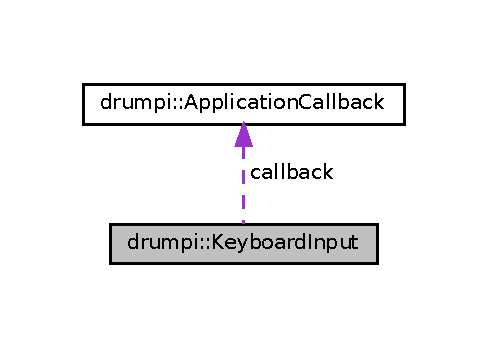
\includegraphics[width=218pt]{classdrumpi_1_1KeyboardInput__coll__graph}
\end{center}
\end{figure}
\subsection*{Public Member Functions}
\begin{DoxyCompactItemize}
\item 
\hyperlink{classdrumpi_1_1KeyboardInput_a92d9c25232e73f2d9319c79df028cc69}{Keyboard\+Input} ()
\begin{DoxyCompactList}\small\item\em Constructor. \end{DoxyCompactList}\item 
void \hyperlink{classdrumpi_1_1KeyboardInput_ac74a81a24054aa5e927e03b4ba7f8c9f}{poll\+Input} ()
\begin{DoxyCompactList}\small\item\em Polls the keyboard input for events. \end{DoxyCompactList}\item 
void \hyperlink{classdrumpi_1_1KeyboardInput_acd7e27115fbb3b81bc3d1b771ef89ca8}{connect\+Callback} (\hyperlink{classdrumpi_1_1ApplicationCallback}{Application\+Callback} $\ast$app)
\begin{DoxyCompactList}\small\item\em Sets the \hyperlink{classdrumpi_1_1Application}{Application} object called when a keyboard event occurs. \end{DoxyCompactList}\item 
int \hyperlink{classdrumpi_1_1KeyboardInput_a9541bb7ef3f3c78c448e7b18aec1dbd7}{get\+File\+Descriptor} ()
\item 
int \hyperlink{classdrumpi_1_1KeyboardInput_a657e489023c7fe835a53d7b24c1eec39}{get\+Test\+Flag} ()
\end{DoxyCompactItemize}
\subsection*{Public Attributes}
\begin{DoxyCompactItemize}
\item 
int \hyperlink{classdrumpi_1_1KeyboardInput_a92b9933a95405da091d18b8b3116699b}{running}
\item 
\hyperlink{classdrumpi_1_1ApplicationCallback}{Application\+Callback} $\ast$ \hyperlink{classdrumpi_1_1KeyboardInput_a7af8c85eed4c1997ae9b56ac5bf2a7e1}{callback}
\end{DoxyCompactItemize}
\subsection*{Private Attributes}
\begin{DoxyCompactItemize}
\item 
struct input\+\_\+event \hyperlink{classdrumpi_1_1KeyboardInput_a2b530250c3bb5d744611671e430e283d}{ev}
\item 
struct pollfd \hyperlink{classdrumpi_1_1KeyboardInput_a94851cf204554afc60046d39a265c4e7}{fdset} \mbox{[}1\mbox{]}
\item 
int \hyperlink{classdrumpi_1_1KeyboardInput_a098990e43175ae8a2ad64e6d3b487c83}{fd}
\item 
int \hyperlink{classdrumpi_1_1KeyboardInput_a1817959cdce29597ad61ba635674bc6f}{test\+Flag}
\end{DoxyCompactItemize}


\subsection{Detailed Description}
Class for monitoring a keyboard device file and detecting keyboard presses. 

\subsection{Constructor \& Destructor Documentation}
\mbox{\Hypertarget{classdrumpi_1_1KeyboardInput_a92d9c25232e73f2d9319c79df028cc69}\label{classdrumpi_1_1KeyboardInput_a92d9c25232e73f2d9319c79df028cc69}} 
\index{drumpi\+::\+Keyboard\+Input@{drumpi\+::\+Keyboard\+Input}!Keyboard\+Input@{Keyboard\+Input}}
\index{Keyboard\+Input@{Keyboard\+Input}!drumpi\+::\+Keyboard\+Input@{drumpi\+::\+Keyboard\+Input}}
\subsubsection{\texorpdfstring{Keyboard\+Input()}{KeyboardInput()}}
{\footnotesize\ttfamily Keyboard\+Input\+::\+Keyboard\+Input (\begin{DoxyParamCaption}{ }\end{DoxyParamCaption})}



Constructor. 

The constructor detects and opens the device file for the keyboard input device. 

\subsection{Member Function Documentation}
\mbox{\Hypertarget{classdrumpi_1_1KeyboardInput_acd7e27115fbb3b81bc3d1b771ef89ca8}\label{classdrumpi_1_1KeyboardInput_acd7e27115fbb3b81bc3d1b771ef89ca8}} 
\index{drumpi\+::\+Keyboard\+Input@{drumpi\+::\+Keyboard\+Input}!connect\+Callback@{connect\+Callback}}
\index{connect\+Callback@{connect\+Callback}!drumpi\+::\+Keyboard\+Input@{drumpi\+::\+Keyboard\+Input}}
\subsubsection{\texorpdfstring{connect\+Callback()}{connectCallback()}}
{\footnotesize\ttfamily void Keyboard\+Input\+::connect\+Callback (\begin{DoxyParamCaption}\item[{\hyperlink{classdrumpi_1_1ApplicationCallback}{Application\+Callback} $\ast$}]{app }\end{DoxyParamCaption})}



Sets the \hyperlink{classdrumpi_1_1Application}{Application} object called when a keyboard event occurs. 


\begin{DoxyParams}{Parameters}
{\em app} & \hyperlink{classdrumpi_1_1Application}{Application} object called by poll\+Input when a key press is detected. \\
\hline
\end{DoxyParams}
\mbox{\Hypertarget{classdrumpi_1_1KeyboardInput_a9541bb7ef3f3c78c448e7b18aec1dbd7}\label{classdrumpi_1_1KeyboardInput_a9541bb7ef3f3c78c448e7b18aec1dbd7}} 
\index{drumpi\+::\+Keyboard\+Input@{drumpi\+::\+Keyboard\+Input}!get\+File\+Descriptor@{get\+File\+Descriptor}}
\index{get\+File\+Descriptor@{get\+File\+Descriptor}!drumpi\+::\+Keyboard\+Input@{drumpi\+::\+Keyboard\+Input}}
\subsubsection{\texorpdfstring{get\+File\+Descriptor()}{getFileDescriptor()}}
{\footnotesize\ttfamily int Keyboard\+Input\+::get\+File\+Descriptor (\begin{DoxyParamCaption}{ }\end{DoxyParamCaption})}

\begin{DoxyReturn}{Returns}
file descriptor \hyperlink{classdrumpi_1_1KeyboardInput_a098990e43175ae8a2ad64e6d3b487c83}{fd} of the input device. 
\end{DoxyReturn}
\mbox{\Hypertarget{classdrumpi_1_1KeyboardInput_a657e489023c7fe835a53d7b24c1eec39}\label{classdrumpi_1_1KeyboardInput_a657e489023c7fe835a53d7b24c1eec39}} 
\index{drumpi\+::\+Keyboard\+Input@{drumpi\+::\+Keyboard\+Input}!get\+Test\+Flag@{get\+Test\+Flag}}
\index{get\+Test\+Flag@{get\+Test\+Flag}!drumpi\+::\+Keyboard\+Input@{drumpi\+::\+Keyboard\+Input}}
\subsubsection{\texorpdfstring{get\+Test\+Flag()}{getTestFlag()}}
{\footnotesize\ttfamily int Keyboard\+Input\+::get\+Test\+Flag (\begin{DoxyParamCaption}{ }\end{DoxyParamCaption})}

\begin{DoxyReturn}{Returns}
\hyperlink{classdrumpi_1_1KeyboardInput_a1817959cdce29597ad61ba635674bc6f}{test\+Flag}. 
\end{DoxyReturn}
\mbox{\Hypertarget{classdrumpi_1_1KeyboardInput_ac74a81a24054aa5e927e03b4ba7f8c9f}\label{classdrumpi_1_1KeyboardInput_ac74a81a24054aa5e927e03b4ba7f8c9f}} 
\index{drumpi\+::\+Keyboard\+Input@{drumpi\+::\+Keyboard\+Input}!poll\+Input@{poll\+Input}}
\index{poll\+Input@{poll\+Input}!drumpi\+::\+Keyboard\+Input@{drumpi\+::\+Keyboard\+Input}}
\subsubsection{\texorpdfstring{poll\+Input()}{pollInput()}}
{\footnotesize\ttfamily void Keyboard\+Input\+::poll\+Input (\begin{DoxyParamCaption}{ }\end{DoxyParamCaption})}



Polls the keyboard input for events. 

This method monitors the keyboard device file with a polling loop and calls the \hyperlink{classdrumpi_1_1Application}{Application} object to interpret the key press and perform an action when a key press is detected. 

\subsection{Member Data Documentation}
\mbox{\Hypertarget{classdrumpi_1_1KeyboardInput_a7af8c85eed4c1997ae9b56ac5bf2a7e1}\label{classdrumpi_1_1KeyboardInput_a7af8c85eed4c1997ae9b56ac5bf2a7e1}} 
\index{drumpi\+::\+Keyboard\+Input@{drumpi\+::\+Keyboard\+Input}!callback@{callback}}
\index{callback@{callback}!drumpi\+::\+Keyboard\+Input@{drumpi\+::\+Keyboard\+Input}}
\subsubsection{\texorpdfstring{callback}{callback}}
{\footnotesize\ttfamily \hyperlink{classdrumpi_1_1ApplicationCallback}{Application\+Callback}$\ast$ drumpi\+::\+Keyboard\+Input\+::callback}

Callback class called by \hyperlink{classdrumpi_1_1KeyboardInput}{Keyboard\+Input} when a keyboard event occurs. \mbox{\Hypertarget{classdrumpi_1_1KeyboardInput_a2b530250c3bb5d744611671e430e283d}\label{classdrumpi_1_1KeyboardInput_a2b530250c3bb5d744611671e430e283d}} 
\index{drumpi\+::\+Keyboard\+Input@{drumpi\+::\+Keyboard\+Input}!ev@{ev}}
\index{ev@{ev}!drumpi\+::\+Keyboard\+Input@{drumpi\+::\+Keyboard\+Input}}
\subsubsection{\texorpdfstring{ev}{ev}}
{\footnotesize\ttfamily struct input\+\_\+event drumpi\+::\+Keyboard\+Input\+::ev\hspace{0.3cm}{\ttfamily [private]}}

Event handler containing information about keyboard input events. \mbox{\Hypertarget{classdrumpi_1_1KeyboardInput_a098990e43175ae8a2ad64e6d3b487c83}\label{classdrumpi_1_1KeyboardInput_a098990e43175ae8a2ad64e6d3b487c83}} 
\index{drumpi\+::\+Keyboard\+Input@{drumpi\+::\+Keyboard\+Input}!fd@{fd}}
\index{fd@{fd}!drumpi\+::\+Keyboard\+Input@{drumpi\+::\+Keyboard\+Input}}
\subsubsection{\texorpdfstring{fd}{fd}}
{\footnotesize\ttfamily int drumpi\+::\+Keyboard\+Input\+::fd\hspace{0.3cm}{\ttfamily [private]}}

File descriptor for the keyboard device file. \mbox{\Hypertarget{classdrumpi_1_1KeyboardInput_a94851cf204554afc60046d39a265c4e7}\label{classdrumpi_1_1KeyboardInput_a94851cf204554afc60046d39a265c4e7}} 
\index{drumpi\+::\+Keyboard\+Input@{drumpi\+::\+Keyboard\+Input}!fdset@{fdset}}
\index{fdset@{fdset}!drumpi\+::\+Keyboard\+Input@{drumpi\+::\+Keyboard\+Input}}
\subsubsection{\texorpdfstring{fdset}{fdset}}
{\footnotesize\ttfamily struct pollfd drumpi\+::\+Keyboard\+Input\+::fdset\mbox{[}1\mbox{]}\hspace{0.3cm}{\ttfamily [private]}}

Array of pollfd structs checked by poll() system call. \mbox{\Hypertarget{classdrumpi_1_1KeyboardInput_a92b9933a95405da091d18b8b3116699b}\label{classdrumpi_1_1KeyboardInput_a92b9933a95405da091d18b8b3116699b}} 
\index{drumpi\+::\+Keyboard\+Input@{drumpi\+::\+Keyboard\+Input}!running@{running}}
\index{running@{running}!drumpi\+::\+Keyboard\+Input@{drumpi\+::\+Keyboard\+Input}}
\subsubsection{\texorpdfstring{running}{running}}
{\footnotesize\ttfamily int drumpi\+::\+Keyboard\+Input\+::running}

Running flag used to end the input polling loop. \mbox{\Hypertarget{classdrumpi_1_1KeyboardInput_a1817959cdce29597ad61ba635674bc6f}\label{classdrumpi_1_1KeyboardInput_a1817959cdce29597ad61ba635674bc6f}} 
\index{drumpi\+::\+Keyboard\+Input@{drumpi\+::\+Keyboard\+Input}!test\+Flag@{test\+Flag}}
\index{test\+Flag@{test\+Flag}!drumpi\+::\+Keyboard\+Input@{drumpi\+::\+Keyboard\+Input}}
\subsubsection{\texorpdfstring{test\+Flag}{testFlag}}
{\footnotesize\ttfamily int drumpi\+::\+Keyboard\+Input\+::test\+Flag\hspace{0.3cm}{\ttfamily [private]}}

Flag to check \hyperlink{classdrumpi_1_1KeyboardInput_ac74a81a24054aa5e927e03b4ba7f8c9f}{poll\+Input} has been called successfully. 

The documentation for this class was generated from the following files\+:\begin{DoxyCompactItemize}
\item 
src/keyboardinput.\+hpp\item 
src/keyboardinput.\+cpp\end{DoxyCompactItemize}

\hypertarget{classdrumpi_1_1KeyboardThread}{}\section{drumpi\+:\+:Keyboard\+Thread Class Reference}
\label{classdrumpi_1_1KeyboardThread}\index{drumpi\+::\+Keyboard\+Thread@{drumpi\+::\+Keyboard\+Thread}}


{\ttfamily \#include $<$keyboardthread.\+hpp$>$}



Inheritance diagram for drumpi\+:\+:Keyboard\+Thread\+:
\nopagebreak
\begin{figure}[H]
\begin{center}
\leavevmode
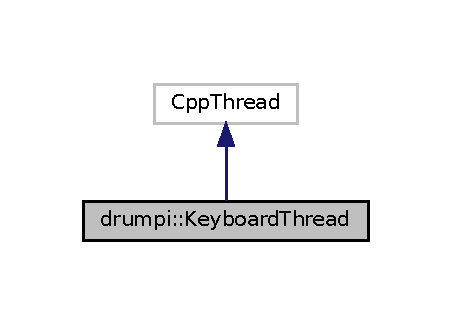
\includegraphics[width=203pt]{classdrumpi_1_1KeyboardThread__inherit__graph}
\end{center}
\end{figure}


Collaboration diagram for drumpi\+:\+:Keyboard\+Thread\+:
\nopagebreak
\begin{figure}[H]
\begin{center}
\leavevmode
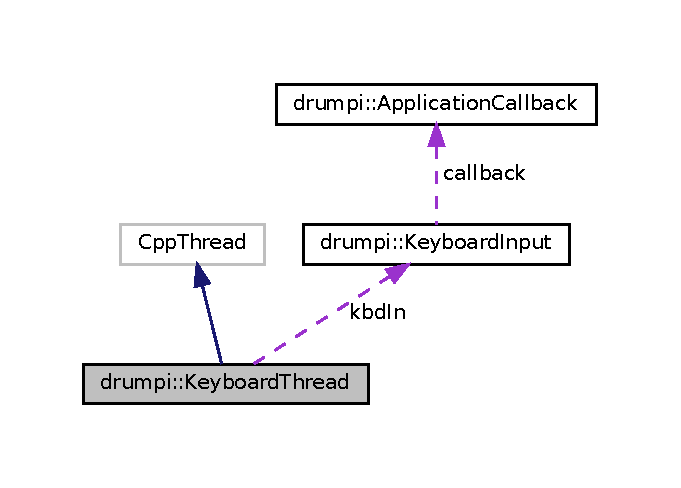
\includegraphics[width=290pt]{classdrumpi_1_1KeyboardThread__coll__graph}
\end{center}
\end{figure}
\subsection*{Public Member Functions}
\begin{DoxyCompactItemize}
\item 
int \hyperlink{classdrumpi_1_1KeyboardThread_a2e106118779a9a70aabf9c291c2f9a36}{stop} ()
\item 
void \hyperlink{classdrumpi_1_1KeyboardThread_a406ee901b3d40676ba070548b3ac7d12}{run} ()
\end{DoxyCompactItemize}
\subsection*{Public Attributes}
\begin{DoxyCompactItemize}
\item 
\hyperlink{classdrumpi_1_1KeyboardInput}{Keyboard\+Input} \hyperlink{classdrumpi_1_1KeyboardThread_a2f248c78ba5f7bcd0f4db0fc3050ef4d}{kbd\+In}
\end{DoxyCompactItemize}


\subsection{Detailed Description}
This class inherits from the Cpp\+Thread wrapper class and creates a keyboard monitoring thread. 

\subsection{Member Function Documentation}
\mbox{\Hypertarget{classdrumpi_1_1KeyboardThread_a406ee901b3d40676ba070548b3ac7d12}\label{classdrumpi_1_1KeyboardThread_a406ee901b3d40676ba070548b3ac7d12}} 
\index{drumpi\+::\+Keyboard\+Thread@{drumpi\+::\+Keyboard\+Thread}!run@{run}}
\index{run@{run}!drumpi\+::\+Keyboard\+Thread@{drumpi\+::\+Keyboard\+Thread}}
\subsubsection{\texorpdfstring{run()}{run()}}
{\footnotesize\ttfamily void Keyboard\+Thread\+::run (\begin{DoxyParamCaption}{ }\end{DoxyParamCaption})}

This method is called when the thread is started. \mbox{\Hypertarget{classdrumpi_1_1KeyboardThread_a2e106118779a9a70aabf9c291c2f9a36}\label{classdrumpi_1_1KeyboardThread_a2e106118779a9a70aabf9c291c2f9a36}} 
\index{drumpi\+::\+Keyboard\+Thread@{drumpi\+::\+Keyboard\+Thread}!stop@{stop}}
\index{stop@{stop}!drumpi\+::\+Keyboard\+Thread@{drumpi\+::\+Keyboard\+Thread}}
\subsubsection{\texorpdfstring{stop()}{stop()}}
{\footnotesize\ttfamily int Keyboard\+Thread\+::stop (\begin{DoxyParamCaption}{ }\end{DoxyParamCaption})}

Closes the thread. 

\subsection{Member Data Documentation}
\mbox{\Hypertarget{classdrumpi_1_1KeyboardThread_a2f248c78ba5f7bcd0f4db0fc3050ef4d}\label{classdrumpi_1_1KeyboardThread_a2f248c78ba5f7bcd0f4db0fc3050ef4d}} 
\index{drumpi\+::\+Keyboard\+Thread@{drumpi\+::\+Keyboard\+Thread}!kbd\+In@{kbd\+In}}
\index{kbd\+In@{kbd\+In}!drumpi\+::\+Keyboard\+Thread@{drumpi\+::\+Keyboard\+Thread}}
\subsubsection{\texorpdfstring{kbd\+In}{kbdIn}}
{\footnotesize\ttfamily \hyperlink{classdrumpi_1_1KeyboardInput}{Keyboard\+Input} drumpi\+::\+Keyboard\+Thread\+::kbd\+In}

Instance of \hyperlink{classdrumpi_1_1KeyboardInput}{Keyboard\+Input} class. 

The documentation for this class was generated from the following files\+:\begin{DoxyCompactItemize}
\item 
src/keyboardthread.\+hpp\item 
src/keyboardthread.\+cpp\end{DoxyCompactItemize}

\hypertarget{classdrumpi_1_1Max7219}{}\doxysection{drumpi\+::Max7219 Class Reference}
\label{classdrumpi_1_1Max7219}\index{drumpi::Max7219@{drumpi::Max7219}}


{\ttfamily \#include $<$display.\+hpp$>$}



Inheritance diagram for drumpi\+::Max7219\+:\nopagebreak
\begin{figure}[H]
\begin{center}
\leavevmode
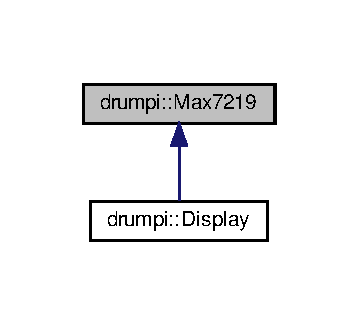
\includegraphics[width=182pt]{classdrumpi_1_1Max7219__inherit__graph}
\end{center}
\end{figure}
\doxysubsection*{Public Member Functions}
\begin{DoxyCompactItemize}
\item 
\mbox{\hyperlink{classdrumpi_1_1Max7219_abc709f2a3b36fb872c560398b980aeb6}{Max7219}} (unsigned char \mbox{\hyperlink{classdrumpi_1_1Max7219_a7ba5a789cdd1120814595b89ba4e99e0}{decode\+Mode}}=0x0, unsigned char \mbox{\hyperlink{classdrumpi_1_1Max7219_a22aa789cc1ac84c6c5df7ad59607afed}{intensity}}=0x7, unsigned char \mbox{\hyperlink{classdrumpi_1_1Max7219_a605af97de38c0f8fd581ba17e6ce4f37}{scan\+Limit}}=0x7, unsigned char \mbox{\hyperlink{classdrumpi_1_1Max7219_a0b1b2c31442fe9a3a1db3cdae5dd32e8}{shutdown}}=0x1, unsigned char \mbox{\hyperlink{classdrumpi_1_1Max7219_a203552d0f41ceb1366dbd8bbf1608110}{display\+Test}}=0x0, unsigned int \mbox{\hyperlink{classdrumpi_1_1Max7219_a71d7054477a82db272fb5c584576f25a}{num\+Digits}}=8)
\item 
\mbox{\hyperlink{classdrumpi_1_1Max7219_a47402da87a159c0fbe04b3a9cb5668f1}{$\sim$\+Max7219}} ()
\item 
void \mbox{\hyperlink{classdrumpi_1_1Max7219_ad85d8d612e1c7a817da7d18bd9f336da}{set\+Digit}} (unsigned char digit, unsigned char value, bool redraw)
\item 
void \mbox{\hyperlink{classdrumpi_1_1Max7219_a237f07a9f87919651cc30cb5afacbc7d}{set\+Decode\+Mode}} (unsigned char value)
\item 
void \mbox{\hyperlink{classdrumpi_1_1Max7219_a7a722668b9b1d232792f6877171ca7c5}{set\+Intensity}} (unsigned char value)
\item 
void \mbox{\hyperlink{classdrumpi_1_1Max7219_a2d13fd1c5a05004cb69dbaef8f1fed3a}{set\+Scan\+Limit}} (unsigned char value)
\item 
void \mbox{\hyperlink{classdrumpi_1_1Max7219_a7b4ded1ec0a564ef12fb1ed4fd45bd1c}{set\+Shutdown}} (unsigned char value)
\item 
void \mbox{\hyperlink{classdrumpi_1_1Max7219_a1f1e7b7c538c539854ad5901e6bba3fe}{set\+Display\+Test}} (unsigned char value)
\item 
unsigned char \mbox{\hyperlink{classdrumpi_1_1Max7219_a30e98c660745c63d883696589b0e4f4f}{get\+Digit}} (unsigned char digit)
\item 
unsigned char \mbox{\hyperlink{classdrumpi_1_1Max7219_a78fc1bac71f62e85657a224f23af2189}{get\+Decode\+Mode}} ()
\item 
unsigned char \mbox{\hyperlink{classdrumpi_1_1Max7219_a16035185e3439775135256e40ad638a9}{get\+Intensity}} ()
\item 
unsigned char \mbox{\hyperlink{classdrumpi_1_1Max7219_a3ec0ff91fa65b1d6a1c435b15cb4604e}{get\+Scan\+Limit}} ()
\item 
unsigned char \mbox{\hyperlink{classdrumpi_1_1Max7219_af2a8322c6ac792793fd9b2c6d7f389fd}{get\+Shutdown}} ()
\item 
unsigned char \mbox{\hyperlink{classdrumpi_1_1Max7219_aec71032f6aff755a3cf1a45183dceb96}{get\+Display\+Test}} ()
\item 
unsigned int \mbox{\hyperlink{classdrumpi_1_1Max7219_ab6bc447965dffdc63f050b2eda80cedd}{get\+Num\+Digits}} ()
\item 
void \mbox{\hyperlink{classdrumpi_1_1Max7219_a3b3f0f2a947caf27f65bd626f8e71f43}{flush}} ()
\item 
void \mbox{\hyperlink{classdrumpi_1_1Max7219_ac29e3df34f72833d995db8bc1810f04d}{clear}} (bool redraw)
\end{DoxyCompactItemize}
\doxysubsection*{Private Member Functions}
\begin{DoxyCompactItemize}
\item 
void \mbox{\hyperlink{classdrumpi_1_1Max7219_aaf2f49b227cb65ead3ce0811714fe592}{write}} (unsigned char $\ast$data, unsigned int len)
\item 
void \mbox{\hyperlink{classdrumpi_1_1Max7219_a45fe4b7d187a021dca6c75ad7319ed6f}{command}} (unsigned char reg, unsigned char data)
\end{DoxyCompactItemize}
\doxysubsection*{Private Attributes}
\begin{DoxyCompactItemize}
\item 
unsigned int \mbox{\hyperlink{classdrumpi_1_1Max7219_a71d7054477a82db272fb5c584576f25a}{num\+Digits}}
\item 
unsigned char \mbox{\hyperlink{classdrumpi_1_1Max7219_a7ba5a789cdd1120814595b89ba4e99e0}{decode\+Mode}}
\item 
unsigned char \mbox{\hyperlink{classdrumpi_1_1Max7219_a22aa789cc1ac84c6c5df7ad59607afed}{intensity}}
\item 
unsigned char \mbox{\hyperlink{classdrumpi_1_1Max7219_a605af97de38c0f8fd581ba17e6ce4f37}{scan\+Limit}}
\item 
unsigned char \mbox{\hyperlink{classdrumpi_1_1Max7219_a0b1b2c31442fe9a3a1db3cdae5dd32e8}{shutdown}}
\item 
unsigned char \mbox{\hyperlink{classdrumpi_1_1Max7219_a203552d0f41ceb1366dbd8bbf1608110}{display\+Test}}
\item 
std\+::vector$<$ unsigned char $>$ \mbox{\hyperlink{classdrumpi_1_1Max7219_ab26f32728dd82c00e39b6212436f291e}{digit\+Buffer}}
\end{DoxyCompactItemize}


\doxysubsection{Detailed Description}
Low level driver for the \mbox{\hyperlink{classdrumpi_1_1Max7219}{Max7219}} 7-\/segment display driver 

\doxysubsection{Constructor \& Destructor Documentation}
\mbox{\Hypertarget{classdrumpi_1_1Max7219_abc709f2a3b36fb872c560398b980aeb6}\label{classdrumpi_1_1Max7219_abc709f2a3b36fb872c560398b980aeb6}} 
\index{drumpi::Max7219@{drumpi::Max7219}!Max7219@{Max7219}}
\index{Max7219@{Max7219}!drumpi::Max7219@{drumpi::Max7219}}
\doxysubsubsection{\texorpdfstring{Max7219()}{Max7219()}}
{\footnotesize\ttfamily Max7219\+::\+Max7219 (\begin{DoxyParamCaption}\item[{unsigned char}]{decode\+Mode = {\ttfamily 0x0},  }\item[{unsigned char}]{intensity = {\ttfamily 0x7},  }\item[{unsigned char}]{scan\+Limit = {\ttfamily 0x7},  }\item[{unsigned char}]{shutdown = {\ttfamily 0x1},  }\item[{unsigned char}]{display\+Test = {\ttfamily 0x0},  }\item[{unsigned int}]{num\+Digits = {\ttfamily 8} }\end{DoxyParamCaption})}

Constructor


\begin{DoxyParams}{Parameters}
{\em decode\+Mode} & decode mode to be set. (default 0x0) \\
\hline
{\em intensity} & Intensity to be set. (default 0x7) \\
\hline
{\em scan\+Limit} & Scan Limit to be set. (default 0x7) \\
\hline
{\em shutdown} & Shutdown mode to be set. (default 0x1) \\
\hline
{\em display\+Test} & \mbox{\hyperlink{classdrumpi_1_1Display}{Display}} test mode to be set. (default 0x0) \\
\hline
{\em num\+Digits} & Number of digits in display. (default 8) \\
\hline
\end{DoxyParams}
\mbox{\Hypertarget{classdrumpi_1_1Max7219_a47402da87a159c0fbe04b3a9cb5668f1}\label{classdrumpi_1_1Max7219_a47402da87a159c0fbe04b3a9cb5668f1}} 
\index{drumpi::Max7219@{drumpi::Max7219}!````~Max7219@{$\sim$Max7219}}
\index{````~Max7219@{$\sim$Max7219}!drumpi::Max7219@{drumpi::Max7219}}
\doxysubsubsection{\texorpdfstring{$\sim$Max7219()}{~Max7219()}}
{\footnotesize\ttfamily Max7219\+::$\sim$\+Max7219 (\begin{DoxyParamCaption}{ }\end{DoxyParamCaption})}

Destructor -\/ deletes any allocated memory and clears display. 

\doxysubsection{Member Function Documentation}
\mbox{\Hypertarget{classdrumpi_1_1Max7219_ac29e3df34f72833d995db8bc1810f04d}\label{classdrumpi_1_1Max7219_ac29e3df34f72833d995db8bc1810f04d}} 
\index{drumpi::Max7219@{drumpi::Max7219}!clear@{clear}}
\index{clear@{clear}!drumpi::Max7219@{drumpi::Max7219}}
\doxysubsubsection{\texorpdfstring{clear()}{clear()}}
{\footnotesize\ttfamily void Max7219\+::clear (\begin{DoxyParamCaption}\item[{bool}]{redraw }\end{DoxyParamCaption})}

Resets all digits in the \mbox{\hyperlink{classdrumpi_1_1Max7219_ab26f32728dd82c00e39b6212436f291e}{digit\+Buffer}} to 0. 
\begin{DoxyParams}{Parameters}
{\em redraw} & If true, calls \mbox{\hyperlink{classdrumpi_1_1Max7219_a3b3f0f2a947caf27f65bd626f8e71f43}{flush}} to update display. \\
\hline
\end{DoxyParams}
\mbox{\Hypertarget{classdrumpi_1_1Max7219_a45fe4b7d187a021dca6c75ad7319ed6f}\label{classdrumpi_1_1Max7219_a45fe4b7d187a021dca6c75ad7319ed6f}} 
\index{drumpi::Max7219@{drumpi::Max7219}!command@{command}}
\index{command@{command}!drumpi::Max7219@{drumpi::Max7219}}
\doxysubsubsection{\texorpdfstring{command()}{command()}}
{\footnotesize\ttfamily void Max7219\+::command (\begin{DoxyParamCaption}\item[{unsigned char}]{reg,  }\item[{unsigned char}]{data }\end{DoxyParamCaption})\hspace{0.3cm}{\ttfamily [private]}}

Sends command data over S\+PI bus. \mbox{\Hypertarget{classdrumpi_1_1Max7219_a3b3f0f2a947caf27f65bd626f8e71f43}\label{classdrumpi_1_1Max7219_a3b3f0f2a947caf27f65bd626f8e71f43}} 
\index{drumpi::Max7219@{drumpi::Max7219}!flush@{flush}}
\index{flush@{flush}!drumpi::Max7219@{drumpi::Max7219}}
\doxysubsubsection{\texorpdfstring{flush()}{flush()}}
{\footnotesize\ttfamily void Max7219\+::flush (\begin{DoxyParamCaption}{ }\end{DoxyParamCaption})}

Writes all \mbox{\hyperlink{classdrumpi_1_1Max7219_ab26f32728dd82c00e39b6212436f291e}{digit\+Buffer}} values to display via S\+PI bus. \mbox{\Hypertarget{classdrumpi_1_1Max7219_a78fc1bac71f62e85657a224f23af2189}\label{classdrumpi_1_1Max7219_a78fc1bac71f62e85657a224f23af2189}} 
\index{drumpi::Max7219@{drumpi::Max7219}!getDecodeMode@{getDecodeMode}}
\index{getDecodeMode@{getDecodeMode}!drumpi::Max7219@{drumpi::Max7219}}
\doxysubsubsection{\texorpdfstring{getDecodeMode()}{getDecodeMode()}}
{\footnotesize\ttfamily unsigned char Max7219\+::get\+Decode\+Mode (\begin{DoxyParamCaption}{ }\end{DoxyParamCaption})}

Gets the current \mbox{\hyperlink{classdrumpi_1_1Max7219_a7ba5a789cdd1120814595b89ba4e99e0}{decode\+Mode}}. \begin{DoxyReturn}{Returns}
Current \mbox{\hyperlink{classdrumpi_1_1Max7219_a7ba5a789cdd1120814595b89ba4e99e0}{decode\+Mode}}. 
\end{DoxyReturn}
\mbox{\Hypertarget{classdrumpi_1_1Max7219_a30e98c660745c63d883696589b0e4f4f}\label{classdrumpi_1_1Max7219_a30e98c660745c63d883696589b0e4f4f}} 
\index{drumpi::Max7219@{drumpi::Max7219}!getDigit@{getDigit}}
\index{getDigit@{getDigit}!drumpi::Max7219@{drumpi::Max7219}}
\doxysubsubsection{\texorpdfstring{getDigit()}{getDigit()}}
{\footnotesize\ttfamily unsigned char Max7219\+::get\+Digit (\begin{DoxyParamCaption}\item[{unsigned char}]{digit }\end{DoxyParamCaption})}

Gets a value of a digit in the \mbox{\hyperlink{classdrumpi_1_1Max7219_ab26f32728dd82c00e39b6212436f291e}{digit\+Buffer}}. 
\begin{DoxyParams}{Parameters}
{\em digit} & Byte address of digit. \\
\hline
\end{DoxyParams}
\begin{DoxyReturn}{Returns}
Current byte value of digit. 
\end{DoxyReturn}
\mbox{\Hypertarget{classdrumpi_1_1Max7219_aec71032f6aff755a3cf1a45183dceb96}\label{classdrumpi_1_1Max7219_aec71032f6aff755a3cf1a45183dceb96}} 
\index{drumpi::Max7219@{drumpi::Max7219}!getDisplayTest@{getDisplayTest}}
\index{getDisplayTest@{getDisplayTest}!drumpi::Max7219@{drumpi::Max7219}}
\doxysubsubsection{\texorpdfstring{getDisplayTest()}{getDisplayTest()}}
{\footnotesize\ttfamily unsigned char Max7219\+::get\+Display\+Test (\begin{DoxyParamCaption}{ }\end{DoxyParamCaption})}

Gets the current \mbox{\hyperlink{classdrumpi_1_1Max7219_a203552d0f41ceb1366dbd8bbf1608110}{display\+Test}} mode. \begin{DoxyReturn}{Returns}
Current \mbox{\hyperlink{classdrumpi_1_1Max7219_a203552d0f41ceb1366dbd8bbf1608110}{display\+Test}} mode. 
\end{DoxyReturn}
\mbox{\Hypertarget{classdrumpi_1_1Max7219_a16035185e3439775135256e40ad638a9}\label{classdrumpi_1_1Max7219_a16035185e3439775135256e40ad638a9}} 
\index{drumpi::Max7219@{drumpi::Max7219}!getIntensity@{getIntensity}}
\index{getIntensity@{getIntensity}!drumpi::Max7219@{drumpi::Max7219}}
\doxysubsubsection{\texorpdfstring{getIntensity()}{getIntensity()}}
{\footnotesize\ttfamily unsigned char Max7219\+::get\+Intensity (\begin{DoxyParamCaption}{ }\end{DoxyParamCaption})}

Gets the current \mbox{\hyperlink{classdrumpi_1_1Max7219_a22aa789cc1ac84c6c5df7ad59607afed}{intensity}}. \begin{DoxyReturn}{Returns}
Current \mbox{\hyperlink{classdrumpi_1_1Max7219_a22aa789cc1ac84c6c5df7ad59607afed}{intensity}}. 
\end{DoxyReturn}
\mbox{\Hypertarget{classdrumpi_1_1Max7219_ab6bc447965dffdc63f050b2eda80cedd}\label{classdrumpi_1_1Max7219_ab6bc447965dffdc63f050b2eda80cedd}} 
\index{drumpi::Max7219@{drumpi::Max7219}!getNumDigits@{getNumDigits}}
\index{getNumDigits@{getNumDigits}!drumpi::Max7219@{drumpi::Max7219}}
\doxysubsubsection{\texorpdfstring{getNumDigits()}{getNumDigits()}}
{\footnotesize\ttfamily unsigned int Max7219\+::get\+Num\+Digits (\begin{DoxyParamCaption}{ }\end{DoxyParamCaption})}

Gets the number of digits in the display. \begin{DoxyReturn}{Returns}
Number of display digits. 
\end{DoxyReturn}
\mbox{\Hypertarget{classdrumpi_1_1Max7219_a3ec0ff91fa65b1d6a1c435b15cb4604e}\label{classdrumpi_1_1Max7219_a3ec0ff91fa65b1d6a1c435b15cb4604e}} 
\index{drumpi::Max7219@{drumpi::Max7219}!getScanLimit@{getScanLimit}}
\index{getScanLimit@{getScanLimit}!drumpi::Max7219@{drumpi::Max7219}}
\doxysubsubsection{\texorpdfstring{getScanLimit()}{getScanLimit()}}
{\footnotesize\ttfamily unsigned char Max7219\+::get\+Scan\+Limit (\begin{DoxyParamCaption}{ }\end{DoxyParamCaption})}

Gets the current \mbox{\hyperlink{classdrumpi_1_1Max7219_a605af97de38c0f8fd581ba17e6ce4f37}{scan\+Limit}}. \begin{DoxyReturn}{Returns}
Current \mbox{\hyperlink{classdrumpi_1_1Max7219_a605af97de38c0f8fd581ba17e6ce4f37}{scan\+Limit}}. 
\end{DoxyReturn}
\mbox{\Hypertarget{classdrumpi_1_1Max7219_af2a8322c6ac792793fd9b2c6d7f389fd}\label{classdrumpi_1_1Max7219_af2a8322c6ac792793fd9b2c6d7f389fd}} 
\index{drumpi::Max7219@{drumpi::Max7219}!getShutdown@{getShutdown}}
\index{getShutdown@{getShutdown}!drumpi::Max7219@{drumpi::Max7219}}
\doxysubsubsection{\texorpdfstring{getShutdown()}{getShutdown()}}
{\footnotesize\ttfamily unsigned char Max7219\+::get\+Shutdown (\begin{DoxyParamCaption}{ }\end{DoxyParamCaption})}

Gets the current \mbox{\hyperlink{classdrumpi_1_1Max7219_a0b1b2c31442fe9a3a1db3cdae5dd32e8}{shutdown}} mode. \begin{DoxyReturn}{Returns}
Current \mbox{\hyperlink{classdrumpi_1_1Max7219_a0b1b2c31442fe9a3a1db3cdae5dd32e8}{shutdown}} mode. 
\end{DoxyReturn}
\mbox{\Hypertarget{classdrumpi_1_1Max7219_a237f07a9f87919651cc30cb5afacbc7d}\label{classdrumpi_1_1Max7219_a237f07a9f87919651cc30cb5afacbc7d}} 
\index{drumpi::Max7219@{drumpi::Max7219}!setDecodeMode@{setDecodeMode}}
\index{setDecodeMode@{setDecodeMode}!drumpi::Max7219@{drumpi::Max7219}}
\doxysubsubsection{\texorpdfstring{setDecodeMode()}{setDecodeMode()}}
{\footnotesize\ttfamily void Max7219\+::set\+Decode\+Mode (\begin{DoxyParamCaption}\item[{unsigned char}]{value }\end{DoxyParamCaption})}

Sets the \mbox{\hyperlink{classdrumpi_1_1Max7219_a7ba5a789cdd1120814595b89ba4e99e0}{decode\+Mode}}. 
\begin{DoxyParams}{Parameters}
{\em value} & Decode mode byte. \\
\hline
\end{DoxyParams}
\mbox{\Hypertarget{classdrumpi_1_1Max7219_ad85d8d612e1c7a817da7d18bd9f336da}\label{classdrumpi_1_1Max7219_ad85d8d612e1c7a817da7d18bd9f336da}} 
\index{drumpi::Max7219@{drumpi::Max7219}!setDigit@{setDigit}}
\index{setDigit@{setDigit}!drumpi::Max7219@{drumpi::Max7219}}
\doxysubsubsection{\texorpdfstring{setDigit()}{setDigit()}}
{\footnotesize\ttfamily void Max7219\+::set\+Digit (\begin{DoxyParamCaption}\item[{unsigned char}]{digit,  }\item[{unsigned char}]{value,  }\item[{bool}]{redraw }\end{DoxyParamCaption})}

Sets a value in the \mbox{\hyperlink{classdrumpi_1_1Max7219_ab26f32728dd82c00e39b6212436f291e}{digit\+Buffer}}.


\begin{DoxyParams}{Parameters}
{\em digit} & Byte address of digit. \\
\hline
{\em value} & Byte value to assign. \\
\hline
{\em redraw} & If true, updates all digits at the end of method call. \\
\hline
\end{DoxyParams}
\mbox{\Hypertarget{classdrumpi_1_1Max7219_a1f1e7b7c538c539854ad5901e6bba3fe}\label{classdrumpi_1_1Max7219_a1f1e7b7c538c539854ad5901e6bba3fe}} 
\index{drumpi::Max7219@{drumpi::Max7219}!setDisplayTest@{setDisplayTest}}
\index{setDisplayTest@{setDisplayTest}!drumpi::Max7219@{drumpi::Max7219}}
\doxysubsubsection{\texorpdfstring{setDisplayTest()}{setDisplayTest()}}
{\footnotesize\ttfamily void Max7219\+::set\+Display\+Test (\begin{DoxyParamCaption}\item[{unsigned char}]{value }\end{DoxyParamCaption})}

Sets the \mbox{\hyperlink{classdrumpi_1_1Max7219_a203552d0f41ceb1366dbd8bbf1608110}{display\+Test}} mode. 
\begin{DoxyParams}{Parameters}
{\em value} & \mbox{\hyperlink{classdrumpi_1_1Display}{Display}} test mode (1/0). \\
\hline
\end{DoxyParams}
\mbox{\Hypertarget{classdrumpi_1_1Max7219_a7a722668b9b1d232792f6877171ca7c5}\label{classdrumpi_1_1Max7219_a7a722668b9b1d232792f6877171ca7c5}} 
\index{drumpi::Max7219@{drumpi::Max7219}!setIntensity@{setIntensity}}
\index{setIntensity@{setIntensity}!drumpi::Max7219@{drumpi::Max7219}}
\doxysubsubsection{\texorpdfstring{setIntensity()}{setIntensity()}}
{\footnotesize\ttfamily void Max7219\+::set\+Intensity (\begin{DoxyParamCaption}\item[{unsigned char}]{value }\end{DoxyParamCaption})}

Sets the \mbox{\hyperlink{classdrumpi_1_1Max7219_a22aa789cc1ac84c6c5df7ad59607afed}{intensity}}. 
\begin{DoxyParams}{Parameters}
{\em value} & Intensity value (1-\/15). \\
\hline
\end{DoxyParams}
\mbox{\Hypertarget{classdrumpi_1_1Max7219_a2d13fd1c5a05004cb69dbaef8f1fed3a}\label{classdrumpi_1_1Max7219_a2d13fd1c5a05004cb69dbaef8f1fed3a}} 
\index{drumpi::Max7219@{drumpi::Max7219}!setScanLimit@{setScanLimit}}
\index{setScanLimit@{setScanLimit}!drumpi::Max7219@{drumpi::Max7219}}
\doxysubsubsection{\texorpdfstring{setScanLimit()}{setScanLimit()}}
{\footnotesize\ttfamily void Max7219\+::set\+Scan\+Limit (\begin{DoxyParamCaption}\item[{unsigned char}]{value }\end{DoxyParamCaption})}

Sets the \mbox{\hyperlink{classdrumpi_1_1Max7219_a605af97de38c0f8fd581ba17e6ce4f37}{scan\+Limit}}. 
\begin{DoxyParams}{Parameters}
{\em value} & Scan limit (0-\/7). \\
\hline
\end{DoxyParams}
\mbox{\Hypertarget{classdrumpi_1_1Max7219_a7b4ded1ec0a564ef12fb1ed4fd45bd1c}\label{classdrumpi_1_1Max7219_a7b4ded1ec0a564ef12fb1ed4fd45bd1c}} 
\index{drumpi::Max7219@{drumpi::Max7219}!setShutdown@{setShutdown}}
\index{setShutdown@{setShutdown}!drumpi::Max7219@{drumpi::Max7219}}
\doxysubsubsection{\texorpdfstring{setShutdown()}{setShutdown()}}
{\footnotesize\ttfamily void Max7219\+::set\+Shutdown (\begin{DoxyParamCaption}\item[{unsigned char}]{value }\end{DoxyParamCaption})}

Sets the \mbox{\hyperlink{classdrumpi_1_1Max7219_a0b1b2c31442fe9a3a1db3cdae5dd32e8}{shutdown}} mode. 
\begin{DoxyParams}{Parameters}
{\em value} & Shutdown mode (1/0). \\
\hline
\end{DoxyParams}
\mbox{\Hypertarget{classdrumpi_1_1Max7219_aaf2f49b227cb65ead3ce0811714fe592}\label{classdrumpi_1_1Max7219_aaf2f49b227cb65ead3ce0811714fe592}} 
\index{drumpi::Max7219@{drumpi::Max7219}!write@{write}}
\index{write@{write}!drumpi::Max7219@{drumpi::Max7219}}
\doxysubsubsection{\texorpdfstring{write()}{write()}}
{\footnotesize\ttfamily void Max7219\+::write (\begin{DoxyParamCaption}\item[{unsigned char $\ast$}]{data,  }\item[{unsigned int}]{len }\end{DoxyParamCaption})\hspace{0.3cm}{\ttfamily [private]}}

Low level method for writing a data buffer to S\+PI bus. Should not be used by host application. Instead use \mbox{\hyperlink{classdrumpi_1_1Max7219_ad85d8d612e1c7a817da7d18bd9f336da}{set\+Digit}} and \mbox{\hyperlink{classdrumpi_1_1Max7219_a3b3f0f2a947caf27f65bd626f8e71f43}{flush}} methods.


\begin{DoxyParams}{Parameters}
{\em data} & Buffer containing bytes for writing. \\
\hline
{\em len} & Length of buffer in bytes. \\
\hline
\end{DoxyParams}


\doxysubsection{Member Data Documentation}
\mbox{\Hypertarget{classdrumpi_1_1Max7219_a7ba5a789cdd1120814595b89ba4e99e0}\label{classdrumpi_1_1Max7219_a7ba5a789cdd1120814595b89ba4e99e0}} 
\index{drumpi::Max7219@{drumpi::Max7219}!decodeMode@{decodeMode}}
\index{decodeMode@{decodeMode}!drumpi::Max7219@{drumpi::Max7219}}
\doxysubsubsection{\texorpdfstring{decodeMode}{decodeMode}}
{\footnotesize\ttfamily unsigned char drumpi\+::\+Max7219\+::decode\+Mode\hspace{0.3cm}{\ttfamily [private]}}

\mbox{\hyperlink{classdrumpi_1_1Display}{Display}} decode mode. \mbox{\Hypertarget{classdrumpi_1_1Max7219_ab26f32728dd82c00e39b6212436f291e}\label{classdrumpi_1_1Max7219_ab26f32728dd82c00e39b6212436f291e}} 
\index{drumpi::Max7219@{drumpi::Max7219}!digitBuffer@{digitBuffer}}
\index{digitBuffer@{digitBuffer}!drumpi::Max7219@{drumpi::Max7219}}
\doxysubsubsection{\texorpdfstring{digitBuffer}{digitBuffer}}
{\footnotesize\ttfamily std\+::vector$<$unsigned char$>$ drumpi\+::\+Max7219\+::digit\+Buffer\hspace{0.3cm}{\ttfamily [private]}}

Buffer to contain each digit\textquotesingle{}s value. \mbox{\Hypertarget{classdrumpi_1_1Max7219_a203552d0f41ceb1366dbd8bbf1608110}\label{classdrumpi_1_1Max7219_a203552d0f41ceb1366dbd8bbf1608110}} 
\index{drumpi::Max7219@{drumpi::Max7219}!displayTest@{displayTest}}
\index{displayTest@{displayTest}!drumpi::Max7219@{drumpi::Max7219}}
\doxysubsubsection{\texorpdfstring{displayTest}{displayTest}}
{\footnotesize\ttfamily unsigned char drumpi\+::\+Max7219\+::display\+Test\hspace{0.3cm}{\ttfamily [private]}}

\mbox{\hyperlink{classdrumpi_1_1Display}{Display}} display test mode. \mbox{\Hypertarget{classdrumpi_1_1Max7219_a22aa789cc1ac84c6c5df7ad59607afed}\label{classdrumpi_1_1Max7219_a22aa789cc1ac84c6c5df7ad59607afed}} 
\index{drumpi::Max7219@{drumpi::Max7219}!intensity@{intensity}}
\index{intensity@{intensity}!drumpi::Max7219@{drumpi::Max7219}}
\doxysubsubsection{\texorpdfstring{intensity}{intensity}}
{\footnotesize\ttfamily unsigned char drumpi\+::\+Max7219\+::intensity\hspace{0.3cm}{\ttfamily [private]}}

\mbox{\hyperlink{classdrumpi_1_1Display}{Display}} intensity. \mbox{\Hypertarget{classdrumpi_1_1Max7219_a71d7054477a82db272fb5c584576f25a}\label{classdrumpi_1_1Max7219_a71d7054477a82db272fb5c584576f25a}} 
\index{drumpi::Max7219@{drumpi::Max7219}!numDigits@{numDigits}}
\index{numDigits@{numDigits}!drumpi::Max7219@{drumpi::Max7219}}
\doxysubsubsection{\texorpdfstring{numDigits}{numDigits}}
{\footnotesize\ttfamily unsigned int drumpi\+::\+Max7219\+::num\+Digits\hspace{0.3cm}{\ttfamily [private]}}

Number of digits. \mbox{\Hypertarget{classdrumpi_1_1Max7219_a605af97de38c0f8fd581ba17e6ce4f37}\label{classdrumpi_1_1Max7219_a605af97de38c0f8fd581ba17e6ce4f37}} 
\index{drumpi::Max7219@{drumpi::Max7219}!scanLimit@{scanLimit}}
\index{scanLimit@{scanLimit}!drumpi::Max7219@{drumpi::Max7219}}
\doxysubsubsection{\texorpdfstring{scanLimit}{scanLimit}}
{\footnotesize\ttfamily unsigned char drumpi\+::\+Max7219\+::scan\+Limit\hspace{0.3cm}{\ttfamily [private]}}

\mbox{\hyperlink{classdrumpi_1_1Display}{Display}} scan limit. \mbox{\Hypertarget{classdrumpi_1_1Max7219_a0b1b2c31442fe9a3a1db3cdae5dd32e8}\label{classdrumpi_1_1Max7219_a0b1b2c31442fe9a3a1db3cdae5dd32e8}} 
\index{drumpi::Max7219@{drumpi::Max7219}!shutdown@{shutdown}}
\index{shutdown@{shutdown}!drumpi::Max7219@{drumpi::Max7219}}
\doxysubsubsection{\texorpdfstring{shutdown}{shutdown}}
{\footnotesize\ttfamily unsigned char drumpi\+::\+Max7219\+::shutdown\hspace{0.3cm}{\ttfamily [private]}}

\mbox{\hyperlink{classdrumpi_1_1Display}{Display}} shutdown mode. 

The documentation for this class was generated from the following files\+:\begin{DoxyCompactItemize}
\item 
src/display.\+hpp\item 
src/display.\+cpp\end{DoxyCompactItemize}

\hypertarget{classdrumpi_1_1clock_1_1Metronome}{}\section{drumpi\+:\+:clock\+:\+:Metronome Class Reference}
\label{classdrumpi_1_1clock_1_1Metronome}\index{drumpi\+::clock\+::\+Metronome@{drumpi\+::clock\+::\+Metronome}}


{\ttfamily \#include $<$clock.\+hpp$>$}



Inheritance diagram for drumpi\+:\+:clock\+:\+:Metronome\+:
\nopagebreak
\begin{figure}[H]
\begin{center}
\leavevmode
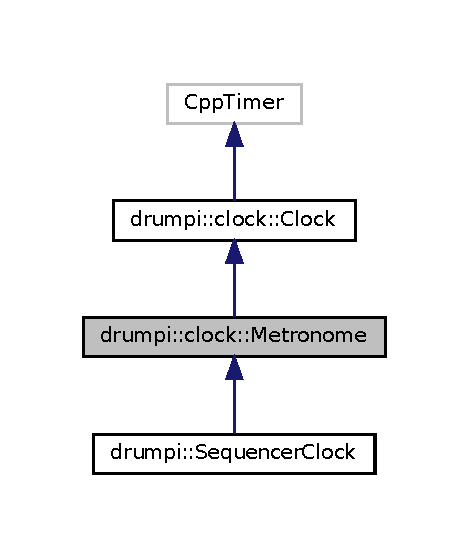
\includegraphics[width=210pt]{classdrumpi_1_1clock_1_1Metronome__inherit__graph}
\end{center}
\end{figure}


Collaboration diagram for drumpi\+:\+:clock\+:\+:Metronome\+:
\nopagebreak
\begin{figure}[H]
\begin{center}
\leavevmode
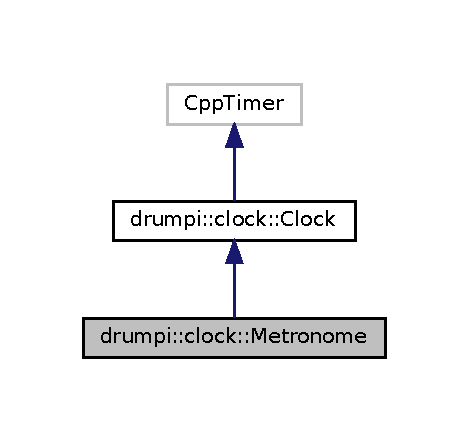
\includegraphics[width=210pt]{classdrumpi_1_1clock_1_1Metronome__coll__graph}
\end{center}
\end{figure}
\subsection*{Public Member Functions}
\begin{DoxyCompactItemize}
\item 
\hyperlink{classdrumpi_1_1clock_1_1Metronome_acc6e0b5140c79326682ec62eb879bf37}{Metronome} ()
\item 
void \hyperlink{classdrumpi_1_1clock_1_1Metronome_a831ff1dbeabee49fb64e468f4ecddaf0}{set\+Rate\+B\+PM} (int \hyperlink{classdrumpi_1_1clock_1_1Metronome_a5319099afdc9537cc8472233e5fbb0cc}{bpm})
\item 
int \hyperlink{classdrumpi_1_1clock_1_1Metronome_acd480d4bfe6d10a1990f9cac7578f071}{get\+Rate\+B\+PM} ()
\end{DoxyCompactItemize}
\subsection*{Private Attributes}
\begin{DoxyCompactItemize}
\item 
int \hyperlink{classdrumpi_1_1clock_1_1Metronome_a5319099afdc9537cc8472233e5fbb0cc}{bpm}
\end{DoxyCompactItemize}
\subsection*{Additional Inherited Members}


\subsection{Detailed Description}
\hyperlink{classdrumpi_1_1clock_1_1Metronome}{Metronome} class, similar to \hyperlink{classdrumpi_1_1clock_1_1Clock}{Clock} but can operate in B\+PM. To use, create a class that inherits from this and override the \hyperlink{classdrumpi_1_1clock_1_1Clock_ade9259c06e6b90bbd92e155a2506d3a1}{tick} method to set the functionality. 

\subsection{Constructor \& Destructor Documentation}
\mbox{\Hypertarget{classdrumpi_1_1clock_1_1Metronome_acc6e0b5140c79326682ec62eb879bf37}\label{classdrumpi_1_1clock_1_1Metronome_acc6e0b5140c79326682ec62eb879bf37}} 
\index{drumpi\+::clock\+::\+Metronome@{drumpi\+::clock\+::\+Metronome}!Metronome@{Metronome}}
\index{Metronome@{Metronome}!drumpi\+::clock\+::\+Metronome@{drumpi\+::clock\+::\+Metronome}}
\subsubsection{\texorpdfstring{Metronome()}{Metronome()}}
{\footnotesize\ttfamily Metronome\+::\+Metronome (\begin{DoxyParamCaption}{ }\end{DoxyParamCaption})}

Contructor. 

\subsection{Member Function Documentation}
\mbox{\Hypertarget{classdrumpi_1_1clock_1_1Metronome_acd480d4bfe6d10a1990f9cac7578f071}\label{classdrumpi_1_1clock_1_1Metronome_acd480d4bfe6d10a1990f9cac7578f071}} 
\index{drumpi\+::clock\+::\+Metronome@{drumpi\+::clock\+::\+Metronome}!get\+Rate\+B\+PM@{get\+Rate\+B\+PM}}
\index{get\+Rate\+B\+PM@{get\+Rate\+B\+PM}!drumpi\+::clock\+::\+Metronome@{drumpi\+::clock\+::\+Metronome}}
\subsubsection{\texorpdfstring{get\+Rate\+B\+P\+M()}{getRateBPM()}}
{\footnotesize\ttfamily int Metronome\+::get\+Rate\+B\+PM (\begin{DoxyParamCaption}{ }\end{DoxyParamCaption})}

Returns the clock rate in B\+PM. \begin{DoxyReturn}{Returns}
clock rate in B\+PM. 
\end{DoxyReturn}
\mbox{\Hypertarget{classdrumpi_1_1clock_1_1Metronome_a831ff1dbeabee49fb64e468f4ecddaf0}\label{classdrumpi_1_1clock_1_1Metronome_a831ff1dbeabee49fb64e468f4ecddaf0}} 
\index{drumpi\+::clock\+::\+Metronome@{drumpi\+::clock\+::\+Metronome}!set\+Rate\+B\+PM@{set\+Rate\+B\+PM}}
\index{set\+Rate\+B\+PM@{set\+Rate\+B\+PM}!drumpi\+::clock\+::\+Metronome@{drumpi\+::clock\+::\+Metronome}}
\subsubsection{\texorpdfstring{set\+Rate\+B\+P\+M()}{setRateBPM()}}
{\footnotesize\ttfamily void Metronome\+::set\+Rate\+B\+PM (\begin{DoxyParamCaption}\item[{int}]{bpm }\end{DoxyParamCaption})}

Sets the clock rate in B\+PM. The change takes effect on the next \hyperlink{classdrumpi_1_1clock_1_1Clock_ade9259c06e6b90bbd92e155a2506d3a1}{tick}, or can be forced by calling \hyperlink{classdrumpi_1_1clock_1_1Clock_a0b77c3e7f33eb7ae0f018e469d96a250}{stop} and then \hyperlink{classdrumpi_1_1clock_1_1Clock_a8a050959dcff11c85d695989e9099a8c}{start}. 
\begin{DoxyParams}{Parameters}
{\em bpm} & desired clocking rate in B\+PM. \\
\hline
\end{DoxyParams}


\subsection{Member Data Documentation}
\mbox{\Hypertarget{classdrumpi_1_1clock_1_1Metronome_a5319099afdc9537cc8472233e5fbb0cc}\label{classdrumpi_1_1clock_1_1Metronome_a5319099afdc9537cc8472233e5fbb0cc}} 
\index{drumpi\+::clock\+::\+Metronome@{drumpi\+::clock\+::\+Metronome}!bpm@{bpm}}
\index{bpm@{bpm}!drumpi\+::clock\+::\+Metronome@{drumpi\+::clock\+::\+Metronome}}
\subsubsection{\texorpdfstring{bpm}{bpm}}
{\footnotesize\ttfamily int drumpi\+::clock\+::\+Metronome\+::bpm\hspace{0.3cm}{\ttfamily [private]}}

\hyperlink{classdrumpi_1_1clock_1_1Clock}{Clock} rate in B\+PM. Stored to avoid quantisation issues from ms-\/to-\/\+B\+PM conversion. 

The documentation for this class was generated from the following files\+:\begin{DoxyCompactItemize}
\item 
src/clock.\+hpp\item 
src/clock.\+cpp\end{DoxyCompactItemize}

\hypertarget{classdrumpi_1_1PerformanceMode}{}\section{drumpi\+:\+:Performance\+Mode Class Reference}
\label{classdrumpi_1_1PerformanceMode}\index{drumpi\+::\+Performance\+Mode@{drumpi\+::\+Performance\+Mode}}


{\ttfamily \#include $<$application.\+hpp$>$}



Inheritance diagram for drumpi\+:\+:Performance\+Mode\+:
\nopagebreak
\begin{figure}[H]
\begin{center}
\leavevmode
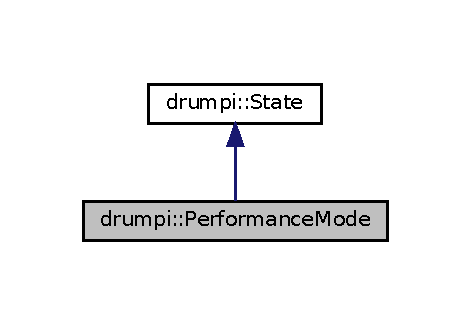
\includegraphics[width=211pt]{classdrumpi_1_1PerformanceMode__inherit__graph}
\end{center}
\end{figure}


Collaboration diagram for drumpi\+:\+:Performance\+Mode\+:
\nopagebreak
\begin{figure}[H]
\begin{center}
\leavevmode
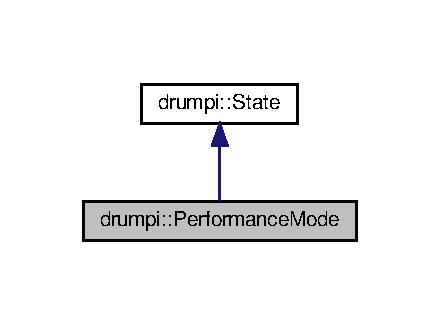
\includegraphics[width=211pt]{classdrumpi_1_1PerformanceMode__coll__graph}
\end{center}
\end{figure}
\subsection*{Public Member Functions}
\begin{DoxyCompactItemize}
\item 
\hyperlink{classdrumpi_1_1PerformanceMode_ae6b54e1ab335d25f6ad1aa52ea89e4df}{Performance\+Mode} ()
\item 
bool \hyperlink{classdrumpi_1_1PerformanceMode_a37c7c2eed9185a2211e389eebfd60262}{interpret\+Key\+Press} (\hyperlink{classdrumpi_1_1ApplicationCallback}{Application\+Callback} $\ast$appc, int key) override
\begin{DoxyCompactList}\small\item\em Performs an action depending on the key pressed. \end{DoxyCompactList}\item 
void \hyperlink{classdrumpi_1_1PerformanceMode_afc7bfd820bb21e4003ffe9ef189fa290}{update\+Display} (\hyperlink{classdrumpi_1_1ApplicationCallback}{Application\+Callback} $\ast$appc) override
\end{DoxyCompactItemize}
\subsection*{Additional Inherited Members}


\subsection{Detailed Description}
Performance mode state. 

\subsection{Constructor \& Destructor Documentation}
\mbox{\Hypertarget{classdrumpi_1_1PerformanceMode_ae6b54e1ab335d25f6ad1aa52ea89e4df}\label{classdrumpi_1_1PerformanceMode_ae6b54e1ab335d25f6ad1aa52ea89e4df}} 
\index{drumpi\+::\+Performance\+Mode@{drumpi\+::\+Performance\+Mode}!Performance\+Mode@{Performance\+Mode}}
\index{Performance\+Mode@{Performance\+Mode}!drumpi\+::\+Performance\+Mode@{drumpi\+::\+Performance\+Mode}}
\subsubsection{\texorpdfstring{Performance\+Mode()}{PerformanceMode()}}
{\footnotesize\ttfamily Performance\+Mode\+::\+Performance\+Mode (\begin{DoxyParamCaption}{ }\end{DoxyParamCaption})}

Constructor 

\subsection{Member Function Documentation}
\mbox{\Hypertarget{classdrumpi_1_1PerformanceMode_a37c7c2eed9185a2211e389eebfd60262}\label{classdrumpi_1_1PerformanceMode_a37c7c2eed9185a2211e389eebfd60262}} 
\index{drumpi\+::\+Performance\+Mode@{drumpi\+::\+Performance\+Mode}!interpret\+Key\+Press@{interpret\+Key\+Press}}
\index{interpret\+Key\+Press@{interpret\+Key\+Press}!drumpi\+::\+Performance\+Mode@{drumpi\+::\+Performance\+Mode}}
\subsubsection{\texorpdfstring{interpret\+Key\+Press()}{interpretKeyPress()}}
{\footnotesize\ttfamily bool Performance\+Mode\+::interpret\+Key\+Press (\begin{DoxyParamCaption}\item[{\hyperlink{classdrumpi_1_1ApplicationCallback}{Application\+Callback} $\ast$}]{appc,  }\item[{int}]{key }\end{DoxyParamCaption})\hspace{0.3cm}{\ttfamily [override]}, {\ttfamily [virtual]}}



Performs an action depending on the key pressed. 

This method is called by the \hyperlink{classdrumpi_1_1Application}{Application} when a keyboard event occurs and the application is in performance mode. 
\begin{DoxyParams}{Parameters}
{\em appc} & Callback to the main \hyperlink{classdrumpi_1_1Application}{Application}. \\
\hline
{\em key} & The keypress detected. \\
\hline
\end{DoxyParams}


Implements \hyperlink{classdrumpi_1_1State_aaa6205d85513b3f717c126e0717e1dbd}{drumpi\+::\+State}.

\mbox{\Hypertarget{classdrumpi_1_1PerformanceMode_afc7bfd820bb21e4003ffe9ef189fa290}\label{classdrumpi_1_1PerformanceMode_afc7bfd820bb21e4003ffe9ef189fa290}} 
\index{drumpi\+::\+Performance\+Mode@{drumpi\+::\+Performance\+Mode}!update\+Display@{update\+Display}}
\index{update\+Display@{update\+Display}!drumpi\+::\+Performance\+Mode@{drumpi\+::\+Performance\+Mode}}
\subsubsection{\texorpdfstring{update\+Display()}{updateDisplay()}}
{\footnotesize\ttfamily void Performance\+Mode\+::update\+Display (\begin{DoxyParamCaption}\item[{\hyperlink{classdrumpi_1_1ApplicationCallback}{Application\+Callback} $\ast$}]{appc }\end{DoxyParamCaption})\hspace{0.3cm}{\ttfamily [override]}, {\ttfamily [virtual]}}

Virtual function to be overridden by derived class. 

Implements \hyperlink{classdrumpi_1_1State_a400c5fc605ddec1e4fe18c361bf38ef2}{drumpi\+::\+State}.



The documentation for this class was generated from the following files\+:\begin{DoxyCompactItemize}
\item 
src/application.\+hpp\item 
src/application.\+cpp\end{DoxyCompactItemize}

\hypertarget{classdrumpi_1_1audio_1_1PlaybackEngine}{}\section{drumpi\+:\+:audio\+:\+:Playback\+Engine Class Reference}
\label{classdrumpi_1_1audio_1_1PlaybackEngine}\index{drumpi\+::audio\+::\+Playback\+Engine@{drumpi\+::audio\+::\+Playback\+Engine}}


{\ttfamily \#include $<$playback.\+hpp$>$}



Inheritance diagram for drumpi\+:\+:audio\+:\+:Playback\+Engine\+:
\nopagebreak
\begin{figure}[H]
\begin{center}
\leavevmode
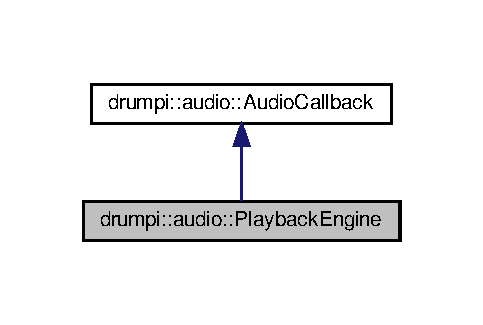
\includegraphics[width=232pt]{classdrumpi_1_1audio_1_1PlaybackEngine__inherit__graph}
\end{center}
\end{figure}


Collaboration diagram for drumpi\+:\+:audio\+:\+:Playback\+Engine\+:
\nopagebreak
\begin{figure}[H]
\begin{center}
\leavevmode
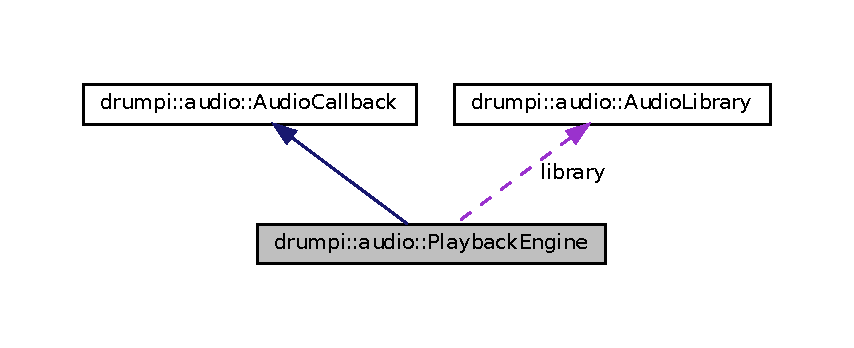
\includegraphics[width=350pt]{classdrumpi_1_1audio_1_1PlaybackEngine__coll__graph}
\end{center}
\end{figure}
\subsection*{Public Member Functions}
\begin{DoxyCompactItemize}
\item 
\hyperlink{classdrumpi_1_1audio_1_1PlaybackEngine_a19ac34713d360c934c987cac393152d2}{Playback\+Engine} ()
\item 
std\+::vector$<$ \hyperlink{namespacedrumpi_1_1audio_aca0bdc9164f87b72057e284442abab6e}{sample\+\_\+t} $>$ \hyperlink{classdrumpi_1_1audio_1_1PlaybackEngine_a16f4d8c36323b3b580475cd5fc4421c2}{get\+Samples} (int n\+Samples) override
\item 
void \hyperlink{classdrumpi_1_1audio_1_1PlaybackEngine_a0c089917f4288f1e8338df5ae11c6086}{trigger} (\hyperlink{namespacedrumpi_a3897274035c1b939a604438abe648b1b}{drum\+I\+D\+\_\+t} drum)
\item 
void \hyperlink{classdrumpi_1_1audio_1_1PlaybackEngine_a96c69e995f8c86a2fb5ac132a5bc2a22}{untrigger} (\hyperlink{namespacedrumpi_a3897274035c1b939a604438abe648b1b}{drum\+I\+D\+\_\+t} drum)
\item 
std\+::vector$<$ \hyperlink{namespacedrumpi_a3897274035c1b939a604438abe648b1b}{drum\+I\+D\+\_\+t} $>$ \hyperlink{classdrumpi_1_1audio_1_1PlaybackEngine_ac0400bef789e9d731bd8fef84da6f81e}{get\+Active} ()
\item 
void \hyperlink{classdrumpi_1_1audio_1_1PlaybackEngine_ac2010459b86f361199d812ad9123a948}{volume\+Up} (\hyperlink{namespacedrumpi_a3897274035c1b939a604438abe648b1b}{drum\+I\+D\+\_\+t} drum)
\item 
void \hyperlink{classdrumpi_1_1audio_1_1PlaybackEngine_a60538fdd91cf0891e0c5ba133e51dd98}{volume\+Up} ()
\item 
void \hyperlink{classdrumpi_1_1audio_1_1PlaybackEngine_aaef941772efa599c4782991676670145}{volume\+Down} (\hyperlink{namespacedrumpi_a3897274035c1b939a604438abe648b1b}{drum\+I\+D\+\_\+t} drum)
\item 
void \hyperlink{classdrumpi_1_1audio_1_1PlaybackEngine_ac11e4716ab1873f636ade9f762857427}{volume\+Down} ()
\item 
int \hyperlink{classdrumpi_1_1audio_1_1PlaybackEngine_aac50bd6f33b60955821231a57a9adc18}{get\+Volume} (\hyperlink{namespacedrumpi_a3897274035c1b939a604438abe648b1b}{drum\+I\+D\+\_\+t} drum)
\item 
int \hyperlink{classdrumpi_1_1audio_1_1PlaybackEngine_a3125be4c0e13e4a97c10d318e32a63b8}{get\+Volume} ()
\item 
\hyperlink{namespacedrumpi_1_1audio_a51bdf5757f414341f104d45e75e2bf63}{sample\+Source\+Status\+\_\+t} \hyperlink{classdrumpi_1_1audio_1_1PlaybackEngine_a3cf9336457c420b4d7a9f0e065743465}{load\+Bank} (int bank, \hyperlink{namespacedrumpi_1_1audio_a997f55e8a5b5348cf74dbedb7abe8a59}{sample\+Source\+Type\+\_\+t} type)
\item 
\hyperlink{namespacedrumpi_1_1audio_a51bdf5757f414341f104d45e75e2bf63}{sample\+Source\+Status\+\_\+t} \hyperlink{classdrumpi_1_1audio_1_1PlaybackEngine_a567803fa214f9c94abc4678e5013508c}{set\+Source} (\hyperlink{namespacedrumpi_a3897274035c1b939a604438abe648b1b}{drum\+I\+D\+\_\+t} drum, int bank, \hyperlink{namespacedrumpi_1_1audio_a997f55e8a5b5348cf74dbedb7abe8a59}{sample\+Source\+Type\+\_\+t} type)
\item 
\hyperlink{namespacedrumpi_1_1audio_a51bdf5757f414341f104d45e75e2bf63}{sample\+Source\+Status\+\_\+t} \hyperlink{classdrumpi_1_1audio_1_1PlaybackEngine_a2b2ce5172ee4c9b9cdf118b4c0972475}{get\+Source\+Status} (\hyperlink{namespacedrumpi_a3897274035c1b939a604438abe648b1b}{drum\+I\+D\+\_\+t} drum)
\item 
\hyperlink{namespacedrumpi_1_1audio_a997f55e8a5b5348cf74dbedb7abe8a59}{sample\+Source\+Type\+\_\+t} \hyperlink{classdrumpi_1_1audio_1_1PlaybackEngine_ab0c7e17c0a878563d98dcb316b9bf20f}{get\+Source\+Type} (\hyperlink{namespacedrumpi_a3897274035c1b939a604438abe648b1b}{drum\+I\+D\+\_\+t} drum)
\end{DoxyCompactItemize}
\subsection*{Private Attributes}
\begin{DoxyCompactItemize}
\item 
\hyperlink{classdrumpi_1_1audio_1_1AudioLibrary}{Audio\+Library} \hyperlink{classdrumpi_1_1audio_1_1PlaybackEngine_adb36e7fbdbf5155b9be32572fe2e74e7}{library}
\item 
std\+::vector$<$ \hyperlink{namespacedrumpi_1_1audio_aca0bdc9164f87b72057e284442abab6e}{sample\+\_\+t} $>$ \hyperlink{classdrumpi_1_1audio_1_1PlaybackEngine_af0c95ccde3dfb68503e775c50e65cd12}{buffer}
\item 
std\+::array$<$ std\+::unique\+\_\+ptr$<$ \hyperlink{classdrumpi_1_1audio_1_1SampleSource}{Sample\+Source} $>$, N\+U\+M\+\_\+\+D\+R\+U\+MS $>$ \hyperlink{classdrumpi_1_1audio_1_1PlaybackEngine_afe51646f62d3e7826f12f1fc4f90f57d}{sources}
\item 
std\+::array$<$ bool, N\+U\+M\+\_\+\+D\+R\+U\+MS $>$ \hyperlink{classdrumpi_1_1audio_1_1PlaybackEngine_a2ac98f97a163dfe1dd92da37722af803}{is\+Triggered}
\item 
int \hyperlink{classdrumpi_1_1audio_1_1PlaybackEngine_a3c706082f62476c77d9c95cee4828d12}{master\+Vol}
\item 
std\+::array$<$ int, N\+U\+M\+\_\+\+D\+R\+U\+MS $>$ \hyperlink{classdrumpi_1_1audio_1_1PlaybackEngine_af59868fe0bc057b1ae6bd00cbd795c56}{volumes}
\item 
std\+::array$<$ float, 101 $>$ \hyperlink{classdrumpi_1_1audio_1_1PlaybackEngine_ab546a7b63e007c69c7249f867768af0b}{volume\+Table}
\item 
const int \hyperlink{classdrumpi_1_1audio_1_1PlaybackEngine_a541e7697fd085bff60d86f3179f73f44}{master\+Vol\+Def} = 75
\item 
const int \hyperlink{classdrumpi_1_1audio_1_1PlaybackEngine_a701c2d92f46ae1f0d9654de2effd0145}{volume\+Def} = 75
\item 
const int \hyperlink{classdrumpi_1_1audio_1_1PlaybackEngine_a21a70337c53b12ff8e47662911bde068}{volume\+Step} = 5
\end{DoxyCompactItemize}


\subsection{Detailed Description}
Sample handling class. Manages audio clips for sending to output. An instance of this class is used as the callback class for the \hyperlink{classdrumpi_1_1audio_1_1JackClient}{Jack\+Client}. 

\subsection{Constructor \& Destructor Documentation}
\mbox{\Hypertarget{classdrumpi_1_1audio_1_1PlaybackEngine_a19ac34713d360c934c987cac393152d2}\label{classdrumpi_1_1audio_1_1PlaybackEngine_a19ac34713d360c934c987cac393152d2}} 
\index{drumpi\+::audio\+::\+Playback\+Engine@{drumpi\+::audio\+::\+Playback\+Engine}!Playback\+Engine@{Playback\+Engine}}
\index{Playback\+Engine@{Playback\+Engine}!drumpi\+::audio\+::\+Playback\+Engine@{drumpi\+::audio\+::\+Playback\+Engine}}
\subsubsection{\texorpdfstring{Playback\+Engine()}{PlaybackEngine()}}
{\footnotesize\ttfamily Playback\+Engine\+::\+Playback\+Engine (\begin{DoxyParamCaption}{ }\end{DoxyParamCaption})}

Constructor. 

\subsection{Member Function Documentation}
\mbox{\Hypertarget{classdrumpi_1_1audio_1_1PlaybackEngine_ac0400bef789e9d731bd8fef84da6f81e}\label{classdrumpi_1_1audio_1_1PlaybackEngine_ac0400bef789e9d731bd8fef84da6f81e}} 
\index{drumpi\+::audio\+::\+Playback\+Engine@{drumpi\+::audio\+::\+Playback\+Engine}!get\+Active@{get\+Active}}
\index{get\+Active@{get\+Active}!drumpi\+::audio\+::\+Playback\+Engine@{drumpi\+::audio\+::\+Playback\+Engine}}
\subsubsection{\texorpdfstring{get\+Active()}{getActive()}}
{\footnotesize\ttfamily std\+::vector$<$ \hyperlink{namespacedrumpi_a3897274035c1b939a604438abe648b1b}{drum\+I\+D\+\_\+t} $>$ Playback\+Engine\+::get\+Active (\begin{DoxyParamCaption}{ }\end{DoxyParamCaption})}

Returns a vector containing the \hyperlink{namespacedrumpi_a3897274035c1b939a604438abe648b1b}{drum\+I\+D\+\_\+t} of the currently active sources. \begin{DoxyReturn}{Returns}
vector of \hyperlink{namespacedrumpi_a3897274035c1b939a604438abe648b1b}{drum\+I\+D\+\_\+t} of the currently active sources. 
\end{DoxyReturn}
\mbox{\Hypertarget{classdrumpi_1_1audio_1_1PlaybackEngine_a16f4d8c36323b3b580475cd5fc4421c2}\label{classdrumpi_1_1audio_1_1PlaybackEngine_a16f4d8c36323b3b580475cd5fc4421c2}} 
\index{drumpi\+::audio\+::\+Playback\+Engine@{drumpi\+::audio\+::\+Playback\+Engine}!get\+Samples@{get\+Samples}}
\index{get\+Samples@{get\+Samples}!drumpi\+::audio\+::\+Playback\+Engine@{drumpi\+::audio\+::\+Playback\+Engine}}
\subsubsection{\texorpdfstring{get\+Samples()}{getSamples()}}
{\footnotesize\ttfamily std\+::vector$<$ \hyperlink{namespacedrumpi_1_1audio_aca0bdc9164f87b72057e284442abab6e}{sample\+\_\+t} $>$ Playback\+Engine\+::get\+Samples (\begin{DoxyParamCaption}\item[{int}]{n\+Samples }\end{DoxyParamCaption})\hspace{0.3cm}{\ttfamily [override]}, {\ttfamily [virtual]}}

Retrieves samples. 
\begin{DoxyParams}{Parameters}
{\em n\+Samples} & number of samples to return. \\
\hline
\end{DoxyParams}
\begin{DoxyReturn}{Returns}
a buffer of samples. 
\end{DoxyReturn}


Implements \hyperlink{classdrumpi_1_1audio_1_1AudioCallback_a9f53a830e6fd3d8eecf6f6ebb27314cd}{drumpi\+::audio\+::\+Audio\+Callback}.

\mbox{\Hypertarget{classdrumpi_1_1audio_1_1PlaybackEngine_a2b2ce5172ee4c9b9cdf118b4c0972475}\label{classdrumpi_1_1audio_1_1PlaybackEngine_a2b2ce5172ee4c9b9cdf118b4c0972475}} 
\index{drumpi\+::audio\+::\+Playback\+Engine@{drumpi\+::audio\+::\+Playback\+Engine}!get\+Source\+Status@{get\+Source\+Status}}
\index{get\+Source\+Status@{get\+Source\+Status}!drumpi\+::audio\+::\+Playback\+Engine@{drumpi\+::audio\+::\+Playback\+Engine}}
\subsubsection{\texorpdfstring{get\+Source\+Status()}{getSourceStatus()}}
{\footnotesize\ttfamily \hyperlink{namespacedrumpi_1_1audio_a51bdf5757f414341f104d45e75e2bf63}{sample\+Source\+Status\+\_\+t} Playback\+Engine\+::get\+Source\+Status (\begin{DoxyParamCaption}\item[{\hyperlink{namespacedrumpi_a3897274035c1b939a604438abe648b1b}{drum\+I\+D\+\_\+t}}]{drum }\end{DoxyParamCaption})}

Returns the source \hyperlink{namespacedrumpi_1_1audio_a51bdf5757f414341f104d45e75e2bf63}{sample\+Source\+Status\+\_\+t} of the given drum. \begin{DoxyReturn}{Returns}
source status. 
\end{DoxyReturn}
\mbox{\Hypertarget{classdrumpi_1_1audio_1_1PlaybackEngine_ab0c7e17c0a878563d98dcb316b9bf20f}\label{classdrumpi_1_1audio_1_1PlaybackEngine_ab0c7e17c0a878563d98dcb316b9bf20f}} 
\index{drumpi\+::audio\+::\+Playback\+Engine@{drumpi\+::audio\+::\+Playback\+Engine}!get\+Source\+Type@{get\+Source\+Type}}
\index{get\+Source\+Type@{get\+Source\+Type}!drumpi\+::audio\+::\+Playback\+Engine@{drumpi\+::audio\+::\+Playback\+Engine}}
\subsubsection{\texorpdfstring{get\+Source\+Type()}{getSourceType()}}
{\footnotesize\ttfamily \hyperlink{namespacedrumpi_1_1audio_a997f55e8a5b5348cf74dbedb7abe8a59}{sample\+Source\+Type\+\_\+t} Playback\+Engine\+::get\+Source\+Type (\begin{DoxyParamCaption}\item[{\hyperlink{namespacedrumpi_a3897274035c1b939a604438abe648b1b}{drum\+I\+D\+\_\+t}}]{drum }\end{DoxyParamCaption})}

Returns the source \hyperlink{namespacedrumpi_1_1audio_a997f55e8a5b5348cf74dbedb7abe8a59}{sample\+Source\+Type\+\_\+t} for the given drum. \begin{DoxyReturn}{Returns}
source type. 
\end{DoxyReturn}
\mbox{\Hypertarget{classdrumpi_1_1audio_1_1PlaybackEngine_aac50bd6f33b60955821231a57a9adc18}\label{classdrumpi_1_1audio_1_1PlaybackEngine_aac50bd6f33b60955821231a57a9adc18}} 
\index{drumpi\+::audio\+::\+Playback\+Engine@{drumpi\+::audio\+::\+Playback\+Engine}!get\+Volume@{get\+Volume}}
\index{get\+Volume@{get\+Volume}!drumpi\+::audio\+::\+Playback\+Engine@{drumpi\+::audio\+::\+Playback\+Engine}}
\subsubsection{\texorpdfstring{get\+Volume()}{getVolume()}\hspace{0.1cm}{\footnotesize\ttfamily [1/2]}}
{\footnotesize\ttfamily int Playback\+Engine\+::get\+Volume (\begin{DoxyParamCaption}\item[{\hyperlink{namespacedrumpi_a3897274035c1b939a604438abe648b1b}{drum\+I\+D\+\_\+t}}]{drum }\end{DoxyParamCaption})}

Returns the current volume of the passed drum as a percentage. 
\begin{DoxyParams}{Parameters}
{\em drum} & \hyperlink{namespacedrumpi_a3897274035c1b939a604438abe648b1b}{drum\+I\+D\+\_\+t} of the drum to query. \\
\hline
\end{DoxyParams}
\begin{DoxyReturn}{Returns}
current volume of drum. 
\end{DoxyReturn}
\mbox{\Hypertarget{classdrumpi_1_1audio_1_1PlaybackEngine_a3125be4c0e13e4a97c10d318e32a63b8}\label{classdrumpi_1_1audio_1_1PlaybackEngine_a3125be4c0e13e4a97c10d318e32a63b8}} 
\index{drumpi\+::audio\+::\+Playback\+Engine@{drumpi\+::audio\+::\+Playback\+Engine}!get\+Volume@{get\+Volume}}
\index{get\+Volume@{get\+Volume}!drumpi\+::audio\+::\+Playback\+Engine@{drumpi\+::audio\+::\+Playback\+Engine}}
\subsubsection{\texorpdfstring{get\+Volume()}{getVolume()}\hspace{0.1cm}{\footnotesize\ttfamily [2/2]}}
{\footnotesize\ttfamily int Playback\+Engine\+::get\+Volume (\begin{DoxyParamCaption}{ }\end{DoxyParamCaption})}

Returns the current master volume as a percentage. \begin{DoxyReturn}{Returns}
current master volume. 
\end{DoxyReturn}
\mbox{\Hypertarget{classdrumpi_1_1audio_1_1PlaybackEngine_a3cf9336457c420b4d7a9f0e065743465}\label{classdrumpi_1_1audio_1_1PlaybackEngine_a3cf9336457c420b4d7a9f0e065743465}} 
\index{drumpi\+::audio\+::\+Playback\+Engine@{drumpi\+::audio\+::\+Playback\+Engine}!load\+Bank@{load\+Bank}}
\index{load\+Bank@{load\+Bank}!drumpi\+::audio\+::\+Playback\+Engine@{drumpi\+::audio\+::\+Playback\+Engine}}
\subsubsection{\texorpdfstring{load\+Bank()}{loadBank()}}
{\footnotesize\ttfamily \hyperlink{namespacedrumpi_1_1audio_a51bdf5757f414341f104d45e75e2bf63}{sample\+Source\+Status\+\_\+t} Playback\+Engine\+::load\+Bank (\begin{DoxyParamCaption}\item[{int}]{bank,  }\item[{\hyperlink{namespacedrumpi_1_1audio_a997f55e8a5b5348cf74dbedb7abe8a59}{sample\+Source\+Type\+\_\+t}}]{type }\end{DoxyParamCaption})}

Loads a bank of drums of a homogenous \hyperlink{namespacedrumpi_1_1audio_a997f55e8a5b5348cf74dbedb7abe8a59}{sample\+Source\+Type\+\_\+t}. 
\begin{DoxyParams}{Parameters}
{\em bank} & ID of the bank of drums to load from. \\
\hline
{\em type} & \hyperlink{namespacedrumpi_1_1audio_a997f55e8a5b5348cf74dbedb7abe8a59}{sample\+Source\+Type\+\_\+t} of sources to load. \\
\hline
\end{DoxyParams}
\mbox{\Hypertarget{classdrumpi_1_1audio_1_1PlaybackEngine_a567803fa214f9c94abc4678e5013508c}\label{classdrumpi_1_1audio_1_1PlaybackEngine_a567803fa214f9c94abc4678e5013508c}} 
\index{drumpi\+::audio\+::\+Playback\+Engine@{drumpi\+::audio\+::\+Playback\+Engine}!set\+Source@{set\+Source}}
\index{set\+Source@{set\+Source}!drumpi\+::audio\+::\+Playback\+Engine@{drumpi\+::audio\+::\+Playback\+Engine}}
\subsubsection{\texorpdfstring{set\+Source()}{setSource()}}
{\footnotesize\ttfamily \hyperlink{namespacedrumpi_1_1audio_a51bdf5757f414341f104d45e75e2bf63}{sample\+Source\+Status\+\_\+t} Playback\+Engine\+::set\+Source (\begin{DoxyParamCaption}\item[{\hyperlink{namespacedrumpi_a3897274035c1b939a604438abe648b1b}{drum\+I\+D\+\_\+t}}]{drum,  }\item[{int}]{bank,  }\item[{\hyperlink{namespacedrumpi_1_1audio_a997f55e8a5b5348cf74dbedb7abe8a59}{sample\+Source\+Type\+\_\+t}}]{type }\end{DoxyParamCaption})}

Sets the source for the specified drum. 
\begin{DoxyParams}{Parameters}
{\em drum} & \hyperlink{namespacedrumpi_a3897274035c1b939a604438abe648b1b}{drum\+I\+D\+\_\+t} of the drum to set the type for. \\
\hline
{\em bank} & ID of the bank of drums to load from. \\
\hline
{\em type} & \hyperlink{namespacedrumpi_1_1audio_a997f55e8a5b5348cf74dbedb7abe8a59}{sample\+Source\+Type\+\_\+t} of source to load. \\
\hline
\end{DoxyParams}
\mbox{\Hypertarget{classdrumpi_1_1audio_1_1PlaybackEngine_a0c089917f4288f1e8338df5ae11c6086}\label{classdrumpi_1_1audio_1_1PlaybackEngine_a0c089917f4288f1e8338df5ae11c6086}} 
\index{drumpi\+::audio\+::\+Playback\+Engine@{drumpi\+::audio\+::\+Playback\+Engine}!trigger@{trigger}}
\index{trigger@{trigger}!drumpi\+::audio\+::\+Playback\+Engine@{drumpi\+::audio\+::\+Playback\+Engine}}
\subsubsection{\texorpdfstring{trigger()}{trigger()}}
{\footnotesize\ttfamily void Playback\+Engine\+::trigger (\begin{DoxyParamCaption}\item[{\hyperlink{namespacedrumpi_a3897274035c1b939a604438abe648b1b}{drum\+I\+D\+\_\+t}}]{drum }\end{DoxyParamCaption})}

Adds the specified drum to the output stream. 
\begin{DoxyParams}{Parameters}
{\em drum} & \hyperlink{namespacedrumpi_a3897274035c1b939a604438abe648b1b}{drum\+I\+D\+\_\+t} of the drum to add. \\
\hline
\end{DoxyParams}
\mbox{\Hypertarget{classdrumpi_1_1audio_1_1PlaybackEngine_a96c69e995f8c86a2fb5ac132a5bc2a22}\label{classdrumpi_1_1audio_1_1PlaybackEngine_a96c69e995f8c86a2fb5ac132a5bc2a22}} 
\index{drumpi\+::audio\+::\+Playback\+Engine@{drumpi\+::audio\+::\+Playback\+Engine}!untrigger@{untrigger}}
\index{untrigger@{untrigger}!drumpi\+::audio\+::\+Playback\+Engine@{drumpi\+::audio\+::\+Playback\+Engine}}
\subsubsection{\texorpdfstring{untrigger()}{untrigger()}}
{\footnotesize\ttfamily void Playback\+Engine\+::untrigger (\begin{DoxyParamCaption}\item[{\hyperlink{namespacedrumpi_a3897274035c1b939a604438abe648b1b}{drum\+I\+D\+\_\+t}}]{drum }\end{DoxyParamCaption})}

Removes the specified drum sample from the output. 
\begin{DoxyParams}{Parameters}
{\em drum} & \hyperlink{namespacedrumpi_a3897274035c1b939a604438abe648b1b}{drum\+I\+D\+\_\+t} of the drum to remove. \\
\hline
\end{DoxyParams}
\mbox{\Hypertarget{classdrumpi_1_1audio_1_1PlaybackEngine_aaef941772efa599c4782991676670145}\label{classdrumpi_1_1audio_1_1PlaybackEngine_aaef941772efa599c4782991676670145}} 
\index{drumpi\+::audio\+::\+Playback\+Engine@{drumpi\+::audio\+::\+Playback\+Engine}!volume\+Down@{volume\+Down}}
\index{volume\+Down@{volume\+Down}!drumpi\+::audio\+::\+Playback\+Engine@{drumpi\+::audio\+::\+Playback\+Engine}}
\subsubsection{\texorpdfstring{volume\+Down()}{volumeDown()}\hspace{0.1cm}{\footnotesize\ttfamily [1/2]}}
{\footnotesize\ttfamily void Playback\+Engine\+::volume\+Down (\begin{DoxyParamCaption}\item[{\hyperlink{namespacedrumpi_a3897274035c1b939a604438abe648b1b}{drum\+I\+D\+\_\+t}}]{drum }\end{DoxyParamCaption})}

Decrements the playback volume for the passed drum. 
\begin{DoxyParams}{Parameters}
{\em drum} & \hyperlink{namespacedrumpi_a3897274035c1b939a604438abe648b1b}{drum\+I\+D\+\_\+t} of the drum to be affected. \\
\hline
\end{DoxyParams}
\mbox{\Hypertarget{classdrumpi_1_1audio_1_1PlaybackEngine_ac11e4716ab1873f636ade9f762857427}\label{classdrumpi_1_1audio_1_1PlaybackEngine_ac11e4716ab1873f636ade9f762857427}} 
\index{drumpi\+::audio\+::\+Playback\+Engine@{drumpi\+::audio\+::\+Playback\+Engine}!volume\+Down@{volume\+Down}}
\index{volume\+Down@{volume\+Down}!drumpi\+::audio\+::\+Playback\+Engine@{drumpi\+::audio\+::\+Playback\+Engine}}
\subsubsection{\texorpdfstring{volume\+Down()}{volumeDown()}\hspace{0.1cm}{\footnotesize\ttfamily [2/2]}}
{\footnotesize\ttfamily void Playback\+Engine\+::volume\+Down (\begin{DoxyParamCaption}{ }\end{DoxyParamCaption})}

Decrements the master output volume. \mbox{\Hypertarget{classdrumpi_1_1audio_1_1PlaybackEngine_ac2010459b86f361199d812ad9123a948}\label{classdrumpi_1_1audio_1_1PlaybackEngine_ac2010459b86f361199d812ad9123a948}} 
\index{drumpi\+::audio\+::\+Playback\+Engine@{drumpi\+::audio\+::\+Playback\+Engine}!volume\+Up@{volume\+Up}}
\index{volume\+Up@{volume\+Up}!drumpi\+::audio\+::\+Playback\+Engine@{drumpi\+::audio\+::\+Playback\+Engine}}
\subsubsection{\texorpdfstring{volume\+Up()}{volumeUp()}\hspace{0.1cm}{\footnotesize\ttfamily [1/2]}}
{\footnotesize\ttfamily void Playback\+Engine\+::volume\+Up (\begin{DoxyParamCaption}\item[{\hyperlink{namespacedrumpi_a3897274035c1b939a604438abe648b1b}{drum\+I\+D\+\_\+t}}]{drum }\end{DoxyParamCaption})}

Increments the playback volume for the passed drum. 
\begin{DoxyParams}{Parameters}
{\em drum} & \hyperlink{namespacedrumpi_a3897274035c1b939a604438abe648b1b}{drum\+I\+D\+\_\+t} of the drum to be affected. \\
\hline
\end{DoxyParams}
\mbox{\Hypertarget{classdrumpi_1_1audio_1_1PlaybackEngine_a60538fdd91cf0891e0c5ba133e51dd98}\label{classdrumpi_1_1audio_1_1PlaybackEngine_a60538fdd91cf0891e0c5ba133e51dd98}} 
\index{drumpi\+::audio\+::\+Playback\+Engine@{drumpi\+::audio\+::\+Playback\+Engine}!volume\+Up@{volume\+Up}}
\index{volume\+Up@{volume\+Up}!drumpi\+::audio\+::\+Playback\+Engine@{drumpi\+::audio\+::\+Playback\+Engine}}
\subsubsection{\texorpdfstring{volume\+Up()}{volumeUp()}\hspace{0.1cm}{\footnotesize\ttfamily [2/2]}}
{\footnotesize\ttfamily void Playback\+Engine\+::volume\+Up (\begin{DoxyParamCaption}{ }\end{DoxyParamCaption})}

Increments the master output volume. 

\subsection{Member Data Documentation}
\mbox{\Hypertarget{classdrumpi_1_1audio_1_1PlaybackEngine_af0c95ccde3dfb68503e775c50e65cd12}\label{classdrumpi_1_1audio_1_1PlaybackEngine_af0c95ccde3dfb68503e775c50e65cd12}} 
\index{drumpi\+::audio\+::\+Playback\+Engine@{drumpi\+::audio\+::\+Playback\+Engine}!buffer@{buffer}}
\index{buffer@{buffer}!drumpi\+::audio\+::\+Playback\+Engine@{drumpi\+::audio\+::\+Playback\+Engine}}
\subsubsection{\texorpdfstring{buffer}{buffer}}
{\footnotesize\ttfamily std\+::vector$<$\hyperlink{namespacedrumpi_1_1audio_aca0bdc9164f87b72057e284442abab6e}{sample\+\_\+t}$>$ drumpi\+::audio\+::\+Playback\+Engine\+::buffer\hspace{0.3cm}{\ttfamily [private]}}

Buffer of samples to allow rapid transfer to Jack. \mbox{\Hypertarget{classdrumpi_1_1audio_1_1PlaybackEngine_a2ac98f97a163dfe1dd92da37722af803}\label{classdrumpi_1_1audio_1_1PlaybackEngine_a2ac98f97a163dfe1dd92da37722af803}} 
\index{drumpi\+::audio\+::\+Playback\+Engine@{drumpi\+::audio\+::\+Playback\+Engine}!is\+Triggered@{is\+Triggered}}
\index{is\+Triggered@{is\+Triggered}!drumpi\+::audio\+::\+Playback\+Engine@{drumpi\+::audio\+::\+Playback\+Engine}}
\subsubsection{\texorpdfstring{is\+Triggered}{isTriggered}}
{\footnotesize\ttfamily std\+::array$<$bool, N\+U\+M\+\_\+\+D\+R\+U\+MS$>$ drumpi\+::audio\+::\+Playback\+Engine\+::is\+Triggered\hspace{0.3cm}{\ttfamily [private]}}

Switches to store whether each source is being played. \mbox{\Hypertarget{classdrumpi_1_1audio_1_1PlaybackEngine_adb36e7fbdbf5155b9be32572fe2e74e7}\label{classdrumpi_1_1audio_1_1PlaybackEngine_adb36e7fbdbf5155b9be32572fe2e74e7}} 
\index{drumpi\+::audio\+::\+Playback\+Engine@{drumpi\+::audio\+::\+Playback\+Engine}!library@{library}}
\index{library@{library}!drumpi\+::audio\+::\+Playback\+Engine@{drumpi\+::audio\+::\+Playback\+Engine}}
\subsubsection{\texorpdfstring{library}{library}}
{\footnotesize\ttfamily \hyperlink{classdrumpi_1_1audio_1_1AudioLibrary}{Audio\+Library} drumpi\+::audio\+::\+Playback\+Engine\+::library\hspace{0.3cm}{\ttfamily [private]}}

Library manager for the audio sources. \mbox{\Hypertarget{classdrumpi_1_1audio_1_1PlaybackEngine_a3c706082f62476c77d9c95cee4828d12}\label{classdrumpi_1_1audio_1_1PlaybackEngine_a3c706082f62476c77d9c95cee4828d12}} 
\index{drumpi\+::audio\+::\+Playback\+Engine@{drumpi\+::audio\+::\+Playback\+Engine}!master\+Vol@{master\+Vol}}
\index{master\+Vol@{master\+Vol}!drumpi\+::audio\+::\+Playback\+Engine@{drumpi\+::audio\+::\+Playback\+Engine}}
\subsubsection{\texorpdfstring{master\+Vol}{masterVol}}
{\footnotesize\ttfamily int drumpi\+::audio\+::\+Playback\+Engine\+::master\+Vol\hspace{0.3cm}{\ttfamily [private]}}

Current master volume as a percentage. \mbox{\Hypertarget{classdrumpi_1_1audio_1_1PlaybackEngine_a541e7697fd085bff60d86f3179f73f44}\label{classdrumpi_1_1audio_1_1PlaybackEngine_a541e7697fd085bff60d86f3179f73f44}} 
\index{drumpi\+::audio\+::\+Playback\+Engine@{drumpi\+::audio\+::\+Playback\+Engine}!master\+Vol\+Def@{master\+Vol\+Def}}
\index{master\+Vol\+Def@{master\+Vol\+Def}!drumpi\+::audio\+::\+Playback\+Engine@{drumpi\+::audio\+::\+Playback\+Engine}}
\subsubsection{\texorpdfstring{master\+Vol\+Def}{masterVolDef}}
{\footnotesize\ttfamily const int drumpi\+::audio\+::\+Playback\+Engine\+::master\+Vol\+Def = 75\hspace{0.3cm}{\ttfamily [private]}}

Default master volume. \mbox{\Hypertarget{classdrumpi_1_1audio_1_1PlaybackEngine_afe51646f62d3e7826f12f1fc4f90f57d}\label{classdrumpi_1_1audio_1_1PlaybackEngine_afe51646f62d3e7826f12f1fc4f90f57d}} 
\index{drumpi\+::audio\+::\+Playback\+Engine@{drumpi\+::audio\+::\+Playback\+Engine}!sources@{sources}}
\index{sources@{sources}!drumpi\+::audio\+::\+Playback\+Engine@{drumpi\+::audio\+::\+Playback\+Engine}}
\subsubsection{\texorpdfstring{sources}{sources}}
{\footnotesize\ttfamily std\+::array$<$std\+::unique\+\_\+ptr$<$\hyperlink{classdrumpi_1_1audio_1_1SampleSource}{Sample\+Source}$>$, N\+U\+M\+\_\+\+D\+R\+U\+MS$>$ drumpi\+::audio\+::\+Playback\+Engine\+::sources\hspace{0.3cm}{\ttfamily [private]}}

\hyperlink{classdrumpi_1_1audio_1_1SampleSource}{Sample\+Source} object pointers. \mbox{\Hypertarget{classdrumpi_1_1audio_1_1PlaybackEngine_a701c2d92f46ae1f0d9654de2effd0145}\label{classdrumpi_1_1audio_1_1PlaybackEngine_a701c2d92f46ae1f0d9654de2effd0145}} 
\index{drumpi\+::audio\+::\+Playback\+Engine@{drumpi\+::audio\+::\+Playback\+Engine}!volume\+Def@{volume\+Def}}
\index{volume\+Def@{volume\+Def}!drumpi\+::audio\+::\+Playback\+Engine@{drumpi\+::audio\+::\+Playback\+Engine}}
\subsubsection{\texorpdfstring{volume\+Def}{volumeDef}}
{\footnotesize\ttfamily const int drumpi\+::audio\+::\+Playback\+Engine\+::volume\+Def = 75\hspace{0.3cm}{\ttfamily [private]}}

Default drum volume. \mbox{\Hypertarget{classdrumpi_1_1audio_1_1PlaybackEngine_af59868fe0bc057b1ae6bd00cbd795c56}\label{classdrumpi_1_1audio_1_1PlaybackEngine_af59868fe0bc057b1ae6bd00cbd795c56}} 
\index{drumpi\+::audio\+::\+Playback\+Engine@{drumpi\+::audio\+::\+Playback\+Engine}!volumes@{volumes}}
\index{volumes@{volumes}!drumpi\+::audio\+::\+Playback\+Engine@{drumpi\+::audio\+::\+Playback\+Engine}}
\subsubsection{\texorpdfstring{volumes}{volumes}}
{\footnotesize\ttfamily std\+::array$<$int, N\+U\+M\+\_\+\+D\+R\+U\+MS$>$ drumpi\+::audio\+::\+Playback\+Engine\+::volumes\hspace{0.3cm}{\ttfamily [private]}}

Current drum volumes as percentages. \mbox{\Hypertarget{classdrumpi_1_1audio_1_1PlaybackEngine_a21a70337c53b12ff8e47662911bde068}\label{classdrumpi_1_1audio_1_1PlaybackEngine_a21a70337c53b12ff8e47662911bde068}} 
\index{drumpi\+::audio\+::\+Playback\+Engine@{drumpi\+::audio\+::\+Playback\+Engine}!volume\+Step@{volume\+Step}}
\index{volume\+Step@{volume\+Step}!drumpi\+::audio\+::\+Playback\+Engine@{drumpi\+::audio\+::\+Playback\+Engine}}
\subsubsection{\texorpdfstring{volume\+Step}{volumeStep}}
{\footnotesize\ttfamily const int drumpi\+::audio\+::\+Playback\+Engine\+::volume\+Step = 5\hspace{0.3cm}{\ttfamily [private]}}

Step size for volume increments and decrements. \mbox{\Hypertarget{classdrumpi_1_1audio_1_1PlaybackEngine_ab546a7b63e007c69c7249f867768af0b}\label{classdrumpi_1_1audio_1_1PlaybackEngine_ab546a7b63e007c69c7249f867768af0b}} 
\index{drumpi\+::audio\+::\+Playback\+Engine@{drumpi\+::audio\+::\+Playback\+Engine}!volume\+Table@{volume\+Table}}
\index{volume\+Table@{volume\+Table}!drumpi\+::audio\+::\+Playback\+Engine@{drumpi\+::audio\+::\+Playback\+Engine}}
\subsubsection{\texorpdfstring{volume\+Table}{volumeTable}}
{\footnotesize\ttfamily std\+::array$<$float, 101$>$ drumpi\+::audio\+::\+Playback\+Engine\+::volume\+Table\hspace{0.3cm}{\ttfamily [private]}}

Lookup table for exponential volume control. Indexed as a percentage. 

The documentation for this class was generated from the following files\+:\begin{DoxyCompactItemize}
\item 
src/playback.\+hpp\item 
src/playback.\+cpp\end{DoxyCompactItemize}

\hypertarget{classdrumpi_1_1audio_1_1SampleSource}{}\section{drumpi\+:\+:audio\+:\+:Sample\+Source Class Reference}
\label{classdrumpi_1_1audio_1_1SampleSource}\index{drumpi\+::audio\+::\+Sample\+Source@{drumpi\+::audio\+::\+Sample\+Source}}


{\ttfamily \#include $<$sample\+Source.\+hpp$>$}



Inheritance diagram for drumpi\+:\+:audio\+:\+:Sample\+Source\+:
\nopagebreak
\begin{figure}[H]
\begin{center}
\leavevmode
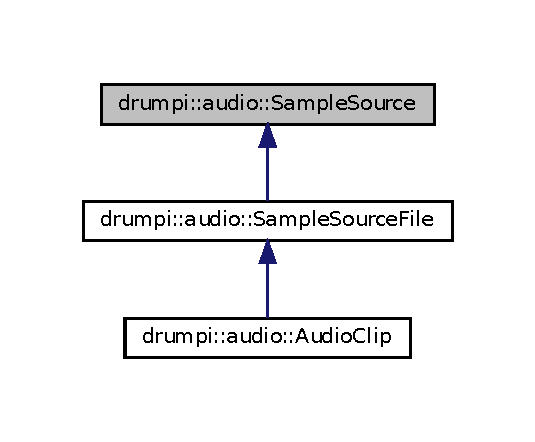
\includegraphics[width=241pt]{classdrumpi_1_1audio_1_1SampleSource__inherit__graph}
\end{center}
\end{figure}
\subsection*{Public Member Functions}
\begin{DoxyCompactItemize}
\item 
\hyperlink{classdrumpi_1_1audio_1_1SampleSource_a8c83ab0aa33861c5f88783b3a818ffba}{Sample\+Source} ()
\item 
virtual std\+::vector$<$ \hyperlink{namespacedrumpi_1_1audio_aca0bdc9164f87b72057e284442abab6e}{sample\+\_\+t} $>$ \hyperlink{classdrumpi_1_1audio_1_1SampleSource_ab3f12884325b818ebe088dec5daa15cd}{get\+Samples} (int n\+Samples)=0
\item 
virtual void \hyperlink{classdrumpi_1_1audio_1_1SampleSource_aa7b214c99ee55ceac758fdef44b0cd6d}{reset} ()=0
\item 
virtual void \hyperlink{classdrumpi_1_1audio_1_1SampleSource_aff9beb7031bc5af424dccc525be5e9d3}{update\+Status} ()=0
\item 
\hyperlink{namespacedrumpi_1_1audio_a51bdf5757f414341f104d45e75e2bf63}{sample\+Source\+Status\+\_\+t} \hyperlink{classdrumpi_1_1audio_1_1SampleSource_a9fea9c824e15d891cbacbf4c5187c2aa}{get\+Status} ()
\item 
\hyperlink{namespacedrumpi_1_1audio_a997f55e8a5b5348cf74dbedb7abe8a59}{sample\+Source\+Type\+\_\+t} \hyperlink{classdrumpi_1_1audio_1_1SampleSource_a83b000d9fe8335788f4ba876b13b4b66}{get\+Type} ()
\end{DoxyCompactItemize}
\subsection*{Protected Attributes}
\begin{DoxyCompactItemize}
\item 
\hyperlink{namespacedrumpi_1_1audio_a51bdf5757f414341f104d45e75e2bf63}{sample\+Source\+Status\+\_\+t} \hyperlink{classdrumpi_1_1audio_1_1SampleSource_a0278ea1fe44e5c1c643d6c8549302f19}{status}
\item 
\hyperlink{namespacedrumpi_1_1audio_a997f55e8a5b5348cf74dbedb7abe8a59}{sample\+Source\+Type\+\_\+t} \hyperlink{classdrumpi_1_1audio_1_1SampleSource_af3411ed42fcc880fb0a69d2dd80aac18}{type}
\end{DoxyCompactItemize}


\subsection{Detailed Description}
Abstract class for sample retieval. 

\subsection{Constructor \& Destructor Documentation}
\mbox{\Hypertarget{classdrumpi_1_1audio_1_1SampleSource_a8c83ab0aa33861c5f88783b3a818ffba}\label{classdrumpi_1_1audio_1_1SampleSource_a8c83ab0aa33861c5f88783b3a818ffba}} 
\index{drumpi\+::audio\+::\+Sample\+Source@{drumpi\+::audio\+::\+Sample\+Source}!Sample\+Source@{Sample\+Source}}
\index{Sample\+Source@{Sample\+Source}!drumpi\+::audio\+::\+Sample\+Source@{drumpi\+::audio\+::\+Sample\+Source}}
\subsubsection{\texorpdfstring{Sample\+Source()}{SampleSource()}}
{\footnotesize\ttfamily Sample\+Source\+::\+Sample\+Source (\begin{DoxyParamCaption}{ }\end{DoxyParamCaption})}

Constructor. 

\subsection{Member Function Documentation}
\mbox{\Hypertarget{classdrumpi_1_1audio_1_1SampleSource_ab3f12884325b818ebe088dec5daa15cd}\label{classdrumpi_1_1audio_1_1SampleSource_ab3f12884325b818ebe088dec5daa15cd}} 
\index{drumpi\+::audio\+::\+Sample\+Source@{drumpi\+::audio\+::\+Sample\+Source}!get\+Samples@{get\+Samples}}
\index{get\+Samples@{get\+Samples}!drumpi\+::audio\+::\+Sample\+Source@{drumpi\+::audio\+::\+Sample\+Source}}
\subsubsection{\texorpdfstring{get\+Samples()}{getSamples()}}
{\footnotesize\ttfamily virtual std\+::vector$<$\hyperlink{namespacedrumpi_1_1audio_aca0bdc9164f87b72057e284442abab6e}{sample\+\_\+t}$>$ drumpi\+::audio\+::\+Sample\+Source\+::get\+Samples (\begin{DoxyParamCaption}\item[{int}]{n\+Samples }\end{DoxyParamCaption})\hspace{0.3cm}{\ttfamily [pure virtual]}}

Returns a buffer of samples. 
\begin{DoxyParams}{Parameters}
{\em n\+Samples} & number of samples to be returned. \\
\hline
\end{DoxyParams}
\begin{DoxyReturn}{Returns}
a sample buffer of length n\+Samples. 
\end{DoxyReturn}


Implemented in \hyperlink{classdrumpi_1_1audio_1_1AudioClip_aad8e2b4282047c0fb884d4f93210c83b}{drumpi\+::audio\+::\+Audio\+Clip}.

\mbox{\Hypertarget{classdrumpi_1_1audio_1_1SampleSource_a9fea9c824e15d891cbacbf4c5187c2aa}\label{classdrumpi_1_1audio_1_1SampleSource_a9fea9c824e15d891cbacbf4c5187c2aa}} 
\index{drumpi\+::audio\+::\+Sample\+Source@{drumpi\+::audio\+::\+Sample\+Source}!get\+Status@{get\+Status}}
\index{get\+Status@{get\+Status}!drumpi\+::audio\+::\+Sample\+Source@{drumpi\+::audio\+::\+Sample\+Source}}
\subsubsection{\texorpdfstring{get\+Status()}{getStatus()}}
{\footnotesize\ttfamily \hyperlink{namespacedrumpi_1_1audio_a51bdf5757f414341f104d45e75e2bf63}{sample\+Source\+Status\+\_\+t} Sample\+Source\+::get\+Status (\begin{DoxyParamCaption}{ }\end{DoxyParamCaption})}

Returns the status of the source. \begin{DoxyReturn}{Returns}
status code of source. 
\end{DoxyReturn}
\mbox{\Hypertarget{classdrumpi_1_1audio_1_1SampleSource_a83b000d9fe8335788f4ba876b13b4b66}\label{classdrumpi_1_1audio_1_1SampleSource_a83b000d9fe8335788f4ba876b13b4b66}} 
\index{drumpi\+::audio\+::\+Sample\+Source@{drumpi\+::audio\+::\+Sample\+Source}!get\+Type@{get\+Type}}
\index{get\+Type@{get\+Type}!drumpi\+::audio\+::\+Sample\+Source@{drumpi\+::audio\+::\+Sample\+Source}}
\subsubsection{\texorpdfstring{get\+Type()}{getType()}}
{\footnotesize\ttfamily \hyperlink{namespacedrumpi_1_1audio_a997f55e8a5b5348cf74dbedb7abe8a59}{sample\+Source\+Type\+\_\+t} Sample\+Source\+::get\+Type (\begin{DoxyParamCaption}{ }\end{DoxyParamCaption})}

Returns the type of source represented by the object. \begin{DoxyReturn}{Returns}
type code of source 
\end{DoxyReturn}
\mbox{\Hypertarget{classdrumpi_1_1audio_1_1SampleSource_aa7b214c99ee55ceac758fdef44b0cd6d}\label{classdrumpi_1_1audio_1_1SampleSource_aa7b214c99ee55ceac758fdef44b0cd6d}} 
\index{drumpi\+::audio\+::\+Sample\+Source@{drumpi\+::audio\+::\+Sample\+Source}!reset@{reset}}
\index{reset@{reset}!drumpi\+::audio\+::\+Sample\+Source@{drumpi\+::audio\+::\+Sample\+Source}}
\subsubsection{\texorpdfstring{reset()}{reset()}}
{\footnotesize\ttfamily virtual void drumpi\+::audio\+::\+Sample\+Source\+::reset (\begin{DoxyParamCaption}{ }\end{DoxyParamCaption})\hspace{0.3cm}{\ttfamily [pure virtual]}}

Resets the source to initial conditions. 

Implemented in \hyperlink{classdrumpi_1_1audio_1_1AudioClip_ac870bf37050afae302754c4e4671d779}{drumpi\+::audio\+::\+Audio\+Clip}.

\mbox{\Hypertarget{classdrumpi_1_1audio_1_1SampleSource_aff9beb7031bc5af424dccc525be5e9d3}\label{classdrumpi_1_1audio_1_1SampleSource_aff9beb7031bc5af424dccc525be5e9d3}} 
\index{drumpi\+::audio\+::\+Sample\+Source@{drumpi\+::audio\+::\+Sample\+Source}!update\+Status@{update\+Status}}
\index{update\+Status@{update\+Status}!drumpi\+::audio\+::\+Sample\+Source@{drumpi\+::audio\+::\+Sample\+Source}}
\subsubsection{\texorpdfstring{update\+Status()}{updateStatus()}}
{\footnotesize\ttfamily virtual void drumpi\+::audio\+::\+Sample\+Source\+::update\+Status (\begin{DoxyParamCaption}{ }\end{DoxyParamCaption})\hspace{0.3cm}{\ttfamily [pure virtual]}}

Updates the status of the source. 

Implemented in \hyperlink{classdrumpi_1_1audio_1_1AudioClip_aeed08721b08d9443a769a99e717f5743}{drumpi\+::audio\+::\+Audio\+Clip}.



\subsection{Member Data Documentation}
\mbox{\Hypertarget{classdrumpi_1_1audio_1_1SampleSource_a0278ea1fe44e5c1c643d6c8549302f19}\label{classdrumpi_1_1audio_1_1SampleSource_a0278ea1fe44e5c1c643d6c8549302f19}} 
\index{drumpi\+::audio\+::\+Sample\+Source@{drumpi\+::audio\+::\+Sample\+Source}!status@{status}}
\index{status@{status}!drumpi\+::audio\+::\+Sample\+Source@{drumpi\+::audio\+::\+Sample\+Source}}
\subsubsection{\texorpdfstring{status}{status}}
{\footnotesize\ttfamily \hyperlink{namespacedrumpi_1_1audio_a51bdf5757f414341f104d45e75e2bf63}{sample\+Source\+Status\+\_\+t} drumpi\+::audio\+::\+Sample\+Source\+::status\hspace{0.3cm}{\ttfamily [protected]}}

Status of the source. \mbox{\Hypertarget{classdrumpi_1_1audio_1_1SampleSource_af3411ed42fcc880fb0a69d2dd80aac18}\label{classdrumpi_1_1audio_1_1SampleSource_af3411ed42fcc880fb0a69d2dd80aac18}} 
\index{drumpi\+::audio\+::\+Sample\+Source@{drumpi\+::audio\+::\+Sample\+Source}!type@{type}}
\index{type@{type}!drumpi\+::audio\+::\+Sample\+Source@{drumpi\+::audio\+::\+Sample\+Source}}
\subsubsection{\texorpdfstring{type}{type}}
{\footnotesize\ttfamily \hyperlink{namespacedrumpi_1_1audio_a997f55e8a5b5348cf74dbedb7abe8a59}{sample\+Source\+Type\+\_\+t} drumpi\+::audio\+::\+Sample\+Source\+::type\hspace{0.3cm}{\ttfamily [protected]}}

Type of source. 

The documentation for this class was generated from the following files\+:\begin{DoxyCompactItemize}
\item 
src/sample\+Source.\+hpp\item 
src/sample\+Source.\+cpp\end{DoxyCompactItemize}

\hypertarget{classdrumpi_1_1audio_1_1SampleSourceFile}{}\doxysection{drumpi\+::audio\+::Sample\+Source\+File Class Reference}
\label{classdrumpi_1_1audio_1_1SampleSourceFile}\index{drumpi::audio::SampleSourceFile@{drumpi::audio::SampleSourceFile}}


{\ttfamily \#include $<$sample\+Source.\+hpp$>$}



Inheritance diagram for drumpi\+::audio\+::Sample\+Source\+File\+:\nopagebreak
\begin{figure}[H]
\begin{center}
\leavevmode
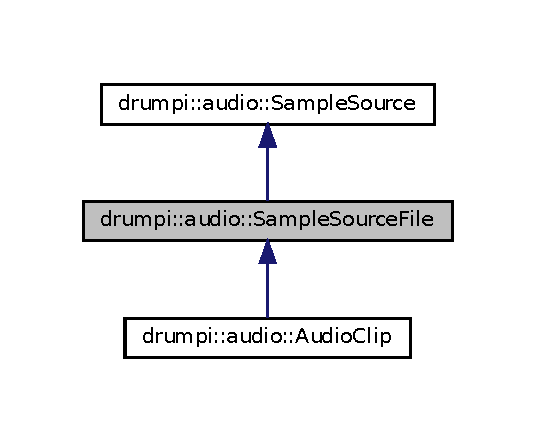
\includegraphics[width=257pt]{classdrumpi_1_1audio_1_1SampleSourceFile__inherit__graph}
\end{center}
\end{figure}


Collaboration diagram for drumpi\+::audio\+::Sample\+Source\+File\+:\nopagebreak
\begin{figure}[H]
\begin{center}
\leavevmode
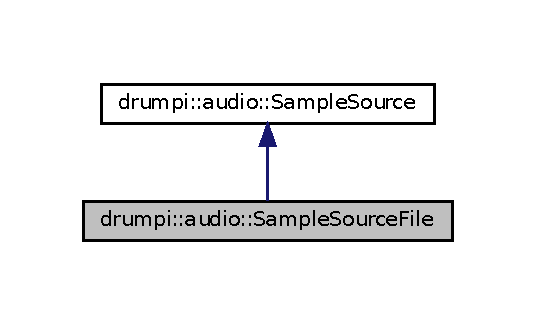
\includegraphics[width=257pt]{classdrumpi_1_1audio_1_1SampleSourceFile__coll__graph}
\end{center}
\end{figure}
\doxysubsection*{Protected Member Functions}
\begin{DoxyCompactItemize}
\item 
virtual void \mbox{\hyperlink{classdrumpi_1_1audio_1_1SampleSourceFile_a3a919325368cd163435f5ea6ad9fd4ec}{load\+File}} (std\+::string \mbox{\hyperlink{classdrumpi_1_1audio_1_1SampleSourceFile_a0d6461310f720bf9a25e7c274f57053b}{filepath}})=0
\end{DoxyCompactItemize}
\doxysubsection*{Protected Attributes}
\begin{DoxyCompactItemize}
\item 
std\+::string \mbox{\hyperlink{classdrumpi_1_1audio_1_1SampleSourceFile_a0d6461310f720bf9a25e7c274f57053b}{filepath}}
\end{DoxyCompactItemize}
\doxysubsection*{Additional Inherited Members}


\doxysubsection{Detailed Description}
Specialised abstract class for file-\/based sample sources, e.\+g. wave files. 

\doxysubsection{Member Function Documentation}
\mbox{\Hypertarget{classdrumpi_1_1audio_1_1SampleSourceFile_a3a919325368cd163435f5ea6ad9fd4ec}\label{classdrumpi_1_1audio_1_1SampleSourceFile_a3a919325368cd163435f5ea6ad9fd4ec}} 
\index{drumpi::audio::SampleSourceFile@{drumpi::audio::SampleSourceFile}!loadFile@{loadFile}}
\index{loadFile@{loadFile}!drumpi::audio::SampleSourceFile@{drumpi::audio::SampleSourceFile}}
\doxysubsubsection{\texorpdfstring{loadFile()}{loadFile()}}
{\footnotesize\ttfamily virtual void drumpi\+::audio\+::\+Sample\+Source\+File\+::load\+File (\begin{DoxyParamCaption}\item[{std\+::string}]{filepath }\end{DoxyParamCaption})\hspace{0.3cm}{\ttfamily [protected]}, {\ttfamily [pure virtual]}}

Loads the specified file. 
\begin{DoxyParams}{Parameters}
{\em filepath} & file path of the file to load. \\
\hline
\end{DoxyParams}


Implemented in \mbox{\hyperlink{classdrumpi_1_1audio_1_1AudioClip_af00b5d353bec63b6bbbbe58509b95fe3}{drumpi\+::audio\+::\+Audio\+Clip}}.



\doxysubsection{Member Data Documentation}
\mbox{\Hypertarget{classdrumpi_1_1audio_1_1SampleSourceFile_a0d6461310f720bf9a25e7c274f57053b}\label{classdrumpi_1_1audio_1_1SampleSourceFile_a0d6461310f720bf9a25e7c274f57053b}} 
\index{drumpi::audio::SampleSourceFile@{drumpi::audio::SampleSourceFile}!filepath@{filepath}}
\index{filepath@{filepath}!drumpi::audio::SampleSourceFile@{drumpi::audio::SampleSourceFile}}
\doxysubsubsection{\texorpdfstring{filepath}{filepath}}
{\footnotesize\ttfamily std\+::string drumpi\+::audio\+::\+Sample\+Source\+File\+::filepath\hspace{0.3cm}{\ttfamily [protected]}}

File path used for loading. 

The documentation for this class was generated from the following file\+:\begin{DoxyCompactItemize}
\item 
src/sample\+Source.\+hpp\end{DoxyCompactItemize}

\hypertarget{classdrumpi_1_1Sequencer}{}\doxysection{drumpi\+::Sequencer Class Reference}
\label{classdrumpi_1_1Sequencer}\index{drumpi::Sequencer@{drumpi::Sequencer}}


{\ttfamily \#include $<$sequencer.\+hpp$>$}



Collaboration diagram for drumpi\+::Sequencer\+:\nopagebreak
\begin{figure}[H]
\begin{center}
\leavevmode
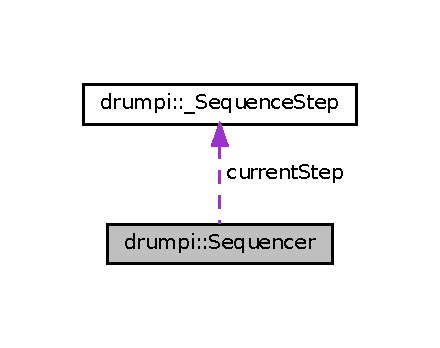
\includegraphics[width=211pt]{classdrumpi_1_1Sequencer__coll__graph}
\end{center}
\end{figure}
\doxysubsection*{Public Member Functions}
\begin{DoxyCompactItemize}
\item 
\mbox{\hyperlink{classdrumpi_1_1Sequencer_ae1c19c8eadf10ac7ef53fa9b8b9d36e9}{Sequencer}} (const int \mbox{\hyperlink{classdrumpi_1_1Sequencer_a0e4963cb16a4c6cbeb85838199c1bb8e}{num\+Steps}})
\item 
void \mbox{\hyperlink{classdrumpi_1_1Sequencer_a86e0af4260c526be4646ce343830e6c4}{step}} (int n=1)
\item 
bool \mbox{\hyperlink{classdrumpi_1_1Sequencer_a9125b926864c998496a662b1fd8cd535}{is\+Active}} (\mbox{\hyperlink{namespacedrumpi_ad560bde7b693769d2c5882437af094bf}{drum\+I\+D\+\_\+t}} drum, int \mbox{\hyperlink{classdrumpi_1_1Sequencer_a86e0af4260c526be4646ce343830e6c4}{step}})
\item 
bool \mbox{\hyperlink{classdrumpi_1_1Sequencer_a7af390c7241b0fc7ccdf17cd6f14171f}{is\+Active}} (\mbox{\hyperlink{namespacedrumpi_ad560bde7b693769d2c5882437af094bf}{drum\+I\+D\+\_\+t}} drum)
\item 
std\+::vector$<$ \mbox{\hyperlink{namespacedrumpi_ad560bde7b693769d2c5882437af094bf}{drum\+I\+D\+\_\+t}} $>$ \mbox{\hyperlink{classdrumpi_1_1Sequencer_a3a4981971243ac03ace9b57fc0a6c8c6}{get\+Active}} ()
\item 
std\+::vector$<$ bool $>$ \mbox{\hyperlink{classdrumpi_1_1Sequencer_a5cc5ed8f6fd51b88618766a16373b60d}{get\+Steps}} (\mbox{\hyperlink{namespacedrumpi_ad560bde7b693769d2c5882437af094bf}{drum\+I\+D\+\_\+t}} drum\+ID)
\item 
std\+::vector$<$ std\+::vector$<$ bool $>$ $>$ \mbox{\hyperlink{classdrumpi_1_1Sequencer_aa15ac653eaddea48cb4ccb8dadac9735}{get\+Sequence}} ()
\item 
int \mbox{\hyperlink{classdrumpi_1_1Sequencer_af327472b3452fa67511029daaee4ad1c}{get\+Step\+Num}} ()
\item 
void \mbox{\hyperlink{classdrumpi_1_1Sequencer_a8b7b4faa1438aedb59370bb5ef44f571}{clear}} ()
\item 
void \mbox{\hyperlink{classdrumpi_1_1Sequencer_a033983bb65fa38a3e0f8732040a63eb1}{reset}} (bool clear\+Steps=true)
\item 
void \mbox{\hyperlink{classdrumpi_1_1Sequencer_abf7916305c8766c01b3dc0230012cf3d}{add}} (\mbox{\hyperlink{namespacedrumpi_ad560bde7b693769d2c5882437af094bf}{drum\+I\+D\+\_\+t}} drum, int \mbox{\hyperlink{classdrumpi_1_1Sequencer_a86e0af4260c526be4646ce343830e6c4}{step}})
\item 
void \mbox{\hyperlink{classdrumpi_1_1Sequencer_a65d14581132cc9ece12eca56a1696e27}{add}} (\mbox{\hyperlink{namespacedrumpi_ad560bde7b693769d2c5882437af094bf}{drum\+I\+D\+\_\+t}} drum)
\item 
void \mbox{\hyperlink{classdrumpi_1_1Sequencer_a5b9b8acf415b43f72442f0a591054412}{remove}} (\mbox{\hyperlink{namespacedrumpi_ad560bde7b693769d2c5882437af094bf}{drum\+I\+D\+\_\+t}} drum, int \mbox{\hyperlink{classdrumpi_1_1Sequencer_a86e0af4260c526be4646ce343830e6c4}{step}})
\item 
void \mbox{\hyperlink{classdrumpi_1_1Sequencer_ad7fcb2041b2b68133def003eef420f99}{remove}} (\mbox{\hyperlink{namespacedrumpi_ad560bde7b693769d2c5882437af094bf}{drum\+I\+D\+\_\+t}} drum)
\item 
void \mbox{\hyperlink{classdrumpi_1_1Sequencer_a2d7b85fe97bd2714632bd65135868897}{toggle}} (\mbox{\hyperlink{namespacedrumpi_ad560bde7b693769d2c5882437af094bf}{drum\+I\+D\+\_\+t}} drum, int \mbox{\hyperlink{classdrumpi_1_1Sequencer_a86e0af4260c526be4646ce343830e6c4}{step}})
\item 
void \mbox{\hyperlink{classdrumpi_1_1Sequencer_a7ca8d490e9eaf703c9f7e0594fa4090c}{toggle}} (\mbox{\hyperlink{namespacedrumpi_ad560bde7b693769d2c5882437af094bf}{drum\+I\+D\+\_\+t}} drum)
\end{DoxyCompactItemize}
\doxysubsection*{Private Member Functions}
\begin{DoxyCompactItemize}
\item 
void \mbox{\hyperlink{classdrumpi_1_1Sequencer_adf7a6603073c345b72805211f87d5d1c}{set\+Num\+Steps}} (int n)
\item 
void \mbox{\hyperlink{classdrumpi_1_1Sequencer_a55a080037b948534ef6fab28ee3cf8e1}{\+\_\+update\+Step\+ID}} ()
\item 
void \mbox{\hyperlink{classdrumpi_1_1Sequencer_a3d07f2cafd5fc311aa05e049685756e4}{\+\_\+update\+Step\+Ptr}} ()
\end{DoxyCompactItemize}
\doxysubsection*{Private Attributes}
\begin{DoxyCompactItemize}
\item 
std\+::vector$<$ \mbox{\hyperlink{classdrumpi_1_1__SequenceStep}{\+\_\+\+Sequence\+Step}} $>$ \mbox{\hyperlink{classdrumpi_1_1Sequencer_a756f8ef45e87ef2165d7e34752c9bf7e}{steps}}
\item 
int \mbox{\hyperlink{classdrumpi_1_1Sequencer_a0e4963cb16a4c6cbeb85838199c1bb8e}{num\+Steps}}
\item 
int \mbox{\hyperlink{classdrumpi_1_1Sequencer_a259a1eb2adc67dc949c2cdb45358886d}{step\+Num}}
\item 
\mbox{\hyperlink{classdrumpi_1_1__SequenceStep}{\+\_\+\+Sequence\+Step}} $\ast$ \mbox{\hyperlink{classdrumpi_1_1Sequencer_a0bf12baf6bf923324df41f1ea784ba99}{current\+Step}}
\end{DoxyCompactItemize}


\doxysubsection{Detailed Description}
\mbox{\hyperlink{classdrumpi_1_1Sequencer}{Sequencer}} class for creating, manipulating and outputting a drum sequence. 

\doxysubsection{Constructor \& Destructor Documentation}
\mbox{\Hypertarget{classdrumpi_1_1Sequencer_ae1c19c8eadf10ac7ef53fa9b8b9d36e9}\label{classdrumpi_1_1Sequencer_ae1c19c8eadf10ac7ef53fa9b8b9d36e9}} 
\index{drumpi::Sequencer@{drumpi::Sequencer}!Sequencer@{Sequencer}}
\index{Sequencer@{Sequencer}!drumpi::Sequencer@{drumpi::Sequencer}}
\doxysubsubsection{\texorpdfstring{Sequencer()}{Sequencer()}}
{\footnotesize\ttfamily Sequencer\+::\+Sequencer (\begin{DoxyParamCaption}\item[{const int}]{num\+Steps }\end{DoxyParamCaption})}

Constructor. 
\begin{DoxyParams}{Parameters}
{\em num\+Steps} & the number of steps in the sequence. \\
\hline
\end{DoxyParams}


\doxysubsection{Member Function Documentation}
\mbox{\Hypertarget{classdrumpi_1_1Sequencer_a55a080037b948534ef6fab28ee3cf8e1}\label{classdrumpi_1_1Sequencer_a55a080037b948534ef6fab28ee3cf8e1}} 
\index{drumpi::Sequencer@{drumpi::Sequencer}!\_updateStepID@{\_updateStepID}}
\index{\_updateStepID@{\_updateStepID}!drumpi::Sequencer@{drumpi::Sequencer}}
\doxysubsubsection{\texorpdfstring{\_updateStepID()}{\_updateStepID()}}
{\footnotesize\ttfamily void Sequencer\+::\+\_\+update\+Step\+ID (\begin{DoxyParamCaption}{ }\end{DoxyParamCaption})\hspace{0.3cm}{\ttfamily [private]}}

Call to update the active step ID. \mbox{\Hypertarget{classdrumpi_1_1Sequencer_a3d07f2cafd5fc311aa05e049685756e4}\label{classdrumpi_1_1Sequencer_a3d07f2cafd5fc311aa05e049685756e4}} 
\index{drumpi::Sequencer@{drumpi::Sequencer}!\_updateStepPtr@{\_updateStepPtr}}
\index{\_updateStepPtr@{\_updateStepPtr}!drumpi::Sequencer@{drumpi::Sequencer}}
\doxysubsubsection{\texorpdfstring{\_updateStepPtr()}{\_updateStepPtr()}}
{\footnotesize\ttfamily void Sequencer\+::\+\_\+update\+Step\+Ptr (\begin{DoxyParamCaption}{ }\end{DoxyParamCaption})\hspace{0.3cm}{\ttfamily [private]}}

Call to update the active step pointer. Should be called after the active step ID is updated (see \mbox{\hyperlink{classdrumpi_1_1Sequencer_a55a080037b948534ef6fab28ee3cf8e1}{\+\_\+update\+Step\+ID}}). \mbox{\Hypertarget{classdrumpi_1_1Sequencer_a65d14581132cc9ece12eca56a1696e27}\label{classdrumpi_1_1Sequencer_a65d14581132cc9ece12eca56a1696e27}} 
\index{drumpi::Sequencer@{drumpi::Sequencer}!add@{add}}
\index{add@{add}!drumpi::Sequencer@{drumpi::Sequencer}}
\doxysubsubsection{\texorpdfstring{add()}{add()}\hspace{0.1cm}{\footnotesize\ttfamily [1/2]}}
{\footnotesize\ttfamily void Sequencer\+::add (\begin{DoxyParamCaption}\item[{\mbox{\hyperlink{namespacedrumpi_ad560bde7b693769d2c5882437af094bf}{drum\+I\+D\+\_\+t}}}]{drum }\end{DoxyParamCaption})}

Adds the specified drum to the current step. 
\begin{DoxyParams}{Parameters}
{\em drum} & \mbox{\hyperlink{namespacedrumpi_ad560bde7b693769d2c5882437af094bf}{drum\+I\+D\+\_\+t}} of the drum to add. \\
\hline
\end{DoxyParams}
\mbox{\Hypertarget{classdrumpi_1_1Sequencer_abf7916305c8766c01b3dc0230012cf3d}\label{classdrumpi_1_1Sequencer_abf7916305c8766c01b3dc0230012cf3d}} 
\index{drumpi::Sequencer@{drumpi::Sequencer}!add@{add}}
\index{add@{add}!drumpi::Sequencer@{drumpi::Sequencer}}
\doxysubsubsection{\texorpdfstring{add()}{add()}\hspace{0.1cm}{\footnotesize\ttfamily [2/2]}}
{\footnotesize\ttfamily void Sequencer\+::add (\begin{DoxyParamCaption}\item[{\mbox{\hyperlink{namespacedrumpi_ad560bde7b693769d2c5882437af094bf}{drum\+I\+D\+\_\+t}}}]{drum,  }\item[{int}]{step }\end{DoxyParamCaption})}

Adds the specified drum to the specified step. 
\begin{DoxyParams}{Parameters}
{\em drum} & \mbox{\hyperlink{namespacedrumpi_ad560bde7b693769d2c5882437af094bf}{drum\+I\+D\+\_\+t}} of the drum to add. \\
\hline
{\em step} & ID of the step to be modified. \\
\hline
\end{DoxyParams}
\mbox{\Hypertarget{classdrumpi_1_1Sequencer_a8b7b4faa1438aedb59370bb5ef44f571}\label{classdrumpi_1_1Sequencer_a8b7b4faa1438aedb59370bb5ef44f571}} 
\index{drumpi::Sequencer@{drumpi::Sequencer}!clear@{clear}}
\index{clear@{clear}!drumpi::Sequencer@{drumpi::Sequencer}}
\doxysubsubsection{\texorpdfstring{clear()}{clear()}}
{\footnotesize\ttfamily void Sequencer\+::clear (\begin{DoxyParamCaption}{ }\end{DoxyParamCaption})}

Clear the \mbox{\hyperlink{classdrumpi_1_1Sequencer}{Sequencer}} pattern. \mbox{\Hypertarget{classdrumpi_1_1Sequencer_a3a4981971243ac03ace9b57fc0a6c8c6}\label{classdrumpi_1_1Sequencer_a3a4981971243ac03ace9b57fc0a6c8c6}} 
\index{drumpi::Sequencer@{drumpi::Sequencer}!getActive@{getActive}}
\index{getActive@{getActive}!drumpi::Sequencer@{drumpi::Sequencer}}
\doxysubsubsection{\texorpdfstring{getActive()}{getActive()}}
{\footnotesize\ttfamily std\+::vector$<$ \mbox{\hyperlink{namespacedrumpi_ad560bde7b693769d2c5882437af094bf}{drum\+I\+D\+\_\+t}} $>$ Sequencer\+::get\+Active (\begin{DoxyParamCaption}{ }\end{DoxyParamCaption})}

Returns the active drums\textquotesingle{} \mbox{\hyperlink{namespacedrumpi_ad560bde7b693769d2c5882437af094bf}{drum\+I\+D\+\_\+t}} for the current step. \begin{DoxyReturn}{Returns}
a vector containing the \mbox{\hyperlink{namespacedrumpi_ad560bde7b693769d2c5882437af094bf}{drum\+I\+D\+\_\+t}} of the active drums. 
\end{DoxyReturn}
\mbox{\Hypertarget{classdrumpi_1_1Sequencer_aa15ac653eaddea48cb4ccb8dadac9735}\label{classdrumpi_1_1Sequencer_aa15ac653eaddea48cb4ccb8dadac9735}} 
\index{drumpi::Sequencer@{drumpi::Sequencer}!getSequence@{getSequence}}
\index{getSequence@{getSequence}!drumpi::Sequencer@{drumpi::Sequencer}}
\doxysubsubsection{\texorpdfstring{getSequence()}{getSequence()}}
{\footnotesize\ttfamily std\+::vector$<$ std\+::vector$<$ bool $>$ $>$ Sequencer\+::get\+Sequence (\begin{DoxyParamCaption}{ }\end{DoxyParamCaption})}

Returns the entire \mbox{\hyperlink{classdrumpi_1_1Sequencer}{Sequencer}} pattern. \begin{DoxyReturn}{Returns}
a 2D vector of the \mbox{\hyperlink{classdrumpi_1_1Sequencer}{Sequencer}} pattern, indexed as \mbox{[}step\mbox{]}\mbox{[}drum\mbox{]}. 
\end{DoxyReturn}
\mbox{\Hypertarget{classdrumpi_1_1Sequencer_af327472b3452fa67511029daaee4ad1c}\label{classdrumpi_1_1Sequencer_af327472b3452fa67511029daaee4ad1c}} 
\index{drumpi::Sequencer@{drumpi::Sequencer}!getStepNum@{getStepNum}}
\index{getStepNum@{getStepNum}!drumpi::Sequencer@{drumpi::Sequencer}}
\doxysubsubsection{\texorpdfstring{getStepNum()}{getStepNum()}}
{\footnotesize\ttfamily int Sequencer\+::get\+Step\+Num (\begin{DoxyParamCaption}{ }\end{DoxyParamCaption})}

Get the current step number. \begin{DoxyReturn}{Returns}
the current step number. 
\end{DoxyReturn}
\mbox{\Hypertarget{classdrumpi_1_1Sequencer_a5cc5ed8f6fd51b88618766a16373b60d}\label{classdrumpi_1_1Sequencer_a5cc5ed8f6fd51b88618766a16373b60d}} 
\index{drumpi::Sequencer@{drumpi::Sequencer}!getSteps@{getSteps}}
\index{getSteps@{getSteps}!drumpi::Sequencer@{drumpi::Sequencer}}
\doxysubsubsection{\texorpdfstring{getSteps()}{getSteps()}}
{\footnotesize\ttfamily std\+::vector$<$ bool $>$ Sequencer\+::get\+Steps (\begin{DoxyParamCaption}\item[{\mbox{\hyperlink{namespacedrumpi_ad560bde7b693769d2c5882437af094bf}{drum\+I\+D\+\_\+t}}}]{drum\+ID }\end{DoxyParamCaption})}

Returns a series of switches for the specified drum\textquotesingle{}s presence in each sequence step. 
\begin{DoxyParams}{Parameters}
{\em drum\+ID} & \mbox{\hyperlink{namespacedrumpi_ad560bde7b693769d2c5882437af094bf}{drum\+I\+D\+\_\+t}} of the drum to check. \\
\hline
\end{DoxyParams}
\begin{DoxyReturn}{Returns}
a vector of {\ttfamily bool}s, {\ttfamily true} if the drum is active in that index\textquotesingle{} step. 
\end{DoxyReturn}
\mbox{\Hypertarget{classdrumpi_1_1Sequencer_a7af390c7241b0fc7ccdf17cd6f14171f}\label{classdrumpi_1_1Sequencer_a7af390c7241b0fc7ccdf17cd6f14171f}} 
\index{drumpi::Sequencer@{drumpi::Sequencer}!isActive@{isActive}}
\index{isActive@{isActive}!drumpi::Sequencer@{drumpi::Sequencer}}
\doxysubsubsection{\texorpdfstring{isActive()}{isActive()}\hspace{0.1cm}{\footnotesize\ttfamily [1/2]}}
{\footnotesize\ttfamily bool Sequencer\+::is\+Active (\begin{DoxyParamCaption}\item[{\mbox{\hyperlink{namespacedrumpi_ad560bde7b693769d2c5882437af094bf}{drum\+I\+D\+\_\+t}}}]{drum }\end{DoxyParamCaption})}

Returns {\ttfamily true} if the specified drum is active in the current step. 
\begin{DoxyParams}{Parameters}
{\em drum} & \mbox{\hyperlink{namespacedrumpi_ad560bde7b693769d2c5882437af094bf}{drum\+I\+D\+\_\+t}} of the drum to test. \\
\hline
\end{DoxyParams}
\mbox{\Hypertarget{classdrumpi_1_1Sequencer_a9125b926864c998496a662b1fd8cd535}\label{classdrumpi_1_1Sequencer_a9125b926864c998496a662b1fd8cd535}} 
\index{drumpi::Sequencer@{drumpi::Sequencer}!isActive@{isActive}}
\index{isActive@{isActive}!drumpi::Sequencer@{drumpi::Sequencer}}
\doxysubsubsection{\texorpdfstring{isActive()}{isActive()}\hspace{0.1cm}{\footnotesize\ttfamily [2/2]}}
{\footnotesize\ttfamily bool Sequencer\+::is\+Active (\begin{DoxyParamCaption}\item[{\mbox{\hyperlink{namespacedrumpi_ad560bde7b693769d2c5882437af094bf}{drum\+I\+D\+\_\+t}}}]{drum,  }\item[{int}]{step }\end{DoxyParamCaption})}

Returns {\ttfamily true} if the specified drum is active in the specified step. 
\begin{DoxyParams}{Parameters}
{\em drum} & \mbox{\hyperlink{namespacedrumpi_ad560bde7b693769d2c5882437af094bf}{drum\+I\+D\+\_\+t}} of the drum to test. \\
\hline
{\em step} & ID of the step to test. \\
\hline
\end{DoxyParams}
\mbox{\Hypertarget{classdrumpi_1_1Sequencer_ad7fcb2041b2b68133def003eef420f99}\label{classdrumpi_1_1Sequencer_ad7fcb2041b2b68133def003eef420f99}} 
\index{drumpi::Sequencer@{drumpi::Sequencer}!remove@{remove}}
\index{remove@{remove}!drumpi::Sequencer@{drumpi::Sequencer}}
\doxysubsubsection{\texorpdfstring{remove()}{remove()}\hspace{0.1cm}{\footnotesize\ttfamily [1/2]}}
{\footnotesize\ttfamily void Sequencer\+::remove (\begin{DoxyParamCaption}\item[{\mbox{\hyperlink{namespacedrumpi_ad560bde7b693769d2c5882437af094bf}{drum\+I\+D\+\_\+t}}}]{drum }\end{DoxyParamCaption})}

Removes the specified drum from the current step. 
\begin{DoxyParams}{Parameters}
{\em drum} & \mbox{\hyperlink{namespacedrumpi_ad560bde7b693769d2c5882437af094bf}{drum\+I\+D\+\_\+t}} of the drum to remove. \\
\hline
\end{DoxyParams}
\mbox{\Hypertarget{classdrumpi_1_1Sequencer_a5b9b8acf415b43f72442f0a591054412}\label{classdrumpi_1_1Sequencer_a5b9b8acf415b43f72442f0a591054412}} 
\index{drumpi::Sequencer@{drumpi::Sequencer}!remove@{remove}}
\index{remove@{remove}!drumpi::Sequencer@{drumpi::Sequencer}}
\doxysubsubsection{\texorpdfstring{remove()}{remove()}\hspace{0.1cm}{\footnotesize\ttfamily [2/2]}}
{\footnotesize\ttfamily void Sequencer\+::remove (\begin{DoxyParamCaption}\item[{\mbox{\hyperlink{namespacedrumpi_ad560bde7b693769d2c5882437af094bf}{drum\+I\+D\+\_\+t}}}]{drum,  }\item[{int}]{step }\end{DoxyParamCaption})}

Removes the specified drum from the specified step. 
\begin{DoxyParams}{Parameters}
{\em drum} & \mbox{\hyperlink{namespacedrumpi_ad560bde7b693769d2c5882437af094bf}{drum\+I\+D\+\_\+t}} of the drum to remove. \\
\hline
{\em step} & ID of the step to be modified. \\
\hline
\end{DoxyParams}
\mbox{\Hypertarget{classdrumpi_1_1Sequencer_a033983bb65fa38a3e0f8732040a63eb1}\label{classdrumpi_1_1Sequencer_a033983bb65fa38a3e0f8732040a63eb1}} 
\index{drumpi::Sequencer@{drumpi::Sequencer}!reset@{reset}}
\index{reset@{reset}!drumpi::Sequencer@{drumpi::Sequencer}}
\doxysubsubsection{\texorpdfstring{reset()}{reset()}}
{\footnotesize\ttfamily void Sequencer\+::reset (\begin{DoxyParamCaption}\item[{bool}]{clear\+Steps = {\ttfamily true} }\end{DoxyParamCaption})}

Resets the \mbox{\hyperlink{classdrumpi_1_1Sequencer}{Sequencer}} to initial conditions. 
\begin{DoxyParams}{Parameters}
{\em clear\+Steps} & whether to clear the \mbox{\hyperlink{classdrumpi_1_1Sequencer}{Sequencer}} pattern. \\
\hline
\end{DoxyParams}
\mbox{\Hypertarget{classdrumpi_1_1Sequencer_adf7a6603073c345b72805211f87d5d1c}\label{classdrumpi_1_1Sequencer_adf7a6603073c345b72805211f87d5d1c}} 
\index{drumpi::Sequencer@{drumpi::Sequencer}!setNumSteps@{setNumSteps}}
\index{setNumSteps@{setNumSteps}!drumpi::Sequencer@{drumpi::Sequencer}}
\doxysubsubsection{\texorpdfstring{setNumSteps()}{setNumSteps()}}
{\footnotesize\ttfamily void Sequencer\+::set\+Num\+Steps (\begin{DoxyParamCaption}\item[{int}]{n }\end{DoxyParamCaption})\hspace{0.3cm}{\ttfamily [private]}}

Sets the number of steps. Unstable for active use. 
\begin{DoxyParams}{Parameters}
{\em n} & desired number of sequence steps. \\
\hline
\end{DoxyParams}
\mbox{\Hypertarget{classdrumpi_1_1Sequencer_a86e0af4260c526be4646ce343830e6c4}\label{classdrumpi_1_1Sequencer_a86e0af4260c526be4646ce343830e6c4}} 
\index{drumpi::Sequencer@{drumpi::Sequencer}!step@{step}}
\index{step@{step}!drumpi::Sequencer@{drumpi::Sequencer}}
\doxysubsubsection{\texorpdfstring{step()}{step()}}
{\footnotesize\ttfamily void Sequencer\+::step (\begin{DoxyParamCaption}\item[{int}]{n = {\ttfamily 1} }\end{DoxyParamCaption})}

Advance the \mbox{\hyperlink{classdrumpi_1_1Sequencer}{Sequencer}} by one step. 
\begin{DoxyParams}{Parameters}
{\em n} & number of step(s) to advance by. \\
\hline
\end{DoxyParams}
\mbox{\Hypertarget{classdrumpi_1_1Sequencer_a7ca8d490e9eaf703c9f7e0594fa4090c}\label{classdrumpi_1_1Sequencer_a7ca8d490e9eaf703c9f7e0594fa4090c}} 
\index{drumpi::Sequencer@{drumpi::Sequencer}!toggle@{toggle}}
\index{toggle@{toggle}!drumpi::Sequencer@{drumpi::Sequencer}}
\doxysubsubsection{\texorpdfstring{toggle()}{toggle()}\hspace{0.1cm}{\footnotesize\ttfamily [1/2]}}
{\footnotesize\ttfamily void Sequencer\+::toggle (\begin{DoxyParamCaption}\item[{\mbox{\hyperlink{namespacedrumpi_ad560bde7b693769d2c5882437af094bf}{drum\+I\+D\+\_\+t}}}]{drum }\end{DoxyParamCaption})}

Toggles the specified drum in the current step. 
\begin{DoxyParams}{Parameters}
{\em drum} & \mbox{\hyperlink{namespacedrumpi_ad560bde7b693769d2c5882437af094bf}{drum\+I\+D\+\_\+t}} of the drum to toggle. \\
\hline
\end{DoxyParams}
\mbox{\Hypertarget{classdrumpi_1_1Sequencer_a2d7b85fe97bd2714632bd65135868897}\label{classdrumpi_1_1Sequencer_a2d7b85fe97bd2714632bd65135868897}} 
\index{drumpi::Sequencer@{drumpi::Sequencer}!toggle@{toggle}}
\index{toggle@{toggle}!drumpi::Sequencer@{drumpi::Sequencer}}
\doxysubsubsection{\texorpdfstring{toggle()}{toggle()}\hspace{0.1cm}{\footnotesize\ttfamily [2/2]}}
{\footnotesize\ttfamily void Sequencer\+::toggle (\begin{DoxyParamCaption}\item[{\mbox{\hyperlink{namespacedrumpi_ad560bde7b693769d2c5882437af094bf}{drum\+I\+D\+\_\+t}}}]{drum,  }\item[{int}]{step }\end{DoxyParamCaption})}

Toggles the specified drum in the specified step. 
\begin{DoxyParams}{Parameters}
{\em drum} & \mbox{\hyperlink{namespacedrumpi_ad560bde7b693769d2c5882437af094bf}{drum\+I\+D\+\_\+t}} of the drum to toggle. \\
\hline
{\em step} & ID of the step to be modified. \\
\hline
\end{DoxyParams}


\doxysubsection{Member Data Documentation}
\mbox{\Hypertarget{classdrumpi_1_1Sequencer_a0bf12baf6bf923324df41f1ea784ba99}\label{classdrumpi_1_1Sequencer_a0bf12baf6bf923324df41f1ea784ba99}} 
\index{drumpi::Sequencer@{drumpi::Sequencer}!currentStep@{currentStep}}
\index{currentStep@{currentStep}!drumpi::Sequencer@{drumpi::Sequencer}}
\doxysubsubsection{\texorpdfstring{currentStep}{currentStep}}
{\footnotesize\ttfamily \mbox{\hyperlink{classdrumpi_1_1__SequenceStep}{\+\_\+\+Sequence\+Step}}$\ast$ drumpi\+::\+Sequencer\+::current\+Step\hspace{0.3cm}{\ttfamily [private]}}

Pointer to currently active \mbox{\hyperlink{classdrumpi_1_1__SequenceStep}{\+\_\+\+Sequence\+Step}} object. \mbox{\Hypertarget{classdrumpi_1_1Sequencer_a0e4963cb16a4c6cbeb85838199c1bb8e}\label{classdrumpi_1_1Sequencer_a0e4963cb16a4c6cbeb85838199c1bb8e}} 
\index{drumpi::Sequencer@{drumpi::Sequencer}!numSteps@{numSteps}}
\index{numSteps@{numSteps}!drumpi::Sequencer@{drumpi::Sequencer}}
\doxysubsubsection{\texorpdfstring{numSteps}{numSteps}}
{\footnotesize\ttfamily int drumpi\+::\+Sequencer\+::num\+Steps\hspace{0.3cm}{\ttfamily [private]}}

Number of steps in the sequence. \mbox{\Hypertarget{classdrumpi_1_1Sequencer_a259a1eb2adc67dc949c2cdb45358886d}\label{classdrumpi_1_1Sequencer_a259a1eb2adc67dc949c2cdb45358886d}} 
\index{drumpi::Sequencer@{drumpi::Sequencer}!stepNum@{stepNum}}
\index{stepNum@{stepNum}!drumpi::Sequencer@{drumpi::Sequencer}}
\doxysubsubsection{\texorpdfstring{stepNum}{stepNum}}
{\footnotesize\ttfamily int drumpi\+::\+Sequencer\+::step\+Num\hspace{0.3cm}{\ttfamily [private]}}

Index of the current step, e.\+g. in the \mbox{\hyperlink{classdrumpi_1_1Sequencer_a756f8ef45e87ef2165d7e34752c9bf7e}{steps}} vector. \mbox{\Hypertarget{classdrumpi_1_1Sequencer_a756f8ef45e87ef2165d7e34752c9bf7e}\label{classdrumpi_1_1Sequencer_a756f8ef45e87ef2165d7e34752c9bf7e}} 
\index{drumpi::Sequencer@{drumpi::Sequencer}!steps@{steps}}
\index{steps@{steps}!drumpi::Sequencer@{drumpi::Sequencer}}
\doxysubsubsection{\texorpdfstring{steps}{steps}}
{\footnotesize\ttfamily std\+::vector$<$\mbox{\hyperlink{classdrumpi_1_1__SequenceStep}{\+\_\+\+Sequence\+Step}}$>$ drumpi\+::\+Sequencer\+::steps\hspace{0.3cm}{\ttfamily [private]}}

Container for \mbox{\hyperlink{classdrumpi_1_1__SequenceStep}{\+\_\+\+Sequence\+Step}} objects. 

The documentation for this class was generated from the following files\+:\begin{DoxyCompactItemize}
\item 
src/sequencer.\+hpp\item 
src/sequencer.\+cpp\end{DoxyCompactItemize}

\hypertarget{classdrumpi_1_1SequencerClock}{}\section{drumpi\+:\+:Sequencer\+Clock Class Reference}
\label{classdrumpi_1_1SequencerClock}\index{drumpi\+::\+Sequencer\+Clock@{drumpi\+::\+Sequencer\+Clock}}


{\ttfamily \#include $<$sequencer.\+hpp$>$}



Inheritance diagram for drumpi\+:\+:Sequencer\+Clock\+:
\nopagebreak
\begin{figure}[H]
\begin{center}
\leavevmode
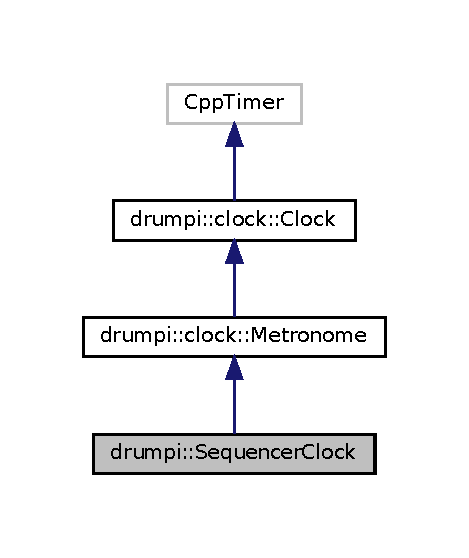
\includegraphics[width=210pt]{classdrumpi_1_1SequencerClock__inherit__graph}
\end{center}
\end{figure}


Collaboration diagram for drumpi\+:\+:Sequencer\+Clock\+:
\nopagebreak
\begin{figure}[H]
\begin{center}
\leavevmode
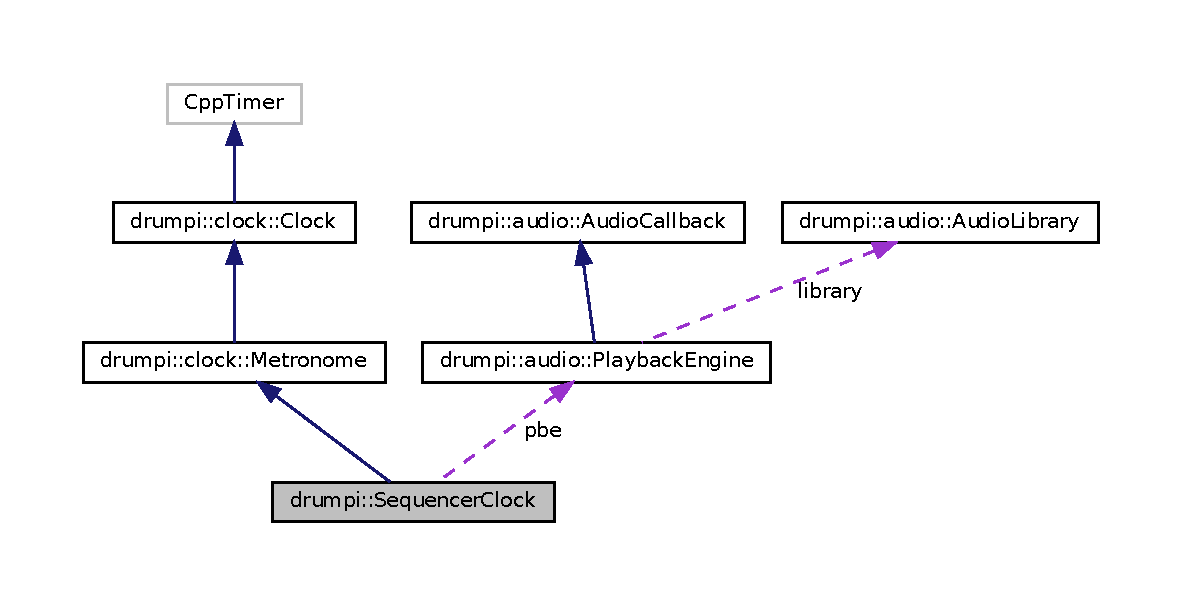
\includegraphics[width=350pt]{classdrumpi_1_1SequencerClock__coll__graph}
\end{center}
\end{figure}
\subsection*{Public Member Functions}
\begin{DoxyCompactItemize}
\item 
\hyperlink{classdrumpi_1_1SequencerClock_a587ae7c0480f05a728b41d99a028c80b}{Sequencer\+Clock} (std\+::shared\+\_\+ptr$<$ \hyperlink{classdrumpi_1_1Sequencer}{Sequencer} $>$ s, \hyperlink{classdrumpi_1_1audio_1_1PlaybackEngine}{audio\+::\+Playback\+Engine} \&p)
\item 
void \hyperlink{classdrumpi_1_1SequencerClock_ac75142ddc2ee0dcd3c52d13e44b0d85f}{tick} () override
\end{DoxyCompactItemize}
\subsection*{Private Attributes}
\begin{DoxyCompactItemize}
\item 
std\+::shared\+\_\+ptr$<$ \hyperlink{classdrumpi_1_1Sequencer}{Sequencer} $>$ \hyperlink{classdrumpi_1_1SequencerClock_aa6dc6e6c44fd5ba2e3a5456db8692915}{seq} = nullptr
\item 
\hyperlink{classdrumpi_1_1audio_1_1PlaybackEngine}{audio\+::\+Playback\+Engine} $\ast$ \hyperlink{classdrumpi_1_1SequencerClock_ae3ec41e6da35975b98942f110dc0e6dc}{pbe}
\end{DoxyCompactItemize}
\subsection*{Additional Inherited Members}


\subsection{Detailed Description}
\hyperlink{classdrumpi_1_1clock_1_1Metronome_acc6e0b5140c79326682ec62eb879bf37}{Metronome} derived class to clock a \hyperlink{classdrumpi_1_1Sequencer}{Sequencer}. 

\subsection{Constructor \& Destructor Documentation}
\mbox{\Hypertarget{classdrumpi_1_1SequencerClock_a587ae7c0480f05a728b41d99a028c80b}\label{classdrumpi_1_1SequencerClock_a587ae7c0480f05a728b41d99a028c80b}} 
\index{drumpi\+::\+Sequencer\+Clock@{drumpi\+::\+Sequencer\+Clock}!Sequencer\+Clock@{Sequencer\+Clock}}
\index{Sequencer\+Clock@{Sequencer\+Clock}!drumpi\+::\+Sequencer\+Clock@{drumpi\+::\+Sequencer\+Clock}}
\subsubsection{\texorpdfstring{Sequencer\+Clock()}{SequencerClock()}}
{\footnotesize\ttfamily Sequencer\+Clock\+::\+Sequencer\+Clock (\begin{DoxyParamCaption}\item[{std\+::shared\+\_\+ptr$<$ \hyperlink{classdrumpi_1_1Sequencer}{Sequencer} $>$}]{s,  }\item[{\hyperlink{classdrumpi_1_1audio_1_1PlaybackEngine}{audio\+::\+Playback\+Engine} \&}]{p }\end{DoxyParamCaption})}

Constructor. Sets the \hyperlink{classdrumpi_1_1Sequencer}{Sequencer} to be clocked. 
\begin{DoxyParams}{Parameters}
{\em s} & \hyperlink{classdrumpi_1_1Sequencer}{Sequencer} object to be clocked. \\
\hline
{\em p} & \hyperlink{classdrumpi_1_1audio_1_1PlaybackEngine}{audio\+::\+Playback\+Engine} object for triggering the active drums. \\
\hline
\end{DoxyParams}


\subsection{Member Function Documentation}
\mbox{\Hypertarget{classdrumpi_1_1SequencerClock_ac75142ddc2ee0dcd3c52d13e44b0d85f}\label{classdrumpi_1_1SequencerClock_ac75142ddc2ee0dcd3c52d13e44b0d85f}} 
\index{drumpi\+::\+Sequencer\+Clock@{drumpi\+::\+Sequencer\+Clock}!tick@{tick}}
\index{tick@{tick}!drumpi\+::\+Sequencer\+Clock@{drumpi\+::\+Sequencer\+Clock}}
\subsubsection{\texorpdfstring{tick()}{tick()}}
{\footnotesize\ttfamily void Sequencer\+Clock\+::tick (\begin{DoxyParamCaption}{ }\end{DoxyParamCaption})\hspace{0.3cm}{\ttfamily [override]}, {\ttfamily [virtual]}}

Override the tick method. Clocks the \hyperlink{classdrumpi_1_1Sequencer}{Sequencer} given to the constructor. 

Implements \hyperlink{classdrumpi_1_1clock_1_1Clock_ade9259c06e6b90bbd92e155a2506d3a1}{drumpi\+::clock\+::\+Clock}.



\subsection{Member Data Documentation}
\mbox{\Hypertarget{classdrumpi_1_1SequencerClock_ae3ec41e6da35975b98942f110dc0e6dc}\label{classdrumpi_1_1SequencerClock_ae3ec41e6da35975b98942f110dc0e6dc}} 
\index{drumpi\+::\+Sequencer\+Clock@{drumpi\+::\+Sequencer\+Clock}!pbe@{pbe}}
\index{pbe@{pbe}!drumpi\+::\+Sequencer\+Clock@{drumpi\+::\+Sequencer\+Clock}}
\subsubsection{\texorpdfstring{pbe}{pbe}}
{\footnotesize\ttfamily \hyperlink{classdrumpi_1_1audio_1_1PlaybackEngine}{audio\+::\+Playback\+Engine}$\ast$ drumpi\+::\+Sequencer\+Clock\+::pbe\hspace{0.3cm}{\ttfamily [private]}}

Pointer to the \hyperlink{classdrumpi_1_1audio_1_1PlaybackEngine}{audio\+::\+Playback\+Engine} used for triggering the active drums. \mbox{\Hypertarget{classdrumpi_1_1SequencerClock_aa6dc6e6c44fd5ba2e3a5456db8692915}\label{classdrumpi_1_1SequencerClock_aa6dc6e6c44fd5ba2e3a5456db8692915}} 
\index{drumpi\+::\+Sequencer\+Clock@{drumpi\+::\+Sequencer\+Clock}!seq@{seq}}
\index{seq@{seq}!drumpi\+::\+Sequencer\+Clock@{drumpi\+::\+Sequencer\+Clock}}
\subsubsection{\texorpdfstring{seq}{seq}}
{\footnotesize\ttfamily std\+::shared\+\_\+ptr$<$\hyperlink{classdrumpi_1_1Sequencer}{Sequencer}$>$ drumpi\+::\+Sequencer\+Clock\+::seq = nullptr\hspace{0.3cm}{\ttfamily [private]}}

Pointer to the \hyperlink{classdrumpi_1_1Sequencer}{Sequencer} object to be clocked. 

The documentation for this class was generated from the following files\+:\begin{DoxyCompactItemize}
\item 
src/sequencer.\+hpp\item 
src/sequencer.\+cpp\end{DoxyCompactItemize}

\hypertarget{classdrumpi_1_1SequencerMode}{}\doxysection{drumpi\+::Sequencer\+Mode Class Reference}
\label{classdrumpi_1_1SequencerMode}\index{drumpi::SequencerMode@{drumpi::SequencerMode}}


{\ttfamily \#include $<$application.\+hpp$>$}



Inheritance diagram for drumpi\+::Sequencer\+Mode\+:\nopagebreak
\begin{figure}[H]
\begin{center}
\leavevmode
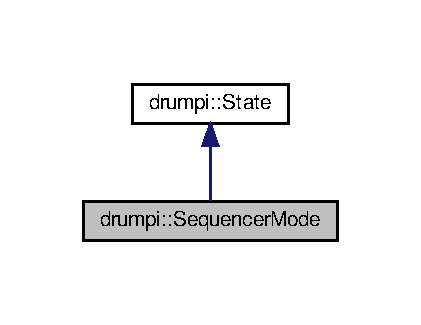
\includegraphics[width=215pt]{classdrumpi_1_1SequencerMode__inherit__graph}
\end{center}
\end{figure}


Collaboration diagram for drumpi\+::Sequencer\+Mode\+:\nopagebreak
\begin{figure}[H]
\begin{center}
\leavevmode
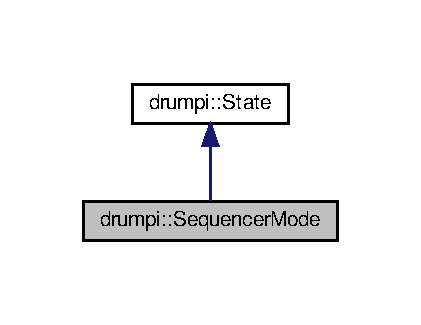
\includegraphics[width=215pt]{classdrumpi_1_1SequencerMode__coll__graph}
\end{center}
\end{figure}
\doxysubsection*{Public Member Functions}
\begin{DoxyCompactItemize}
\item 
\mbox{\hyperlink{classdrumpi_1_1SequencerMode_ae227bba77d671b927514be2cf3fbb0a0}{Sequencer\+Mode}} ()
\item 
bool \mbox{\hyperlink{classdrumpi_1_1SequencerMode_aaa5dea1ffd66792ba62afae00820ffc6}{interpret\+Key\+Press}} (\mbox{\hyperlink{classdrumpi_1_1ApplicationCallback}{Application\+Callback}} $\ast$appc, int key) override
\begin{DoxyCompactList}\small\item\em Performs an action depending on the key pressed. \end{DoxyCompactList}\item 
void \mbox{\hyperlink{classdrumpi_1_1SequencerMode_a0308bc9641daff4f48d74f9d2493d123}{update\+Display}} (\mbox{\hyperlink{classdrumpi_1_1ApplicationCallback}{Application\+Callback}} $\ast$appc) override
\end{DoxyCompactItemize}
\doxysubsection*{Public Attributes}
\begin{DoxyCompactItemize}
\item 
\mbox{\hyperlink{namespacedrumpi_ad560bde7b693769d2c5882437af094bf}{drum\+I\+D\+\_\+t}} \mbox{\hyperlink{classdrumpi_1_1SequencerMode_abc62b03ade3fc568d419584756974aa1}{currentdrum}}
\item 
int \mbox{\hyperlink{classdrumpi_1_1SequencerMode_a3c1fc81b3a46f7df19e1bfa87b7f9bb2}{currentpage}}
\begin{DoxyCompactList}\small\item\em Page currently displayed on Zero\+Seg. \end{DoxyCompactList}\end{DoxyCompactItemize}


\doxysubsection{Detailed Description}
\mbox{\hyperlink{classdrumpi_1_1Sequencer}{Sequencer}} mode state. 

\doxysubsection{Constructor \& Destructor Documentation}
\mbox{\Hypertarget{classdrumpi_1_1SequencerMode_ae227bba77d671b927514be2cf3fbb0a0}\label{classdrumpi_1_1SequencerMode_ae227bba77d671b927514be2cf3fbb0a0}} 
\index{drumpi::SequencerMode@{drumpi::SequencerMode}!SequencerMode@{SequencerMode}}
\index{SequencerMode@{SequencerMode}!drumpi::SequencerMode@{drumpi::SequencerMode}}
\doxysubsubsection{\texorpdfstring{SequencerMode()}{SequencerMode()}}
{\footnotesize\ttfamily Sequencer\+Mode\+::\+Sequencer\+Mode (\begin{DoxyParamCaption}{ }\end{DoxyParamCaption})}

Constructor 

\doxysubsection{Member Function Documentation}
\mbox{\Hypertarget{classdrumpi_1_1SequencerMode_aaa5dea1ffd66792ba62afae00820ffc6}\label{classdrumpi_1_1SequencerMode_aaa5dea1ffd66792ba62afae00820ffc6}} 
\index{drumpi::SequencerMode@{drumpi::SequencerMode}!interpretKeyPress@{interpretKeyPress}}
\index{interpretKeyPress@{interpretKeyPress}!drumpi::SequencerMode@{drumpi::SequencerMode}}
\doxysubsubsection{\texorpdfstring{interpretKeyPress()}{interpretKeyPress()}}
{\footnotesize\ttfamily bool Sequencer\+Mode\+::interpret\+Key\+Press (\begin{DoxyParamCaption}\item[{\mbox{\hyperlink{classdrumpi_1_1ApplicationCallback}{Application\+Callback}} $\ast$}]{appc,  }\item[{int}]{key }\end{DoxyParamCaption})\hspace{0.3cm}{\ttfamily [override]}, {\ttfamily [virtual]}}



Performs an action depending on the key pressed. 

This method is called by the \mbox{\hyperlink{classdrumpi_1_1Application}{Application}} when a keyboard event occurs and the application is in sequencer mode. 
\begin{DoxyParams}{Parameters}
{\em appc} & Callback to the main \mbox{\hyperlink{classdrumpi_1_1Application}{Application}}. \\
\hline
{\em key} & The keypress detected. \\
\hline
\end{DoxyParams}


Implements \mbox{\hyperlink{classdrumpi_1_1State_aaa6205d85513b3f717c126e0717e1dbd}{drumpi\+::\+State}}.

\mbox{\Hypertarget{classdrumpi_1_1SequencerMode_a0308bc9641daff4f48d74f9d2493d123}\label{classdrumpi_1_1SequencerMode_a0308bc9641daff4f48d74f9d2493d123}} 
\index{drumpi::SequencerMode@{drumpi::SequencerMode}!updateDisplay@{updateDisplay}}
\index{updateDisplay@{updateDisplay}!drumpi::SequencerMode@{drumpi::SequencerMode}}
\doxysubsubsection{\texorpdfstring{updateDisplay()}{updateDisplay()}}
{\footnotesize\ttfamily void Sequencer\+Mode\+::update\+Display (\begin{DoxyParamCaption}\item[{\mbox{\hyperlink{classdrumpi_1_1ApplicationCallback}{Application\+Callback}} $\ast$}]{appc }\end{DoxyParamCaption})\hspace{0.3cm}{\ttfamily [override]}, {\ttfamily [virtual]}}

Virtual function to be overridden by derived class. 

Implements \mbox{\hyperlink{classdrumpi_1_1State_a400c5fc605ddec1e4fe18c361bf38ef2}{drumpi\+::\+State}}.



\doxysubsection{Member Data Documentation}
\mbox{\Hypertarget{classdrumpi_1_1SequencerMode_abc62b03ade3fc568d419584756974aa1}\label{classdrumpi_1_1SequencerMode_abc62b03ade3fc568d419584756974aa1}} 
\index{drumpi::SequencerMode@{drumpi::SequencerMode}!currentdrum@{currentdrum}}
\index{currentdrum@{currentdrum}!drumpi::SequencerMode@{drumpi::SequencerMode}}
\doxysubsubsection{\texorpdfstring{currentdrum}{currentdrum}}
{\footnotesize\ttfamily \mbox{\hyperlink{namespacedrumpi_ad560bde7b693769d2c5882437af094bf}{drum\+I\+D\+\_\+t}} drumpi\+::\+Sequencer\+Mode\+::currentdrum}

Drum currently being set in sequencer. \mbox{\Hypertarget{classdrumpi_1_1SequencerMode_a3c1fc81b3a46f7df19e1bfa87b7f9bb2}\label{classdrumpi_1_1SequencerMode_a3c1fc81b3a46f7df19e1bfa87b7f9bb2}} 
\index{drumpi::SequencerMode@{drumpi::SequencerMode}!currentpage@{currentpage}}
\index{currentpage@{currentpage}!drumpi::SequencerMode@{drumpi::SequencerMode}}
\doxysubsubsection{\texorpdfstring{currentpage}{currentpage}}
{\footnotesize\ttfamily int drumpi\+::\+Sequencer\+Mode\+::currentpage}



Page currently displayed on Zero\+Seg. 

Either page 1 (beats 1-\/8) or page 2 (beats 9-\/16). 

The documentation for this class was generated from the following files\+:\begin{DoxyCompactItemize}
\item 
src/application.\+hpp\item 
src/application.\+cpp\end{DoxyCompactItemize}

\hypertarget{classdrumpi_1_1SetDrumBankMode}{}\doxysection{drumpi\+::Set\+Drum\+Bank\+Mode Class Reference}
\label{classdrumpi_1_1SetDrumBankMode}\index{drumpi::SetDrumBankMode@{drumpi::SetDrumBankMode}}


{\ttfamily \#include $<$application.\+hpp$>$}



Inheritance diagram for drumpi\+::Set\+Drum\+Bank\+Mode\+:\nopagebreak
\begin{figure}[H]
\begin{center}
\leavevmode
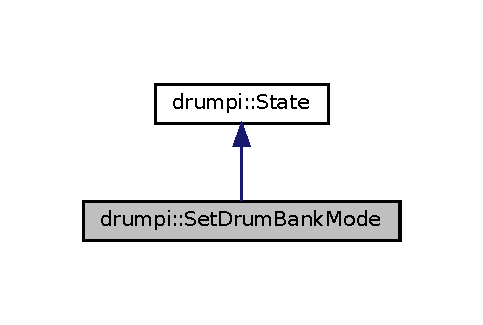
\includegraphics[width=232pt]{classdrumpi_1_1SetDrumBankMode__inherit__graph}
\end{center}
\end{figure}


Collaboration diagram for drumpi\+::Set\+Drum\+Bank\+Mode\+:\nopagebreak
\begin{figure}[H]
\begin{center}
\leavevmode
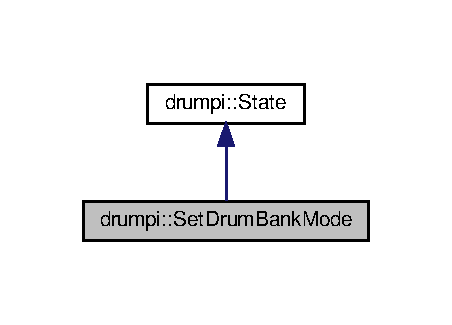
\includegraphics[width=232pt]{classdrumpi_1_1SetDrumBankMode__coll__graph}
\end{center}
\end{figure}
\doxysubsection*{Public Member Functions}
\begin{DoxyCompactItemize}
\item 
\mbox{\hyperlink{classdrumpi_1_1SetDrumBankMode_af0e47a70b3175d10bd31827397c8f0a6}{Set\+Drum\+Bank\+Mode}} ()
\item 
bool \mbox{\hyperlink{classdrumpi_1_1SetDrumBankMode_a9b63a16aa08551a743c3751fa385c83b}{interpret\+Key\+Press}} (\mbox{\hyperlink{classdrumpi_1_1ApplicationCallback}{Application\+Callback}} $\ast$appc, int key) override
\begin{DoxyCompactList}\small\item\em Performs an action depending on the key pressed. \end{DoxyCompactList}\item 
void \mbox{\hyperlink{classdrumpi_1_1SetDrumBankMode_ae2f14f230923c5e0c19c780c59328822}{update\+Display}} (\mbox{\hyperlink{classdrumpi_1_1ApplicationCallback}{Application\+Callback}} $\ast$appc) override
\item 
int \mbox{\hyperlink{classdrumpi_1_1SetDrumBankMode_aa3e8ece8e6a54e9d631d82d6f315f06a}{get\+Bank}} ()
\end{DoxyCompactItemize}
\doxysubsection*{Private Attributes}
\begin{DoxyCompactItemize}
\item 
int \mbox{\hyperlink{classdrumpi_1_1SetDrumBankMode_addef3a7e0513df0ddf7c8d335380d4c7}{bank}}
\item 
int \mbox{\hyperlink{classdrumpi_1_1SetDrumBankMode_a4cec73d2c5ec1cca126220316f800da1}{safe\+Bank}}
\end{DoxyCompactItemize}
\doxysubsection*{Additional Inherited Members}


\doxysubsection{Detailed Description}
Load different banks of drums in this state. 

\doxysubsection{Constructor \& Destructor Documentation}
\mbox{\Hypertarget{classdrumpi_1_1SetDrumBankMode_af0e47a70b3175d10bd31827397c8f0a6}\label{classdrumpi_1_1SetDrumBankMode_af0e47a70b3175d10bd31827397c8f0a6}} 
\index{drumpi::SetDrumBankMode@{drumpi::SetDrumBankMode}!SetDrumBankMode@{SetDrumBankMode}}
\index{SetDrumBankMode@{SetDrumBankMode}!drumpi::SetDrumBankMode@{drumpi::SetDrumBankMode}}
\doxysubsubsection{\texorpdfstring{SetDrumBankMode()}{SetDrumBankMode()}}
{\footnotesize\ttfamily Set\+Drum\+Bank\+Mode\+::\+Set\+Drum\+Bank\+Mode (\begin{DoxyParamCaption}{ }\end{DoxyParamCaption})}

Constructor. 

\doxysubsection{Member Function Documentation}
\mbox{\Hypertarget{classdrumpi_1_1SetDrumBankMode_aa3e8ece8e6a54e9d631d82d6f315f06a}\label{classdrumpi_1_1SetDrumBankMode_aa3e8ece8e6a54e9d631d82d6f315f06a}} 
\index{drumpi::SetDrumBankMode@{drumpi::SetDrumBankMode}!getBank@{getBank}}
\index{getBank@{getBank}!drumpi::SetDrumBankMode@{drumpi::SetDrumBankMode}}
\doxysubsubsection{\texorpdfstring{getBank()}{getBank()}}
{\footnotesize\ttfamily int Set\+Drum\+Bank\+Mode\+::get\+Bank (\begin{DoxyParamCaption}{ }\end{DoxyParamCaption})}

Returns the current bank\textquotesingle{}s ID. \mbox{\Hypertarget{classdrumpi_1_1SetDrumBankMode_a9b63a16aa08551a743c3751fa385c83b}\label{classdrumpi_1_1SetDrumBankMode_a9b63a16aa08551a743c3751fa385c83b}} 
\index{drumpi::SetDrumBankMode@{drumpi::SetDrumBankMode}!interpretKeyPress@{interpretKeyPress}}
\index{interpretKeyPress@{interpretKeyPress}!drumpi::SetDrumBankMode@{drumpi::SetDrumBankMode}}
\doxysubsubsection{\texorpdfstring{interpretKeyPress()}{interpretKeyPress()}}
{\footnotesize\ttfamily bool Set\+Drum\+Bank\+Mode\+::interpret\+Key\+Press (\begin{DoxyParamCaption}\item[{\mbox{\hyperlink{classdrumpi_1_1ApplicationCallback}{Application\+Callback}} $\ast$}]{appc,  }\item[{int}]{key }\end{DoxyParamCaption})\hspace{0.3cm}{\ttfamily [override]}, {\ttfamily [virtual]}}



Performs an action depending on the key pressed. 

This method is called by the \mbox{\hyperlink{classdrumpi_1_1Application}{Application}} when a keyboard event occurs and the application is in \mbox{\hyperlink{classdrumpi_1_1SetDrumBankMode}{Set\+Drum\+Bank\+Mode}}. 
\begin{DoxyParams}{Parameters}
{\em appc} & Callback to the main \mbox{\hyperlink{classdrumpi_1_1Application}{Application}}. \\
\hline
{\em key} & The keypress detected. \\
\hline
\end{DoxyParams}


Implements \mbox{\hyperlink{classdrumpi_1_1State_aaa6205d85513b3f717c126e0717e1dbd}{drumpi\+::\+State}}.

\mbox{\Hypertarget{classdrumpi_1_1SetDrumBankMode_ae2f14f230923c5e0c19c780c59328822}\label{classdrumpi_1_1SetDrumBankMode_ae2f14f230923c5e0c19c780c59328822}} 
\index{drumpi::SetDrumBankMode@{drumpi::SetDrumBankMode}!updateDisplay@{updateDisplay}}
\index{updateDisplay@{updateDisplay}!drumpi::SetDrumBankMode@{drumpi::SetDrumBankMode}}
\doxysubsubsection{\texorpdfstring{updateDisplay()}{updateDisplay()}}
{\footnotesize\ttfamily void Set\+Drum\+Bank\+Mode\+::update\+Display (\begin{DoxyParamCaption}\item[{\mbox{\hyperlink{classdrumpi_1_1ApplicationCallback}{Application\+Callback}} $\ast$}]{appc }\end{DoxyParamCaption})\hspace{0.3cm}{\ttfamily [override]}, {\ttfamily [virtual]}}

Virtual function to be overridden by derived class. 

Implements \mbox{\hyperlink{classdrumpi_1_1State_a400c5fc605ddec1e4fe18c361bf38ef2}{drumpi\+::\+State}}.



\doxysubsection{Member Data Documentation}
\mbox{\Hypertarget{classdrumpi_1_1SetDrumBankMode_addef3a7e0513df0ddf7c8d335380d4c7}\label{classdrumpi_1_1SetDrumBankMode_addef3a7e0513df0ddf7c8d335380d4c7}} 
\index{drumpi::SetDrumBankMode@{drumpi::SetDrumBankMode}!bank@{bank}}
\index{bank@{bank}!drumpi::SetDrumBankMode@{drumpi::SetDrumBankMode}}
\doxysubsubsection{\texorpdfstring{bank}{bank}}
{\footnotesize\ttfamily int drumpi\+::\+Set\+Drum\+Bank\+Mode\+::bank\hspace{0.3cm}{\ttfamily [private]}}

Current bank selected. \mbox{\Hypertarget{classdrumpi_1_1SetDrumBankMode_a4cec73d2c5ec1cca126220316f800da1}\label{classdrumpi_1_1SetDrumBankMode_a4cec73d2c5ec1cca126220316f800da1}} 
\index{drumpi::SetDrumBankMode@{drumpi::SetDrumBankMode}!safeBank@{safeBank}}
\index{safeBank@{safeBank}!drumpi::SetDrumBankMode@{drumpi::SetDrumBankMode}}
\doxysubsubsection{\texorpdfstring{safeBank}{safeBank}}
{\footnotesize\ttfamily int drumpi\+::\+Set\+Drum\+Bank\+Mode\+::safe\+Bank\hspace{0.3cm}{\ttfamily [private]}}

The last bank successfully loaded. 

The documentation for this class was generated from the following files\+:\begin{DoxyCompactItemize}
\item 
src/application.\+hpp\item 
src/application.\+cpp\end{DoxyCompactItemize}

\hypertarget{classdrumpi_1_1SetDrumVolumeMode}{}\doxysection{drumpi\+::Set\+Drum\+Volume\+Mode Class Reference}
\label{classdrumpi_1_1SetDrumVolumeMode}\index{drumpi::SetDrumVolumeMode@{drumpi::SetDrumVolumeMode}}


{\ttfamily \#include $<$application.\+hpp$>$}



Inheritance diagram for drumpi\+::Set\+Drum\+Volume\+Mode\+:\nopagebreak
\begin{figure}[H]
\begin{center}
\leavevmode
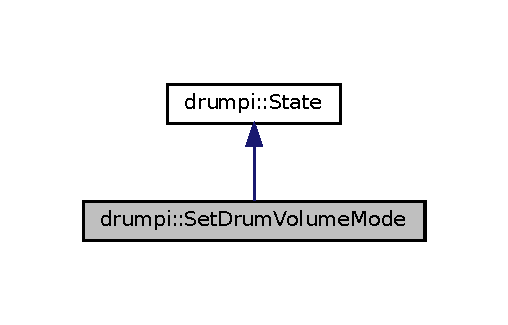
\includegraphics[width=244pt]{classdrumpi_1_1SetDrumVolumeMode__inherit__graph}
\end{center}
\end{figure}


Collaboration diagram for drumpi\+::Set\+Drum\+Volume\+Mode\+:\nopagebreak
\begin{figure}[H]
\begin{center}
\leavevmode
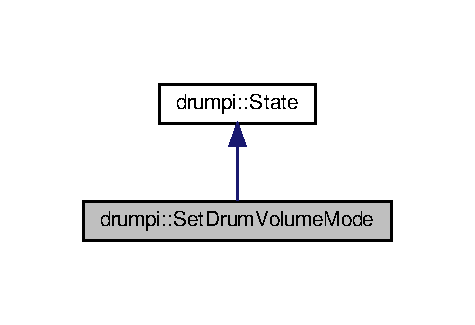
\includegraphics[width=244pt]{classdrumpi_1_1SetDrumVolumeMode__coll__graph}
\end{center}
\end{figure}
\doxysubsection*{Public Member Functions}
\begin{DoxyCompactItemize}
\item 
\mbox{\hyperlink{classdrumpi_1_1SetDrumVolumeMode_a14818c6a553e0f9ba0fedd51f2842019}{Set\+Drum\+Volume\+Mode}} ()
\item 
bool \mbox{\hyperlink{classdrumpi_1_1SetDrumVolumeMode_a6b0029ed8934700699658f3b85a67639}{interpret\+Key\+Press}} (\mbox{\hyperlink{classdrumpi_1_1ApplicationCallback}{Application\+Callback}} $\ast$appc, int key) override
\begin{DoxyCompactList}\small\item\em Performs an action depending on the key pressed. \end{DoxyCompactList}\item 
void \mbox{\hyperlink{classdrumpi_1_1SetDrumVolumeMode_aee11645a25952da9cf8cbddf995f7b96}{update\+Display}} (\mbox{\hyperlink{classdrumpi_1_1ApplicationCallback}{Application\+Callback}} $\ast$appc) override
\end{DoxyCompactItemize}
\doxysubsection*{Private Attributes}
\begin{DoxyCompactItemize}
\item 
\mbox{\hyperlink{namespacedrumpi_ad560bde7b693769d2c5882437af094bf}{drum\+I\+D\+\_\+t}} \mbox{\hyperlink{classdrumpi_1_1SetDrumVolumeMode_aff08b8d0e7225b9fcdbda60f214b7c2d}{drumselected}}
\item 
bool \mbox{\hyperlink{classdrumpi_1_1SetDrumVolumeMode_a3f4b7caa7b969ad360e1306a239254e4}{trigger\+Drums}}
\end{DoxyCompactItemize}
\doxysubsection*{Additional Inherited Members}


\doxysubsection{Detailed Description}
Set individual drum volumes in this state. 

\doxysubsection{Constructor \& Destructor Documentation}
\mbox{\Hypertarget{classdrumpi_1_1SetDrumVolumeMode_a14818c6a553e0f9ba0fedd51f2842019}\label{classdrumpi_1_1SetDrumVolumeMode_a14818c6a553e0f9ba0fedd51f2842019}} 
\index{drumpi::SetDrumVolumeMode@{drumpi::SetDrumVolumeMode}!SetDrumVolumeMode@{SetDrumVolumeMode}}
\index{SetDrumVolumeMode@{SetDrumVolumeMode}!drumpi::SetDrumVolumeMode@{drumpi::SetDrumVolumeMode}}
\doxysubsubsection{\texorpdfstring{SetDrumVolumeMode()}{SetDrumVolumeMode()}}
{\footnotesize\ttfamily Set\+Drum\+Volume\+Mode\+::\+Set\+Drum\+Volume\+Mode (\begin{DoxyParamCaption}{ }\end{DoxyParamCaption})}

Constructor 

\doxysubsection{Member Function Documentation}
\mbox{\Hypertarget{classdrumpi_1_1SetDrumVolumeMode_a6b0029ed8934700699658f3b85a67639}\label{classdrumpi_1_1SetDrumVolumeMode_a6b0029ed8934700699658f3b85a67639}} 
\index{drumpi::SetDrumVolumeMode@{drumpi::SetDrumVolumeMode}!interpretKeyPress@{interpretKeyPress}}
\index{interpretKeyPress@{interpretKeyPress}!drumpi::SetDrumVolumeMode@{drumpi::SetDrumVolumeMode}}
\doxysubsubsection{\texorpdfstring{interpretKeyPress()}{interpretKeyPress()}}
{\footnotesize\ttfamily bool Set\+Drum\+Volume\+Mode\+::interpret\+Key\+Press (\begin{DoxyParamCaption}\item[{\mbox{\hyperlink{classdrumpi_1_1ApplicationCallback}{Application\+Callback}} $\ast$}]{appc,  }\item[{int}]{key }\end{DoxyParamCaption})\hspace{0.3cm}{\ttfamily [override]}, {\ttfamily [virtual]}}



Performs an action depending on the key pressed. 

This method is called by the \mbox{\hyperlink{classdrumpi_1_1Application}{Application}} when a keyboard event occurs and the application is in \mbox{\hyperlink{classdrumpi_1_1SetDrumVolumeMode}{Set\+Drum\+Volume\+Mode}}. 
\begin{DoxyParams}{Parameters}
{\em appc} & Callback to the main \mbox{\hyperlink{classdrumpi_1_1Application}{Application}}. \\
\hline
{\em key} & The keypress detected. \\
\hline
\end{DoxyParams}


Implements \mbox{\hyperlink{classdrumpi_1_1State_aaa6205d85513b3f717c126e0717e1dbd}{drumpi\+::\+State}}.

\mbox{\Hypertarget{classdrumpi_1_1SetDrumVolumeMode_aee11645a25952da9cf8cbddf995f7b96}\label{classdrumpi_1_1SetDrumVolumeMode_aee11645a25952da9cf8cbddf995f7b96}} 
\index{drumpi::SetDrumVolumeMode@{drumpi::SetDrumVolumeMode}!updateDisplay@{updateDisplay}}
\index{updateDisplay@{updateDisplay}!drumpi::SetDrumVolumeMode@{drumpi::SetDrumVolumeMode}}
\doxysubsubsection{\texorpdfstring{updateDisplay()}{updateDisplay()}}
{\footnotesize\ttfamily void Set\+Drum\+Volume\+Mode\+::update\+Display (\begin{DoxyParamCaption}\item[{\mbox{\hyperlink{classdrumpi_1_1ApplicationCallback}{Application\+Callback}} $\ast$}]{appc }\end{DoxyParamCaption})\hspace{0.3cm}{\ttfamily [override]}, {\ttfamily [virtual]}}

Virtual function to be overridden by derived class. 

Implements \mbox{\hyperlink{classdrumpi_1_1State_a400c5fc605ddec1e4fe18c361bf38ef2}{drumpi\+::\+State}}.



\doxysubsection{Member Data Documentation}
\mbox{\Hypertarget{classdrumpi_1_1SetDrumVolumeMode_aff08b8d0e7225b9fcdbda60f214b7c2d}\label{classdrumpi_1_1SetDrumVolumeMode_aff08b8d0e7225b9fcdbda60f214b7c2d}} 
\index{drumpi::SetDrumVolumeMode@{drumpi::SetDrumVolumeMode}!drumselected@{drumselected}}
\index{drumselected@{drumselected}!drumpi::SetDrumVolumeMode@{drumpi::SetDrumVolumeMode}}
\doxysubsubsection{\texorpdfstring{drumselected}{drumselected}}
{\footnotesize\ttfamily \mbox{\hyperlink{namespacedrumpi_ad560bde7b693769d2c5882437af094bf}{drum\+I\+D\+\_\+t}} drumpi\+::\+Set\+Drum\+Volume\+Mode\+::drumselected\hspace{0.3cm}{\ttfamily [private]}}

Drum volume currently selected to be modified. \mbox{\Hypertarget{classdrumpi_1_1SetDrumVolumeMode_a3f4b7caa7b969ad360e1306a239254e4}\label{classdrumpi_1_1SetDrumVolumeMode_a3f4b7caa7b969ad360e1306a239254e4}} 
\index{drumpi::SetDrumVolumeMode@{drumpi::SetDrumVolumeMode}!triggerDrums@{triggerDrums}}
\index{triggerDrums@{triggerDrums}!drumpi::SetDrumVolumeMode@{drumpi::SetDrumVolumeMode}}
\doxysubsubsection{\texorpdfstring{triggerDrums}{triggerDrums}}
{\footnotesize\ttfamily bool drumpi\+::\+Set\+Drum\+Volume\+Mode\+::trigger\+Drums\hspace{0.3cm}{\ttfamily [private]}}

Whether to trigger the sounds on volume change. 

The documentation for this class was generated from the following files\+:\begin{DoxyCompactItemize}
\item 
src/application.\+hpp\item 
src/application.\+cpp\end{DoxyCompactItemize}

\hypertarget{classdrumpi_1_1SetMasterVolumeMode}{}\doxysection{drumpi\+::Set\+Master\+Volume\+Mode Class Reference}
\label{classdrumpi_1_1SetMasterVolumeMode}\index{drumpi::SetMasterVolumeMode@{drumpi::SetMasterVolumeMode}}


{\ttfamily \#include $<$application.\+hpp$>$}



Inheritance diagram for drumpi\+::Set\+Master\+Volume\+Mode\+:\nopagebreak
\begin{figure}[H]
\begin{center}
\leavevmode
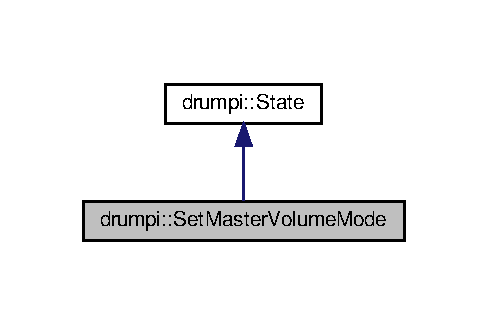
\includegraphics[width=250pt]{classdrumpi_1_1SetMasterVolumeMode__inherit__graph}
\end{center}
\end{figure}


Collaboration diagram for drumpi\+::Set\+Master\+Volume\+Mode\+:\nopagebreak
\begin{figure}[H]
\begin{center}
\leavevmode
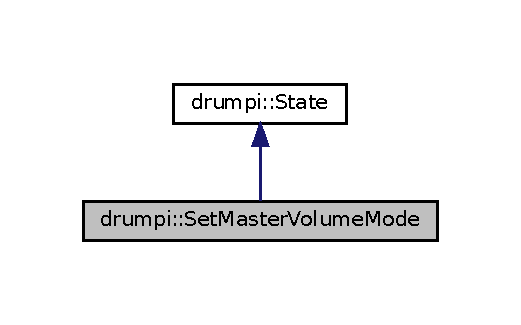
\includegraphics[width=250pt]{classdrumpi_1_1SetMasterVolumeMode__coll__graph}
\end{center}
\end{figure}
\doxysubsection*{Public Member Functions}
\begin{DoxyCompactItemize}
\item 
\mbox{\hyperlink{classdrumpi_1_1SetMasterVolumeMode_a0b8ba5fbd8da846136ffcde88364fc94}{Set\+Master\+Volume\+Mode}} ()
\item 
bool \mbox{\hyperlink{classdrumpi_1_1SetMasterVolumeMode_a18b5f4d0181ea1fbfd958afc473e240f}{interpret\+Key\+Press}} (\mbox{\hyperlink{classdrumpi_1_1ApplicationCallback}{Application\+Callback}} $\ast$appc, int key) override
\begin{DoxyCompactList}\small\item\em Performs an action depending on the key pressed. \end{DoxyCompactList}\item 
void \mbox{\hyperlink{classdrumpi_1_1SetMasterVolumeMode_ad8637f24eb5a7c11d829b8d41a9c46f2}{update\+Display}} (\mbox{\hyperlink{classdrumpi_1_1ApplicationCallback}{Application\+Callback}} $\ast$appc) override
\end{DoxyCompactItemize}
\doxysubsection*{Additional Inherited Members}


\doxysubsection{Detailed Description}
Set the master volume in this state (default). 

\doxysubsection{Constructor \& Destructor Documentation}
\mbox{\Hypertarget{classdrumpi_1_1SetMasterVolumeMode_a0b8ba5fbd8da846136ffcde88364fc94}\label{classdrumpi_1_1SetMasterVolumeMode_a0b8ba5fbd8da846136ffcde88364fc94}} 
\index{drumpi::SetMasterVolumeMode@{drumpi::SetMasterVolumeMode}!SetMasterVolumeMode@{SetMasterVolumeMode}}
\index{SetMasterVolumeMode@{SetMasterVolumeMode}!drumpi::SetMasterVolumeMode@{drumpi::SetMasterVolumeMode}}
\doxysubsubsection{\texorpdfstring{SetMasterVolumeMode()}{SetMasterVolumeMode()}}
{\footnotesize\ttfamily Set\+Master\+Volume\+Mode\+::\+Set\+Master\+Volume\+Mode (\begin{DoxyParamCaption}{ }\end{DoxyParamCaption})}

Constructor. 

\doxysubsection{Member Function Documentation}
\mbox{\Hypertarget{classdrumpi_1_1SetMasterVolumeMode_a18b5f4d0181ea1fbfd958afc473e240f}\label{classdrumpi_1_1SetMasterVolumeMode_a18b5f4d0181ea1fbfd958afc473e240f}} 
\index{drumpi::SetMasterVolumeMode@{drumpi::SetMasterVolumeMode}!interpretKeyPress@{interpretKeyPress}}
\index{interpretKeyPress@{interpretKeyPress}!drumpi::SetMasterVolumeMode@{drumpi::SetMasterVolumeMode}}
\doxysubsubsection{\texorpdfstring{interpretKeyPress()}{interpretKeyPress()}}
{\footnotesize\ttfamily bool Set\+Master\+Volume\+Mode\+::interpret\+Key\+Press (\begin{DoxyParamCaption}\item[{\mbox{\hyperlink{classdrumpi_1_1ApplicationCallback}{Application\+Callback}} $\ast$}]{appc,  }\item[{int}]{key }\end{DoxyParamCaption})\hspace{0.3cm}{\ttfamily [override]}, {\ttfamily [virtual]}}



Performs an action depending on the key pressed. 

This method is called by the \mbox{\hyperlink{classdrumpi_1_1Application}{Application}} when the applicaton is in either performance or sequencer mode and . or , are pressed. 
\begin{DoxyParams}{Parameters}
{\em appc} & Callback to the main \mbox{\hyperlink{classdrumpi_1_1Application}{Application}}. \\
\hline
{\em key} & The keypress detected. \\
\hline
\end{DoxyParams}


Implements \mbox{\hyperlink{classdrumpi_1_1State_aaa6205d85513b3f717c126e0717e1dbd}{drumpi\+::\+State}}.

\mbox{\Hypertarget{classdrumpi_1_1SetMasterVolumeMode_ad8637f24eb5a7c11d829b8d41a9c46f2}\label{classdrumpi_1_1SetMasterVolumeMode_ad8637f24eb5a7c11d829b8d41a9c46f2}} 
\index{drumpi::SetMasterVolumeMode@{drumpi::SetMasterVolumeMode}!updateDisplay@{updateDisplay}}
\index{updateDisplay@{updateDisplay}!drumpi::SetMasterVolumeMode@{drumpi::SetMasterVolumeMode}}
\doxysubsubsection{\texorpdfstring{updateDisplay()}{updateDisplay()}}
{\footnotesize\ttfamily void Set\+Master\+Volume\+Mode\+::update\+Display (\begin{DoxyParamCaption}\item[{\mbox{\hyperlink{classdrumpi_1_1ApplicationCallback}{Application\+Callback}} $\ast$}]{appc }\end{DoxyParamCaption})\hspace{0.3cm}{\ttfamily [override]}, {\ttfamily [virtual]}}

Virtual function to be overridden by derived class. 

Implements \mbox{\hyperlink{classdrumpi_1_1State_a400c5fc605ddec1e4fe18c361bf38ef2}{drumpi\+::\+State}}.



The documentation for this class was generated from the following files\+:\begin{DoxyCompactItemize}
\item 
src/application.\+hpp\item 
src/application.\+cpp\end{DoxyCompactItemize}

\hypertarget{classdrumpi_1_1SetTempoMode}{}\section{drumpi\+:\+:Set\+Tempo\+Mode Class Reference}
\label{classdrumpi_1_1SetTempoMode}\index{drumpi\+::\+Set\+Tempo\+Mode@{drumpi\+::\+Set\+Tempo\+Mode}}


{\ttfamily \#include $<$application.\+hpp$>$}



Inheritance diagram for drumpi\+:\+:Set\+Tempo\+Mode\+:
\nopagebreak
\begin{figure}[H]
\begin{center}
\leavevmode
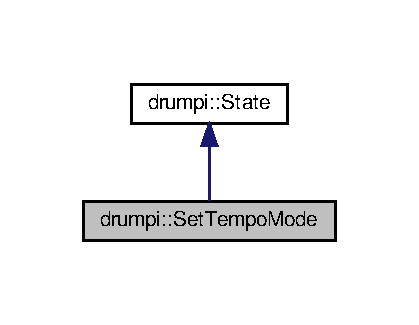
\includegraphics[width=201pt]{classdrumpi_1_1SetTempoMode__inherit__graph}
\end{center}
\end{figure}


Collaboration diagram for drumpi\+:\+:Set\+Tempo\+Mode\+:
\nopagebreak
\begin{figure}[H]
\begin{center}
\leavevmode
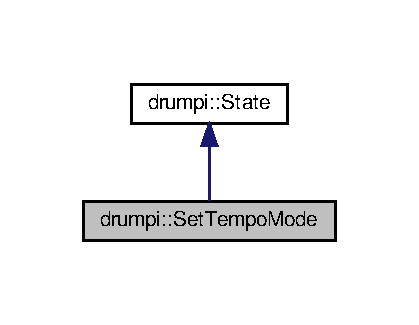
\includegraphics[width=201pt]{classdrumpi_1_1SetTempoMode__coll__graph}
\end{center}
\end{figure}
\subsection*{Public Member Functions}
\begin{DoxyCompactItemize}
\item 
\hyperlink{classdrumpi_1_1SetTempoMode_a2ddc51d8297abf394d91b3cb77d746d2}{Set\+Tempo\+Mode} ()
\item 
bool \hyperlink{classdrumpi_1_1SetTempoMode_a659f307caf23a57e3319ff6c510d41bf}{interpret\+Key\+Press} (\hyperlink{classdrumpi_1_1ApplicationCallback}{Application\+Callback} $\ast$appc, int key) override
\begin{DoxyCompactList}\small\item\em Performs an action depending on the key pressed. \end{DoxyCompactList}\item 
void \hyperlink{classdrumpi_1_1SetTempoMode_a965294425ec5abfccd8e3cbb9f1dbc3d}{update\+Display} (\hyperlink{classdrumpi_1_1ApplicationCallback}{Application\+Callback} $\ast$appc) override
\end{DoxyCompactItemize}
\subsection*{Private Attributes}
\begin{DoxyCompactItemize}
\item 
const int \hyperlink{classdrumpi_1_1SetTempoMode_acfb74b197bfd795f732b6d9684848af0}{bpm\+Step} = 8
\item 
const int \hyperlink{classdrumpi_1_1SetTempoMode_ad63e356af339b7673cc8af6f7c0adac0}{min\+B\+PM} = 38 + \hyperlink{classdrumpi_1_1SetTempoMode_acfb74b197bfd795f732b6d9684848af0}{bpm\+Step}
\end{DoxyCompactItemize}
\subsection*{Additional Inherited Members}


\subsection{Detailed Description}
Set tempo in this state. 

\subsection{Constructor \& Destructor Documentation}
\mbox{\Hypertarget{classdrumpi_1_1SetTempoMode_a2ddc51d8297abf394d91b3cb77d746d2}\label{classdrumpi_1_1SetTempoMode_a2ddc51d8297abf394d91b3cb77d746d2}} 
\index{drumpi\+::\+Set\+Tempo\+Mode@{drumpi\+::\+Set\+Tempo\+Mode}!Set\+Tempo\+Mode@{Set\+Tempo\+Mode}}
\index{Set\+Tempo\+Mode@{Set\+Tempo\+Mode}!drumpi\+::\+Set\+Tempo\+Mode@{drumpi\+::\+Set\+Tempo\+Mode}}
\subsubsection{\texorpdfstring{Set\+Tempo\+Mode()}{SetTempoMode()}}
{\footnotesize\ttfamily Set\+Tempo\+Mode\+::\+Set\+Tempo\+Mode (\begin{DoxyParamCaption}{ }\end{DoxyParamCaption})}

Constructor 

\subsection{Member Function Documentation}
\mbox{\Hypertarget{classdrumpi_1_1SetTempoMode_a659f307caf23a57e3319ff6c510d41bf}\label{classdrumpi_1_1SetTempoMode_a659f307caf23a57e3319ff6c510d41bf}} 
\index{drumpi\+::\+Set\+Tempo\+Mode@{drumpi\+::\+Set\+Tempo\+Mode}!interpret\+Key\+Press@{interpret\+Key\+Press}}
\index{interpret\+Key\+Press@{interpret\+Key\+Press}!drumpi\+::\+Set\+Tempo\+Mode@{drumpi\+::\+Set\+Tempo\+Mode}}
\subsubsection{\texorpdfstring{interpret\+Key\+Press()}{interpretKeyPress()}}
{\footnotesize\ttfamily bool Set\+Tempo\+Mode\+::interpret\+Key\+Press (\begin{DoxyParamCaption}\item[{\hyperlink{classdrumpi_1_1ApplicationCallback}{Application\+Callback} $\ast$}]{appc,  }\item[{int}]{key }\end{DoxyParamCaption})\hspace{0.3cm}{\ttfamily [override]}, {\ttfamily [virtual]}}



Performs an action depending on the key pressed. 

This method is called by the \hyperlink{classdrumpi_1_1Application}{Application} when a keyboard event occurs and the application is in \hyperlink{classdrumpi_1_1SetTempoMode}{Set\+Tempo\+Mode}. 
\begin{DoxyParams}{Parameters}
{\em appc} & Callback to the main \hyperlink{classdrumpi_1_1Application}{Application}. \\
\hline
{\em key} & The keypress detected. \\
\hline
\end{DoxyParams}


Implements \hyperlink{classdrumpi_1_1State_aaa6205d85513b3f717c126e0717e1dbd}{drumpi\+::\+State}.

\mbox{\Hypertarget{classdrumpi_1_1SetTempoMode_a965294425ec5abfccd8e3cbb9f1dbc3d}\label{classdrumpi_1_1SetTempoMode_a965294425ec5abfccd8e3cbb9f1dbc3d}} 
\index{drumpi\+::\+Set\+Tempo\+Mode@{drumpi\+::\+Set\+Tempo\+Mode}!update\+Display@{update\+Display}}
\index{update\+Display@{update\+Display}!drumpi\+::\+Set\+Tempo\+Mode@{drumpi\+::\+Set\+Tempo\+Mode}}
\subsubsection{\texorpdfstring{update\+Display()}{updateDisplay()}}
{\footnotesize\ttfamily void Set\+Tempo\+Mode\+::update\+Display (\begin{DoxyParamCaption}\item[{\hyperlink{classdrumpi_1_1ApplicationCallback}{Application\+Callback} $\ast$}]{appc }\end{DoxyParamCaption})\hspace{0.3cm}{\ttfamily [override]}, {\ttfamily [virtual]}}

Virtual function to be overridden by derived class. 

Implements \hyperlink{classdrumpi_1_1State_a400c5fc605ddec1e4fe18c361bf38ef2}{drumpi\+::\+State}.



\subsection{Member Data Documentation}
\mbox{\Hypertarget{classdrumpi_1_1SetTempoMode_acfb74b197bfd795f732b6d9684848af0}\label{classdrumpi_1_1SetTempoMode_acfb74b197bfd795f732b6d9684848af0}} 
\index{drumpi\+::\+Set\+Tempo\+Mode@{drumpi\+::\+Set\+Tempo\+Mode}!bpm\+Step@{bpm\+Step}}
\index{bpm\+Step@{bpm\+Step}!drumpi\+::\+Set\+Tempo\+Mode@{drumpi\+::\+Set\+Tempo\+Mode}}
\subsubsection{\texorpdfstring{bpm\+Step}{bpmStep}}
{\footnotesize\ttfamily const int drumpi\+::\+Set\+Tempo\+Mode\+::bpm\+Step = 8\hspace{0.3cm}{\ttfamily [private]}}

Step size of the tempo inc/decrements. \mbox{\Hypertarget{classdrumpi_1_1SetTempoMode_ad63e356af339b7673cc8af6f7c0adac0}\label{classdrumpi_1_1SetTempoMode_ad63e356af339b7673cc8af6f7c0adac0}} 
\index{drumpi\+::\+Set\+Tempo\+Mode@{drumpi\+::\+Set\+Tempo\+Mode}!min\+B\+PM@{min\+B\+PM}}
\index{min\+B\+PM@{min\+B\+PM}!drumpi\+::\+Set\+Tempo\+Mode@{drumpi\+::\+Set\+Tempo\+Mode}}
\subsubsection{\texorpdfstring{min\+B\+PM}{minBPM}}
{\footnotesize\ttfamily const int drumpi\+::\+Set\+Tempo\+Mode\+::min\+B\+PM = 38 + \hyperlink{classdrumpi_1_1SetTempoMode_acfb74b197bfd795f732b6d9684848af0}{bpm\+Step}\hspace{0.3cm}{\ttfamily [private]}}

Minimum B\+PM. 

The documentation for this class was generated from the following files\+:\begin{DoxyCompactItemize}
\item 
src/application.\+hpp\item 
src/application.\+cpp\end{DoxyCompactItemize}

\hypertarget{classdrumpi_1_1State}{}\section{drumpi\+:\+:State Class Reference}
\label{classdrumpi_1_1State}\index{drumpi\+::\+State@{drumpi\+::\+State}}


{\ttfamily \#include $<$application.\+hpp$>$}



Inheritance diagram for drumpi\+:\+:State\+:
\nopagebreak
\begin{figure}[H]
\begin{center}
\leavevmode
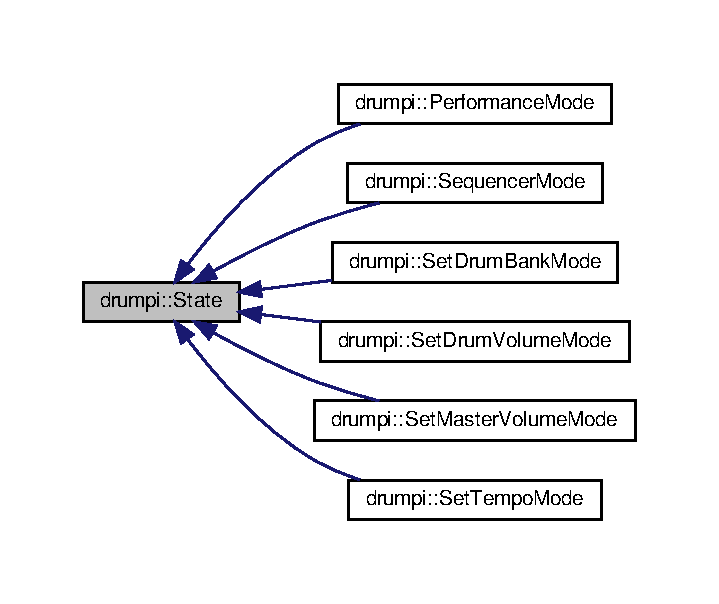
\includegraphics[width=345pt]{classdrumpi_1_1State__inherit__graph}
\end{center}
\end{figure}
\subsection*{Public Member Functions}
\begin{DoxyCompactItemize}
\item 
virtual bool \hyperlink{classdrumpi_1_1State_aaa6205d85513b3f717c126e0717e1dbd}{interpret\+Key\+Press} (\hyperlink{classdrumpi_1_1ApplicationCallback}{Application\+Callback} $\ast$appc, int key)=0
\item 
virtual void \hyperlink{classdrumpi_1_1State_a400c5fc605ddec1e4fe18c361bf38ef2}{update\+Display} (\hyperlink{classdrumpi_1_1ApplicationCallback}{Application\+Callback} $\ast$appc)=0
\item 
\hyperlink{namespacedrumpi_a3897274035c1b939a604438abe648b1b}{drum\+I\+D\+\_\+t} \hyperlink{classdrumpi_1_1State_a39b749a9049a4810935459c82aa42e6d}{interpret\+Drum\+Key} (int key)
\end{DoxyCompactItemize}
\subsection*{Public Attributes}
\begin{DoxyCompactItemize}
\item 
\hyperlink{namespacedrumpi_af70ab0854d65f24f7fa353fdc1c46bc9}{state\+Label\+\_\+t} \hyperlink{classdrumpi_1_1State_a6ddcdfba0e31dfb5182a7eaa6563f527}{label}
\end{DoxyCompactItemize}


\subsection{Detailed Description}
Abstract state class. 

\subsection{Member Function Documentation}
\mbox{\Hypertarget{classdrumpi_1_1State_a39b749a9049a4810935459c82aa42e6d}\label{classdrumpi_1_1State_a39b749a9049a4810935459c82aa42e6d}} 
\index{drumpi\+::\+State@{drumpi\+::\+State}!interpret\+Drum\+Key@{interpret\+Drum\+Key}}
\index{interpret\+Drum\+Key@{interpret\+Drum\+Key}!drumpi\+::\+State@{drumpi\+::\+State}}
\subsubsection{\texorpdfstring{interpret\+Drum\+Key()}{interpretDrumKey()}}
{\footnotesize\ttfamily \hyperlink{namespacedrumpi_a3897274035c1b939a604438abe648b1b}{drum\+I\+D\+\_\+t} State\+::interpret\+Drum\+Key (\begin{DoxyParamCaption}\item[{int}]{key }\end{DoxyParamCaption})}

Interprets drum keys and returns a drum ID. 
\begin{DoxyParams}{Parameters}
{\em key} & Keypress detected by \hyperlink{classdrumpi_1_1KeyboardInput}{Keyboard\+Input} class. \\
\hline
\end{DoxyParams}
\mbox{\Hypertarget{classdrumpi_1_1State_aaa6205d85513b3f717c126e0717e1dbd}\label{classdrumpi_1_1State_aaa6205d85513b3f717c126e0717e1dbd}} 
\index{drumpi\+::\+State@{drumpi\+::\+State}!interpret\+Key\+Press@{interpret\+Key\+Press}}
\index{interpret\+Key\+Press@{interpret\+Key\+Press}!drumpi\+::\+State@{drumpi\+::\+State}}
\subsubsection{\texorpdfstring{interpret\+Key\+Press()}{interpretKeyPress()}}
{\footnotesize\ttfamily virtual bool drumpi\+::\+State\+::interpret\+Key\+Press (\begin{DoxyParamCaption}\item[{\hyperlink{classdrumpi_1_1ApplicationCallback}{Application\+Callback} $\ast$}]{appc,  }\item[{int}]{key }\end{DoxyParamCaption})\hspace{0.3cm}{\ttfamily [pure virtual]}}

Virtual function to be overridden by derived class. 

Implemented in \hyperlink{classdrumpi_1_1SetDrumBankMode_a9b63a16aa08551a743c3751fa385c83b}{drumpi\+::\+Set\+Drum\+Bank\+Mode}, \hyperlink{classdrumpi_1_1SetDrumVolumeMode_a6b0029ed8934700699658f3b85a67639}{drumpi\+::\+Set\+Drum\+Volume\+Mode}, \hyperlink{classdrumpi_1_1SetMasterVolumeMode_a18b5f4d0181ea1fbfd958afc473e240f}{drumpi\+::\+Set\+Master\+Volume\+Mode}, \hyperlink{classdrumpi_1_1SetTempoMode_a659f307caf23a57e3319ff6c510d41bf}{drumpi\+::\+Set\+Tempo\+Mode}, \hyperlink{classdrumpi_1_1SequencerMode_aaa5dea1ffd66792ba62afae00820ffc6}{drumpi\+::\+Sequencer\+Mode}, and \hyperlink{classdrumpi_1_1PerformanceMode_a37c7c2eed9185a2211e389eebfd60262}{drumpi\+::\+Performance\+Mode}.

\mbox{\Hypertarget{classdrumpi_1_1State_a400c5fc605ddec1e4fe18c361bf38ef2}\label{classdrumpi_1_1State_a400c5fc605ddec1e4fe18c361bf38ef2}} 
\index{drumpi\+::\+State@{drumpi\+::\+State}!update\+Display@{update\+Display}}
\index{update\+Display@{update\+Display}!drumpi\+::\+State@{drumpi\+::\+State}}
\subsubsection{\texorpdfstring{update\+Display()}{updateDisplay()}}
{\footnotesize\ttfamily virtual void drumpi\+::\+State\+::update\+Display (\begin{DoxyParamCaption}\item[{\hyperlink{classdrumpi_1_1ApplicationCallback}{Application\+Callback} $\ast$}]{appc }\end{DoxyParamCaption})\hspace{0.3cm}{\ttfamily [pure virtual]}}

Virtual function to be overridden by derived class. 

Implemented in \hyperlink{classdrumpi_1_1SetDrumBankMode_ae2f14f230923c5e0c19c780c59328822}{drumpi\+::\+Set\+Drum\+Bank\+Mode}, \hyperlink{classdrumpi_1_1SetDrumVolumeMode_aee11645a25952da9cf8cbddf995f7b96}{drumpi\+::\+Set\+Drum\+Volume\+Mode}, \hyperlink{classdrumpi_1_1SetMasterVolumeMode_ad8637f24eb5a7c11d829b8d41a9c46f2}{drumpi\+::\+Set\+Master\+Volume\+Mode}, \hyperlink{classdrumpi_1_1SetTempoMode_a965294425ec5abfccd8e3cbb9f1dbc3d}{drumpi\+::\+Set\+Tempo\+Mode}, \hyperlink{classdrumpi_1_1SequencerMode_a0308bc9641daff4f48d74f9d2493d123}{drumpi\+::\+Sequencer\+Mode}, and \hyperlink{classdrumpi_1_1PerformanceMode_afc7bfd820bb21e4003ffe9ef189fa290}{drumpi\+::\+Performance\+Mode}.



\subsection{Member Data Documentation}
\mbox{\Hypertarget{classdrumpi_1_1State_a6ddcdfba0e31dfb5182a7eaa6563f527}\label{classdrumpi_1_1State_a6ddcdfba0e31dfb5182a7eaa6563f527}} 
\index{drumpi\+::\+State@{drumpi\+::\+State}!label@{label}}
\index{label@{label}!drumpi\+::\+State@{drumpi\+::\+State}}
\subsubsection{\texorpdfstring{label}{label}}
{\footnotesize\ttfamily \hyperlink{namespacedrumpi_af70ab0854d65f24f7fa353fdc1c46bc9}{state\+Label\+\_\+t} drumpi\+::\+State\+::label}

Label describing state type. 

The documentation for this class was generated from the following files\+:\begin{DoxyCompactItemize}
\item 
src/application.\+hpp\item 
src/application.\+cpp\end{DoxyCompactItemize}

\hypertarget{classdrumpi_1_1clock_1_1Timer}{}\doxysection{drumpi\+::clock\+::Timer Class Reference}
\label{classdrumpi_1_1clock_1_1Timer}\index{drumpi::clock::Timer@{drumpi::clock::Timer}}


{\ttfamily \#include $<$clock.\+hpp$>$}



Inheritance diagram for drumpi\+::clock\+::Timer\+:\nopagebreak
\begin{figure}[H]
\begin{center}
\leavevmode
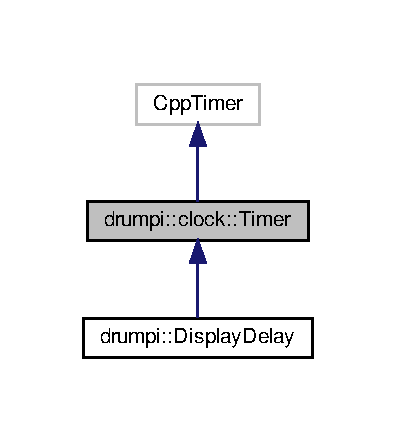
\includegraphics[width=202pt]{classdrumpi_1_1clock_1_1Timer__inherit__graph}
\end{center}
\end{figure}


Collaboration diagram for drumpi\+::clock\+::Timer\+:\nopagebreak
\begin{figure}[H]
\begin{center}
\leavevmode
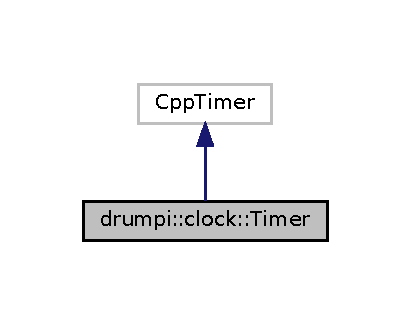
\includegraphics[width=197pt]{classdrumpi_1_1clock_1_1Timer__coll__graph}
\end{center}
\end{figure}
\doxysubsection*{Public Member Functions}
\begin{DoxyCompactItemize}
\item 
\mbox{\hyperlink{classdrumpi_1_1clock_1_1Timer_a5f16e8da27d2a5a5242dead46de05d97}{Timer}} ()
\item 
\mbox{\hyperlink{classdrumpi_1_1clock_1_1Timer_a14fa469c4c295c5fa6e66a4ad1092146}{$\sim$\+Timer}} ()
\item 
void \mbox{\hyperlink{classdrumpi_1_1clock_1_1Timer_a0a079d37a70001bfd23754d091db555d}{set\+Time}} (int ms)
\item 
int \mbox{\hyperlink{classdrumpi_1_1clock_1_1Timer_a5f9d0c70ff7666713743f5ee2180b9b4}{get\+Time}} ()
\item 
void \mbox{\hyperlink{classdrumpi_1_1clock_1_1Timer_a3a8b5272198d029779dc9302a54305a8}{start}} ()
\item 
void \mbox{\hyperlink{classdrumpi_1_1clock_1_1Timer_a63f0eb44b27402196590a03781515dba}{stop}} ()
\item 
bool \mbox{\hyperlink{classdrumpi_1_1clock_1_1Timer_ae675038252bdd55e0d42a92535025ee1}{is\+Active}} ()
\item 
virtual void \mbox{\hyperlink{classdrumpi_1_1clock_1_1Timer_aeed4c4e653b98280354e0b970f8df68b}{trigger}} ()=0
\end{DoxyCompactItemize}
\doxysubsection*{Private Member Functions}
\begin{DoxyCompactItemize}
\item 
void \mbox{\hyperlink{classdrumpi_1_1clock_1_1Timer_ab7328c35aba7b6887eea4bb6f90c5659}{timer\+Event}} () override
\end{DoxyCompactItemize}
\doxysubsection*{Private Attributes}
\begin{DoxyCompactItemize}
\item 
int \mbox{\hyperlink{classdrumpi_1_1clock_1_1Timer_a34ceb43c3f8fa2fd42f73aefb133497b}{time}}
\item 
bool \mbox{\hyperlink{classdrumpi_1_1clock_1_1Timer_a6a750b89a375a5f73f2d28ac951c0d24}{active}}
\end{DoxyCompactItemize}


\doxysubsection{Detailed Description}
Trigger a single delayed action. To use, create a class that inherits from this and override the \mbox{\hyperlink{classdrumpi_1_1clock_1_1Timer_aeed4c4e653b98280354e0b970f8df68b}{trigger}} method to set the functionality. 

\doxysubsection{Constructor \& Destructor Documentation}
\mbox{\Hypertarget{classdrumpi_1_1clock_1_1Timer_a5f16e8da27d2a5a5242dead46de05d97}\label{classdrumpi_1_1clock_1_1Timer_a5f16e8da27d2a5a5242dead46de05d97}} 
\index{drumpi::clock::Timer@{drumpi::clock::Timer}!Timer@{Timer}}
\index{Timer@{Timer}!drumpi::clock::Timer@{drumpi::clock::Timer}}
\doxysubsubsection{\texorpdfstring{Timer()}{Timer()}}
{\footnotesize\ttfamily Timer\+::\+Timer (\begin{DoxyParamCaption}{ }\end{DoxyParamCaption})}

Constructor. \mbox{\Hypertarget{classdrumpi_1_1clock_1_1Timer_a14fa469c4c295c5fa6e66a4ad1092146}\label{classdrumpi_1_1clock_1_1Timer_a14fa469c4c295c5fa6e66a4ad1092146}} 
\index{drumpi::clock::Timer@{drumpi::clock::Timer}!````~Timer@{$\sim$Timer}}
\index{````~Timer@{$\sim$Timer}!drumpi::clock::Timer@{drumpi::clock::Timer}}
\doxysubsubsection{\texorpdfstring{$\sim$Timer()}{~Timer()}}
{\footnotesize\ttfamily Timer\+::$\sim$\+Timer (\begin{DoxyParamCaption}{ }\end{DoxyParamCaption})}

Destructor. Deactivates the \mbox{\hyperlink{classdrumpi_1_1clock_1_1Timer}{Timer}}. 

\doxysubsection{Member Function Documentation}
\mbox{\Hypertarget{classdrumpi_1_1clock_1_1Timer_a5f9d0c70ff7666713743f5ee2180b9b4}\label{classdrumpi_1_1clock_1_1Timer_a5f9d0c70ff7666713743f5ee2180b9b4}} 
\index{drumpi::clock::Timer@{drumpi::clock::Timer}!getTime@{getTime}}
\index{getTime@{getTime}!drumpi::clock::Timer@{drumpi::clock::Timer}}
\doxysubsubsection{\texorpdfstring{getTime()}{getTime()}}
{\footnotesize\ttfamily int Timer\+::get\+Time (\begin{DoxyParamCaption}{ }\end{DoxyParamCaption})}

Returns the trigger time in ms. \begin{DoxyReturn}{Returns}
trigger time in ms. 
\end{DoxyReturn}
\mbox{\Hypertarget{classdrumpi_1_1clock_1_1Timer_ae675038252bdd55e0d42a92535025ee1}\label{classdrumpi_1_1clock_1_1Timer_ae675038252bdd55e0d42a92535025ee1}} 
\index{drumpi::clock::Timer@{drumpi::clock::Timer}!isActive@{isActive}}
\index{isActive@{isActive}!drumpi::clock::Timer@{drumpi::clock::Timer}}
\doxysubsubsection{\texorpdfstring{isActive()}{isActive()}}
{\footnotesize\ttfamily bool Timer\+::is\+Active (\begin{DoxyParamCaption}{ }\end{DoxyParamCaption})}

Checks if the \mbox{\hyperlink{classdrumpi_1_1clock_1_1Timer}{Timer}} is active. \begin{DoxyReturn}{Returns}
{\ttfamily true} if active. 
\end{DoxyReturn}
\mbox{\Hypertarget{classdrumpi_1_1clock_1_1Timer_a0a079d37a70001bfd23754d091db555d}\label{classdrumpi_1_1clock_1_1Timer_a0a079d37a70001bfd23754d091db555d}} 
\index{drumpi::clock::Timer@{drumpi::clock::Timer}!setTime@{setTime}}
\index{setTime@{setTime}!drumpi::clock::Timer@{drumpi::clock::Timer}}
\doxysubsubsection{\texorpdfstring{setTime()}{setTime()}}
{\footnotesize\ttfamily void Timer\+::set\+Time (\begin{DoxyParamCaption}\item[{int}]{ms }\end{DoxyParamCaption})}

Set trigger time in ms. 
\begin{DoxyParams}{Parameters}
{\em ms} & desired trigger time in ms. \\
\hline
\end{DoxyParams}
\mbox{\Hypertarget{classdrumpi_1_1clock_1_1Timer_a3a8b5272198d029779dc9302a54305a8}\label{classdrumpi_1_1clock_1_1Timer_a3a8b5272198d029779dc9302a54305a8}} 
\index{drumpi::clock::Timer@{drumpi::clock::Timer}!start@{start}}
\index{start@{start}!drumpi::clock::Timer@{drumpi::clock::Timer}}
\doxysubsubsection{\texorpdfstring{start()}{start()}}
{\footnotesize\ttfamily void Timer\+::start (\begin{DoxyParamCaption}{ }\end{DoxyParamCaption})}

Start the \mbox{\hyperlink{classdrumpi_1_1clock_1_1Timer}{Timer}}. \mbox{\Hypertarget{classdrumpi_1_1clock_1_1Timer_a63f0eb44b27402196590a03781515dba}\label{classdrumpi_1_1clock_1_1Timer_a63f0eb44b27402196590a03781515dba}} 
\index{drumpi::clock::Timer@{drumpi::clock::Timer}!stop@{stop}}
\index{stop@{stop}!drumpi::clock::Timer@{drumpi::clock::Timer}}
\doxysubsubsection{\texorpdfstring{stop()}{stop()}}
{\footnotesize\ttfamily void Timer\+::stop (\begin{DoxyParamCaption}{ }\end{DoxyParamCaption})}

Cancels the \mbox{\hyperlink{classdrumpi_1_1clock_1_1Timer}{Timer}}. \mbox{\Hypertarget{classdrumpi_1_1clock_1_1Timer_ab7328c35aba7b6887eea4bb6f90c5659}\label{classdrumpi_1_1clock_1_1Timer_ab7328c35aba7b6887eea4bb6f90c5659}} 
\index{drumpi::clock::Timer@{drumpi::clock::Timer}!timerEvent@{timerEvent}}
\index{timerEvent@{timerEvent}!drumpi::clock::Timer@{drumpi::clock::Timer}}
\doxysubsubsection{\texorpdfstring{timerEvent()}{timerEvent()}}
{\footnotesize\ttfamily void Timer\+::timer\+Event (\begin{DoxyParamCaption}{ }\end{DoxyParamCaption})\hspace{0.3cm}{\ttfamily [override]}, {\ttfamily [private]}}

Override event method to call \mbox{\hyperlink{classdrumpi_1_1clock_1_1Timer_aeed4c4e653b98280354e0b970f8df68b}{trigger()}}. \mbox{\Hypertarget{classdrumpi_1_1clock_1_1Timer_aeed4c4e653b98280354e0b970f8df68b}\label{classdrumpi_1_1clock_1_1Timer_aeed4c4e653b98280354e0b970f8df68b}} 
\index{drumpi::clock::Timer@{drumpi::clock::Timer}!trigger@{trigger}}
\index{trigger@{trigger}!drumpi::clock::Timer@{drumpi::clock::Timer}}
\doxysubsubsection{\texorpdfstring{trigger()}{trigger()}}
{\footnotesize\ttfamily virtual void drumpi\+::clock\+::\+Timer\+::trigger (\begin{DoxyParamCaption}{ }\end{DoxyParamCaption})\hspace{0.3cm}{\ttfamily [pure virtual]}}

Callback method run when the time has passed. Override to add functionality. 

Implemented in \mbox{\hyperlink{classdrumpi_1_1DisplayDelay_a1fb66a57fea2d6700a190c961e556aa4}{drumpi\+::\+Display\+Delay}}.



\doxysubsection{Member Data Documentation}
\mbox{\Hypertarget{classdrumpi_1_1clock_1_1Timer_a6a750b89a375a5f73f2d28ac951c0d24}\label{classdrumpi_1_1clock_1_1Timer_a6a750b89a375a5f73f2d28ac951c0d24}} 
\index{drumpi::clock::Timer@{drumpi::clock::Timer}!active@{active}}
\index{active@{active}!drumpi::clock::Timer@{drumpi::clock::Timer}}
\doxysubsubsection{\texorpdfstring{active}{active}}
{\footnotesize\ttfamily bool drumpi\+::clock\+::\+Timer\+::active\hspace{0.3cm}{\ttfamily [private]}}

Active flag. \mbox{\Hypertarget{classdrumpi_1_1clock_1_1Timer_a34ceb43c3f8fa2fd42f73aefb133497b}\label{classdrumpi_1_1clock_1_1Timer_a34ceb43c3f8fa2fd42f73aefb133497b}} 
\index{drumpi::clock::Timer@{drumpi::clock::Timer}!time@{time}}
\index{time@{time}!drumpi::clock::Timer@{drumpi::clock::Timer}}
\doxysubsubsection{\texorpdfstring{time}{time}}
{\footnotesize\ttfamily int drumpi\+::clock\+::\+Timer\+::time\hspace{0.3cm}{\ttfamily [private]}}

Trigger time in ms. 

The documentation for this class was generated from the following files\+:\begin{DoxyCompactItemize}
\item 
src/clock.\+hpp\item 
src/clock.\+cpp\end{DoxyCompactItemize}

%--- End generated contents ---

% Index
\backmatter
\newpage
\phantomsection
\clearemptydoublepage
\addcontentsline{toc}{chapter}{Index}
\printindex

\end{document}
